%% Run LaTeX on this file several times to get Table of Contents,
%% cross-references, and citations.

\documentclass[11pt]{book}
\usepackage{gvv-book}
\usepackage{gvv}
%\usepackage{Wiley-AuthoringTemplate}
\usepackage[sectionbib,authoryear]{natbib}% for name-date citation comment the below line
%\usepackage[sectionbib,numbers]{natbib}% for numbered citation comment the above line

%%********************************************************************%%
%%       How many levels of section head would you like numbered?     %%
%% 0= no section numbers, 1= section, 2= subsection, 3= subsubsection %%
\setcounter{secnumdepth}{3}
%%********************************************************************%%
%%**********************************************************************%%
%%     How many levels of section head would you like to appear in the  %%
%%				Table of Contents?			%%
%% 0= chapter, 1= section, 2= subsection, 3= subsubsection titles.	%%
\setcounter{tocdepth}{2}
%%**********************************************************************%%

%\includeonly{ch01}
\makeindex

\begin{document}

\frontmatter
%%%%%%%%%%%%%%%%%%%%%%%%%%%%%%%%%%%%%%%%%%%%%%%%%%%%%%%%%%%%%%%%
%% Title Pages
%% Wiley will provide title and copyright page, but you can make
%% your own titlepages if you'd like anyway
%% Setting up title pages, type in the appropriate names here:

\booktitle{Digital Communication}

\subtitle{Through Simulations}

\AuAff{G. V. V. Sharma}


%% \\ will start a new line.
%% You may add \affil{} for affiliation, ie,
%\authors{Robert M. Groves\\
%\affil{Universitat de les Illes Balears}
%Floyd J. Fowler, Jr.\\
%\affil{University of New Mexico}
%}

%% Print Half Title and Title Page:
%\halftitlepage
\titlepage

%%%%%%%%%%%%%%%%%%%%%%%%%%%%%%%%%%%%%%%%%%%%%%%%%%%%%%%%%%%%%%%%
%% Copyright Page

\begin{copyrightpage}{2022}
%Title, etc
\end{copyrightpage}

% Note, you must use \ to start indented lines, ie,
% 
% \begin{copyrightpage}{2004}
% Survey Methodology / Robert M. Groves . . . [et al.].
% \       p. cm.---(Wiley series in survey methodology)
% \    ``Wiley-Interscience."
% \    Includes bibliographical references and index.
% \    ISBN 0-471-48348-6 (pbk.)
% \    1. Surveys---Methodology.  2. Social 
% \  sciences---Research---Statistical methods.  I. Groves, Robert M.  II. %
% Series.\\

% HA31.2.S873 2004
% 001.4'33---dc22                                             2004044064
% \end{copyrightpage}

%%%%%%%%%%%%%%%%%%%%%%%%%%%%%%%%%%%%%%%%%%%%%%%%%%%%%%%%%%%%%%%%
%% Only Dedication (optional) 

%\dedication{To my parents}

\tableofcontents

%\listoffigures %optional
%\listoftables  %optional

%% or Contributor Page for edited books
%% before \tableofcontents

%%%%%%%%%%%%%%%%%%%%%%%%%%%%%%%%%%%%%%%%%%%%%%%%%%%%%%%%%%%%%%%%
%  Contributors Page for Edited Book
%%%%%%%%%%%%%%%%%%%%%%%%%%%%%%%%%%%%%%%%%%%%%%%%%%%%%%%%%%%%%%%%

% If your book has chapters written by different authors,
% you'll need a Contributors page.

% Use \begin{contributors}...\end{contributors} and
% then enter each author with the \name{} command, followed
% by the affiliation information.

% \begin{contributors}
% \name{Masayki Abe,} Fujitsu Laboratories Ltd., Fujitsu Limited, Atsugi, Japan
%
% \name{L. A. Akers,} Center for Solid State Electronics Research, Arizona State University, Tempe, Arizona
%
% \name{G. H. Bernstein,} Department of Electrical and Computer Engineering, University of Notre Dame, Notre Dame, South Bend, Indiana; formerly of
% Center for Solid State Electronics Research, Arizona
% State University, Tempe, Arizona 
% \end{contributors}

%%%%%%%%%%%%%%%%%%%%%%%%%%%%%%%%%%%%%%%%%%%%%%%%%%%%%%%%%%%%%%%%
% Optional Foreword:

%\begin{foreword}
%\lipsum[1-2]
%\end{foreword}

%%%%%%%%%%%%%%%%%%%%%%%%%%%%%%%%%%%%%%%%%%%%%%%%%%%%%%%%%%%%%%%%
% Optional Preface:

%\begin{preface}
%\lipsum[1-1]
%\prefaceauthor{}
%\where{place\\
% date}
%\end{preface}

% ie,
% \begin{preface}
% This is an example preface.
% \prefaceauthor{R. K. Watts}
% \where{Durham, North Carolina\\
% September, 2004}

%%%%%%%%%%%%%%%%%%%%%%%%%%%%%%%%%%%%%%%%%%%%%%%%%%%%%%%%%%%%%%%%
% Optional Acknowledgments:

%\acknowledgments
%\lipsum[1-2]
%\authorinitials{I. R. S.}  

%%%%%%%%%%%%%%%%%%%%%%%%%%%%%%%%
%% Glossary Type of Environment:

% \begin{glossary}
% \term{<term>}{<description>}
% \end{glossary}

%%%%%%%%%%%%%%%%%%%%%%%%%%%%%%%%
%\begin{acronyms}
%\acro{ASTA}{Arrivals See Time Averages}
%\acro{BHCA}{Busy Hour Call Attempts}
%\acro{BR}{Bandwidth Reservation}
%\acro{b.u.}{bandwidth unit(s)}
%\acro{CAC}{Call / Connection Admission Control}
%\acro{CBP}{Call Blocking Probability(-ies)}
%\acro{CCS}{Centum Call Seconds}
%\acro{CDTM}{Connection Dependent Threshold Model}
%\acro{CS}{Complete Sharing}
%\acro{DiffServ}{Differentiated Services}
%\acro{EMLM}{Erlang Multirate Loss Model}
%\acro{erl}{The Erlang unit of traffic-load}
%\acro{FIFO}{First in - First out}
%\acro{GB}{Global balance}
%\acro{GoS}{Grade of Service}
%\acro{ICT}{Information and Communication Technology}
%\acro{IntServ}{Integrated Services}
%\acro{IP}{Internet Protocol}
%\acro{ITU-T}{International Telecommunication Unit -- Standardization sector}
%\acro{LB}{Local balance}
%\acro{LHS}{Left hand side}
%\acro{LIFO}{Last in - First out}
%\acro{MMPP}{Markov Modulated Poisson Process}
%\acro{MPLS}{Multiple Protocol Labeling Switching}
%\acro{MRM}{Multi-Retry Model}
%\acro{MTM}{Multi-Threshold Model}
%\acro{PASTA}{Poisson Arrivals See Time Averages}
%\acro{PDF}{Probability Distribution Function}
%\acro{pdf}{probability density function}
%\acro{PFS}{Product Form Solution}
%\acro{QoS}{Quality of Service}
%\acro{r.v.}{random variable(s)}
%\acro{RED}{random early detection}
%\acro{RHS}{Right hand side}
%\acro{RLA}{Reduced Load Approximation}
%\acro{SIRO}{service in random order}
%\acro{SRM}{Single-Retry Model}
%\acro{STM}{Single-Threshold Model}
%\acro{TCP}{Transport Control Protocol}
%\acro{TH}{Threshold(s)}
%\acro{UDP}{User Datagram Protocol}
%\end{acronyms}

\setcounter{page}{1}

\begin{introduction}
This book introduces digital communication through probability.

\end{introduction}

\mainmatter

\chapter{Introduction}
%\input{ncert/intro.tex}
\chapter{Axioms}
\section{Examples}
\begin{enumerate}[label=\thesection.\arabic*,ref=\thesection.\theenumi]
\item Given that the events A and B are such that $P(A)=\frac{1}{2}, P(A + B)=\frac{3}{5}$ and $P(B)=p$. Find $p$ if they are 
\begin{enumerate}
\item mutually exclusive
\item independent
\end{enumerate}
\iffalse
\documentclass[journal,12pt,twocolumn]{IEEEtran}
\usepackage{graphicx}
\graphicspath{{./figs/}}{}
\usepackage{amsmath,amssymb,amsfonts,amsthm}
\newcommand{\myvec}[1]{\ensuremath{\begin{pmatrix}#1\end{pmatrix}}}
\usepackage{listings}
\usepackage{watermark}
\usepackage{titlesec}
\let\vec\mathbf

\titlespacing{\subsection}{0pt}{\parskip}{-3pt}
\titlespacing{\subsubsection}{0pt}{\parskip}{-\parskip}
\titlespacing{\paragraph}{0pt}{\parskip}{\parskip}
\newcommand{\figuremacro}[5]{
    
}
\lstset{
frame=single, 
breaklines=true,
columns=fullflexible
}
\thiswatermark{\centering \put(0,-105.0}{\includegraphics[scale=0.5]{iith.png}} }

\sloppy
\title{\mytitle}
\title{
Probability Assignment-II
}
\author{Nikhil Nair}
\begin{document}
\maketitle
%\tableofcontents
\bigskip



\section{\textbf{Problem }}
\fi
\solution
\begin{enumerate}
	\item 
		In this case
\begin{align}
\pr{A + B} &=\pr{A} + \pr{B}&
\\
\implies \frac{3}{5}&=\frac{1}{2}+p&
\\
\therefore  p &= \frac{1}{10}&
\end{align}
\item 
Given A and B are independent events,
then,

\begin{align}
\pr{A + B} &=\pr{A} + \pr{B} - \pr{A B}& 
\\
\implies \pr{A + B} &=\pr{A} + \pr{B} - \pr{A}\pr{B}&
\\
\implies \frac{3}{5}&=\frac{1}{2}+ p - \frac{p}{2}&
\\
\therefore p &= \frac{1}{5}&
\end{align}
\end{enumerate}

\end{enumerate}

\section{Exercises}
\begin{enumerate}[label=\thesection.\arabic*,ref=\thesection.\theenumi]
	\item The accompanying Venn diagram in 
\figref{fig:exemplar/11/16/3/11/Venn_Diagram}
		shows three events, A, B, and C, and also the probabilities of the various intersections (for instance, \pr{AB} = .07). Determine
\begin{enumerate}
\item 
\pr{A}
\item 
\pr{BC^\prime}
\item 
\pr{A + B}
\item 
\pr{AB^\prime}
\item 
\pr{BC}
\item 
Probability of exactly one
of the three occurs.
\end{enumerate}
\begin{figure}[h!]
	\centering
	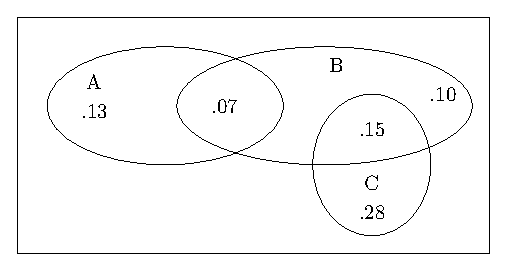
\includegraphics[width = \columnwidth]{exemplar/11/16/3/11/figs/new-figure0}
\caption{Question Figure}
\label{fig:exemplar/11/16/3/11/Venn_Diagram}
\end{figure}
		\solution
		\iffalse
\documentclass[journal,11pt,onecolumn]{IEEEtran}
\usepackage{setspace}
\usepackage{gensymb}
\singlespacing
\usepackage[cmex10]{amsmath}
\usepackage{amsthm}
\usepackage{mathrsfs}
\usepackage{txfonts}
\usepackage{stfloats}
\usepackage{bm}
\usepackage{cite}
\usepackage{cases}
\usepackage{subfig}
\usepackage{longtable}
\usepackage{multirow}
\usepackage{enumitem}
\usepackage{mathtools}
\usepackage{tikz}
\usepackage{circuitikz}
\usepackage{verbatim}
\usepackage[breaklinks=true]{hyperref}
\usepackage{tkz-euclide} % loads  TikZ and tkz-base
\usepackage{listings}
\usepackage{color}    
\usepackage{array}    
\usepackage{longtable}
\usepackage{calc}     
\usepackage{multirow} 
\usepackage{hhline}   
\usepackage{ifthen}   
\usepackage{lscape}     
\usepackage{chngcntr}
\usepackage{float}
\DeclareMathOperator*{\Res}{Res}
\renewcommand\thesection{\arabic{section}}
\renewcommand\thesubsection{\thesection.\arabic{subsection}}
\renewcommand\thesubsubsection{\thesubsection.\arabic{subsubsection}}

\renewcommand\thesectiondis{\arabic{section}}
\renewcommand\thesubsectiondis{\thesectiondis.\arabic{subsection}}
\renewcommand\thesubsubsectiondis{\thesubsectiondis.\arabic{subsubsection}}
\renewcommand\thetable{\arabic{table}}
% correct bad hyphenation here
\hyphenation{op-tical net-works semi-conduc-tor}
\def\inputGnumericTable{}                                 %%

\lstset{
%language=C,
frame=single, 
breaklines=true,
columns=fullflexible
}
%\lstset{
%language=tex,
%frame=single, 
%breaklines=true
%}

\title{Assignment}
\author{Barath surya M | EE22BTECH11014}
\begin{document}
\newtheorem{theorem}{Theorem}[section]
\newtheorem{problem}{Problem}
\newtheorem{proposition}{Proposition}[section]
\newtheorem{lemma}{Lemma}[section]
\newtheorem{corollary}[theorem]{Corollary}
\newtheorem{example}{Example}[section]
\newtheorem{definition}[problem]{Definition}
\newcommand{\BEQA}{\begin{eqnarray}}
\newcommand{\EEQA}{\end{eqnarray}}
\newcommand{\define}{\stackrel{\triangle}{=}}
\bibliographystyle{IEEEtran}
\providecommand{\mbf}{\mathbf}
\providecommand{\pr}[1]{\ensuremath{\Pr\left(#1\right)}}
\providecommand{\qfunc}[1]{\ensuremath{Q\left(#1\right)}}
\providecommand{\sbrak}[1]{\ensuremath{{}\left[#1\right]}}
\providecommand{\lsbrak}[1]{\ensuremath{{}\left[#1\right.}}
\providecommand{\rsbrak}[1]{\ensuremath{{}\left.#1\right]}}
\providecommand{\brak}[1]{\ensuremath{\left(#1\right)}}
\providecommand{\lbrak}[1]{\ensuremath{\left(#1\right.}}
\providecommand{\rbrak}[1]{\ensuremath{\left.#1\right)}}
\providecommand{\cbrak}[1]{\ensuremath{\left\{#1\right\}}}
\providecommand{\lcbrak}[1]{\ensuremath{\left\{#1\right.}}
\providecommand{\rcbrak}[1]{\ensuremath{\left.#1\right\}}}
\theoremstyle{remark}
\newtheorem{rem}{Remark}
\newcommand{\sgn}{\mathop{\mathrm{sgn}}}
\providecommand{\abs}[1]{\left\vert#1\right\vert}
\providecommand{\res}[1]{\Res\displaylimits_{#1}} 
\providecommand{\norm}[1]{\left\lVert#1\right\rVert}
\providecommand{\mtx}[1]{\mathbf{#1}}
\providecommand{\mean}[1]{E\left[ #1 \right]}
\providecommand{\fourier}{\overset{\mathcal{F}}{ \rightleftharpoons}}
\providecommand{\system}[1]{\overset{\mathcal{#1}}{ \longleftrightarrow}}
\newcommand{\solution}{\noindent \textbf{Solution: }}
\newcommand{\cosec}{\,\text{cosec}\,}
\providecommand{\dec}[2]{\ensuremath{\overset{#1}{\underset{#2}{\gtrless}}}}
\newcommand{\myvec}[1]{\ensuremath{\begin{pmatrix}#1\end{pmatrix}}}
\newcommand{\mydet}[1]{\ensuremath{\begin{vmatrix}#1\end{vmatrix}}}
\let\vec\mathbf
\def\putbox#1#2#3{\makebox[0in][l]{\makebox[#1][l]{}\raisebox{\baselineskip}[0in][0in]{\raisebox{#2}[0in][0in]{#3}}}}
     \def\rightbox#1{\makebox[0in][r]{#1}}
     \def\centbox#1{\makebox[0in]{#1}}
     \def\topbox#1{\raisebox{-\baselineskip}[0in][0in]{#1}}
     \def\midbox#1{\raisebox{-0.5\baselineskip}[0in][0in]{#1}}
\maketitle
\vspace{3cm}
Question 11.16.3.11\\
The accompanying venn diagram shows three events, A, B and C, and also the probabilities of the various intersections (for instance, $\pr{AB}=0.7$. Determine 
\begin{enumerate}
	\item \pr{A}
	\item \pr{BC'}
	\item \pr{A+B}
	\item \pr{AB'}
	\item \pr{BC}
	\item \text{Probability of exactly one of the three occurs}
\end{enumerate}
\begin{figure}[h!]
	\centering
	\tikzset{every picture/.style={line width=0.75pt}}   
 
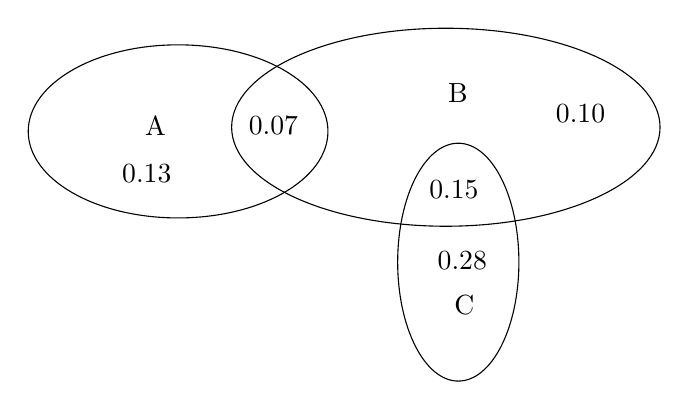
\begin{tikzpicture}[x=0.75pt,y=0.75pt,yscale=-1,xscale=1] 
 
\draw   (106,103.3) .. controls (106,80.27) and (138.33,61.6) .. (178.2,61.6) .. controls (218.07,61.6) and (250.4,80.27) .. (250.4,103.3) .. controls (250.4,126.33) and (218.07,145) .. (178.2,145) .. controls (138.33,145) and (106,126.33) .. (106,103.3) -- cycle ; 
\draw   (204,101.3) .. controls (204,74.96) and (250.2,53.6) .. (307.2,53.6) .. controls (364.2,53.6) and (410.4,74.96) .. (410.4,101.3) .. controls (410.4,127.64) and (364.2,149) .. (307.2,149) .. controls (250.2,149) and (204,127.64) .. (204,101.3) -- cycle ; 
\draw   (313.2,109) .. controls (329.33,109) and (342.4,134.65) .. (342.4,166.3) .. controls (342.4,197.95) and (329.33,223.6) .. (313.2,223.6) .. controls (297.07,223.6) and (284,197.95) .. (284,166.3) .. controls (284,134.65) and (297.07,109) .. (313.2,109) -- cycle ; 
 
\draw (161,95) node [anchor=north west][inner sep=0.75pt]   [align=left] {A}; 
\draw (307,79) node [anchor=north west][inner sep=0.75pt]   [align=left] {B}; 
\draw (310,181) node [anchor=north west][inner sep=0.75pt]   [align=left] {C}; 
\draw (150,118) node [anchor=north west][inner sep=0.75pt]   [align=left] {0.13}; 
\draw (211,95) node [anchor=north west][inner sep=0.75pt]   [align=left] {0.07}; 
\draw (298,126) node [anchor=north west][inner sep=0.75pt]   [align=left] {0.15}; 
\draw (359,89) node [anchor=north west][inner sep=0.75pt]   [align=left] {0.10}; 
\draw (302,160) node [anchor=north west][inner sep=0.75pt]   [align=left] {0.28\\}; 
 
 
\end{tikzpicture}

	\caption {generated by Latextikz}
	\label{fig:exemplar/11/16/3/11}
\end{figure}
\solution
\fi
Given:\\
From \figref{fig:exemplar/11/16/3/11}
\begin{align}
\pr{AB}=0.07\\
\pr{AB'}=0.13\\
\pr{BC}=0.15\\
\pr{BA'C'}=0.10\\
\pr{CB'}=0.28
\end{align}
\begin{enumerate}
\item \begin{align}
	\pr{A}&= 0.13+0.07\\
	&=0.2
	\end{align}
\item \begin{align}
	\pr{BC'} &=0.07+0.10+0.15-0.15\\
	&=0.17
\end{align}
\item \begin{align}
	\pr{A+B}&= \pr{A}+\pr{B} -\pr{AB}\\
	&=0.20+\brak{0.07+0.10+0.15}-0.07\\
	&=0.45
\end{align} 
\item \begin{align}
	\pr{AB'}&=0.20-0.07\\
	&=0.13
\end{align}
\item \begin{align}
	\pr{BC}&=0.15
\end{align} 
\item \begin{align}
	\pr{\text{AB'}} +\pr{CB'}+\pr{BA'C'} &= 0.13+0.10+0.28\\
	&=0.51
\end{align} 
\end{enumerate}


 

\end{enumerate}

\chapter{Random Variables}
\section{Examples}
\begin{enumerate}[label=\thechapter.\arabic*,ref=\thechapter.\theenumi]
\item Four cards are drawn from a well-shuffled deck of 52 cards. What is the probability of obtaining 3 diamonds and one spade.
\\
\solution
		\iffalse
%\documentclass[class=article, crop=false]{standalone}
\documentclass{article}
\usepackage{amssymb,amsfonts,amsthm,amsmath}
\usepackage{enumitem}
\usepackage{hyperref,xcolor}
\hypersetup{
    colorlinks,
    urlcolor={black}	%black!50!blue
}
%\documentclass{article}	% working
\def\inputGnumericTable{}
\usepackage[latin1]{inputenc}
\usepackage{fullpage}
\usepackage{color}
\usepackage{array}
\usepackage{longtable}
\usepackage{calc}
\usepackage{multirow}
\usepackage{hhline}
\usepackage{ifthen}
\providecommand{\cbrak}[1]{\ensuremath{\left\{#1\right\}}}
\newcommand{\solution}{\noindent \textbf{Solution: }}
\providecommand{\pr}[1]{\ensuremath{\Pr\left(#1\right)}}
%\newcommand{\varsol}{\noindent \textbf{Aliter: }}
\newcommand*{\permcomb}[4][0mu]{{{}^{#3}\mkern#1#2_{#4}}}
%\newcommand*{\perm}[1][-3mu]{\permcomb[#1]{P}}
\newcommand*{\comb}[1][-1mu]{\permcomb[#1]{C}}
\setlist[enumerate]{font=\small\bfseries}
\renewcommand\thefootnote{\textcolor{black}{\arabic{footnote}}}

\begin{document}

\title{PROBABILITY}
\author{\Large UDAY KUMAR - FWC22086}
\date{}

\maketitle

\begin{enumerate}[label=16.\arabic{enumi}.\arabic{enumii}]%,ref=\thesection.\theenumi.\theenumi]
\numberwithin{equation}{enumi}
\setcounter{enumi}{3}
\setcounter{enumii}{2}

	\solution\\
\fi	
The given information is summarised in Table 
\ref{table1:11/16/4/2}.
\begin{table}[h]
	\centering
	
%%%%%%%%%%%%%%%%%%%%%%%%%%%%%%%%%%%%%%%%%%%%%%%%%%%%%%%%%%%%%%%%%%%%%%
%%                                                                  %%
%%  This is a LaTeX2e table fragment exported from Gnumeric.        %%
%%                                                                  %%
%%%%%%%%%%%%%%%%%%%%%%%%%%%%%%%%%%%%%%%%%%%%%%%%%%%%%%%%%%%%%%%%%%%%%%

\begin{center}
\begin{tabular}{|c|c|l|}
\hline
 Parameter&  Value &Description\\ \hline
 $X$ & $bin(n,p)$ & no of correct answers  that candidate gets by guessing\\\hline
$n$ &  5 & total no of questions\\ \hline
 $p$ &  $\frac{1}{3}$ & probability of getting correct answer by guessing\\\hline

\end{tabular}
\end{center}
	\caption{Random variables(RV) X,Y and X,Y}
\label{table1:11/16/4/2}
\end{table}
yielding
	\begin{align}
	   \pr{00,10,20,31} &=\frac{\comb{13}{3} \times \comb{13}{1}}{\comb{52}{4}}\\ 
%= \dfrac{\frac{13!}{3!(13-3)!} \times \frac{13!}{1!(13-1)!}}{\frac{52!}{4!(52-4)!}}\\
%= \frac{\frac{13\times12\times11\times10!}{3!X10!}\times\frac{13\times12!}{1!\times12!}}{\frac{52\times51\times50\times49\times48!}{4!\times48!}}\\
%= \frac{\frac{89232}{312}}{\frac{649700}{312}}\\
%&\therefore \;\pr{00,10,20,31} 
		&= \frac{286}{20285}&
\end{align}

\item In a certain lottery 10,000 tickets are sold and ten equal prizes are awarded. What is the probability of not getting a prize if you buy (a) one ticket (b) two tickets (c) 10 tickets ?	
\\
\solution
		\iffalse
\def\mytitle{Assignment Probability}
\def\myauthor{P PAVAN KUMAR}
\def\contact{padmanabhunipavan0@gmail.com}
\def\mymodule{Future Wireless Communication (FWC)}
\documentclass[10pt, a4paper]{article}
\usepackage[a4paper,outer=1.5cm,inner=1.5cm,top=1.75cm,bottom=1.5cm]{geometry}
\usepackage[parfill]{parskip}
\usepackage{lmodern}
\usepackage{tikz}
\usepackage{physics}
\usepackage{tabularx}
\usepackage{enumitem}
\usetikzlibrary{calc}
\usepackage{amsmath}
\usepackage{amssymb}
\renewcommand*\familydefault{\sfdefault}
\usepackage{lipsum}
\usepackage{xcolor}
\usepackage{listings}
\usepackage{float}
\usepackage{titlesec}
\providecommand{\mtx}[1]{\mathbf{#1}}
\titlespacing{\subsection}{1pt}{\parskip}{3pt}
\titlespacing{\subsubsection}{0pt}{\parskip}{-\parskip}
\titlespacing{\paragraph}{0pt}{\parskip}{\parskip}
\providecommand{\qfunc}[1]{\ensuremath{Q\left(#1\right)}}
\providecommand{\sbrak}[1]{\ensuremath{{}\left[#1\right]}}
\providecommand{\lsbrak}[1]{\ensuremath{{}\left[#1\right.}}
\providecommand{\rsbrak}[1]{\ensuremath{{}\left.#1\right]}}
\providecommand{\brak}[1]{\ensuremath{\left(#1\right)}}
\providecommand{\lbrak}[1]{\ensuremath{\left(#1\right.}}
\providecommand{\rbrak}[1]{\ensuremath{\left.#1\right)}}
\providecommand{\cbrak}[1]{\ensuremath{\left\{#1\right\}}}
\providecommand{\lcbrak}[1]{\ensuremath{\left\{#1\right.}}
\providecommand{\rcbrak}[1]{\ensuremath{\left.#1\right\}}}
\providecommand{\pr}[1]{\ensuremath{\Pr\left(#1\right)}}
\newcommand*{\permcomb}[4][0mu]{{{}^{#3}\mkern#1#2_{#4}}}
\newcommand*{\perm}[1][-3mu]{\permcomb[#1]{P}}
\newcommand*{\comb}[1][-1mu]{\permcomb[#1]{C}}
\newcommand{\myvec}[1]{\ensuremath{\begin{pmatrix}#1\end{pmatrix}}}
\let\vec\mathbf
\lstset{
frame=single, 
breaklines=true,
columns=fullflexible
}
\def\inputGnumericTable{}
\usepackage[latin1]{inputenc}
\usepackage{fullpage}
\usepackage{color}
\usepackage{array}
\usepackage{longtable}
\usepackage{calc}
\usepackage{multirow}
\usepackage{hhline}
\usepackage{ifthen}
\title{\mytitle}
\author{\myauthor\hspace{1em}\\\contact\\FWC22088\hspace{6.5em}IITH\hspace{0.5em}\mymodule\hspace{6em}probability}
\begin{document}
	\maketitle
\section{Problems}
\begin{enumerate}
\item Q:11,16.4,4
\begin{enumerate}
\item one ticket
\item two tickets
\item 10 tickets
\end{enumerate}
\end{enumerate}
\begin{enumerate}
\\\textbf{solution}
\fi
The given information is summarised in Table 
	\ref{tab:11/16/4/4}
\begin{table}[h]
	\centering
	
%%%%%%%%%%%%%%%%%%%%%%%%%%%%%%%%%%%%%%%%%%%%%%%%%%%%%%%%%%%%%%%%%%%%%%
%%                                                                  %%
%%  This is a LaTeX2e table fragment exported from Gnumeric.        %%
%%                                                                  %%
%%%%%%%%%%%%%%%%%%%%%%%%%%%%%%%%%%%%%%%%%%%%%%%%%%%%%%%%%%%%%%%%%%%%%%

\begin{center}
\begin{tabular}{|c|c|l|}
\hline
 Parameter&  Value &Description\\ \hline
 $X$ & $bin(n,p)$ & no of correct answers  that candidate gets by guessing\\\hline
$n$ &  5 & total no of questions\\ \hline
 $p$ &  $\frac{1}{3}$ & probability of getting correct answer by guessing\\\hline

\end{tabular}
\end{center}
	\caption{}
	\label{tab:11/16/4/4}
\end{table}
The 
total number of possible outcomes is  
$\comb{N}{n}$
and the 
total number of favourable outcomes is
$\comb{q}{n}$
yielding the desired probability
\begin{align}
\pr{n} = \frac{\comb{q}{n}}{\comb{N}{n}}
\end{align}
Substituting numerical values,
\begin{enumerate}
\item For one ticket,
\begin{align}
\pr{1} 
=\frac{\comb{9990}{1}}{\comb{10000}{1}} = 0.9990
\end{align}
\item For two tickets,
\begin{align}
  \pr{2} =  \frac{\comb{9990}{2}}{\comb{10000}{2}} = 0.9980
\end{align}
\item For 10 tickets
\begin{align}
  \pr{3} = \frac{\comb{9990}{10}}{\comb{10000}{10}} = 0.9901
\end{align}
\end{enumerate}

	\item 
The number lock of a suitcase has 4 wheels each labelled with ten digits i.e. from 0 to 9.The lock opens with a sequence of four digits with no repeats.What is the probability of a person getting the right sequence to open the suitcase.
\\
\solution
		\iffalse
\def\mytitle{Assignment Probability}
\def\myauthor{P PAVAN KUMAR}
\def\contact{padmanabhunipavan0@gmail.com}
\def\mymodule{Future Wireless Communication (FWC)}
\documentclass[10pt, a4paper]{article}
\usepackage[a4paper,outer=1.5cm,inner=1.5cm,top=1.75cm,bottom=1.5cm]{geometry}
\usepackage[parfill]{parskip}
\usepackage{lmodern}
\usepackage{tikz}
\usepackage{physics}
\usepackage{tabularx}
\usepackage{enumitem}
\usetikzlibrary{calc}
\usepackage{amsmath}
\usepackage{amssymb}
\renewcommand*\familydefault{\sfdefault}
\usepackage{lipsum}
\usepackage{xcolor}
\usepackage{listings}
\usepackage{float}
\usepackage{titlesec}
\providecommand{\mtx}[1]{\mathbf{#1}}
\titlespacing{\subsection}{1pt}{\parskip}{3pt}
\titlespacing{\subsubsection}{0pt}{\parskip}{-\parskip}
\titlespacing{\paragraph}{0pt}{\parskip}{\parskip}
\providecommand{\qfunc}[1]{\ensuremath{Q\left(#1\right)}}
\providecommand{\sbrak}[1]{\ensuremath{{}\left[#1\right]}}
\providecommand{\lsbrak}[1]{\ensuremath{{}\left[#1\right.}}
\providecommand{\rsbrak}[1]{\ensuremath{{}\left.#1\right]}}
\providecommand{\brak}[1]{\ensuremath{\left(#1\right)}}
\providecommand{\lbrak}[1]{\ensuremath{\left(#1\right.}}
\providecommand{\rbrak}[1]{\ensuremath{\left.#1\right)}}
\providecommand{\cbrak}[1]{\ensuremath{\left\{#1\right\}}}
\providecommand{\lcbrak}[1]{\ensuremath{\left\{#1\right.}}
\providecommand{\rcbrak}[1]{\ensuremath{\left.#1\right\}}}
\providecommand{\pr}[1]{\ensuremath{\Pr\left(#1\right)}}
\newcommand*{\permcomb}[4][0mu]{{{}^{#3}\mkern#1#2_{#4}}}
\newcommand*{\perm}[1][-3mu]{\permcomb[#1]{P}}
\newcommand*{\comb}[1][-1mu]{\permcomb[#1]{C}}
\newcommand{\myvec}[1]{\ensuremath{\begin{pmatrix}#1\end{pmatrix}}}
\let\vec\mathbf
\lstset{
frame=single, 
breaklines=true,
columns=fullflexible
}
\def\inputGnumericTable{}
\usepackage[latin1]{inputenc}
\usepackage{fullpage}
\usepackage{color}
\usepackage{array}
\usepackage{longtable}
\usepackage{calc}
\usepackage{multirow}
\usepackage{hhline}
\usepackage{ifthen}
\title{\mytitle}
\author{\myauthor\hspace{1em}\\\contact\\FWC22088\hspace{6.5em}IITH\hspace{0.5em}\mymodule\hspace{6em}probability}
\begin{document}
	\maketitle
\section{Problems}
\begin{enumerate}
\item Q:11,16.4,4
\begin{enumerate}
\item one ticket
\item two tickets
\item 10 tickets
\end{enumerate}
\end{enumerate}
\begin{enumerate}
\\\textbf{solution}
\fi
The given information is summarised in Table 
	\ref{tab:11/16/4/4}
\begin{table}[h]
	\centering
	
%%%%%%%%%%%%%%%%%%%%%%%%%%%%%%%%%%%%%%%%%%%%%%%%%%%%%%%%%%%%%%%%%%%%%%
%%                                                                  %%
%%  This is a LaTeX2e table fragment exported from Gnumeric.        %%
%%                                                                  %%
%%%%%%%%%%%%%%%%%%%%%%%%%%%%%%%%%%%%%%%%%%%%%%%%%%%%%%%%%%%%%%%%%%%%%%

\begin{center}
\begin{tabular}{|c|c|l|}
\hline
 Parameter&  Value &Description\\ \hline
 $X$ & $bin(n,p)$ & no of correct answers  that candidate gets by guessing\\\hline
$n$ &  5 & total no of questions\\ \hline
 $p$ &  $\frac{1}{3}$ & probability of getting correct answer by guessing\\\hline

\end{tabular}
\end{center}
	\caption{}
	\label{tab:11/16/4/4}
\end{table}
The 
total number of possible outcomes is  
$\comb{N}{n}$
and the 
total number of favourable outcomes is
$\comb{q}{n}$
yielding the desired probability
\begin{align}
\pr{n} = \frac{\comb{q}{n}}{\comb{N}{n}}
\end{align}
Substituting numerical values,
\begin{enumerate}
\item For one ticket,
\begin{align}
\pr{1} 
=\frac{\comb{9990}{1}}{\comb{10000}{1}} = 0.9990
\end{align}
\item For two tickets,
\begin{align}
  \pr{2} =  \frac{\comb{9990}{2}}{\comb{10000}{2}} = 0.9980
\end{align}
\item For 10 tickets
\begin{align}
  \pr{3} = \frac{\comb{9990}{10}}{\comb{10000}{10}} = 0.9901
\end{align}
\end{enumerate}

\end{enumerate}

\section{Exercises}
\begin{enumerate}[label=\thesection.\arabic*,ref=\thesection.\theenumi]
	\item  A die is loaded in such a way that each odd number is twice as likely to occur as
each even number. Find $P(G)$, where $G$ is the event that a number greater than
3 occurs on a single roll of the die.
\\
\solution
		\def\inputGnumericTable{}
\let\negmedspace\undefined
\let\negthickspace\undefined
\documentclass[journal,12pt,twocolumn]{IEEEtran}
\usepackage{cite}
\usepackage{amsmath,amssymb,amsfonts,amsthm}
\usepackage{algorithmic}
\usepackage{graphicx}
\usepackage{textcomp}
\usepackage{xcolor}
\usepackage{txfonts}
\usepackage{listings}
\usepackage{enumitem}
\usepackage{mathtools}
\usepackage{gensymb}
\usepackage[breaklinks=true]{hyperref}
\usepackage{tkz-euclide} % loads  TikZ and tkz-base
\usepackage{listings}
\usepackage[latin1]{inputenc}
       \usepackage{fullpage}
       \usepackage{color}
       \usepackage{array}
       \usepackage{longtable}
       \usepackage{calc}
       \usepackage{multirow}
       \usepackage{hhline}
       \usepackage{ifthen}
       \usepackage{multirow}
\usepackage{adjustbox}



\DeclareMathOperator*{\Res}{Res}
\renewcommand\thesection{\arabic{section}}
\renewcommand\thesubsection{\thesection.\arabic{subsection}}
\renewcommand\thesubsubsection{\thesubsection.\arabic{subsubsection}}

\renewcommand\thesectiondis{\arabic{section}}
\renewcommand\thesubsectiondis{\thesectiondis.\arabic{subsection}}
\renewcommand\thesubsubsectiondis{\thesubsectiondis.\arabic{subsubsection}}                                

\lstset{
frame=single, 
breaklines=true,
columns=fullflexible
}

\begin{document}

\newtheorem{theorem}{Theorem}[section]
\newtheorem{problem}{Problem}
\newtheorem{proposition}{Proposition}[section]
\newtheorem{lemma}{Lemma}[section]
\newtheorem{corollary}[theorem]{Corollary}
\newtheorem{example}{Example}[section]
\newtheorem{definition}[problem]{Definition}
\newcommand{\BEQA}{\begin{eqnarray}}
\newcommand{\EEQA}{\end{eqnarray}}
\newcommand{\define}{\stackrel{\triangle}{=}}

\bibliographystyle{IEEEtran}

\providecommand{\mbf}{\mathbf}
\providecommand{\pr}[1]{\ensuremath{\Pr\left(#1\right)}}
\providecommand{\qfunc}[1]{\ensuremath{Q\left(#1\right)}}
\providecommand{\sbrak}[1]{\ensuremath{{}\left[#1\right]}}
\providecommand{\lsbrak}[1]{\ensuremath{{}\left[#1\right.}}
\providecommand{\rsbrak}[1]{\ensuremath{{}\left.#1\right]}}
\providecommand{\brak}[1]{\ensuremath{\left(#1\right)}}
\providecommand{\lbrak}[1]{\ensuremath{\left(#1\right.}}
\providecommand{\rbrak}[1]{\ensuremath{\left.#1\right)}}
\providecommand{\cbrak}[1]{\ensuremath{\left\{#1\right\}}}
\providecommand{\lcbrak}[1]{\ensuremath{\left\{#1\right.}}
\providecommand{\rcbrak}[1]{\ensuremath{\left.#1\right\}}}
\theoremstyle{remark}
\newtheorem{rem}{Remark}
\newcommand{\sgn}{\mathop{\mathrm{sgn}}}

\newcommand{\solution}{ \textbf{Solution: }}
\newcommand{\cosec}{\,\text{cosec}\,}
\providecommand{\dec}[2]{\ensuremath{\overset{#1}{\underset{#2}{\gtrless}}}}
\newcommand{\myvec}[1]{\ensuremath{\begin{pmatrix}#1\end{pmatrix}}}
\newcommand{\mydet}[1]{\ensuremath{\begin{vmatrix}#1\end{vmatrix}}}

\let\vec\mathbf


\vspace{3cm}

\title{
%	\logo{
Assignment 2
%	}
}
\author{ Gitanshu Arora % <-this % stops a space
}
% make the title area
\maketitle
\newpage
\bigskip
\renewcommand{\thefigure}{\theenumi}
\renewcommand{\thetable}{\theenumi}

\subsection*{\textbf{\underline{Problem 11.16.3.5(exemplar)}:-}}

A die is loaded in such a way that each odd number is twice as likely to occur as
each even number. Find P(G), where G is the event that a number greater than
3 occurs on a single roll of the die.

\subsection*{\textbf{\underline{Solution}:-}}

\begin{table}[h]
%%%%%%%%%%%%%%%%%%%%%%%%%%%%%%%%%%%%%%%%%%%%%%%%%%%%%%%%%%%%%%%%%%%%%%
%%                                                                  %%
%%  This is a LaTeX2e table fragment exported from Gnumeric.        %%
%%                                                                  %%
%%%%%%%%%%%%%%%%%%%%%%%%%%%%%%%%%%%%%%%%%%%%%%%%%%%%%%%%%%%%%%%%%%%%%%

\begin{center}
\begin{tabular}{|c|c|c|}
\hline
\textbf{RV}& \textbf{Values} & \textbf{Description} \\ \hline
$X$		   & 	$\{0,1\}$	&  1st draw - 0: Red, 1: Black\\ \hline
$Y$ 		   & 	$\{0,1\}$	&  2nd draw - 0: Red, 1: Black\\ \hline
\end{tabular}
\end{center}

\label{tab:parameters}
\caption{Parameters and their Description}
\end{table}

Let $m$ be any natural number such that $m\in\{1,2,3\}$.\\ 
% Let \pr{X=2m} be $p$,\\
% $\implies\pr{X=2m-1}=2p,\ where\ 1\leq m \leq3$
\begin{align}
\pr{X=k}= \begin{cases} 
      2p, & if\ k=2m-1 \\
      p, & if\ k=2m 
   \end{cases}
\end{align}
Since $1\leq X \leq6$,
\begin{align}
&\sum_{i=1}^{6}{\pr{X=i}} = 1\\
\implies &\sum_{i=1}^{3}{\pr{X=2i-1}} + \sum_{i=1}^{3}{\pr{X=2i}} = 1\\
\implies &\sum_{i=1}^{3}{2p} + \sum_{i=1}^{3}{p} = 1\\
\implies &6p+3p = 1\\
\implies &9p = 1\\
\implies &p = \frac{1}{9}
\end{align}
Let $F_X (k)$ be the cumulative distribution function such that,\\
\begin{align}
    F_X (k) = \pr{X\leq k}
\end{align}
If $k = 2m-1$,
\begin{align}
    F_X (k) = &\sum_{i=1}^{2m-1}{\pr{X=i}}
\\
    &= \sum_{i=1}^{m}{\pr{X=2i-1}} + \sum_{i=1}^{m-1}{\pr{X=2i}}\\
    &= \sum_{i=1}^{m}{2\left(\frac{1}{9}\right)} + \sum_{i=1}^{m-1}{\left(\frac{1}{9}\right)}\\
    &= \frac{2m}{9} + \frac{m-1}{9}\\
    &= \frac{3m-1}{9}\\
    &= \frac{3k+1}{18}
\end{align}
If $k = 2m$,
\begin{align}
    F_X (k) = &\sum_{i=1}^{2m-1}{\pr{X=i}}
\\
    &= \sum_{i=1}^{m}{\pr{X=2i-1}} + \sum_{i=1}^{m}{\pr{X=2i}}\\
    &=\sum_{i=1}^{m}{2\left(\frac{1}{9}\right)} + \sum_{i=1}^{m}{\left(\frac{1}{9}\right)}\\
    &= \frac{2m}{9} + \frac{m}{9}\\
    &= \frac{m}{3}\\
    &= \frac{k}{6}
\end{align}
So,
\begin{align}
&F_X (k)= \begin{cases} 
      \frac{3k+1}{18}, & if\ k=2m-1 \\
      \frac{k}{6}, & if\ k=2m 
   \end{cases}
\end{align}\\
\begin{align}
  \pr{G} &= \pr{X>3}\\
  &=F_X (6) - F_X (3)\\
  &=1 - \frac{3(3)+1}{18}\\
  &= 1 - \frac{5}{9}\\
  &= \frac{4}{9}
  \end{align}
\end{document}



	\item All the jacks, queens and kings are removed from a deck of 52 playing cards. The remaining cards are well shuffled and then one card is drawn at random. Giving ace a value 1 similar value for other cards, find the probability that the card has a value 
		\begin{enumerate}
			\item 7
			\item greater than 7
			\item less than 7
		\end{enumerate}
		\iffalse
\let\negmedspace\undefined
\let\negthickspace\undefined
\documentclass[journal,12pt,onecolumn]{IEEEtran}
\usepackage{cite}
\usepackage{amsmath,amssymb,amsfonts,amsthm}
\usepackage{algorithmic}
\usepackage{graphicx}
\usepackage{textcomp}
\usepackage{xcolor}
\usepackage{txfonts}
\usepackage{listings}
\usepackage{enumitem}
\usepackage{mathtools}
\usepackage{gensymb}
\usepackage[breaklinks=true]{hyperref}
\usepackage{tkz-euclide} % loads  TikZ and tkz-base
\usepackage{listings}
\usepackage{float}

\newtheorem{theorem}{Theorem}[section]
\newtheorem{problem}{Problem}
\newtheorem{proposition}{Proposition}[section]
\newtheorem{lemma}{Lemma}[section]
\newtheorem{corollary}[theorem]{Corollary}
\newtheorem{example}{Example}[section]
\newtheorem{definition}[problem]{Definition}
\newcommand{\BEQA}{\begin{eqnarray}}
\newcommand{\EEQA}{\end{eqnarray}}
\newcommand{\define}{\stackrel{\triangle}{=}}
\theoremstyle{remark}
\newtheorem{rem}{Remark}
\parindent 0px

%\bibliographystyle{ieeetr}
\begin{document}
%
\providecommand{\pr}[1]{\ensuremath{\Pr\left(#1\right)}}
\providecommand{\prt}[2]{\ensuremath{p_{#1}^{\left(#2\right)} }}        % own macro for this question
\providecommand{\qfunc}[1]{\ensuremath{Q\left(#1\right)}}
\providecommand{\sbrak}[1]{\ensuremath{{}\left[#1\right]}}
\providecommand{\lsbrak}[1]{\ensuremath{{}\left[#1\right.}}
\providecommand{\rsbrak}[1]{\ensuremath{{}\left.#1\right]}}
\providecommand{\brak}[1]{\ensuremath{\left(#1\right)}}
\providecommand{\lbrak}[1]{\ensuremath{\left(#1\right.}}
\providecommand{\rbrak}[1]{\ensuremath{\left.#1\right)}}
\providecommand{\cbrak}[1]{\ensuremath{\left\{#1\right\}}}
\providecommand{\lcbrak}[1]{\ensuremath{\left\{#1\right.}}
\providecommand{\rcbrak}[1]{\ensuremath{\left.#1\right\}}}
\newcommand{\sgn}{\mathop{\mathrm{sgn}}}
\providecommand{\abs}[1]{\left\vert#1\right\vert}
\providecommand{\res}[1]{\Res\displaylimits_{#1}} 
\providecommand{\norm}[1]{\left\lVert#1\right\rVert}
%\providecommand{\norm}[1]{\lVert#1\rVert}
\providecommand{\mtx}[1]{\mathbf{#1}}
\providecommand{\mean}[1]{E\left[ #1 \right]}
\providecommand{\cond}[2]{#1\middle|#2}
\providecommand{\fourier}{\overset{\mathcal{F}}{ \rightleftharpoons}}
\newenvironment{amatrix}[1]{%
  \left(\begin{array}{@{}*{#1}{c}|c@{}}
}{%
  \end{array}\right)
}
%\providecommand{\hilbert}{\overset{\mathcal{H}}{ \rightleftharpoons}}
%\providecommand{\system}{\overset{\mathcal{H}}{ \longleftrightarrow}}
	%\newcommand{\solution}[2]{\textbf{Solution:}{#1}}
\newcommand{\solution}{\noindent \textbf{Solution: }}
\newcommand{\cosec}{\,\text{cosec}\,}
\providecommand{\dec}[2]{\ensuremath{\overset{#1}{\underset{#2}{\gtrless}}}}
\newcommand{\myvec}[1]{\ensuremath{\begin{pmatrix}#1\end{pmatrix}}}
\newcommand{\mydet}[1]{\ensuremath{\begin{vmatrix}#1\end{vmatrix}}}
\newcommand{\myaugvec}[2]{\ensuremath{\begin{amatrix}{#1}#2\end{amatrix}}}
\providecommand{\rank}{\text{rank}}
\providecommand{\pr}[1]{\ensuremath{\Pr\left(#1\right)}}
\providecommand{\qfunc}[1]{\ensuremath{Q\left(#1\right)}}
	\newcommand*{\permcomb}[4][0mu]{{{}^{#3}\mkern#1#2_{#4}}}
\newcommand*{\perm}[1][-3mu]{\permcomb[#1]{P}}
\newcommand*{\comb}[1][-1mu]{\permcomb[#1]{C}}
\providecommand{\qfunc}[1]{\ensuremath{Q\left(#1\right)}}

\providecommand{\gauss}[2]{\mathcal{N}\ensuremath{\left(#1,#2\right)}}
\providecommand{\diff}[2]{\ensuremath{\frac{d{#1}}{d{#2}}}}
\providecommand{\myceil}[1]{\left \lceil #1 \right \rceil }
\newcommand\figref{Fig.~\ref}
\newcommand\tabref{Table~\ref}
\newcommand{\sinc}{\,\text{sinc}\,}
\newcommand{\rect}{\,\text{rect}\,}
%%
%	%\newcommand{\solution}[2]{\textbf{Solution:}{#1}}
%\newcommand{\solution}{\noindent \textbf{Solution: }}
%\newcommand{\cosec}{\,\text{cosec}\,}
%\numberwithin{equation}{section}
%\numberwithin{equation}{subsection}
%\numberwithin{problem}{section}
%\numberwithin{definition}{section}
%\makeatletter
%\@addtoreset{figure}{problem}
%\makeatother

%\let\StandardTheFigure\thefigure
\let\vec\mathbf


\bibliographystyle{IEEEtran}


\vspace{3cm}

\title{
%	\logo{
Q-10.13.3.10
%	}
}
\author{Yash Patil - EE22BTECH1108}

\maketitle
Question: All the jacks, queens and kings are removed from a deck of 52 playing cards. The remaining cards are well shuffled and then one card is drawn at random. Giving ace a value 1 similar value for other cards, find the probability that the card has a value 
\begin{enumerate}
	\item 7
	\item greater than 7
	\item less than 7
\end{enumerate}
\fi
\solution
Number of cards left after removing all jacks, queens and kings(=N) 
\begin{align}
	&= 52 - 4\times3\\
	&= 40
\end{align}
\begin{table}[H]
\def\arraystretch{1.2}
\begin{tabular}{|c|c|c|}
\hline
	\textbf{Parameter} &\textbf{Value} &\textbf{Description}\\ \hline
	$X_1$ &4 &the card has value 7 and is of any suit \\ \hline
	$X_2$ &12 &the card has value greater than 7 and is of any suit \\ \hline
	$X_3$ &24 &the card has value less than 7 and is of any suit \\ \hline
\end{tabular}
\end{table}
\begin{enumerate}
	\item Probability that card has value equal to 7
		\begin{align}
			&=	p_{X_1}(k); k = 7\\
			&= Pr(X_1=7)\\
			&= \frac{4}{40}\\
			&= \frac{1}{10}
		\end{align}
	\item Probability that card has value greater than 7
		\begin{align}
			&= \sum_{k=8}^{10}p_{X_2}(k)\\
			&= \sum_{k=8}^{10}Pr(X_2 = k)\\
			&= \frac{12}{40}\\
			&= \frac{3}{10}
		\end{align}
	\item Probability that card has value less than 7
		\begin{align}
			&=	\sum_{k=1}^{6}p_{X_3}(k)\\
			&= \sum_{k=1}^{6}Pr(X_3 = k)\\
			&= \frac{24}{40}\\
			&= \frac{6}{10} 
		\end{align}
\end{enumerate}

\end{enumerate}

\chapter{Conditional Probability}
\section{Examples}
\begin{enumerate}[label=\thechapter.\arabic*,ref=\thechapter.\theenumi]
\item An urn contains 5 red and 5 black balls. A ball is drawn at random, its colour is
noted and is returned to the urn. Moreover, 2 additional balls of the colour drawn
are put in the urn and then a ball is drawn at random. What is the probability that
the second ball is red?
		\label{ncert/12/13/3/1}
\item A bag contains 4 red and 4 black balls, another bag contains 2 red and 6 black
balls. One of the two bags is selected at random and a ball is drawn from the bag
which is found to be red. Find the probability that the ball is drawn from the
first bag.
		\label{ncert/12/13/3/2}
\item Of the students in a college, it is known that 60\% reside in hostel and 40\% are
day scholars (not residing in hostel). Previous year results report that 30\% of all
students who reside in hostel attain A grade and 20\% of day scholars attain A
grade in their annual examination. At the end of the year, one student is chosen
at random from the college and he has an A grade, what is the probability that the
student is a hostlier?     
		\label{ncert/12/13/3/3}
\item In answering a question on a multiple choice test, a student either knows the
answer or guesses. Let
$\frac{3}{4}$ be the probability that he knows the answer and
$\frac{1}{4}$
be the probability that he guesses. Assuming that a student who guesses at the
answer will be correct with probability
$\frac{1}{4}$. What is the probability that the student knows the answer given that he answered it correctly?
\\
\solution
\iffalse
\documentclass{article}
\usepackage{amssymb,amsfonts,amsthm,amsmath}
\usepackage{enumitem}
\usepackage{hyperref,xcolor}
\hypersetup{
    colorlinks,
    urlcolor={black}  %black!50!blue
}
%\documentclass{article}	% working
\def\inputGnumericTable{}
\usepackage[latin1]{inputenc}
\usepackage{fullpage}
\usepackage{color}
\usepackage{array}
\usepackage{longtable}
\usepackage{calc}
\usepackage{multirow}
\usepackage{hhline}
\usepackage{ifthen}
\providecommand{\cbrak}[1]{\ensuremath{\left\{#1\right\}}}
\newcommand{\solution}{\noindent \textbf{Solution: }}
%\newcommand{\varsol}{\noindent \textbf{Aliter: }}
\newcommand*{\permcomb}[4][0mu]{{{}^{#3}\mkern#1#2_{#4}}}
%\newcommand*{\perm}[1][-3mu]{\permcomb[#1]{P}}
\newcommand*{\comb}[1][-1mu]{\permcomb[#1]{C}}
\setlist[enumerate]{font=\small\bfseries}
\renewcommand\thefootnote{\textcolor{black}{\arabic{footnote}}}
\providecommand{\pr}[1]{\ensuremath{\Pr\left(#1\right)}}
\numberwithin{table}{enumi}
\begin{document}

\title{PROBABILITY}
\author{\Large B DHEERAJ KUMAR - FWC22008}
\date{}

\maketitle
\begin{enumerate}[label=13.\arabic{enumi}.\arabic{enumii}]
\numberwithin{equation}{enumi}
\setcounter{enumi}{2}
\setcounter{enumii}{4}
\item \footnote{Read question numbers as (CHAPTER NUMBER).(EXERCISE NUMBER).(QUESTION NUMBER)}
	\fi
Let $X \in \cbrak{0,1}$ where 0 denotes a guess and 1 denotes that he knows the answer. Let $Y \in \cbrak{0,1}$ where 0 being the case when the answer is incorrect and 1 being the  case that the answer is correct.
%From the given information,
The given information is summarised in Tables
	 \ref{tab:12/13/3/4/1}   
	 and
	 \ref{tab:12/13/3/4/2}   

\begin{table}[h]
\centering
%%%%%%%%%%%%%%%%%%%%%%%%%%%%%%%%%%%%%%%%%%%%%%%%%%%%%%%%%%%%%%%%%%%%%%
%%                                                                  %%
%%  This is a LaTeX2e table fragment exported from Gnumeric.        %%
%%                                                                  %%
%%%%%%%%%%%%%%%%%%%%%%%%%%%%%%%%%%%%%%%%%%%%%%%%%%%%%%%%%%%%%%%%%%%%%%
\begin{tabular}{|l|l|}\hline
	Pr(Event)	&Value \\ \hline
	Pr($Y$=1 $\mid$ $X$=0) &0.25 \\ \hline
	Pr($Y$=1 $\mid$ $X$=1) &1  \\ \hline
	Pr($X$=0) &0.25 \\ \hline
	Pr($X$=1)	&0.75 \\ \hline
	
\end{tabular}

	 \caption{Random variables $X$ and $Y$}
	 \label{tab:12/13/3/4/2}   
\end{table}

\begin{table}[h]
\centering
	%%%%%%%%%%%%%%%%%%%%%%%%%%%%%%%%%%%%%%%%%%%%%%%%%%%%%%%%%%%%%%%%%%%%%%
%%                                                                  %%
%%  This is a LaTeX2e table fragment exported from Gnumeric.        %%
%%                                                                  %%
%%%%%%%%%%%%%%%%%%%%%%%%%%%%%%%%%%%%%%%%%%%%%%%%%%%%%%%%%%%%%%%%%%%%%%
\begin{tabular}{|l|l|}\hline
	Random Variable	&Description \\ \hline
	$X$ = 0 &Student guesses the answer \\ \hline
	$X$ = 1 &Student knows the answer \\ \hline
	$Y$ = 0 &Answer is incorrect \\ \hline
	$Y$ = 1	&Answer is correct \\ \hline
\end{tabular}


	\caption{Probability of events $X$ and $Y$}
	\label{tab:12/13/3/4/1} 
\end{table}

The probability that the student knows the answer and he answered it correctly is 

\begin{align}
\pr{X=1|Y=1} &=\frac{\pr{Y=1|X=1}\pr{X=1}}{\pr{Y=1|X=1}\pr{X=1}+\pr{Y=1|X=0}\pr{X=0}}\\
&=\frac{0.25}{{0.25}+{0.25\times 0.75}}
\\
&=0.571
\end{align}

\item A laboratory blood test is 99\% effective in detecting a certain disease when it is
in fact, present. However, the test also yields a false positive result for 0.5\% of
the healthy person tested (i.e. if a healthy person is tested, then, with probability
0.005, the test will imply he has the disease). If 0.1 percent of the population
actually has the disease, what is the probability that a person has the disease
given that his test result is positive ?
\item There are three coins. One is a two headed coin (having head on both faces),
another is a biased coin that comes up heads 75\% of the time and third is an
unbiased coin. One of the three coins is chosen at random and tossed, it shows
heads, what is the probability that it was the two headed coin ?
\\
\solution
\iffalse
\documentclass[journal,12pt,twocolumn]{IEEEtran}
\usepackage{setspace}
\usepackage{gensymb}
\singlespacing
\usepackage[cmex10]{amsmath}
\usepackage{amsthm}
\usepackage{mathrsfs}
\usepackage{txfonts}
\usepackage{stfloats}
\usepackage{bm}
\usepackage{cite}
\usepackage{cases}
\usepackage{subfig}
\usepackage{longtable}
\usepackage{multirow}
\usepackage{enumitem}
\usepackage{mathtools}
\usepackage{tikz}
\usepackage{circuitikz}
\usepackage{verbatim}
\usepackage[breaklinks=true]{hyperref}
\usepackage{tkz-euclide} % loads  TikZ and tkz-base
\usepackage{listings}
\usepackage{color}    
\usepackage{array}    
\usepackage{longtable}
\usepackage{calc}     
\usepackage{multirow} 
\usepackage{hhline}   
\usepackage{ifthen}   
\usepackage{lscape}     
\usepackage{chngcntr}
\DeclareMathOperator*{\Res}{Res}
\renewcommand\thesection{\arabic{section}}
\renewcommand\thesubsection{\thesection.\arabic{subsection}}
\renewcommand\thesubsubsection{\thesubsection.\arabic{subsubsection}}

\renewcommand\thesectiondis{\arabic{section}}
\renewcommand\thesubsectiondis{\thesectiondis.\arabic{subsection}}
\renewcommand\thesubsubsectiondis{\thesubsectiondis.\arabic{subsubsection}}
\renewcommand\thetable{\arabic{table}}
% correct bad hyphenation here
\hyphenation{op-tical net-works semi-conduc-tor}
\def\inputGnumericTable{}                                 %%

\lstset{
%language=C,
frame=single, 
breaklines=true,
columns=fullflexible
}
%\lstset{
%language=tex,
%frame=single, 
%breaklines=true
%}

\begin{document}
\newtheorem{theorem}{Theorem}[section]
\newtheorem{problem}{Problem}
\newtheorem{proposition}{Proposition}[section]
\newtheorem{lemma}{Lemma}[section]
\newtheorem{corollary}[theorem]{Corollary}
\newtheorem{example}{Example}[section]
\newtheorem{definition}[problem]{Definition}
\newcommand{\BEQA}{\begin{eqnarray}}
\newcommand{\EEQA}{\end{eqnarray}}
\newcommand{\define}{\stackrel{\triangle}{=}}
\bibliographystyle{IEEEtran}
\providecommand{\mbf}{\mathbf}
\providecommand{\pr}[1]{\ensuremath{\Pr\left(#1\right)}}
\providecommand{\qfunc}[1]{\ensuremath{Q\left(#1\right)}}
\providecommand{\sbrak}[1]{\ensuremath{{}\left[#1\right]}}
\providecommand{\lsbrak}[1]{\ensuremath{{}\left[#1\right.}}
\providecommand{\rsbrak}[1]{\ensuremath{{}\left.#1\right]}}
\providecommand{\brak}[1]{\ensuremath{\left(#1\right)}}
\providecommand{\lbrak}[1]{\ensuremath{\left(#1\right.}}
\providecommand{\rbrak}[1]{\ensuremath{\left.#1\right)}}
\providecommand{\cbrak}[1]{\ensuremath{\left\{#1\right\}}}
\providecommand{\lcbrak}[1]{\ensuremath{\left\{#1\right.}}
\providecommand{\rcbrak}[1]{\ensuremath{\left.#1\right\}}}
\theoremstyle{remark}
\newtheorem{rem}{Remark}
\newcommand{\sgn}{\mathop{\mathrm{sgn}}}
\providecommand{\abs}[1]{\left\vert#1\right\vert}
\providecommand{\res}[1]{\Res\displaylimits_{#1}} 
\providecommand{\norm}[1]{\left\lVert#1\right\rVert}
\providecommand{\mtx}[1]{\mathbf{#1}}
\providecommand{\mean}[1]{E\left[ #1 \right]}
\providecommand{\fourier}{\overset{\mathcal{F}}{ \rightleftharpoons}}
\providecommand{\system}[1]{\overset{\mathcal{#1}}{ \longleftrightarrow}}
\newcommand{\solution}{\noindent \textbf{Solution: }}
\newcommand{\cosec}{\,\text{cosec}\,}
\providecommand{\dec}[2]{\ensuremath{\overset{#1}{\underset{#2}{\gtrless}}}}
\newcommand{\myvec}[1]{\ensuremath{\begin{pmatrix}#1\end{pmatrix}}}
\newcommand{\mydet}[1]{\ensuremath{\begin{vmatrix}#1\end{vmatrix}}}
\let\vec\mathbf
\def\putbox#1#2#3{\makebox[0in][l]{\makebox[#1][l]{}\raisebox{\baselineskip}[0in][0in]{\raisebox{#2}[0in][0in]{#3}}}}
     \def\rightbox#1{\makebox[0in][r]{#1}}
     \def\centbox#1{\makebox[0in]{#1}}
     \def\topbox#1{\raisebox{-\baselineskip}[0in][0in]{#1}}
     \def\midbox#1{\raisebox{-0.5\baselineskip}[0in][0in]{#1}}

\vspace{3cm}
\title{Probability Assignment}
\author{Gautam Singh}
\maketitle
\bigskip

\begin{abstract}
    This document contains the solution to Question 6 of 
    Exercise 3 in Chapter 13 of the class 12 NCERT textbook.
\end{abstract}

\begin{enumerate}
    \item There are three coins. One is a two headed coin (having head on both 
    faces), another is a biased coin that comes up heads 75\% of the time and 
    third is an unbiased coin. One of the three coins is chosen at random and 
    tossed, it shows heads, what is the probability that it was the two headed 
    coin?

    \solution 
\fi
		Define the random variable $X$ as in Table \ref{tab:ncert/12/13/3/6/X-def}.
    \begin{table}[!ht]
        \centering
        \input{ncert/12/13/3/6/tables/12.13.03.06_1.tex}
        \caption{Definition of $X$.}
        \label{tab:ncert/12/13/3/6/X-def}
    \end{table}
    Clearly, the pmf of $X$ is
    \begin{align}
        \pr{X=k} =
        \begin{cases}
            \frac{1}{3} & 1 \le k \le 3 \\
            0 & \textrm{otherwise}
        \end{cases} 
        \label{eq:ncert/12/13/3/6/X-pmf}
    \end{align}
    Let the random variables $Y_1$, $Y_2$ and $Y_3$ (one for each coin) be
    defined as
    \begin{align}
        Y_1 &\sim \textrm{Ber}\brak{1} \label{eq:ncert/12/13/3/6/Y-1-def} \\
        Y_2 &\sim \textrm{Ber}\brak{\frac{3}{4}} \label{eq:ncert/12/13/3/6/Y-2-def} \\
        Y_3 &\sim \textrm{Ber}\brak{\frac{1}{2}} \label{eq:ncert/12/13/3/6/Y-3-def}
    \end{align}
    Define $Y$ as
    \begin{align}
        Y \triangleq \sum_{i=1}^3\vec{1}_i\brak{X}Y_i
        \label{eq:ncert/12/13/3/6/Y-def}
    \end{align}
    where $\vec{1}$ denotes the indicator random variable, defined as
    \begin{align}
        \vec{1}_i\brak{X} = 
        \begin{cases}
            1 & \textrm{if $X=i$} \\
            0 & \textrm{otherwise}
        \end{cases}
    \end{align}
    We are required to find $\pr{X=1|Y=1}$. However, from Bayes' Rule,
    \begin{align}
        \pr{X=1,Y=1} &= \pr{X=1}\pr{Y=1|X=1} \label{eq:ncert/12/13/3/6/e1} \\
                       &= \pr{Y=1}\pr{X=1|Y=1} \label{eq:ncert/12/13/3/6/e2}
    \end{align}
    Note from \eqref{eq:ncert/12/13/3/6/Y-def} that
    \begin{align}
        X=1 \implies Y=Y_1
    \end{align}
    and also,
    \begin{align}
        \pr{Y=1} &= \sum_{i=1}^3\pr{X=i}\pr{Y_i=1} \\
                 &= \frac{1}{3}\brak{1+\frac{3}{4}+\frac{1}{2}} = \frac{3}{4}
                 \label{eq:ncert/12/13/3/6/pr-Y1}
    \end{align}
    Thus, from \eqref{eq:ncert/12/13/3/6/e1}, \eqref{eq:ncert/12/13/3/6/e2} and \eqref{eq:ncert/12/13/3/6/pr-Y1}, we see that
    \begin{align}
        \pr{X=1|Y=1} &= \frac{\pr{X=1}\pr{Y_1=1}}{\pr{Y=1}} \\
                     &= \frac{\frac{1}{3}}{\frac{3}{4}} = \frac{4}{9}
    \end{align}


\item An insurance company insured 2000 scooter drivers, 4000 car drivers and 6000
truck drivers. The probability of an accidents are 0.01, 0.03 and 0.15 respectively.
One of the insured persons meets with an accident. What is the probability that
he is a scooter driver?
\item A factory has two machines A and B. Past record shows that machine A produced
60\% of the items of output and machine B produced 40\% of the items. Further,
2\% of the items produced by machine A and 1\% produced by machine B were
defective. All the items are put into one stockpile and then one item is chosen at
random from this and is found to be defective. What is the probability that it was
produced by machine B?

\item. Two groups are competing for the position on the Board of directors of a
corporation. The probabilities that the first and the second groups will win are
0.6 and 0.4 respectively. Further, if the first group wins, the probability of
introducing a new product is 0.7 and the corresponding prbability is 0.3 if the
second group wins. Find the probability that the new product introduced was by
the second group.
\\
\solution
\iffalse
%\documentclass[class=article, crop=false]{standalone}
\documentclass{article}
\usepackage{amssymb,amsfonts,amsthm,amsmath}
\usepackage{enumitem}
\usepackage{hyperref,xcolor}
\hypersetup{
    colorlinks,
    urlcolor={black}	%black!50!blue
}
\providecommand{\pr}[1]{\ensuremath{\Pr\left(#1\right)}}
%\documentclass{article}	% working
\def\inputGnumericTable{}
\usepackage[latin1]{inputenc}
\usepackage{fullpage}
\usepackage{color}
\usepackage{array}
\usepackage{longtable}
\usepackage{calc}
\usepackage{multirow}
\usepackage{hhline}
\usepackage{ifthen}
\providecommand{\cbrak}[1]{\ensuremath{\left\{#1\right\}}}
\newcommand{\solution}{\noindent \textbf{Solution: }}
\providecommand{\pr}[1]{\ensuremath{\Pr\left(#1\right)}}
%\newcommand{\varsol}{\noindent \textbf{Aliter: }}
\newcommand*{\permcomb}[4][0mu]{{{}^{#3}\mkern#1#2_{#4}}}
%\newcommand*{\perm}[1][-3mu]{\permcomb[#1]{P}}
\newcommand*{\comb}[1][-1mu]{\permcomb[#1]{C}}
\setlist[enumerate]{font=\small\bfseries}
\renewcommand\thefootnote{\textcolor{black}{\arabic{footnote}}}

\begin{document}

\title{PROBABILITY}
\author{\Large HARI VENKATESWARLU - FWC22058}
\date{}

\maketitle

\begin{enumerate}[label=13.\arabic{enumi}.\arabic{enumii}]%,ref=\thesection.\theenumi.\theenumi]
\numberwithin{equation}{enumi}
\setcounter{enumi}{0}
\setcounter{enumii}{11}

\item \footnote{Read question numbers as (CHAPTER NUMBER).(EXERCISE NUMBER).(QUESTION NUMBER)} {Two groups are competing for the position
on the Board of directors of a corporation.
The probabilities that the first and the second
groups will win are 0.6 and 0.4 respectively.
Further, if the first group wins, the probability
of introducing a new product is 0.7 and the
corresponding probability is 0.3 if the second
group wins. Find the probability that the new
product introduced was by the second group}

	\solution\\
	\fi
	The given information is listed in Tables 
	\ref{tab:ncert/12/13/3/9/1}
	and 
	\ref{tab:ncert/12/13/3/9/2}
	\begin{table}[h]\centering
	
%%%%%%%%%%%%%%%%%%%%%%%%%%%%%%%%%%%%%%%%%%%%%%%%%%%%%%%%%%%%%%%%%%%%%%
%%                                                                  %%
%%  This is a LaTeX2e table fragment exported from Gnumeric.        %%
%%                                                                  %%
%%%%%%%%%%%%%%%%%%%%%%%%%%%%%%%%%%%%%%%%%%%%%%%%%%%%%%%%%%%%%%%%%%%%%%

\begin{center}
\begin{tabular}{|c|c|l|}
\hline
 Parameter&  Value &Description\\ \hline
 $X$ & $bin(n,p)$ & no of correct answers  that candidate gets by guessing\\\hline
$n$ &  5 & total no of questions\\ \hline
 $p$ &  $\frac{1}{3}$ & probability of getting correct answer by guessing\\\hline

\end{tabular}
\end{center}
	\caption{Random variables(RV) X,Y}
	\label{tab:ncert/12/13/3/9/1}
\end{table}

    \begin{table}[h]\centering
	%%%%%%%%%%%%%%%%%%%%%%%%%%%%%%%%%%%%%%%%%%%%%%%%%%%%%%%%%%%%%%%%%%%%%%
%%                                                                  %%
%%  This is a LaTeX2e table fragment exported from Gnumeric.        %%
%%                                                                  %%
%%%%%%%%%%%%%%%%%%%%%%%%%%%%%%%%%%%%%%%%%%%%%%%%%%%%%%%%%%%%%%%%%%%%%%

\begin{center}
\begin{tabular}{|c|c|c|}
\hline
\textbf{RV}& \textbf{Values} & \textbf{Description} \\ \hline
$X$		   & 	$\{0,1\}$	&  1st draw - 0: Red, 1: Black\\ \hline
$Y$ 		   & 	$\{0,1\}$	&  2nd draw - 0: Red, 1: Black\\ \hline
\end{tabular}
\end{center}

	\caption{Probabilities}
	\label{tab:ncert/12/13/3/9/2}
    \end{table}
\begin{align}
\pr{X=2 \mid Y=1} = \frac{\pr{2}\pr{1 \mid 2}}{\pr{1}\pr{1 \mid 1}+\pr{2}\pr{1 \mid 2}}
=\frac{2}{9}
\end{align}

\item Suppose a girl throws a die. If she gets a 5 or 6, she tosses a coin three times and
notes the number of heads. If she gets 1, 2, 3 or 4, she tosses a coin once and
notes whether a head or tail is obtained. If she obtained exactly one head, what
is the probability that she threw 1, 2, 3 or 4 with the die?]
\item A manufacturer has three machine operators A, B and C. The first operator A
produces 1\% defective items, where as the other two operators B and C produce 5\% and 7\% defective items respectively. A is on the job for 50\% of the
time, B is on the job for 30\% of the time and C is on the job for 20\% of the time.
A defective item is produced, what is the probability that it was produced by A?
\item A card from a pack of 52 cards is lost. From the remaining cards of the pack,
two cards are drawn and are found to be both diamonds. Find the probability of
the lost card being a diamond.

\end{enumerate}

\section{Exercises}
\begin{enumerate}
\item A child's game has 8 triangles of which 3 are blue and rest are red, and 10 squares of which 6 are blue and rest are red. One piece is lost at random. Find the probability that it is a
\begin{enumerate}
\item triangle 
\item square 
\item square of blue colour 
\item triangle of red colour           
\end{enumerate}
\solution
\iffalse
\let\negmedspace\undefined
\let\negthickspace\undefined
\documentclass[journal,12pt,twocolumn]{IEEEtran}
\usepackage{cite}
\usepackage{amsmath,amssymb,amsfonts,amsthm}
\usepackage{algorithmic}
\usepackage{graphicx}
\usepackage{textcomp}
\usepackage{xcolor}
\usepackage{txfonts}
\usepackage{listings}
\usepackage{enumitem}
\usepackage{mathtools}
\usepackage{gensymb}
\usepackage[breaklinks=true]{hyperref}
\usepackage{tkz-euclide} 
\usepackage{listings}
\newtheorem{theorem}{Theorem}[section]
\newtheorem{problem}{Problem}
\newtheorem{proposition}{Proposition}[section]
\newtheorem{lemma}{Lemma}[section]
\newtheorem{corollary}[theorem]{Corollary}
\newtheorem{example}{Example}[section]
\newtheorem{definition}[problem]{Definition}
\newcommand{\BEQA}{\begin{eqnarray}}
\newcommand{\EEQA}{\end{eqnarray}}
\newcommand{\define}{\stackrel{\triangle}{=}}
\theoremstyle{remark}
\newtheorem{rem}{Remark}

%\bibliographystyle{ieeetr}
\begin{document}
%

\bibliographystyle{IEEEtran}


\vspace{3cm}

\title{
%	\logo{
Assignment-3
%	}
}
\author{EE22BTECH11012-A.Chhatrapati}


\maketitle

\newpage

%\tableofcontents

\bigskip

\renewcommand{\thefigure}{\theenumi}
\renewcommand{\thetable}{\theenumi}


\providecommand{\pr}[1]{\ensuremath{\Pr\left(#1\right)}}
\providecommand{\prt}[2]{\ensuremath{p_{#1}^{\left(#2\right)} }}        % own macro for this question
\providecommand{\qfunc}[1]{\ensuremath{Q\left(#1\right)}}
\providecommand{\sbrak}[1]{\ensuremath{{}\left[#1\right]}}
\providecommand{\lsbrak}[1]{\ensuremath{{}\left[#1\right.}}
\providecommand{\rsbrak}[1]{\ensuremath{{}\left.#1\right]}}
\providecommand{\brak}[1]{\ensuremath{\left(#1\right)}}
\providecommand{\lbrak}[1]{\ensuremath{\left(#1\right.}}
\providecommand{\rbrak}[1]{\ensuremath{\left.#1\right)}}
\providecommand{\cbrak}[1]{\ensuremath{\left\{#1\right\}}}
\providecommand{\lcbrak}[1]{\ensuremath{\left\{#1\right.}}
\providecommand{\rcbrak}[1]{\ensuremath{\left.#1\right\}}}
\newcommand{\sgn}{\mathop{\mathrm{sgn}}}
\providecommand{\abs}[1]{\left\vert#1\right\vert}
\providecommand{\res}[1]{\Res\displaylimits_{#1}} 
\providecommand{\norm}[1]{\left\lVert#1\right\rVert}
%\providecommand{\norm}[1]{\lVert#1\rVert}
\providecommand{\mtx}[1]{\mathbf{#1}}
\providecommand{\mean}[1]{E\left[ #1 \right]}
\providecommand{\cond}[2]{#1\middle|#2}
\providecommand{\fourier}{\overset{\mathcal{F}}{ \rightleftharpoons}}
\newenvironment{amatrix}[1]{%
  \left(\begin{array}{@{}*{#1}{c}|c@{}}
}{%
  \end{array}\right)
}

\newcommand{\solution}{\noindent \textbf{Solution: }}
\newcommand{\cosec}{\,\text{cosec}\,}
\providecommand{\dec}[2]{\ensuremath{\overset{#1}{\underset{#2}{\gtrless}}}}
\newcommand{\myvec}[1]{\ensuremath{\begin{pmatrix}#1\end{pmatrix}}}
\newcommand{\mydet}[1]{\ensuremath{\begin{vmatrix}#1\end{vmatrix}}}
\newcommand{\myaugvec}[2]{\ensuremath{\begin{amatrix}{#1}#2\end{amatrix}}}
\providecommand{\rank}{\text{rank}}
\providecommand{\pr}[1]{\ensuremath{\Pr\left(#1\right)}}
\providecommand{\qfunc}[1]{\ensuremath{Q\left(#1\right)}}
	\newcommand*{\permcomb}[4][0mu]{{{}^{#3}\mkern#1#2_{#4}}}
\newcommand*{\perm}[1][-3mu]{\permcomb[#1]{P}}
\newcommand*{\comb}[1][-1mu]{\permcomb[#1]{C}}
\providecommand{\qfunc}[1]{\ensuremath{Q\left(#1\right)}}
\providecommand{\gauss}[2]{\mathcal{N}\ensuremath{\left(#1,#2\right)}}
\providecommand{\diff}[2]{\ensuremath{\frac{d{#1}}{d{#2}}}}
\providecommand{\myceil}[1]{\left \lceil #1 \right \rceil }
\newcommand\figref{Fig.~\ref}
\newcommand\tabref{Table~\ref}
\newcommand{\sinc}{\,\text{sinc}\,}
\newcommand{\rect}{\,\text{rect}\,}
\let\vec\mathbf
\textbf{Question 10.13.3.37)}A child's game has 8 triangles of which 3 are blue and rest are red, and 10 squares of which 6 are blue and rest are red. One piece is lost at random. Find the probability that it is a
\renewcommand{\labelenumi}{(\roman{enumi})}
\begin{enumerate}
\item triangle 
\item square 
\item square of blue colour 
\item triangle of red colour           
\end{enumerate}
\solution 
\fi
\begin{table}[ht]
    \centering
    \caption{Random Variables}
    \label{table:random-variables}
\begin{tabular}{|c|c|c|}
\hline
Variable & Value & Description \\
\hline
X & 1 & Triangle \\
 & 0 & Square \\ 
\hline
Y & 1 & Blue coloured \\
 & 0 & Red coloured \\
\hline
\end{tabular} 
\end{table}\\
\begin{align}
p_X\brak{X}&=
\begin{cases}
		\frac{10}{18}, & if X=0\\ 
		\frac{8}{18}, & if X=1
	\end{cases}\\
\pr{Y=0|X=1}&=\frac{5}{8}\\
\pr{Y=1|X=1}&=\frac{3}{8}\\
\pr{Y=0|X=0}&=\frac{4}{10}\\
\pr{Y=1|X=0}&=\frac{6}{10}
\end{align}
\begin{enumerate}
\item $p_X\brak{1}=\frac{8}{18}$
\item $p_X\brak{0}=\frac{10}{18}$
\item $p_{XY}\brak{0,1}=\pr{Y=1|X=0}p_{X}\brak{0}=\frac{6}{18}$
\item $p_{XY}\brak{1,0}=\pr{Y=0|X=1}p_{X}\brak{1}=\frac{5}{18}$
\end{enumerate}



\item At a fete, cards bearing numbers 1 to 1000, one number on a card, are put in a box. Each player selects one card at random and that card is not replaced. If the selected card has a perfect square greater than 500, the player wins a prize. What is the probability that 
\begin{enumerate}
\item the first player wins a prize
\item the second player wins a prize, if the first has won?
\end{enumerate}
\solution
\iffalse
\documentclass[book,11pt]{IEEEtran}
\usepackage{setspace}
\usepackage{gensymb}
\singlespacing
\usepackage[cmex10]{amsmath}
\usepackage{amsthm}
\usepackage{mathrsfs}
\usepackage{txfonts}
\usepackage{stfloats}
\usepackage{bm}
\usepackage{cite}
\usepackage{cases}
\usepackage{subfig}
\usepackage{longtable}
\usepackage{multirow}
\usepackage{enumitem}
\usepackage{mathtools}
\usepackage{tikz}
\usepackage{circuitikz}
\usepackage{verbatim}
\usepackage[breaklinks=true]{hyperref}
\usepackage{tkz-euclide} % loads  TikZ and tkz-base
\usepackage{listings}
\usepackage{color}    
\usepackage{array}    
\usepackage{longtable}
\usepackage{calc}     
\usepackage{multirow} 
\usepackage{hhline}   
\usepackage{ifthen}   
\usepackage{lscape}     
\usepackage{chngcntr}
\usepackage{float}
\DeclareMathOperator*{\Res}{Res}
\renewcommand\thesection{\arabic{section}}
\renewcommand\thesubsection{\thesection.\arabic{subsection}}
\renewcommand\thesubsubsection{\thesubsection.\arabic{subsubsection}}

\renewcommand\thesectiondis{\arabic{section}}
\renewcommand\thesubsectiondis{\thesectiondis.\arabic{subsection}}
\renewcommand\thesubsubsectiondis{\thesubsectiondis.\arabic{subsubsection}}
\renewcommand\thetable{\arabic{table}}
% correct bad hyphenation here
\hyphenation{op-tical net-works semi-conduc-tor}
\def\inputGnumericTable{}                                 %%

\lstset{
%language=C,
frame=single, 
breaklines=true,
columns=fullflexible
}
%\lstset{
%language=tex,
%frame=single, 
%breaklines=true
%}

\begin{document}
\newtheorem{theorem}{Theorem}[section]
\newtheorem{problem}{Problem}
\newtheorem{proposition}{Proposition}[section]
\newtheorem{lemma}{Lemma}[section]
\newtheorem{corollary}[theorem]{Corollary}
\newtheorem{example}{Example}[section]
\newtheorem{definition}[problem]{Definition}
\newcommand{\BEQA}{\begin{eqnarray}}
\newcommand{\EEQA}{\end{eqnarray}}
\newcommand{\define}{\stackrel{\triangle}{=}}
\bibliographystyle{IEEEtran}
\providecommand{\mbf}{\mathbf}
\providecommand{\pr}[1]{\ensuremath{\Pr\left(#1\right)}}
\providecommand{\qfunc}[1]{\ensuremath{Q\left(#1\right)}}
\providecommand{\sbrak}[1]{\ensuremath{{}\left[#1\right]}}
\providecommand{\lsbrak}[1]{\ensuremath{{}\left[#1\right.}}
\providecommand{\rsbrak}[1]{\ensuremath{{}\left.#1\right]}}
\providecommand{\brak}[1]{\ensuremath{\left(#1\right)}}
\providecommand{\lbrak}[1]{\ensuremath{\left(#1\right.}}
\providecommand{\rbrak}[1]{\ensuremath{\left.#1\right)}}
\providecommand{\cbrak}[1]{\ensuremath{\left\{#1\right\}}}
\providecommand{\lcbrak}[1]{\ensuremath{\left\{#1\right.}}
\providecommand{\rcbrak}[1]{\ensuremath{\left.#1\right\}}}
\theoremstyle{remark}
\newtheorem{rem}{Remark}
\newcommand{\sgn}{\mathop{\mathrm{sgn}}}
\providecommand{\abs}[1]{\left\vert#1\right\vert}
\providecommand{\res}[1]{\Res\displaylimits_{#1}} 
\providecommand{\norm}[1]{\left\lVert#1\right\rVert}
\providecommand{\mtx}[1]{\mathbf{#1}}
\providecommand{\mean}[1]{E\left[ #1 \right]}
\providecommand{\fourier}{\overset{\mathcal{F}}{ \rightleftharpoons}}
\providecommand{\system}[1]{\overset{\mathcal{#1}}{ \longleftrightarrow}}
\newcommand{\solution}{\noindent \textbf{Solution: }}
\newcommand{\cosec}{\,\text{cosec}\,}
\providecommand{\dec}[2]{\ensuremath{\overset{#1}{\underset{#2}{\gtrless}}}}
\newcommand{\myvec}[1]{\ensuremath{\begin{pmatrix}#1\end{pmatrix}}}
\newcommand{\mydet}[1]{\ensuremath{\begin{vmatrix}#1\end{vmatrix}}}
\let\vec\mathbf
\def\putbox#1#2#3{\makebox[0in][l]{\makebox[#1][l]{}\raisebox{\baselineskip}[0in][0in]{\raisebox{#2}[0in][0in]{#3}}}}
     \def\rightbox#1{\makebox[0in][r]{#1}}
     \def\centbox#1{\makebox[0in]{#1}}
     \def\topbox#1{\raisebox{-\baselineskip}[0in][0in]{#1}}
     \def\midbox#1{\raisebox{-0.5\baselineskip}[0in][0in]{#1}}
\bibliographystyle{IEEEtran}


\vspace{3cm}

\title{
Random variables
}
\author{Yogitha Reddy EE22BTECH11059}


\maketitle

\newpage
\fi
Let
\begin{table}[H]
	\label{Defining variables}
	
%%%%%%%%%%%%%%%%%%%%%%%%%%%%%%%%%%%%%%%%%%%%%%%%%%%%%%%%%%%%%%%%%%%%%%
%%                                                                  %%
%%  This is a LaTeX2e table fragment exported from Gnumeric.        %%
%%                                                                  %%
%%%%%%%%%%%%%%%%%%%%%%%%%%%%%%%%%%%%%%%%%%%%%%%%%%%%%%%%%%%%%%%%%%%%%%

\begin{center}
\begin{tabular}{|c|c|l|}
\hline
 Parameter&  Value &Description\\ \hline
 $X$ & $bin(n,p)$ & no of correct answers  that candidate gets by guessing\\\hline
$n$ &  5 & total no of questions\\ \hline
 $p$ &  $\frac{1}{3}$ & probability of getting correct answer by guessing\\\hline

\end{tabular}
\end{center}
	\end{table}
If $n^2$ is the value of the chosen number that is greater than 500 and also a perfect square, then
\begin{align}
n^2 \in (500,1000] \\
\implies n \in (22.36,31.62]
\end{align}
$n$ can take 9 integer values in the above interval.\\
\begin{align}
               Pr\brak{X_{1}=1} &= \frac{9}{1000}\\
               &=0.009   
\end{align}
If first player gets a number greater than 500 which is a perfect square then the second player can get  a number from the remaining 8 numbers in the above interval to win a prize. 
\begin{enumerate}
\item Probability that first player wins a prize
\begin{align}
&= Pr\brak{X_{1}=1}\\
&=0.009
\end{align}
\item Probability that second player wins given that the first player has won prize
\begin{align}
&=\text{Pr\brak{\brak{X_{2}=1}\vline \brak{X_{1}=1}}}\\
&=0.008
\end{align}
\end{enumerate}

\item Without repetition of the numbers, four digit numbers are formed with the numbers 0,2,3,5.The
probability of such a number divisible by 5 is
\begin{enumerate}
\item $\frac{1}{5}$ 
\item $\frac{4}{5}$
\item $\frac{1}{30}$ 
\item $\frac{5}{9}$
\end{enumerate}
\solution
\iffalse
\let\negmedspace\undefined
\let\negthickspace\undefined
\documentclass[journal,12pt,onecolumn]{IEEEtran}
\usepackage{cite}
\usepackage{amsmath,amssymb,amsfonts,amsthm}
\usepackage{algorithmic}
\usepackage{graphicx}
\usepackage{textcomp}
\usepackage{xcolor}
\usepackage{txfonts}
\usepackage{listings}
\usepackage{enumitem}
\usepackage{mathtools}
\usepackage{gensymb}
\usepackage{comment}
\usepackage[breaklinks=true]{hyperref}
\usepackage{tkz-euclide} 
\usepackage{listings}
\usepackage{gvv}                                        
\def\inputGnumericTable{}                                 
\usepackage[latin1]{inputenc}                                
\usepackage{color}                                            
\usepackage{array}                                            
\usepackage{longtable}                                       
\usepackage{calc}                                             
\usepackage{multirow}                                         
\usepackage{hhline}                                           
\usepackage{ifthen}                                           
\usepackage{lscape}

\newtheorem{theorem}{Theorem}[section]
\newtheorem{problem}{Problem}
\newtheorem{proposition}{Proposition}[section]
\newtheorem{lemma}{Lemma}[section]
\newtheorem{corollary}[theorem]{Corollary}
\newtheorem{example}{Example}[section]
\newtheorem{definition}[problem]{Definition}
\newcommand{\BEQA}{\begin{eqnarray}}
\newcommand{\EEQA}{\end{eqnarray}}
\newcommand{\define}{\stackrel{\triangle}{=}}
\theoremstyle{remark}
\newtheorem{rem}{Remark}
\begin{document}

\bibliographystyle{IEEEtran}
\vspace{3cm}


\title{Question 12.13.3.18}
\author{EE22BTECH11051}

\maketitle
\vspace{3cm}

\textbf{Question:} A box has 5 blue and 4 red balls. One ball is drawn at random and not replaced.
Its colour is also not noted. Then another ball is drawn at random. What is the
probability of second ball being blue?

\textbf{Solution:} \\
\fi
Let X and Y denote the random variables for the first and second draw respectively as follows:
\begin{table}[h]
    \centering
    %%%%%%%%%%%%%%%%%%%%%%%%%%%%%%%%%%%%%%%%%%%%%%%%%%%%%%%%%%%%%%%%%%%%%%
%%                                                                  %%
%%  This is a LaTeX2e table fragment exported from Gnumeric.        %%
%%                                                                  %%
%%%%%%%%%%%%%%%%%%%%%%%%%%%%%%%%%%%%%%%%%%%%%%%%%%%%%%%%%%%%%%%%%%%%%%

\begin{center}
    \begin{tabular}{|c|c|c|}
    \hline
    \textbf{RV}& \textbf{Values} & \textbf{Description} \\ \hline
    $X$		   & 	$\{0,1\}$	&  1st draw :- 0: blue, 1: red\\ \hline
    $Y$ 		   & 	$\{0,1\}$	&  2nd draw :- 0: blue, 1: red\\ \hline
    \end{tabular}
    \end{center}
    \caption{Random Variables}
    \label{12.13.3.8_table_1}
    \end{table}
\\
The probabilities are given as:
\begin{align}
    \pr{X = 0} = \frac{5}{9}\\
    \pr{X = 1} = \frac{4}{9}
\end{align}
\begin{align}
    \pr{Y = 0 | X = 0} = \frac{\pr{Y = 0,X = 0}}{\pr{X = 0}} = \frac{1}{2}\\
    \pr{Y = 0 | X = 1} = \frac{\pr{Y = 0,X = 1}}{\pr{X = 1}} = \frac{5}{8}
\end{align}
    \\
The probability of the second ball beign drawn being blue is given as:
\begin{align}
\pr{Y = 0} &= \pr{X = 0}\pr{Y = 0 | X = 0} + \pr{X = 1}\pr{Y = 0 | X = 1}\\
           &= {\frac{5}{9}}\times{\frac{1}{2}} + {\frac{4}{9}}\times{{\frac{5}{8}}}\\
           &= \frac{5}{9}
\end{align}

\item Four cards are successively drawn without from a deck of 52 playing cards. What is the probability that all the four cards are kings?
\\
\input{exemplar/12/13/3/19/assignment5.tex}
\item Suppose you have two coins which appear identical in your pocket. You know
that one is fair and one is 2-headed. If you take one out, toss it and get a head,
what is the probability that it was a fair coin?
\\
\iffalse
\let\negmedspace\undefined
\let\negthickspace\undefined
\documentclass[journal,12pt,twocolumn]{IEEEtran}
\usepackage{cite}
\usepackage{amsmath,amssymb,amsfonts,amsthm}
\usepackage{algorithmic}
\usepackage{graphicx}
\usepackage{textcomp}
\usepackage{xcolor}
\usepackage{txfonts}
\usepackage{listings}
\usepackage{enumitem}
\usepackage{mathtools}
\usepackage{gensymb}
\usepackage[breaklinks=true]{hyperref}
\usepackage{tkz-euclide} 
\usepackage{listings}
\newtheorem{theorem}{Theorem}[section]
\newtheorem{problem}{Problem}
\newtheorem{proposition}{Proposition}[section]
\newtheorem{lemma}{Lemma}[section]
\newtheorem{corollary}[theorem]{Corollary}
\newtheorem{example}{Example}[section]
\newtheorem{definition}[problem]{Definition}
\newcommand{\BEQA}{\begin{eqnarray}}
\newcommand{\EEQA}{\end{eqnarray}}
\newcommand{\define}{\stackrel{\triangle}{=}}
\theoremstyle{remark}
\newtheorem{rem}{Remark}

%\bibliographystyle{ieeetr}
\begin{document}
%

\bibliographystyle{IEEEtran}


\vspace{3cm}

\title{
%	\logo{
Assignment-5
%	}
}
\author{EE22BTECH11012-A.Chhatrapati}


\maketitle

\newpage

%\tableofcontents

\bigskip

\renewcommand{\thefigure}{\theenumi}
\renewcommand{\thetable}{\theenumi}


\providecommand{\pr}[1]{\ensuremath{\Pr\left(#1\right)}}
\providecommand{\prt}[2]{\ensuremath{p_{#1}^{\left(#2\right)} }}        % own macro for this question
\providecommand{\qfunc}[1]{\ensuremath{Q\left(#1\right)}}
\providecommand{\sbrak}[1]{\ensuremath{{}\left[#1\right]}}
\providecommand{\lsbrak}[1]{\ensuremath{{}\left[#1\right.}}
\providecommand{\rsbrak}[1]{\ensuremath{{}\left.#1\right]}}
\providecommand{\brak}[1]{\ensuremath{\left(#1\right)}}
\providecommand{\lbrak}[1]{\ensuremath{\left(#1\right.}}
\providecommand{\rbrak}[1]{\ensuremath{\left.#1\right)}}
\providecommand{\cbrak}[1]{\ensuremath{\left\{#1\right\}}}
\providecommand{\lcbrak}[1]{\ensuremath{\left\{#1\right.}}
\providecommand{\rcbrak}[1]{\ensuremath{\left.#1\right\}}}
\newcommand{\sgn}{\mathop{\mathrm{sgn}}}
\providecommand{\abs}[1]{\left\vert#1\right\vert}
\providecommand{\res}[1]{\Res\displaylimits_{#1}} 
\providecommand{\norm}[1]{\left\lVert#1\right\rVert}
%\providecommand{\norm}[1]{\lVert#1\rVert}
\providecommand{\mtx}[1]{\mathbf{#1}}
\providecommand{\mean}[1]{E\left[ #1 \right]}
\providecommand{\cond}[2]{#1\middle|#2}
\providecommand{\fourier}{\overset{\mathcal{F}}{ \rightleftharpoons}}
\newenvironment{amatrix}[1]{%
  \left(\begin{array}{@{}*{#1}{c}|c@{}}
}{%
  \end{array}\right)
}

\newcommand{\solution}{\noindent \textbf{Solution: }}
\newcommand{\cosec}{\,\text{cosec}\,}
\providecommand{\dec}[2]{\ensuremath{\overset{#1}{\underset{#2}{\gtrless}}}}
\newcommand{\myvec}[1]{\ensuremath{\begin{pmatrix}#1\end{pmatrix}}}
\newcommand{\mydet}[1]{\ensuremath{\begin{vmatrix}#1\end{vmatrix}}}
\newcommand{\myaugvec}[2]{\ensuremath{\begin{amatrix}{#1}#2\end{amatrix}}}
\providecommand{\rank}{\text{rank}}
\providecommand{\pr}[1]{\ensuremath{\Pr\left(#1\right)}}
\providecommand{\qfunc}[1]{\ensuremath{Q\left(#1\right)}}
	\newcommand*{\permcomb}[4][0mu]{{{}^{#3}\mkern#1#2_{#4}}}
\newcommand*{\perm}[1][-3mu]{\permcomb[#1]{P}}
\newcommand*{\comb}[1][-1mu]{\permcomb[#1]{C}}
\providecommand{\qfunc}[1]{\ensuremath{Q\left(#1\right)}}
\providecommand{\gauss}[2]{\mathcal{N}\ensuremath{\left(#1,#2\right)}}
\providecommand{\diff}[2]{\ensuremath{\frac{d{#1}}{d{#2}}}}
\providecommand{\myceil}[1]{\left \lceil #1 \right \rceil }
\newcommand\figref{Fig.~\ref}
\newcommand\tabref{Table~\ref}
\newcommand{\sinc}{\,\text{sinc}\,}
\newcommand{\rect}{\,\text{rect}\,}
\let\vec\mathbf

\textbf{Question 12.13.3.32)}Suppose you have two coins which appear identical in your pocket. You know
that one is fair and one is 2-headed. If you take one out, toss it and get a head,
what is the probability that it was a fair coin?\\
\solution
\fi
\begin{table}[ht]
    \centering
    \caption{Random Variables}
    \label{tab:exemplar/12/13/3/32}
\begin{tabular}{|c|c|c|}
\hline
Variable & Value & Description \\
\hline
X & 1 & Fair coin \\
 & 0 & 2-headed coin \\ 
\hline
Y & 1 & if output is heads \\
 & 0 & if output is tails \\
\hline
\end{tabular} 
\end{table}\\
Given,
\begin{align}
\pr{X=1}=\frac{1}{2},\\
\pr{X=0}=\frac{1}{2},\\
\pr{Y=1 \mid X=1}=\frac{1}{2},\\
\pr{Y=1 \mid X=0}=1,
\end{align}
The probability of the coin being fair when the output comes as heads is
\begin{align}
\pr{X=1 \mid Y=1}&=\frac{\pr{Y=1 \mid X=1}\times\pr{X=1}}{\sum_{k=0}^{1}\pr{Y=1 \mid X=k}\times\pr{X=k} }\\
&=\frac{\frac{1}{2}\times \frac{1}{2}}{1\times \frac{1}{2}+\frac{1}{2}\times \frac{1}{2}} \\
&=\frac{1}{3}
\end{align}


\item A box has 5 blue and 4 red balls. One ball is drawn at random and not replaced. Its colour is also not noted. Then another ball is drawn at random. What is the probability of second ball being blue?
\solution
\\
\iffalse
\let\negmedspace\undefined
\let\negthickspace\undefined
\documentclass[journal,12pt,onecolumn]{IEEEtran}
\usepackage{cite}
\usepackage{amsmath,amssymb,amsfonts,amsthm}
\usepackage{algorithmic}
\usepackage{graphicx}
\usepackage{textcomp}
\usepackage{xcolor}
\usepackage{txfonts}
\usepackage{listings}
\usepackage{enumitem}
\usepackage{mathtools}
\usepackage{gensymb}
\usepackage{comment}
\usepackage[breaklinks=true]{hyperref}
\usepackage{tkz-euclide} 
\usepackage{listings}
\usepackage{gvv}                                        
\def\inputGnumericTable{}                                 
\usepackage[latin1]{inputenc}                                
\usepackage{color}                                            
\usepackage{array}                                            
\usepackage{longtable}                                       
\usepackage{calc}                                             
\usepackage{multirow}                                         
\usepackage{hhline}                                           
\usepackage{ifthen}                                           
\usepackage{lscape}

\newtheorem{theorem}{Theorem}[section]
\newtheorem{problem}{Problem}
\newtheorem{proposition}{Proposition}[section]
\newtheorem{lemma}{Lemma}[section]
\newtheorem{corollary}[theorem]{Corollary}
\newtheorem{example}{Example}[section]
\newtheorem{definition}[problem]{Definition}
\newcommand{\BEQA}{\begin{eqnarray}}
\newcommand{\EEQA}{\end{eqnarray}}
\newcommand{\define}{\stackrel{\triangle}{=}}
\theoremstyle{remark}
\newtheorem{rem}{Remark}
\begin{document}

\bibliographystyle{IEEEtran}
\vspace{3cm}


\title{Question 12.13.3.18}
\author{EE22BTECH11051}

\maketitle
\vspace{3cm}

\textbf{Question:} A box has 5 blue and 4 red balls. One ball is drawn at random and not replaced.
Its colour is also not noted. Then another ball is drawn at random. What is the
probability of second ball being blue?

\textbf{Solution:} \\
\fi
Let X and Y denote the random variables for the first and second draw respectively as follows:
\begin{table}[h]
    \centering
    %%%%%%%%%%%%%%%%%%%%%%%%%%%%%%%%%%%%%%%%%%%%%%%%%%%%%%%%%%%%%%%%%%%%%%
%%                                                                  %%
%%  This is a LaTeX2e table fragment exported from Gnumeric.        %%
%%                                                                  %%
%%%%%%%%%%%%%%%%%%%%%%%%%%%%%%%%%%%%%%%%%%%%%%%%%%%%%%%%%%%%%%%%%%%%%%

\begin{center}
    \begin{tabular}{|c|c|c|}
    \hline
    \textbf{RV}& \textbf{Values} & \textbf{Description} \\ \hline
    $X$		   & 	$\{0,1\}$	&  1st draw :- 0: blue, 1: red\\ \hline
    $Y$ 		   & 	$\{0,1\}$	&  2nd draw :- 0: blue, 1: red\\ \hline
    \end{tabular}
    \end{center}
    \caption{Random Variables}
    \label{12.13.3.8_table_1}
    \end{table}
\\
The probabilities are given as:
\begin{align}
    \pr{X = 0} = \frac{5}{9}\\
    \pr{X = 1} = \frac{4}{9}
\end{align}
\begin{align}
    \pr{Y = 0 | X = 0} = \frac{\pr{Y = 0,X = 0}}{\pr{X = 0}} = \frac{1}{2}\\
    \pr{Y = 0 | X = 1} = \frac{\pr{Y = 0,X = 1}}{\pr{X = 1}} = \frac{5}{8}
\end{align}
    \\
The probability of the second ball beign drawn being blue is given as:
\begin{align}
\pr{Y = 0} &= \pr{X = 0}\pr{Y = 0 | X = 0} + \pr{X = 1}\pr{Y = 0 | X = 1}\\
           &= {\frac{5}{9}}\times{\frac{1}{2}} + {\frac{4}{9}}\times{{\frac{5}{8}}}\\
           &= \frac{5}{9}
\end{align}

\item A bag contains 4 white and 5 black balls. Another bag contains 9 white and 7 black balls. A ball is transferred from the first bag to the second and then a ball is drawn at random from the second bag. Find the probability that the ball drawn is white.
\\
\iffalse
\let\negmedspace\undefined
\let\negthickspace\undefined
\documentclass[journal,12pt,onecolumn]{IEEEtran}
\usepackage{cite}
\usepackage{amsmath,amssymb,amsfonts,amsthm}
\usepackage{algorithmic}
\usepackage{graphicx}
\usepackage{textcomp}
\usepackage{xcolor}
\usepackage{txfonts}
\usepackage{listings}
\usepackage{enumitem}
\usepackage{mathtools}
\usepackage{gensymb}
\usepackage{comment}
\usepackage[breaklinks=true]{hyperref}
\usepackage{tkz-euclide} 
\usepackage{listings}
\usepackage{gvv}                                        
\def\inputGnumericTable{}                                 
\usepackage[latin1]{inputenc}                                
\usepackage{color}                                            
\usepackage{array}                                            
\usepackage{longtable}                                       
\usepackage{calc}                                             
\usepackage{multirow}                                         
\usepackage{hhline}                                           
\usepackage{ifthen}                                           
\usepackage{lscape}

\newtheorem{theorem}{Theorem}[section]
\newtheorem{problem}{Problem}
\newtheorem{proposition}{Proposition}[section]
\newtheorem{lemma}{Lemma}[section]
\newtheorem{corollary}[theorem]{Corollary}
\newtheorem{example}{Example}[section]
\newtheorem{definition}[problem]{Definition}
\newcommand{\BEQA}{\begin{eqnarray}}
\newcommand{\EEQA}{\end{eqnarray}}
\newcommand{\define}{\stackrel{\triangle}{=}}
\theoremstyle{remark}
\newtheorem{rem}{Remark}
\begin{document}

\bibliographystyle{IEEEtran}
\vspace{3cm}


\title{Question 12.13.3.18}
\author{EE22BTECH11051}

\maketitle
\vspace{3cm}

\textbf{Question:} A box has 5 blue and 4 red balls. One ball is drawn at random and not replaced.
Its colour is also not noted. Then another ball is drawn at random. What is the
probability of second ball being blue?

\textbf{Solution:} \\
\fi
Let X and Y denote the random variables for the first and second draw respectively as follows:
\begin{table}[h]
    \centering
    %%%%%%%%%%%%%%%%%%%%%%%%%%%%%%%%%%%%%%%%%%%%%%%%%%%%%%%%%%%%%%%%%%%%%%
%%                                                                  %%
%%  This is a LaTeX2e table fragment exported from Gnumeric.        %%
%%                                                                  %%
%%%%%%%%%%%%%%%%%%%%%%%%%%%%%%%%%%%%%%%%%%%%%%%%%%%%%%%%%%%%%%%%%%%%%%

\begin{center}
    \begin{tabular}{|c|c|c|}
    \hline
    \textbf{RV}& \textbf{Values} & \textbf{Description} \\ \hline
    $X$		   & 	$\{0,1\}$	&  1st draw :- 0: blue, 1: red\\ \hline
    $Y$ 		   & 	$\{0,1\}$	&  2nd draw :- 0: blue, 1: red\\ \hline
    \end{tabular}
    \end{center}
    \caption{Random Variables}
    \label{12.13.3.8_table_1}
    \end{table}
\\
The probabilities are given as:
\begin{align}
    \pr{X = 0} = \frac{5}{9}\\
    \pr{X = 1} = \frac{4}{9}
\end{align}
\begin{align}
    \pr{Y = 0 | X = 0} = \frac{\pr{Y = 0,X = 0}}{\pr{X = 0}} = \frac{1}{2}\\
    \pr{Y = 0 | X = 1} = \frac{\pr{Y = 0,X = 1}}{\pr{X = 1}} = \frac{5}{8}
\end{align}
    \\
The probability of the second ball beign drawn being blue is given as:
\begin{align}
\pr{Y = 0} &= \pr{X = 0}\pr{Y = 0 | X = 0} + \pr{X = 1}\pr{Y = 0 | X = 1}\\
           &= {\frac{5}{9}}\times{\frac{1}{2}} + {\frac{4}{9}}\times{{\frac{5}{8}}}\\
           &= \frac{5}{9}
\end{align}

\item An item is manufactured by three machines A, B and C. Out of the total number of items manufactured during a specified period, $50\%$ are manufactured on A, $30\%$ on B and $20\%$ on C, $2\%$ of the items produced on A and $2\%$ of items produced on B are defective, and $3\%$ of these products produced on C are defective. All the items are stored at one godown. One item is drawn at random and is found to be defective. What is the probability that is was manufactured on machine A?
\solution
\\
\iffalse
\let\negmedspace\undefined
\let\negthickspace\undefined
\documentclass[journal,12pt,onecolumn]{IEEEtran}
\usepackage{cite}
\usepackage{amsmath,amssymb,amsfonts,amsthm}
\usepackage{algorithmic}
\usepackage{graphicx}
\usepackage{textcomp}
\usepackage{xcolor}
\usepackage{txfonts}
\usepackage{listings}
\usepackage{enumitem}
\usepackage{mathtools}
\usepackage{gensymb}
\usepackage[breaklinks=true]{hyperref}
\usepackage{tkz-euclide} % loads  TikZ and tkz-base
\usepackage{listings}



\newtheorem{theorem}{Theorem}[section]
\newtheorem{problem}{Problem}
\newtheorem{proposition}{Proposition}[section]
\newtheorem{lemma}{Lemma}[section]
\newtheorem{corollary}[theorem]{Corollary}
\newtheorem{example}{Example}[section]
\newtheorem{definition}[problem]{Definition}
%\newtheorem{thm}{Theorem}[section] 
%\newtheorem{defn}[thm]{Definition}
%\newtheorem{algorithm}{Algorithm}[section]
%\newtheorem{cor}{Corollary}
\newcommand{\BEQA}{\begin{eqnarray}}
\newcommand{\EEQA}{\end{eqnarray}}
\newcommand{\define}{\stackrel{\triangle}{=}}
\theoremstyle{remark}
\newtheorem{rem}{Remark}
%\bibliographystyle{ieeetr}
\begin{document}
%
\providecommand{\pr}[1]{\ensuremath{\Pr\left(#1\right)}}
\providecommand{\prt}[2]{\ensuremath{p_{#1}^{\left(#2\right)} }}        % own macro for this question
\providecommand{\qfunc}[1]{\ensuremath{Q\left(#1\right)}}
\providecommand{\sbrak}[1]{\ensuremath{{}\left[#1\right]}}
\providecommand{\lsbrak}[1]{\ensuremath{{}\left[#1\right.}}
\providecommand{\rsbrak}[1]{\ensuremath{{}\left.#1\right]}}
\providecommand{\brak}[1]{\ensuremath{\left(#1\right)}}
\providecommand{\lbrak}[1]{\ensuremath{\left(#1\right.}}
\providecommand{\rbrak}[1]{\ensuremath{\left.#1\right)}}
\providecommand{\cbrak}[1]{\ensuremath{\left\{#1\right\}}}
\providecommand{\lcbrak}[1]{\ensuremath{\left\{#1\right.}}
\providecommand{\rcbrak}[1]{\ensuremath{\left.#1\right\}}}
\newcommand{\sgn}{\mathop{\mathrm{sgn}}}
\providecommand{\abs}[1]{\left\vert#1\right\vert}
\providecommand{\res}[1]{\Res\displaylimits_{#1}} 
\providecommand{\norm}[1]{\left\lVert#1\right\rVert}
%\providecommand{\norm}[1]{\lVert#1\rVert}
\providecommand{\mtx}[1]{\mathbf{#1}}
\providecommand{\mean}[1]{E\left[ #1 \right]}
\providecommand{\cond}[2]{#1\middle|#2}
\providecommand{\fourier}{\overset{\mathcal{F}}{ \rightleftharpoons}}
\newenvironment{amatrix}[1]{%
  \left(\begin{array}{@{}*{#1}{c}|c@{}}
}{%
  \end{array}\right)
}
%\providecommand{\hilbert}{\overset{\mathcal{H}}{ \rightleftharpoons}}
%\providecommand{\system}{\overset{\mathcal{H}}{ \longleftrightarrow}}
	%\newcommand{\solution}[2]{\textbf{Solution:}{#1}}
\newcommand{\solution}{\noindent \textbf{Solution: }}
\newcommand{\cosec}{\,\text{cosec}\,}
\providecommand{\dec}[2]{\ensuremath{\overset{#1}{\underset{#2}{\gtrless}}}}
\newcommand{\myvec}[1]{\ensuremath{\begin{pmatrix}#1\end{pmatrix}}}
\newcommand{\mydet}[1]{\ensuremath{\begin{vmatrix}#1\end{vmatrix}}}
\newcommand{\myaugvec}[2]{\ensuremath{\begin{amatrix}{#1}#2\end{amatrix}}}
\providecommand{\rank}{\text{rank}}
\providecommand{\pr}[1]{\ensuremath{\Pr\left(#1\right)}}
\providecommand{\qfunc}[1]{\ensuremath{Q\left(#1\right)}}
	\newcommand*{\permcomb}[4][0mu]{{{}^{#3}\mkern#1#2_{#4}}}
\newcommand*{\perm}[1][-3mu]{\permcomb[#1]{P}}
\newcommand*{\comb}[1][-1mu]{\permcomb[#1]{C}}
\providecommand{\qfunc}[1]{\ensuremath{Q\left(#1\right)}}
\providecommand{\gauss}[2]{\mathcal{N}\ensuremath{\left(#1,#2\right)}}
\providecommand{\diff}[2]{\ensuremath{\frac{d{#1}}{d{#2}}}}
\providecommand{\myceil}[1]{\left \lceil #1 \right \rceil }
\newcommand\figref{Fig.~\ref}
\newcommand\tabref{Table~\ref}
\newcommand{\sinc}{\,\text{sinc}\,}
\newcommand{\rect}{\,\text{rect}\,}
%%
%	%\newcommand{\solution}[2]{\textbf{Solution:}{#1}}
%\newcommand{\solution}{\noindent \textbf{Solution: }}
%\newcommand{\cosec}{\,\text{cosec}\,}
%\numberwithin{equation}{section}
%\numberwithin{equation}{subsection}
%\numberwithin{problem}{section}
%\numberwithin{definition}{section}
%\makeatletter
%\@addtoreset{figure}{problem}
%\makeatother

%\let\StandardTheFigure\thefigure
\let\vec\mathbf

\bibliographystyle{IEEEtran}


\vspace{3cm}



\bigskip

\renewcommand{\thefigure}{\theenumi}
\renewcommand{\thetable}{\theenumi}
%\renewcommand{\theequation}{\theenumi}
Q: An item is manufactured by three machines A, B and C. Out of the total number of items manufactured during a specified period, $50\%$ are manufactured on A, $30\%$ on B and $20\%$ on C, $2\%$ of the items produced on A and $2\%$ of items produced on B are defective, and $3\%$ of these products produced on C are defective. All the items are stored at one godown. One item is drawn at random and is found to be defective. What is the probability that is was manufactured on machine A?
\\ \solution
\fi
\begin{table}[h!]
 \begin{center}
    \begin{tabular}{|l|c|r|}
    \hline
    Parameter & Values & Description\\
    \hline
    $X$ & 0 & not defective\\
    {} & 1 & defective\\
    \hline
    $Y$ & 1 & manufactured on A\\
    {} & 2 & manufactured on B\\
    {} & 3 & manufactured on C\\
    \hline
    \end{tabular}
    \end{center}
    \caption{Table 1}
  \label{tab:exampler/12/13/3/48/} 
\end{table}
\\
Given,
 \begin{align}
        \Pr(Y=1) &= \frac{50}{100}\\
                 &= 0.5\\
        \Pr(Y=2) &= \frac{30}{100}\\
                 &= 0.3\\
        \Pr(Y=3) &= \frac{20}{100}\\
                 &= 0.2\\         
        \Pr(X=1|Y=1) &= \frac{2}{100}\\
                     &= 0.02\\
        \Pr(X=1|Y=2) &= \frac{2}{100}\\
                     &= 0.02\\
        \Pr(X=1|Y=3) &= \frac{3}{100}\\
                     &= 0.03
    \end{align}

We need to find $\Pr(Y=1|X=1)$,
\begin{align}
\Pr(Y=1|X=1) &= \frac{\Pr(Y=1)\Pr(X=1|Y=1)}{\Pr(Y=1) \Pr(X=1|Y=1) + \Pr(Y=2) \Pr(X=1|Y=2) + \Pr(Y=3) \Pr(X=1|Y=3)}\\
             &= \frac{ 0.5 \times 0.02}{0.5 \times 0.02 + 0.3 \times  0.02 + 0.2 \times 0.03}\\
             &= \frac{5}{11}\\
\end{align}


\item Two natural numbers r, s are drawn one at a time, without replacement from
the set S = {1,2,3, \ldots,n}. Find P[$r\le p|s\le p$]
\iffalse
\let\negmedspace\undefined
\let\negthickspace\undefined
\documentclass[article]{IEEEtran}
       \def\inputGnumericTable{}                                 %%
\usepackage{cite}
\usepackage{amsmath,amssymb,amsfonts,amsthm}
\usepackage{algorithmic}
\usepackage{graphicx}
\usepackage{textcomp}
\usepackage{xcolor}
\usepackage{txfonts}
\usepackage{listings}
\usepackage{enumitem}
\usepackage{mathtools}
\usepackage{gensymb}
\usepackage[breaklinks=true]{hyperref}
\usepackage{tkz-euclide} % loads  TikZ and tkz-base
\usepackage{listings}
%
%\usepackage{setspace}
%\usepackage{gensymb}
%\doublespacing
%\singlespacing

%\usepackage{graphicx}
%\usepackage{amssymb}
%\usepackage{relsize}
%\usepackage[cmex10]{amsmath}
%\usepackage{amsthm}
%\interdisplaylinepenalty=2500
%\savesymbol{iint}
%\usepackage{txfonts}
%\restoresymbol{TXF}{iint}
%\usepackage{wasysym}
%\usepackage{amsthm}
%\usepackage{iithtlc}
%\usepackage{mathrsfs}
%\usepackage{txfonts}
%\usepackage{stfloats}
%\usepackage{bm}
%\usepackage{cite}
%\usepackage{cases}
%\usepackage{subfig}
%\usepackage{xtab}
%\usepackage{longtable}
%\usepackage{multirow}
%\usepackage{algorithm}
%\usepackage{algpseudocode}
%\usepackage{enumitem}
%\usepackage{mathtools}
%\usepackage{tikz}
%\usepackage{circuitikz}
%\usepackage{verbatim}
%\usepackage{tfrupee}
%\usepackage{stmaryrd}
%\usetkzobj{all}
    \usepackage{color}                                            %%
    \usepackage{array}                                            %%
    \usepackage{longtable}                                        %%
    \usepackage{calc}                                             %%
    \usepackage{multirow}                                         %%
    \usepackage{hhline}                                           %%
    \usepackage{ifthen}                                           %%
 %optionally (for landscape tables embedded in another document): %%
    \usepackage{lscape}     
%\usepackage{multicol}
%\usepackage{chngcntr}
%\usepackage{enumerate}

%\usepackage{wasysym}
%\documentclass[conference]{IEEEtran}
%\IEEEoverridecommandlockouts
% The preceding line is only needed to identify funding in the first footnote. If that is unneeded, please comment it out.

\newtheorem{theorem}{Theorem}[section]
\newtheorem{problem}{Problem}
\newtheorem{proposition}{Proposition}[section]
\newtheorem{lemma}{Lemma}[section]
\newtheorem{corollary}[theorem]{Corollary}
\newtheorem{example}{Example}[section]
\newtheorem{definition}[problem]{Definition}
%\newtheorem{thm}{Theorem}[section] 
%\newtheorem{defn}[thm]{Definition}
%\newtheorem{algorithm}{Algorithm}[section]
%\newtheorem{cor}{Corollary}
\newcommand{\BEQA}{\begin{eqnarray}}
\newcommand{\EEQA}{\end{eqnarray}}
\newcommand{\define}{\stackrel{\triangle}{=}}
\theoremstyle{remark}
\newtheorem{rem}{Remark}

\begin{document}
\providecommand{\pr}[1]{\ensuremath{\Pr\left(#1\right)}}
\providecommand{\prt}[2]{\ensuremath{p_{#1}^{\left(#2\right)} }}        % own macro for this question
\providecommand{\qfunc}[1]{\ensuremath{Q\left(#1\right)}}
\providecommand{\sbrak}[1]{\ensuremath{{}\left[#1\right]}}
\providecommand{\lsbrak}[1]{\ensuremath{{}\left[#1\right.}}
\providecommand{\rsbrak}[1]{\ensuremath{{}\left.#1\right]}}
\providecommand{\brak}[1]{\ensuremath{\left(#1\right)}}
\providecommand{\lbrak}[1]{\ensuremath{\left(#1\right.}}
\providecommand{\rbrak}[1]{\ensuremath{\left.#1\right)}}
\providecommand{\cbrak}[1]{\ensuremath{\left\{#1\right\}}}
\providecommand{\lcbrak}[1]{\ensuremath{\left\{#1\right.}}
\providecommand{\rcbrak}[1]{\ensuremath{\left.#1\right\}}}
\newcommand{\sgn}{\mathop{\mathrm{sgn}}}
\providecommand{\abs}[1]{\left\vert#1\right\vert}
\providecommand{\res}[1]{\Res\displaylimits_{#1}} 
\providecommand{\norm}[1]{\left\lVert#1\right\rVert}
%\providecommand{\norm}[1]{\lVert#1\rVert}
\providecommand{\mtx}[1]{\mathbf{#1}}
\providecommand{\mean}[1]{E\left[ #1 \right]}
\providecommand{\cond}[2]{#1\middle|#2}
\providecommand{\fourier}{\overset{\mathcal{F}}{ \rightleftharpoons}}
\newenvironment{amatrix}[1]{%
  \left(\begin{array}{@{}*{#1}{c}|c@{}}
}{%
  \end{array}\right)
}
%\providecommand{\hilbert}{\overset{\mathcal{H}}{ \rightleftharpoons}}
%\providecommand{\system}{\overset{\mathcal{H}}{ \longleftrightarrow}}
	%\newcommand{\solution}[2]{\textbf{Solution:}{#1}}
\newcommand{\solution}{\noindent \textbf{Solution: }}
\newcommand{\cosec}{\,\text{cosec}\,}
\providecommand{\dec}[2]{\ensuremath{\overset{#1}{\underset{#2}{\gtrless}}}}
\newcommand{\myvec}[1]{\ensuremath{\begin{pmatrix}#1\end{pmatrix}}}
\newcommand{\mydet}[1]{\ensuremath{\begin{vmatrix}#1\end{vmatrix}}}
\newcommand{\myaugvec}[2]{\ensuremath{\begin{amatrix}{#1}#2\end{amatrix}}}
\providecommand{\rank}{\text{rank}}
\providecommand{\pr}[1]{\ensuremath{\Pr\left(#1\right)}}
\providecommand{\qfunc}[1]{\ensuremath{Q\left(#1\right)}}
	\newcommand*{\permcomb}[4][0mu]{{{}^{#3}\mkern#1#2_{#4}}}
\newcommand*{\perm}[1][-3mu]{\permcomb[#1]{P}}
\newcommand*{\comb}[1][-1mu]{\permcomb[#1]{C}}
\providecommand{\qfunc}[1]{\ensuremath{Q\left(#1\right)}}
\providecommand{\gauss}[2]{\mathcal{N}\ensuremath{\left(#1,#2\right)}}
\providecommand{\diff}[2]{\ensuremath{\frac{d{#1}}{d{#2}}}}
\providecommand{\myceil}[1]{\left \lceil #1 \right \rceil }
\newcommand\figref{Fig.~\ref}
\newcommand\tabref{Table~\ref}
\newcommand{\sinc}{\,\text{sinc}\,}
\newcommand{\rect}{\,\text{rect}\,}
%%
%	%\newcommand{\solution}[2]{\textbf{Solution:}{#1}}
%\newcommand{\solution}{\noindent \textbf{Solution: }}
%\newcommand{\cosec}{\,\text{cosec}\,}
%\numberwithin{equation}{section}
%\numberwithin{equation}{subsection}
%\numberwithin{problem}{section}
%\numberwithin{definition}{section}
%\makeatletter
%\@addtoreset{figure}{problem}
%\makeatother

%\let\StandardTheFigure\thefigure
\let\vec\mathbf

\bibliographystyle{IEEEtran}
\title{
%	\logo{
Assignment
%	}
}
\author{ Karthikeya hanu prakash kanithi (EE22BTECH11026)}
\maketitle
\parindent0px
\vspace{3cm}
Question : Two natural numbers r, s are drawn one at a time, without replacement from
the set S = {1,2,3, \ldots,n}. Find P[$r\le p|s\le p$]
\fi
\\\solution 
There are two conditions, 
\begin{enumerate}
\item Case 1: s is chosen first
\\Let $X,Y$ and $p$ be random variables as defined in  \autoref{tab:exemplar/12/13/3/34},
\begin{table}[h]
	\centering
	\input{exemplar/12/13/3/34/tables/Table2.tex}
	\caption{Random variable $X$ declaration}
        \label{tab:exemplar/12/13/3/34}
\end{table}
\\We need to find the value of
\begin{align}
\pr{Y\le p\,|\,X\le p} = \frac{\pr{Y \le p, \, X \le p}}{\pr{X \le p}}
\end{align}
There are 3 cases for the value of p;
\begin{enumerate}
\item if $p<1$:
This case is never possible as $X,Y \ge 1$
\item if $1 \le p \le n$:
Then we can say that,
\begin{align}
\pr{Y \le p, \, X \le p} &= \frac{p(p-1)}{n(n-1)} \label{eq:12/13/3/34/1},\\
\pr{X \le p} &= \frac{p}{n} \label{eq:12/13/3/34/2}
\end{align}
From \eqref{eq:12/13/3/34/1} and \eqref{eq:12/13/3/34/2}:
\begin{align}
\pr{Y\le p|X\le p} &= \frac{\pr{Y \le p, \, X \le p}}{\pr{X \le p}}\\
&= \frac{\frac{p(p-1)}{n(n-1)}}{\frac{p}{n}}
=\frac{p-1}{n-1}
\end{align}
\item if $p>n$:
Then we can say that,
\begin{align}
\pr{Y \le p, \, X \le p} &= 1 \label{eq:12/13/3/34/3},\\
\pr{X \le p} &= 1 \label{eq:12/13/3/34/4}
\end{align}
From \eqref{eq:12/13/3/34/3} and \eqref{eq:12/13/3/34/4}:
\begin{align}
\pr{Y\le p|X\le p} &= \frac{\pr{Y \le p, \, X \le p}}{\pr{X \le p}}\\
&= 1 
\end{align}
\end{enumerate}
\item Case 2: r is chosen first
\\Let $X,Y$ and $p$ be random variables as defined in  \autoref{tab:exemplar/12/13/3/34/2},
\begin{table}[h]
	\centering
	\input{exemplar/12/13/3/34/tables/Table3.tex}
	\caption{Random variable $X$ declaration}
        \label{tab:exemplar/12/13/3/34/2}
\end{table}
\\We need to find the value of
\begin{align}
\pr{X\le p|Y\le p} = \frac{\pr{X \le p, \, Y \le p}}{\pr{Y \le p}}
\end{align}
There are 3 cases for the value of p;
\begin{enumerate}
\item if $p<1$:
This case is never possible as $X,Y \ge 1$
\item if $1 \le p \le n$:
Then we can say that,
\begin{align}
\pr{X \le p, \, Y \le p} &= \frac{p(p-1)}{n(n-1)} \label{eq:12/13/3/34/5},\\
\pr{Y \le p} &= \frac{p-1}{n-1} \label{eq:12/13/3/34/6}
\end{align}
From \eqref{eq:12/13/3/34/5} and \eqref{eq:12/13/3/34/6}:
\begin{align}
\pr{X\le p|Y\le p} &= \frac{\pr{X \le p, \, Y \le p}}{\pr{Y \le p}}\\
&= \frac{\frac{p(p-1)}{n(n-1)}}{\frac{p}{n}}
=\frac{p}{n}
\end{align}
\item if $p>n$:
Then we can say that,
\begin{align}
\pr{X \le p, \, Y \le p} &= 1 \label{eq:12/13/3/34/7},\\
\pr{Y \le p} &= 1 \label{eq:12/13/3/34/8}
\end{align}
From \eqref{eq:12/13/3/34/7} and \eqref{eq:12/13/3/34/8}:
\begin{align}
\pr{X\le p|Y\le p} &= \frac{\pr{X \le p, \, Y \le p}}{\pr{Y \le p}}\\
&= 1 
\end{align}
\end{enumerate}
\end{enumerate}






















\item There are two bags, one which contains 3 black balls and 4 white balls while the other contains 4 black balls and 3 white balls. A die is thrown. If it shows up 1 or 3, a ball is taken from the first bag; but it shown up any other number, a ball is taken from the second bag. Find the probability of choosing a black ball.
\\
\iffalse
\let\negmedspace\undefined
\let\negthickspace\undefined
\def\inputGnumericTable{}  
\documentclass[journal,12pt,onecolumn]{IEEEtran}
\usepackage{cite}
\usepackage{amsmath,amssymb,amsfonts,amsthm}
\usepackage{algorithmic}
\usepackage{graphicx}
\usepackage{textcomp}
\usepackage{xcolor}
\usepackage{txfonts}
\usepackage{listings}
\usepackage{enumitem}
\usepackage{mathtools}
\usepackage{gensymb}
\usepackage[breaklinks=true]{hyperref}
\usepackage{tkz-euclide} % loads  TikZ and tkz-base
\usepackage{listings}
\usepackage{gvv}
\usepackage[latin1]{inputenc}                                 
\usepackage{color}                                            
\usepackage{array}                                            
\usepackage{longtable}                                        
\usepackage{calc}                                             
\usepackage{multirow}                                         
\usepackage{hhline}                                           
\usepackage{ifthen}                                           
\usepackage{lscape}  
%
%\usepackage{setspace}
%\usepackage{gensymb}
%\doublespacing
%\singlespacing

%\usepackage{graphicx}
%\usepackage{amssymb}
%\usepackage{relsize}
%\usepackage[cmex10]{amsmath}
%\usepackage{amsthm}
%\interdisplaylinepenalty=2500
%\savesymbol{iint}
%\usepackage{txfonts}
%\restoresymbol{TXF}{iint}
%\usepackage{wasysym}
%\usepackage{amsthm}
%\usepackage{iithtlc}
%\usepackage{mathrsfs}
%\usepackage{txfonts}
%\usepackage{stfloats}
%\usepackage{bm}
%\usepackage{cite}
%\usepackage{cases}
%\usepackage{subfig}
%\usepackage{xtab}
%\usepackage{longtable}
%\usepackage{multirow}
%\usepackage{algorithm}
%\usepackage{algpseudocode}
%\usepackage{enumitem}
%\usepackage{mathtools}
%\usepackage{tikz}
%\usepackage{circuitikz}
%\usepackage{verbatim}
%\usepackage{tfrupee}
%\usepackage{stmaryrd}
%\usetkzobj{all}
%    \usepackage{color}                                            %%
%    \usepackage{array}                                            %%
%    \usepackage{longtable}                                        %%
%    \usepackage{calc}                                             %%
%    \usepackage{multirow}                                         %%
%    \usepackage{hhline}                                           %%
%    \usepackage{ifthen}                                           %%
  %optionally (for landscape tables embedded in another document): %%
%    \usepackage{lscape}     
%\usepackage{multicol}
%\usepackage{chngcntr}
%\usepackage{enumerate}

%\usepackage{wasysym}
%\documentclass[conference]{IEEEtran}
%\IEEEoverridecommandlockouts
% The preceding line is only needed to identify funding in the first footnote. If that is unneeded, please comment it out.

\newtheorem{theorem}{Theorem}[section]
\newtheorem{problem}{Problem}
\newtheorem{proposition}{Proposition}[section]
\newtheorem{lemma}{Lemma}[section]
\newtheorem{corollary}[theorem]{Corollary}
\newtheorem{example}{Example}[section]
\newtheorem{definition}[problem]{Definition}
%\newtheorem{thm}{Theorem}[section] 
%\newtheorem{defn}[thm]{Definition}
%\newtheorem{algorithm}{Algorithm}[section]
%\newtheorem{cor}{Corollary}
\newcommand{\BEQA}{\begin{eqnarray}}
\newcommand{\EEQA}{\end{eqnarray}}
\newcommand{\define}{\stackrel{\triangle}{=}}
\theoremstyle{remark}
\newtheorem{rem}{Remark}

%\bibliographystyle{ieeetr}
\begin{document}
%

\bibliographystyle{IEEEtran}


\vspace{3cm}

\title{
%	\logo{
Assignment
%	}
}
\author{ Aryan Jain - EE22BTECH11011$^{*}$% <-this % stops a space	
}	
%\title{
%	\logo{Matrix Analysis through Octave}{\begin{center}\includegraphics[scale=.24]{tlc}\end{center}}{}{HAMDSP}
%}


% paper title
% can use linebreaks \\ within to get better formatting as desired
%\title{Matrix Analysis through Octave}
%
%
% author names and IEEE memberships
% note positions of commas and nonbreaking spaces ( ~ ) LaTeX will not break
% a structure at a ~ so this keeps an author's name from being broken across
% two lines.
% use \thanks{} to gain access to the first footnote area
% a separate \thanks must be used for each paragraph as LaTeX2e's \thanks
% was not built to handle multiple paragraphs
%

%\author{<-this % stops a space
%\thanks{}}
%}
% note the % following the last \IEEEmembership and also \thanks - 
% these prevent an unwanted space from occurring between the last author name
% and the end of the author line. i.e., if you had this:
% 
% \author{....lastname \thanks{...} \thanks{...} }
%                     ^------------^------------^----Do not want these spaces!
%
% a space would be appended to the last name and could cause every name on that
% line to be shifted left slightly. This is one of those "LaTeX things". For
% instance, "\textbf{A} \textbf{B}" will typeset as "A B" not "AB". To get
% "AB" then you have to do: "\textbf{A}\textbf{B}"
% \thanks is no different in this regard, so shield the last } of each \thanks
% that ends a line with a % and do not let a space in before the next \thanks.
% Spaces after \IEEEmembership other than the last one are OK (and needed) as
% you are supposed to have spaces between the names. For what it is worth,
% this is a minor point as most people would not even notice if the said evil
% space somehow managed to creep in.



% The paper headers
%\markboth{Journal of \LaTeX\ Class Files,~Vol.~6, No.~1, January~2007}%
%{Shell \MakeLowercase{\textit{et al.}}: Bare Demo of IEEEtran.cls for Journals}
% The only time the second header will appear is for the odd numbered pages
% after the title page when using the twoside option.
% 
% *** Note that you probably will NOT want to include the author's ***
% *** name in the headers of peer review papers.                   ***
% You can use \ifCLASSOPTIONpeerreview for conditional compilation here if
% you desire.




% If you want to put a publisher's ID mark on the page you can do it like
% this:
%\IEEEpubid{0000--0000/00\$00.00~\copyright~2007 IEEE}
% Remember, if you use this you must call \IEEEpubidadjcol in the second
% column for its text to clear the IEEEpubid mark.



% make the title area
\maketitle



%\tableofcontents

\bigskip

\renewcommand{\thefigure}{\theenumi}
\renewcommand{\thetable}{\theenumi}
%\renewcommand{\theequation}{\theenumi}

%\begin{abstract}
%%\boldmath
%In this letter, an algorithm for evaluating the exact analytical bit error rate  (BER)  for the piecewise linear (PL) combiner for  multiple relays is presented. Previous results were available only for upto three relays. The algorithm is unique in the sense that  the actual mathematical expressions, that are prohibitively large, need not be explicitly obtained. The diversity gain due to multiple relays is shown through plots of the analytical BER, well supported by simulations. 
%
%\end{abstract}
% IEEEtran.cls defaults to using nonbold math in the Abstract.
% This preserves the distinction between vectors and scalars. However,
% if the journal you are submitting to favors bold math in the abstract,
% then you can use LaTeX's standard command \boldmath at the very start
% of the abstract to achieve this. Many IEEE journals frown on math
% in the abstract anyway.

% Note that keywords are not normally used for peerreview papers.
%\begin{IEEEkeywords}
%Cooperative diversity, decode and forward, piecewise linear
%\end{IEEEkeywords}



% For peer review papers, you can put extra information on the cover
% page as needed:
% \ifCLASSOPTIONpeerreview
% \begin{center} \bfseries EDICS Category: 3-BBND \end{center}
% \fi
%
% For peerreview papers, this IEEEtran command inserts a page break and
% creates the second title. It will be ignored for other modes.
%\IEEEpeerreviewmaketitle
\textbf{Question}:
There are two bags, one which contains 3 black balls and 4 white balls while the other contains 4 black balls and 3 white balls. A die is thrown. If it shows up 1 or 3, a ball is taken from the first bag; but it shown up any other number, a ball is taken from the second bag. Find the probability of choosing a black ball.
\newline
\fi
\solution
\newline
\begin{table}[!ht]  
\centering                       
\iffalse
\let\negmedspace\undefined
\let\negthickspace\undefined
\documentclass[journal,12pt,onecolumn]{IEEEtran}
\usepackage{cite}
\usepackage{amsmath,amssymb,amsfonts,amsthm}
\usepackage{algorithmic}
\usepackage{graphicx}
\usepackage{textcomp}
\usepackage{xcolor}
\usepackage{txfonts}
\usepackage{listings}
\usepackage{enumitem}
\usepackage{mathtools}
\usepackage{gensymb}
\usepackage{comment}
\usepackage[breaklinks=true]{hyperref}
\usepackage{tkz-euclide} 
\usepackage{listings}
\usepackage{gvv}                                        
\def\inputGnumericTable{}                                 
\usepackage[latin1]{inputenc}                                
\usepackage{color}                                            
\usepackage{array}                                            
\usepackage{longtable}                                       
\usepackage{calc}                                             
\usepackage{multirow}                                         
\usepackage{hhline}                                           
\usepackage{ifthen}                                           
\usepackage{lscape}

\newtheorem{theorem}{Theorem}[section]
\newtheorem{problem}{Problem}
\newtheorem{proposition}{Proposition}[section]
\newtheorem{lemma}{Lemma}[section]
\newtheorem{corollary}[theorem]{Corollary}
\newtheorem{example}{Example}[section]
\newtheorem{definition}[problem]{Definition}
\newcommand{\BEQA}{\begin{eqnarray}}
\newcommand{\EEQA}{\end{eqnarray}}
\newcommand{\define}{\stackrel{\triangle}{=}}
\theoremstyle{remark}
\newtheorem{rem}{Remark}
\begin{document}

\bibliographystyle{IEEEtran}
\vspace{3cm}


\title{Question 12.13.3.18}
\author{EE22BTECH11051}

\maketitle
\vspace{3cm}

\textbf{Question:} A box has 5 blue and 4 red balls. One ball is drawn at random and not replaced.
Its colour is also not noted. Then another ball is drawn at random. What is the
probability of second ball being blue?

\textbf{Solution:} \\
\fi
Let X and Y denote the random variables for the first and second draw respectively as follows:
\begin{table}[h]
    \centering
    \input{exemplar/12/13/3/18/tables/table1.tex}
    \caption{Random Variables}
    \label{12.13.3.8_table_1}
    \end{table}
\\
The probabilities are given as:
\begin{align}
    \pr{X = 0} = \frac{5}{9}\\
    \pr{X = 1} = \frac{4}{9}
\end{align}
\begin{align}
    \pr{Y = 0 | X = 0} = \frac{\pr{Y = 0,X = 0}}{\pr{X = 0}} = \frac{1}{2}\\
    \pr{Y = 0 | X = 1} = \frac{\pr{Y = 0,X = 1}}{\pr{X = 1}} = \frac{5}{8}
\end{align}
    \\
The probability of the second ball beign drawn being blue is given as:
\begin{align}
\pr{Y = 0} &= \pr{X = 0}\pr{Y = 0 | X = 0} + \pr{X = 1}\pr{Y = 0 | X = 1}\\
           &= {\frac{5}{9}}\times{\frac{1}{2}} + {\frac{4}{9}}\times{{\frac{5}{8}}}\\
           &= \frac{5}{9}
\end{align}
  
\caption{RV description table}
\label{tab:exemplar/12/13/3/45/}
\end{table} 
So we already know,
\begin{align}
\pr{X=0} &= \pr{Z=0} \\
         &= \frac{1}{3} \\
\pr{X=1} &= \pr{Z=1} \\
         &= \frac{2}{3}\\
\pr{\left. Y=0 \right| {X=0}} &= \frac{3}{7} \\
\pr{\left. Y=0 \right| {X=1}} &= \frac{4}{7}     
\end{align}
So the required probability will be:
\begin{align}
\pr{\text{getting a black ball}} &= \pr{X=0} \times \pr{\left. Y=0 \right| {X=0}} + \pr{X=1} \times \pr{\left. Y=0 \right| {X=1}} \\
                                 &= \frac{1}{3} \times \frac{3}{7} + \frac{2}{3} \times \frac{4}{7} \\
                                 &= \frac{7}{21} 
\end{align}
Hence, the probability of getting a black ball is $\frac{7}{21}$.

\item A shopkeeper sells three types of flower seeds A1, A2 and A3. They are sold as a mixture where the proportions are 4:4:2 respectively. The germination rates of the three types of seeds are 0.45, 0.60 and 0.35. Calculate the probability:
\begin{enumerate}
\item of a randomly chosen seed to germinate
\item that it will not germinate given that the seed is of type $A_3$,
\item that it is of the type $A_2$ given that a randomly chosen seed does not germinate.
\end{enumerate}
\iffalse
\let\negmedspace\undefined
\let\negthickspace\undefined
\documentclass[journal,12pt,onecolumn]{IEEEtran}
\usepackage{cite}
\usepackage{amsmath,amssymb,amsfonts,amsthm}
\usepackage{algorithmic}
\usepackage{graphicx}
\usepackage{textcomp}
\usepackage{xcolor}
\usepackage{txfonts}
\usepackage{listings}
\usepackage{enumitem}
\usepackage{mathtools}
\usepackage{gensymb}
\usepackage[breaklinks=true]{hyperref}
\usepackage{tkz-euclide} % loads  TikZ and tkz-base
\usepackage{listings}
\usepackage{gvv}
%
%\usepackage{setspace}
%\usepackage{gensymb}
%\doublespacing
%\singlespacing

%\usepackage{graphicx}
%\usepackage{amssymb}
%\usepackage{relsize}
%\usepackage[cmex10]{amsmath}
%\usepackage{amsthm}
%\interdisplaylinepenalty=2500
%\savesymbol{iint}
%\usepackage{txfonts}
%\restoresymbol{TXF}{iint}
%\usepackage{wasysym}
%\usepackage{amsthm}
%\usepackage{iithtlc}
%\usepackage{mathrsfs}
%\usepackage{txfonts}
%\usepackage{stfloats}
%\usepackage{bm}
%\usepackage{cite}
%\usepackage{cases}
%\usepackage{subfig}
%\usepackage{xtab}
%\usepackage{longtable}
%\usepackage{multirow}
%\usepackage{algorithm}
%\usepackage{algpseudocode}
%\usepackage{enumitem}
%\usepackage{mathtools}
%\usepackage{tikz}
%\usepackage{circuitikz}
%\usepackage{verbatim}
%\usepackage{tfrupee}
%\usepackage{stmaryrd}
%\usetkzobj{all}
%    \usepackage{color}                                            %%
%    \usepackage{array}                                            %%
%    \usepackage{longtable}                                        %%
%    \usepackage{calc}                                             %%
%    \usepackage{multirow}                                         %%
%    \usepackage{hhline}                                           %%
%    \usepackage{ifthen}                                           %%
  %optionally (for landscape tables embedded in another document): %%
%    \usepackage{lscape}     
%\usepackage{multicol}
%\usepackage{chngcntr}
%\usepackage{enumerate}

%\usepackage{wasysym}
%\documentclass[conference]{IEEEtran}
%\IEEEoverridecommandlockouts
% The preceding line is only needed to identify funding in the first footnote. If that is unneeded, please comment it out.

\newtheorem{theorem}{Theorem}[section]
\newtheorem{problem}{Problem}
\newtheorem{proposition}{Proposition}[section]
\newtheorem{lemma}{Lemma}[section]
\newtheorem{corollary}[theorem]{Corollary}
\newtheorem{example}{Example}[section]
\newtheorem{definition}[problem]{Definition}
%\newtheorem{thm}{Theorem}[section] 
%\newtheorem{defn}[thm]{Definition}
%\newtheorem{algorithm}{Algorithm}[section]
%\newtheorem{cor}{Corollary}
\newcommand{\BEQA}{\begin{eqnarray}}
\newcommand{\EEQA}{\end{eqnarray}}
\newcommand{\define}{\stackrel{\triangle}{=}}
\theoremstyle{remark}
\newtheorem{rem}{Remark}

%\bibliographystyle{ieeetr}
\begin{document}
%

\bibliographystyle{IEEEtran}


\vspace{3cm}

\title{
%	\logo{
Solution of Q12.13.3.43
%	}
}
\author{ SUJAL GUPTA - EE22BTECH11052
}	
%\title{
%	\logo{Matrix Analysis through Octave}{\begin{center}\includegraphics[scale=.24]{tlc}\end{center}}{}{HAMDSP}
%}


% paper title
% can use linebreaks \\ within to get better formatting as desired
%\title{Matrix Analysis through Octave}
%
%
% author names and IEEE memberships
% note positions of commas and nonbreaking spaces ( ~ ) LaTeX will not break
% a structure at a ~ so this keeps an author's name from being broken across
% two lines.
% use \thanks{} to gain access to the first footnote area
% a separate \thanks must be used for each paragraph as LaTeX2e's \thanks
% was not built to handle multiple paragraphs
%

%\author{<-this % stops a space
%\thanks{}}
%}
% note the % following the last \IEEEmembership and also \thanks - 
% these prevent an unwanted space from occurring between the last author name
% and the end of the author line. i.e., if you had this:
% 
% \author{....lastname \thanks{...} \thanks{...} }
%                     ^------------^------------^----Do not want these spaces!
%
% a space would be appended to the last name and could cause every name on that
% line to be shifted left slightly. This is one of those "LaTeX things". For
% instance, "\textbf{A} \textbf{B}" will typeset as "A B" not "AB". To get
% "AB" then you have to do: "\textbf{A}\textbf{B}"
% \thanks is no different in this regard, so shield the last } of each \thanks
% that ends a line with a % and do not let a space in before the next \thanks.
% Spaces after \IEEEmembership other than the last one are OK (and needed) as
% you are supposed to have spaces between the names. For what it is worth,
% this is a minor point as most people would not even notice if the said evil
% space somehow managed to creep in.



% The paper headers
%\markboth{Journal of \LaTeX\ Class Files,~Vol.~6, No.~1, January~2007}%
%{Shell \MakeLowercase{\textit{et al.}}: Bare Demo of IEEEtran.cls for Journals}
% The only time the second header will appear is for the odd numbered pages
% after the title page when using the twoside option.
% 
% *** Note that you probably will NOT want to include the author's ***
% *** name in the headers of peer review papers.                   ***
% You can use \ifCLASSOPTIONpeerreview for conditional compilation here if
% you desire.




% If you want to put a publisher's ID mark on the page you can do it like
% this:
%\IEEEpubid{0000--0000/00\$00.00~\copyright~2007 IEEE}
% Remember, if you use this you must call \IEEEpubidadjcol in the second
% column for its text to clear the IEEEpubid mark.



% make the title area
\maketitle
%\tableofcontents

\bigskip

\renewcommand{\thefigure}{\theenumi}
\renewcommand{\thetable}{\theenumi}

A shopkeeper sells three types of flower seeds A1, A2 and A3. They are sold as a mixture where the proportions are 4:4:2 respectively. The germination rates of the three types of seeds are 0.45, 0.60 and 0.35. Calculate the probability:
\begin{enumerate}
\item of a randomly chosen seed to germinate
\item that it will not germinate given that the seed is of type $A_3$,
\item that it is of the type $A_2$ given that a randomly chosen seed does not germinate.
\end{enumerate}
\fi
\solution
Let the two random variables be $X$ and $Y$ for denoting type of seed and germination status.
\begin{table}[h!]
\centering
\begin{tabular}{|c|c|c|} \hline
Variable & Description & Value\\\hline
$X$ & Type of seed 1:$A_1$, 2:$A_2$, 3:$A_3$ & \cbrak{1,2,3}\\\hline
$Y$ & 0:germinates, 1:not germinate & \cbrak{0,1}\\\hline
\end{tabular}
\end{table}
\begin{align}
p_X\brak{X}&=
\begin{cases}
		\frac{4}{10}, & if X=1\\ 
		\frac{4}{10}, & if X=2\\
		\frac{2}{10}, & if X=3
	\end{cases}\\
\pr{Y=0|X=1}&=0.45\\
\pr{Y=0|X=2}&=0.60\\
\pr{Y=0|X=3}&=0.35\\
\end{align}
\begin{enumerate}
\item {
\begin{align}
p_Y(0)&=\pr{Y=0|X=1}\pr{X=1}+\pr{Y=0|X=2}\pr{X=2}+\pr{Y=0|X=3}\pr{X=3}\\
&=\frac{49}{100}\\
&=0.49
\end{align}
}
\item{
\begin{align}
\pr{Y=1|X=2}&=1-\pr{Y=0|X=2}\\
&=1-0.35\\
&=0.65
\end{align}
}
\item{
\begin{align}
\pr{X=2|Y=1}&=\frac{\pr{Y=1|X=2}\pr{X=2}}{\pr{Y=1}}\\
&=\frac{\brak{1-\pr{Y=0|X=2}}\pr{X=2}}{1-\pr{Y=0}}\\
&=\frac{16}{51}
\end{align}
}
\end{enumerate}
Hence all the three probabilities have been found.

\item Three bags contains a no of red and white balls as follows:
$B_1$: 3 red balls,$B_2$:2 red balls and 1 white ball,$B_3$:3 white balls
The probability that bag i will be chosen and a ball is selected is i/6,i=1,2,3.
what is the probability that
(i) a red ball will be selected?     
(ii) a white ball will be selected?\\
\solution
\iffalse
\documentclass[journal,5pt]{IEEEtran}
\usepackage{setspace}
\usepackage{gensymb}
\singlespacing
\usepackage[cmex10]{amsmath}
\usepackage{amsthm}
\usepackage{mathrsfs}
\usepackage{txfonts}
\usepackage{stfloats}
\usepackage{bm}
\usepackage{cite}
\usepackage{cases}
\usepackage{subfig}
\usepackage{longtable}
\usepackage{multirow}
\usepackage{enumitem}
\usepackage{mathtools}
\usepackage{tikz}
\usepackage{circuitikz}
\usepackage{verbatim}
\usepackage[breaklinks=true]{hyperref}
\usepackage{tkz-euclide} % loads  TikZ and tkz-base
\usepackage{listings}
\usepackage{color}    
\usepackage{array}    
\usepackage{longtable}
\usepackage{calc}     
\usepackage{multirow} 
\usepackage{hhline}   
\usepackage{ifthen}   
\usepackage{lscape}     
\usepackage{chngcntr}
\usepackage{float}
\DeclareMathOperator*{\Res}{Res}
\renewcommand\thesection{\arabic{section}}
\renewcommand\thesubsection{\thesection.\arabic{subsection}}
\renewcommand\thesubsubsection{\thesubsection.\arabic{subsubsection}}

\renewcommand\thesectiondis{\arabic{section}}
\renewcommand\thesubsectiondis{\thesectiondis.\arabic{subsection}}
\renewcommand\thesubsubsectiondis{\thesubsectiondis.\arabic{subsubsection}}
\renewcommand\thetable{\arabic{table}}
% correct bad hyphenation here
\hyphenation{op-tical net-works semi-conduc-tor}
\def\inputGnumericTable{}                                 %%

\lstset{
%language=C,
frame=single, 
breaklines=true,
columns=fullflexible
}
%\lstset{
%language=tex,
%frame=single, 
%breaklines=true
%}

\begin{document}
\newtheorem{theorem}{Theorem}[section]
\newtheorem{problem}{Problem}
\newtheorem{proposition}{Proposition}[section]
\newtheorem{lemma}{Lemma}[section]
\newtheorem{corollary}[theorem]{Corollary}
\newtheorem{example}{Example}[section]
\newtheorem{definition}[problem]{Definition}
\newcommand{\BEQA}{\begin{eqnarray}}
\newcommand{\EEQA}{\end{eqnarray}}
\newcommand{\define}{\stackrel{\triangle}{=}}
\bibliographystyle{IEEEtran}
\providecommand{\mbf}{\mathbf}
\providecommand{\pr}[1]{\ensuremath{\Pr\left(#1\right)}}
\providecommand{\qfunc}[1]{\ensuremath{Q\left(#1\right)}}
\providecommand{\sbrak}[1]{\ensuremath{{}\left[#1\right]}}
\providecommand{\lsbrak}[1]{\ensuremath{{}\left[#1\right.}}
\providecommand{\rsbrak}[1]{\ensuremath{{}\left.#1\right]}}
\providecommand{\brak}[1]{\ensuremath{\left(#1\right)}}
\providecommand{\lbrak}[1]{\ensuremath{\left(#1\right.}}
\providecommand{\rbrak}[1]{\ensuremath{\left.#1\right)}}
\providecommand{\cbrak}[1]{\ensuremath{\left\{#1\right\}}}
\providecommand{\lcbrak}[1]{\ensuremath{\left\{#1\right.}}
\providecommand{\rcbrak}[1]{\ensuremath{\left.#1\right\}}}
\theoremstyle{remark}
\newtheorem{rem}{Remark}
\newcommand{\sgn}{\mathop{\mathrm{sgn}}}
\providecommand{\abs}[1]{\left\vert#1\right\vert}
\providecommand{\res}[1]{\Res\displaylimits_{#1}} 
\providecommand{\norm}[1]{\left\lVert#1\right\rVert}
\providecommand{\mtx}[1]{\mathbf{#1}}
\providecommand{\mean}[1]{E\left[ #1 \right]}
\providecommand{\fourier}{\overset{\mathcal{F}}{ \rightleftharpoons}}
\providecommand{\system}[1]{\overset{\mathcal{#1}}{ \longleftrightarrow}}
\newcommand{\solution}{\noindent \textbf{Solution: }}
\newcommand{\cosec}{\,\text{cosec}\,}
\providecommand{\dec}[2]{\ensuremath{\overset{#1}{\underset{#2}{\gtrless}}}}
\newcommand{\myvec}[1]{\ensuremath{\begin{pmatrix}#1\end{pmatrix}}}
\newcommand{\mydet}[1]{\ensuremath{\begin{vmatrix}#1\end{vmatrix}}}
\let\vec\mathbf
\def\putbox#1#2#3{\makebox[0in][l]{\makebox[#1][l]{}\raisebox{\baselineskip}[0in][0in]{\raisebox{#2}[0in][0in]{#3}}}}
     \def\rightbox#1{\makebox[0in][r]{#1}}
     \def\centbox#1{\makebox[0in]{#1}}
     \def\topbox#1{\raisebox{-\baselineskip}[0in][0in]{#1}}
     \def\midbox#1{\raisebox{-0.5\baselineskip}[0in][0in]{#1}}\let\vec\mathbf


\bibliographystyle{IEEEtran}


\vspace{3cm}

\title{12.13.1.41}

\author{EE22BTECH11010 - Aryan Bubna
}	
%\title{
%	\logo{Matrix Analysis through Octave}{\begin{center}\includegraphics[scale=.24]{tlc}\end{center}}{}{HAMDSP}
%}


% paper title
% can use linebreaks \\ within to get better formatting as desired
%\title{Matrix Analysis through Octave}
%
%
% author names and IEEE memberships
% note positions of commas and nonbreaking spaces ( ~ ) LaTeX will not break
% a structure at a ~ so this keeps an author's name from being broken across
% two lines.
% use \thanks{} to gain access to the first footnote area
% a separate \thanks must be used for each paragraph as LaTeX2e's \thanks
% was not built to handle multiple paragraphs
%

%\author{<-this % stops a space
%\thanks{}}
%}
% note the % following the last \IEEEmembership and also \thanks - 
% these prevent an unwanted space from occurring between the last author name
% and the end of the author line. i.e., if you had this:
% 
% \author{....lastname \thanks{...} \thanks{...} }
%                     ^------------^------------^----Do not want these spaces!
%
% a space would be appended to the last name and could cause every name on that
% line to be shifted left slightly. This is one of those "LaTeX things". For
% instance, "\textbf{A} \textbf{B}" will typeset as "A B" not "AB". To get
% "AB" then you have to do: "\textbf{A}\textbf{B}"
% \thanks is no different in this regard, so shield the last } of each \thanks
% that ends a line with a % and do not let a space in before the next \thanks.
% Spaces after \IEEEmembership other than the last one are OK (and needed) as
% you are supposed to have spaces between the names. For what it is worth,
% this is a minor point as most people would not even notice if the said evil
% space somehow managed to creep in.



% The paper headers
%\markboth{Journal of \LaTeX\ Class Files,~Vol.~6, No.~1, January~2007}%
%{Shell \MakeLowercase{\textit{et al.}}: Bare Demo of IEEEtran.cls for Journals}
% The only time the second header will appear is for the odd numbered pages
% after the title page when using the twoside option.
% 
% *** Note that you probably will NOT want to include the author's ***
% *** name in the headers of peer review papers.                   ***
% You can use \ifCLASSOPTIONpeerreview for conditional compilation here if
% you desire.




% If you want to put a publisher's ID mark on the page you can do it like
% this:
%\IEEEpubid{0000--0000/00\$00.00~\copyright~2007 IEEE}
% Remember, if you use this you must call \IEEEpubidadjcol in the second
% column for its text to clear the IEEEpubid mark.



% make the title area
\maketitle

\newpage

%\tableofcontents

\bigskip

\renewcommand{\thefigure}{\theenumi}
\renewcommand{\thetable}{\theenumi}
question: Three bags contains a no of red and white balls as follows:

$B_1$: 3 red balls,$B_2$:2 red balls and 1 white ball,$B_3$:3 white balls

The probability that bag i will be chosen and a ball is selected is i/6,i=1,2,3.

what is the probability that

(i) a red ball will be selected?     

(ii) a white ball will be selected?

\solution
\fi
\begin{table}[!ht]

%%%%%%%%%%%%%%%%%%%%%%%%%%%%%%%%%%%%%%%%%%%%%%%%%%%%%%%%%%%%%%%%%%%%%%
%%                                                                  %%
%%  This is a LaTeX2e table fragment exported from Gnumeric.        %%
%%                                                                  %%
%%%%%%%%%%%%%%%%%%%%%%%%%%%%%%%%%%%%%%%%%%%%%%%%%%%%%%%%%%%%%%%%%%%%%%

\begin{center}
\begin{tabular}{|c|c|l|}
\hline
 Parameter&  Value &Description\\ \hline
 $X$ & $bin(n,p)$ & no of correct answers  that candidate gets by guessing\\\hline
$n$ &  5 & total no of questions\\ \hline
 $p$ &  $\frac{1}{3}$ & probability of getting correct answer by guessing\\\hline

\end{tabular}
\end{center}
\caption{random variables of objects}
\label{tab:exemplar 12.13.3.41}
\end{table}
\begin{align}
\pr{X=i}=
\begin{cases}
\frac{1}{6},\text{when i=1}\\
\frac{2}{6},\text{when i=2}\\
\frac{3}{6},\text{when i=3}
\end{cases}
\end{align}

we know that that the conditional probability is defined as

                     $\pr{A|B}=\frac{\pr{A,B}}{\pr{B}}$


\begin{enumerate}
\item
The probability that a red ball will be selected is:
\begin{align}
\pr{Y=1}&=\pr{Y=1,X=1}+\pr{Y=1,X=2}+\pr{Y=1,X=3}\\
&=\pr{X=1}\times\pr{Y=1|X=1}+\pr{X=2}\times\pr{Y=1|X=2}+\pr{X=3}\times\pr{Y=1|X=3}\\
&=\frac{1}{6}\times\frac{3}{3}+\frac{2}{6}\times\frac{2}{3}+\frac{3}{6}\times0\\
&=\frac{7}{18}
\end{align}
\item
The probability that a white ball will be selected is:
\begin{align}
\pr{Y=0}&=\pr{Y=0,X=1}+\pr{Y=0,X=2}+\pr{Y=0,X=3}\\
&=\pr{X=1}\times\pr{Y=0|X=1}+\pr{X=2}\times\pr{Y=0|X=2}+\pr{X=3}\times\pr{Y=0|X=3}\\
&=\frac{1}{6}\times0+\frac{2}{6}\times\frac{1}{3}+\frac{3}{6}\times\frac{3}{3}\\
&=\frac{11}{18}
\end{align}
\end{enumerate}




\item Refer to Question 41 above. If a white ball is selected, what is the probability that it came from\\
\begin{enumerate}
\item  Bag 2
\item  Bag 3
\end{enumerate}
\solution
\iffalse
\let\negmedspace\undefined
\let\negthickspace\undefined
\documentclass[journal,12pt,onecolumn]{IEEEtran}
\usepackage{cite}
\usepackage{amsmath,amssymb,amsfonts,amsthm}
\usepackage{algorithmic}
\usepackage{graphicx}
\usepackage{textcomp}
\usepackage{xcolor}
\usepackage{txfonts}
\usepackage{listings}
\usepackage{enumitem}
\usepackage{mathtools}
\usepackage{gensymb}
\usepackage[breaklinks=true]{hyperref}
\usepackage{tkz-euclide} % loads  TikZ and tkz-base
\usepackage{listings}

\newcommand{\solution}{\noindent \textbf{Solution: }}
\newcommand{\cosec}{\,\text{cosec}\,}
\providecommand{\dec}[2]{\ensuremath{\overset{#1}{\underset{#2}{\gtrless}}}}
\newcommand{\myvec}[1]{\ensuremath{\begin{pmatrix}#1\end{pmatrix}}}
\newcommand{\mydet}[1]{\ensuremath{\begin{vmatrix}#1\end{vmatrix}}}
\newcommand{\myaugvec}[2]{\ensuremath{\begin{amatrix}{#1}#2\end{amatrix}}}
\providecommand{\rank}{\text{rank}}
\providecommand{\pr}[1]{\ensuremath{\Pr\left(#1\right)}}
\providecommand{\qfunc}[1]{\ensuremath{Q\left(#1\right)}}
	\newcommand*{\permcomb}[4][0mu]{{{}^{#3}\mkern#1#2_{#4}}}
\newcommand*{\perm}[1][-3mu]{\permcomb[#1]{P}}
\newcommand*{\comb}[1][-1mu]{\permcomb[#1]{C}}
\providecommand{\qfunc}[1]{\ensuremath{Q\left(#1\right)}}
\providecommand{\gauss}[2]{\mathcal{N}\ensuremath{\left(#1,#2\right)}}
\providecommand{\diff}[2]{\ensuremath{\frac{d{#1}}{d{#2}}}}
\providecommand{\myceil}[1]{\left \lceil #1 \right \rceil }
\newcommand\figref{Fig.~\ref}
\newcommand\tabref{Table~\ref}
\newcommand{\sinc}{\,\text{sinc}\,}
\newcommand{\rect}{\,\text{rect}\,}


%\bibliographystyle{ieeetr}
\begin{document}
\providecommand{\pr}[1]{\ensuremath{\Pr\left(#1\right)}}
\providecommand{\prt}[2]{\ensuremath{p_{#1}^{\left(#2\right)} }}        % own macro for this question
\providecommand{\qfunc}[1]{\ensuremath{Q\left(#1\right)}}
\providecommand{\sbrak}[1]{\ensuremath{{}\left[#1\right]}}
\providecommand{\lsbrak}[1]{\ensuremath{{}\left[#1\right.}}
\providecommand{\rsbrak}[1]{\ensuremath{{}\left.#1\right]}}
\providecommand{\brak}[1]{\ensuremath{\left(#1\right)}}
\providecommand{\lbrak}[1]{\ensuremath{\left(#1\right.}}
\providecommand{\rbrak}[1]{\ensuremath{\left.#1\right)}}
\providecommand{\cbrak}[1]{\ensuremath{\left\{#1\right\}}}
\providecommand{\lcbrak}[1]{\ensuremath{\left\{#1\right.}}
\providecommand{\rcbrak}[1]{\ensuremath{\left.#1\right\}}}
\newcommand{\sgn}{\mathop{\mathrm{sgn}}}
\providecommand{\abs}[1]{\left\vert#1\right\vert}
\providecommand{\res}[1]{\Res\displaylimits_{#1}} 
\providecommand{\norm}[1]{\left\lVert#1\right\rVert}
%\providecommand{\norm}[1]{\lVert#1\rVert}
\providecommand{\mtx}[1]{\mathbf{#1}}
\providecommand{\mean}[1]{E\left[ #1 \right]}
\providecommand{\cond}[2]{#1\middle|#2}
\providecommand{\fourier}{\overset{\mathcal{F}}{ \rightleftharpoons}}
\newenvironment{amatrix}[1]{%
  \left(\begin{array}{@{}*{#1}{c}|c@{}}
}{%
  \end{array}\right)
}
%\providecommand{\hilbert}{\overset{\mathcal{H}}{ \rightleftharpoons}}
%\providecommand{\system}{\overset{\mathcal{H}}{ \longleftrightarrow}}
%\newcommand{\solution}[2]{\textbf{Solution:}{#1}}
%%
%%\newcommand{\solution}[2]{\textbf{Solution:}{#1}}
%\newcommand{\solution}{\noindent \textbf{Solution: }}
%\newcommand{\cosec}{\,\text{cosec}\,}
%\numberwithin{equation}{section}
%\numberwithin{equation}{subsection}
%\numberwithin{problem}{section}
%\numberwithin{definition}{section}
%\makeatletter
%\@addtoreset{figure}{problem}
%\makeatother
%\let\StandardTheFigure\thefigure
\let\vec\mathbf
\bibliographystyle{IEEEtran}

\vspace{3cm}

\bigskip

\renewcommand{\thefigure}{\theenumi}
\renewcommand{\thetable}{\theenumi}
%\renewcommand{\theequation}{\theenumi}

\textbf{Question 12.13.3.42}\\
Refer to Question 41 above. If a white ball is selected, what is the probability that it came from\\
\begin{enumerate}
\item  Bag 2
\item  Bag 3
\end{enumerate}
\solution\\
\fi
Referring to the above question, 
\begin{table}[h!]
 \begin{center}
    \begin{tabular}{|l|c|r|}
    \hline
    Parameter & Values & Description\\
    \hline
    $X$ & 0 & red balls\\
    {} & 1 & white balls\\
    \hline
    $Y$ & 1 & Bag 1\\
    {} & 2 & Bag 2\\
    {} & 3 & Bag 3\\
    \hline
    \end{tabular}
    \end{center}
    \caption{Table 1}
  \label{tab:exampler/12/13/3/42} 
\end{table}
\begin{enumerate}
\item $\Pr(Y=2|X=1)$\\
\begin{align}
\Pr(Y=2|X=1) &= \frac{\Pr(Y=2) \cdot \Pr(X=1|Y=2)}{\Pr(Y=1) \cdot \Pr(X=1|Y=1) + \Pr(Y=2) \cdot \Pr(X=1|Y=2) + \Pr(Y=3) \cdot \Pr(X=1|Y=3)}\\
&=\frac{\frac{2}{6}\cdot \frac{1}{3}}{\frac{1}{6}\cdot 0 +\frac{2}{6}\cdot \frac{1}{3}+\frac{3}{6}\cdot 1}\\
&=\frac{\frac{2}{18}}{\frac{2}{18}+\frac{3}{6}}\\
&=\frac{2}{11}
\end{align}
\item $\Pr(Y=3|X=1)$ \\
\begin{align}
\Pr(Y=3|X=1) &= \frac{\Pr(Y=3) \cdot \Pr(X=1|Y=3)}{\Pr(Y=1) \cdot \Pr(X=1|Y=1) + \Pr(Y=2) \cdot \Pr(X=1|Y=2) + \Pr(Y=3) \cdot \Pr(X=1|Y=3)}\\
&=\frac{\frac{3}{6}\cdot 1}{\frac{1}{6}\cdot 0 +\frac{2}{6}\cdot \frac{1}{3}+\frac{3}{6}\cdot 1}\\
&=\frac{\frac{3}{6}}{\frac{2}{18}+\frac{3}{6}}\\
&=\frac{9}{11}
\end{align}
\end{enumerate}

\item If P(A) = $\frac{4}{5}$ and P(AB) = $\frac{7}{10}$, then $P(B|A)$ is equal to\\
\solution
\iffalse
\let\negmedspace\undefined
\let\negthickspace\undefined
\documentclass[journal,12pt,twocolumn]{IEEEtran}
\usepackage{cite}
\usepackage{amsmath,amssymb,amsfonts,amsthm}
\usepackage{algorithmic}
\usepackage{graphicx}
\usepackage{textcomp}
\usepackage{xcolor}
\usepackage{txfonts}
\usepackage{listings}
\usepackage{enumitem}
\usepackage{mathtools}
\usepackage{gensymb}
\usepackage[breaklinks=true]{hyperref}
\usepackage{tkz-euclide} % loads  TikZ and tkz-base
\usepackage{listings}
%
%\usepackage{setspace}
%\usepackage{gensymb}
%\doublespacing
%\singlespacing

%\usepackage{graphicx}
%\usepackage{amssymb}
%\usepackage{relsize}
%\usepackage[cmex10]{amsmath}
%\usepackage{amsthm}
%\interdisplaylinepenalty=2500
%\savesymbol{iint}
%\usepackage{txfonts}
%\restoresymbol{TXF}{iint}
%\usepackage{wasysym}
%\usepackage{amsthm}
%\usepackage{iithtlc}
%\usepackage{mathrsfs}
%\usepackage{txfonts}
%\usepackage{stfloats}
%\usepackage{bm}
%\usepackage{cite}
%\usepackage{cases}
%\usepackage{subfig}
%\usepackage{xtab}
%\usepackage{longtable}
%\usepackage{multirow}
%\usepackage{algorithm}
%\usepackage{algpseudocode}
%\usepackage{enumitem}
%\usepackage{mathtools}
%\usepackage{tikz}
%\usepackage{circuitikz}
%\usepackage{verbatim}
%\usepackage{tfrupee}
%\usepackage{stmaryrd}
%\usetkzobj{all}
%    \usepackage{color}                                            %%
%    \usepackage{array}                                            %%
%    \usepackage{longtable}                                        %%
%    \usepackage{calc}                                             %%
%    \usepackage{multirow}                                         %%
%    \usepackage{hhline}                                           %%
%    \usepackage{ifthen}                                           %%
  %optionally (for landscape tables embedded in another document): %%
%    \usepackage{lscape}     
%\usepackage{multicol}
%\usepackage{chngcntr}
%\usepackage{enumerate}

%\usepackage{wasysym}
%\documentclass[conference]{IEEEtran}
%\IEEEoverridecommandlockouts
% The preceding line is only needed to identify funding in the first footnote. If that is unneeded, please comment it out.

\newtheorem{theorem}{Theorem}[section]
\newtheorem{problem}{Problem}
\newtheorem{proposition}{Proposition}[section]
\newtheorem{lemma}{Lemma}[section]
\newtheorem{corollary}[theorem]{Corollary}
\newtheorem{example}{Example}[section]
\newtheorem{definition}[problem]{Definition}
\providecommand{\cbrak}[1]{\ensuremath{\left\{#1\right\}}}
\providecommand{\brak}[1]{\ensuremath{\left(#1\right)}}
%\newtheorem{thm}{Theorem}[section] 
%\newtheorem{defn}[thm]{Definition}
%\newtheorem{algorithm}{Algorithm}[section]
%\newtheorem{cor}{Corollary}
\newcommand{\BEQA}{\begin{eqnarray}}
\newcommand{\EEQA}{\end{eqnarray}}
\newcommand{\define}{\stackrel{\triangle}{=}}
\theoremstyle{remark}
\newtheorem{rem}{Remark}

%\bibliographystyle{ieeetr}
\begin{document}
%

\bibliographystyle{IEEEtran}


\vspace{3cm}


\title{Question 12.13.3.56}
\author{EE22BTECH11051 - Sreekar Cheela}

\maketitle
\vspace{3cm}

\textbf{Question:}
If P(A) = $\frac{4}{5}$ and P(AB) = $\frac{7}{10}$, then $P(B|A)$ is equal to\\
\textbf{Solution:}
\fi
The conditional probabilty of B given A is defined as :
\begin{align}
    P(B|A) = \frac{P(BA)}{P(A)}
\end{align}
Hence the required probability is:
\begin{align}
    P(B|A) = \frac{\brak{\frac{7}{10}}}{\brak{\frac{4}{5}}}
           &= \brak{\frac{7}{8}}
\end{align}


\item A flashlight has 8 batteries out of which 3 are dead. If two batteries are selected without replacement and tested, find the probability that both are dead.\\
\iffalse
\let\negmedspace\undefined
\let\negthickspace\undefined
\documentclass[journal,12pt,onecolumn]{IEEEtran}
\usepackage{cite}
\usepackage{amsmath,amssymb,amsfonts,amsthm}
\usepackage{algorithmic}
\usepackage{graphicx}
\usepackage{textcomp}
\usepackage{xcolor}
\usepackage{txfonts}
\usepackage{listings}
\usepackage{enumitem}
\usepackage{mathtools}
\usepackage{gensymb}
\usepackage{comment}
\usepackage[breaklinks=true]{hyperref}
\usepackage{tkz-euclide} 
\usepackage{listings}
\usepackage{gvv}                                        
\def\inputGnumericTable{}                                 
\usepackage[latin1]{inputenc}                                
\usepackage{color}                                            
\usepackage{array}                                            
\usepackage{longtable}                                       
\usepackage{calc}                                             
\usepackage{multirow}                                         
\usepackage{hhline}                                           
\usepackage{ifthen}                                           
\usepackage{lscape}

\newtheorem{theorem}{Theorem}[section]
\newtheorem{problem}{Problem}
\newtheorem{proposition}{Proposition}[section]
\newtheorem{lemma}{Lemma}[section]
\newtheorem{corollary}[theorem]{Corollary}
\newtheorem{example}{Example}[section]
\newtheorem{definition}[problem]{Definition}
\newcommand{\BEQA}{\begin{eqnarray}}
\newcommand{\EEQA}{\end{eqnarray}}
\newcommand{\define}{\stackrel{\triangle}{=}}
\theoremstyle{remark}
\newtheorem{rem}{Remark}
\begin{document}

\bibliographystyle{IEEEtran}
\vspace{3cm}


\title{Question 12.13.3.18}
\author{EE22BTECH11051}

\maketitle
\vspace{3cm}

\textbf{Question:} A box has 5 blue and 4 red balls. One ball is drawn at random and not replaced.
Its colour is also not noted. Then another ball is drawn at random. What is the
probability of second ball being blue?

\textbf{Solution:} \\
\fi
Let X and Y denote the random variables for the first and second draw respectively as follows:
\begin{table}[h]
    \centering
    %%%%%%%%%%%%%%%%%%%%%%%%%%%%%%%%%%%%%%%%%%%%%%%%%%%%%%%%%%%%%%%%%%%%%%
%%                                                                  %%
%%  This is a LaTeX2e table fragment exported from Gnumeric.        %%
%%                                                                  %%
%%%%%%%%%%%%%%%%%%%%%%%%%%%%%%%%%%%%%%%%%%%%%%%%%%%%%%%%%%%%%%%%%%%%%%

\begin{center}
    \begin{tabular}{|c|c|c|}
    \hline
    \textbf{RV}& \textbf{Values} & \textbf{Description} \\ \hline
    $X$		   & 	$\{0,1\}$	&  1st draw :- 0: blue, 1: red\\ \hline
    $Y$ 		   & 	$\{0,1\}$	&  2nd draw :- 0: blue, 1: red\\ \hline
    \end{tabular}
    \end{center}
    \caption{Random Variables}
    \label{12.13.3.8_table_1}
    \end{table}
\\
The probabilities are given as:
\begin{align}
    \pr{X = 0} = \frac{5}{9}\\
    \pr{X = 1} = \frac{4}{9}
\end{align}
\begin{align}
    \pr{Y = 0 | X = 0} = \frac{\pr{Y = 0,X = 0}}{\pr{X = 0}} = \frac{1}{2}\\
    \pr{Y = 0 | X = 1} = \frac{\pr{Y = 0,X = 1}}{\pr{X = 1}} = \frac{5}{8}
\end{align}
    \\
The probability of the second ball beign drawn being blue is given as:
\begin{align}
\pr{Y = 0} &= \pr{X = 0}\pr{Y = 0 | X = 0} + \pr{X = 1}\pr{Y = 0 | X = 1}\\
           &= {\frac{5}{9}}\times{\frac{1}{2}} + {\frac{4}{9}}\times{{\frac{5}{8}}}\\
           &= \frac{5}{9}
\end{align}

\item Assume that in a family, each child is equally likely to be a boy or a girl. A family with three children is chosen at random. The probability that the eldest child is a girl given that the family has at least one girl is
\begin{enumerate}
\item $\frac{1}{2}$
\item $\frac{1}{3}$
\item $\frac{2}{3}$
\item $\frac{4}{7}$
\end{enumerate}
\iffalse
\let\negmedspace\undefined
\let\negthickspace\undefined
\def\inputGnumericTable{}  
\documentclass[journal,12pt,onecolumn]{IEEEtran}
\usepackage{cite}
\usepackage{amsmath,amssymb,amsfonts,amsthm}
\usepackage{algorithmic}
\usepackage{graphicx}
\usepackage{textcomp}
\usepackage{xcolor}
\usepackage{txfonts}
\usepackage{listings}
\usepackage{enumitem}
\usepackage{mathtools}
\usepackage{gensymb}
\usepackage[breaklinks=true]{hyperref}
\usepackage{tkz-euclide} % loads  TikZ and tkz-base
\usepackage{listings}
\usepackage{gvv}
\usepackage[latin1]{inputenc}                                 
\usepackage{color}                                            
\usepackage{array}                                            
\usepackage{longtable}                                        
\usepackage{calc}                                             
\usepackage{multirow}                                         
\usepackage{hhline}                                           
\usepackage{ifthen}                                           
\usepackage{lscape}  
%
%\usepackage{setspace}
%\usepackage{gensymb}
%\doublespacing
%\singlespacing

%\usepackage{graphicx}
%\usepackage{amssymb}
%\usepackage{relsize}
%\usepackage[cmex10]{amsmath}
%\usepackage{amsthm}
%\interdisplaylinepenalty=2500
%\savesymbol{iint}
%\usepackage{txfonts}
%\restoresymbol{TXF}{iint}
%\usepackage{wasysym}
%\usepackage{amsthm}
%\usepackage{iithtlc}
%\usepackage{mathrsfs}
%\usepackage{txfonts}
%\usepackage{stfloats}
%\usepackage{bm}
%\usepackage{cite}
%\usepackage{cases}
%\usepackage{subfig}
%\usepackage{xtab}
%\usepackage{longtable}
%\usepackage{multirow}
%\usepackage{algorithm}
%\usepackage{algpseudocode}
%\usepackage{enumitem}
%\usepackage{mathtools}
%\usepackage{tikz}
%\usepackage{circuitikz}
%\usepackage{verbatim}
%\usepackage{tfrupee}
%\usepackage{stmaryrd}
%\usetkzobj{all}
%    \usepackage{color}                                            %%
%    \usepackage{array}                                            %%
%    \usepackage{longtable}                                        %%
%    \usepackage{calc}                                             %%
%    \usepackage{multirow}                                         %%
%    \usepackage{hhline}                                           %%
%    \usepackage{ifthen}                                           %%
  %optionally (for landscape tables embedded in another document): %%
%    \usepackage{lscape}     
%\usepackage{multicol}
%\usepackage{chngcntr}
%\usepackage{enumerate}

%\usepackage{wasysym}
%\documentclass[conference]{IEEEtran}
%\IEEEoverridecommandlockouts
% The preceding line is only needed to identify funding in the first footnote. If that is unneeded, please comment it out.

\newtheorem{theorem}{Theorem}[section]
\newtheorem{problem}{Problem}
\newtheorem{proposition}{Proposition}[section]
\newtheorem{lemma}{Lemma}[section]
\newtheorem{corollary}[theorem]{Corollary}
\newtheorem{example}{Example}[section]
\newtheorem{definition}[problem]{Definition}
%\newtheorem{thm}{Theorem}[section] 
%\newtheorem{defn}[thm]{Definition}
%\newtheorem{algorithm}{Algorithm}[section]
%\newtheorem{cor}{Corollary}
\newcommand{\BEQA}{\begin{eqnarray}}
\newcommand{\EEQA}{\end{eqnarray}}
\newcommand{\define}{\stackrel{\triangle}{=}}
\theoremstyle{remark}
\newtheorem{rem}{Remark}

%\bibliographystyle{ieeetr}
\begin{document}
%

\bibliographystyle{IEEEtran}


\vspace{3cm}

\title{
%	\logo{
Assignment
%	}
}
\author{ Aryan Jain - EE22BTECH11011$^{*}$% <-this % stops a space	
}	
%\title{
%	\logo{Matrix Analysis through Octave}{\begin{center}\includegraphics[scale=.24]{tlc}\end{center}}{}{HAMDSP}
%}


% paper title
% can use linebreaks \\ within to get better formatting as desired
%\title{Matrix Analysis through Octave}
%
%
% author names and IEEE memberships
% note positions of commas and nonbreaking spaces ( ~ ) LaTeX will not break
% a structure at a ~ so this keeps an author's name from being broken across
% two lines.
% use \thanks{} to gain access to the first footnote area
% a separate \thanks must be used for each paragraph as LaTeX2e's \thanks
% was not built to handle multiple paragraphs
%

%\author{<-this % stops a space
%\thanks{}}
%}
% note the % following the last \IEEEmembership and also \thanks - 
% these prevent an unwanted space from occurring between the last author name
% and the end of the author line. i.e., if you had this:
% 
% \author{....lastname \thanks{...} \thanks{...} }
%                     ^------------^------------^----Do not want these spaces!
%
% a space would be appended to the last name and could cause every name on that
% line to be shifted left slightly. This is one of those "LaTeX things". For
% instance, "\textbf{A} \textbf{B}" will typeset as "A B" not "AB". To get
% "AB" then you have to do: "\textbf{A}\textbf{B}"
% \thanks is no different in this regard, so shield the last } of each \thanks
% that ends a line with a % and do not let a space in before the next \thanks.
% Spaces after \IEEEmembership other than the last one are OK (and needed) as
% you are supposed to have spaces between the names. For what it is worth,
% this is a minor point as most people would not even notice if the said evil
% space somehow managed to creep in.



% The paper headers
%\markboth{Journal of \LaTeX\ Class Files,~Vol.~6, No.~1, January~2007}%
%{Shell \MakeLowercase{\textit{et al.}}: Bare Demo of IEEEtran.cls for Journals}
% The only time the second header will appear is for the odd numbered pages
% after the title page when using the twoside option.
% 
% *** Note that you probably will NOT want to include the author's ***
% *** name in the headers of peer review papers.                   ***
% You can use \ifCLASSOPTIONpeerreview for conditional compilation here if
% you desire.




% If you want to put a publisher's ID mark on the page you can do it like
% this:
%\IEEEpubid{0000--0000/00\$00.00~\copyright~2007 IEEE}
% Remember, if you use this you must call \IEEEpubidadjcol in the second
% column for its text to clear the IEEEpubid mark.



% make the title area
\maketitle



%\tableofcontents

\bigskip

\renewcommand{\thefigure}{\theenumi}
\renewcommand{\thetable}{\theenumi}
%\renewcommand{\theequation}{\theenumi}

%\begin{abstract}
%%\boldmath
%In this letter, an algorithm for evaluating the exact analytical bit error rate  (BER)  for the piecewise linear (PL) combiner for  multiple relays is presented. Previous results were available only for upto three relays. The algorithm is unique in the sense that  the actual mathematical expressions, that are prohibitively large, need not be explicitly obtained. The diversity gain due to multiple relays is shown through plots of the analytical BER, well supported by simulations. 
%
%\end{abstract}
% IEEEtran.cls defaults to using nonbold math in the Abstract.
% This preserves the distinction between vectors and scalars. However,
% if the journal you are submitting to favors bold math in the abstract,
% then you can use LaTeX's standard command \boldmath at the very start
% of the abstract to achieve this. Many IEEE journals frown on math
% in the abstract anyway.

% Note that keywords are not normally used for peerreview papers.
%\begin{IEEEkeywords}
%Cooperative diversity, decode and forward, piecewise linear
%\end{IEEEkeywords}



% For peer review papers, you can put extra information on the cover
% page as needed:
% \ifCLASSOPTIONpeerreview
% \begin{center} \bfseries EDICS Category: 3-BBND \end{center}
% \fi
%
% For peerreview papers, this IEEEtran command inserts a page break and
% creates the second title. It will be ignored for other modes.
%\IEEEpeerreviewmaketitle
\textbf{Question}:
Assume that in a family, each child is equally likely to be a boy or a girl. A family with three children is chosen at random. The probability that the eldest child is a girl given that the family has at least one girl is
\begin{enumerate}
\item $\frac{1}{2}$
\item $\frac{1}{3}$
\item $\frac{2}{3}$
\item $\frac{4}{7}$
\end{enumerate}
\fi
\solution
\newline
Let $X_0$, $X_1$, $X_2$ be the random variables which denotes the three children, where $X_0$ is the eldest child and $X_2$ is the youngest child. 
\begin{table}[!ht]  
\centering                       
\iffalse
\let\negmedspace\undefined
\let\negthickspace\undefined
\documentclass[journal,12pt,onecolumn]{IEEEtran}
\usepackage{cite}
\usepackage{amsmath,amssymb,amsfonts,amsthm}
\usepackage{algorithmic}
\usepackage{graphicx}
\usepackage{textcomp}
\usepackage{xcolor}
\usepackage{txfonts}
\usepackage{listings}
\usepackage{enumitem}
\usepackage{mathtools}
\usepackage{gensymb}
\usepackage{comment}
\usepackage[breaklinks=true]{hyperref}
\usepackage{tkz-euclide} 
\usepackage{listings}
\usepackage{gvv}                                        
\def\inputGnumericTable{}                                 
\usepackage[latin1]{inputenc}                                
\usepackage{color}                                            
\usepackage{array}                                            
\usepackage{longtable}                                       
\usepackage{calc}                                             
\usepackage{multirow}                                         
\usepackage{hhline}                                           
\usepackage{ifthen}                                           
\usepackage{lscape}

\newtheorem{theorem}{Theorem}[section]
\newtheorem{problem}{Problem}
\newtheorem{proposition}{Proposition}[section]
\newtheorem{lemma}{Lemma}[section]
\newtheorem{corollary}[theorem]{Corollary}
\newtheorem{example}{Example}[section]
\newtheorem{definition}[problem]{Definition}
\newcommand{\BEQA}{\begin{eqnarray}}
\newcommand{\EEQA}{\end{eqnarray}}
\newcommand{\define}{\stackrel{\triangle}{=}}
\theoremstyle{remark}
\newtheorem{rem}{Remark}
\begin{document}

\bibliographystyle{IEEEtran}
\vspace{3cm}


\title{Question 12.13.3.18}
\author{EE22BTECH11051}

\maketitle
\vspace{3cm}

\textbf{Question:} A box has 5 blue and 4 red balls. One ball is drawn at random and not replaced.
Its colour is also not noted. Then another ball is drawn at random. What is the
probability of second ball being blue?

\textbf{Solution:} \\
\fi
Let X and Y denote the random variables for the first and second draw respectively as follows:
\begin{table}[h]
    \centering
    \input{exemplar/12/13/3/18/tables/table1.tex}
    \caption{Random Variables}
    \label{12.13.3.8_table_1}
    \end{table}
\\
The probabilities are given as:
\begin{align}
    \pr{X = 0} = \frac{5}{9}\\
    \pr{X = 1} = \frac{4}{9}
\end{align}
\begin{align}
    \pr{Y = 0 | X = 0} = \frac{\pr{Y = 0,X = 0}}{\pr{X = 0}} = \frac{1}{2}\\
    \pr{Y = 0 | X = 1} = \frac{\pr{Y = 0,X = 1}}{\pr{X = 1}} = \frac{5}{8}
\end{align}
    \\
The probability of the second ball beign drawn being blue is given as:
\begin{align}
\pr{Y = 0} &= \pr{X = 0}\pr{Y = 0 | X = 0} + \pr{X = 1}\pr{Y = 0 | X = 1}\\
           &= {\frac{5}{9}}\times{\frac{1}{2}} + {\frac{4}{9}}\times{{\frac{5}{8}}}\\
           &= \frac{5}{9}
\end{align}
  
\caption{RV description table}
\label{tab:exemplar/12/13/3/77/}
\end{table} 
\\
so the required probability is,
\begin{align}
\pr{\left. X_0=1 \right| X_{0}+X_{1}+X_{2} \geq 1} &= \frac{\pr{X_{0}=1, X_{0}+X_{1}+X_{2} \geq 1}}{\pr{X_{0}+X_{1}+X_{2} \geq 1}} \\
                            &= \frac{\pr{X_0=1} \times \pr{X_1+X_2 \geq 0}}{\pr{X_{0}+X_{1}+X_{2} \geq 1}} \\
                            &= \frac{\frac{1}{2} \times \sum_{k=0}^{2} \comb{2}{k} \times {\frac{1}{2}}^k \times {\frac{1}{2}}^{2-k}}{\sum_{k=1}^{3} \comb{3}{k} \times {\frac{1}{2}}^k \times {\frac{1}{2}}^{3-k}} \\
                            &= \frac{\frac{1}{2} \times 1}{\frac{3}{8}+\frac{3}{8}+\frac{1}{8}} \\
                            &= \frac{4}{7}
\end{align}
Therefore, the probability that the eldest child is a girl given that the family has atleast one girl is $\frac{4}{7}$ 

\item In a college, $30\%$ students fail in physics, $25\%$ fail in mathematics and $10\%$ fail in both. One student is chosen at random. The probability that she fails in physics if she has failed in mathematics is
\begin{enumerate}
    \item $\frac{1}{10}$
    \item $\frac{2}{5}$
    \item $\frac{9}{20}$
    \item $\frac{1}{3}$
\end{enumerate}
\iffalse
\let\negmedspace\undefined
\let\negthickspace\undefined
\documentclass[journal,12pt,onecolumn]{IEEEtran}
\usepackage{cite}
\usepackage{amsmath,amssymb,amsfonts,amsthm}
\usepackage{algorithmic}
\usepackage{graphicx}
\usepackage{textcomp}
\usepackage{xcolor}
\usepackage{txfonts}
\usepackage{listings}
\usepackage{enumitem}
\usepackage{mathtools}
\usepackage{gensymb}
\usepackage{comment}
\usepackage[breaklinks=true]{hyperref}
\usepackage{tkz-euclide} 
\usepackage{listings}
\usepackage{gvv}                                        
\def\inputGnumericTable{}                                 
\usepackage[latin1]{inputenc}                                
\usepackage{color}                                            
\usepackage{array}                                            
\usepackage{longtable}                                       
\usepackage{calc}                                             
\usepackage{multirow}                                         
\usepackage{hhline}                                           
\usepackage{ifthen}                                           
\usepackage{lscape}

\newtheorem{theorem}{Theorem}[section]
\newtheorem{problem}{Problem}
\newtheorem{proposition}{Proposition}[section]
\newtheorem{lemma}{Lemma}[section]
\newtheorem{corollary}[theorem]{Corollary}
\newtheorem{example}{Example}[section]
\newtheorem{definition}[problem]{Definition}
\newcommand{\BEQA}{\begin{eqnarray}}
\newcommand{\EEQA}{\end{eqnarray}}
\newcommand{\define}{\stackrel{\triangle}{=}}
\theoremstyle{remark}
\newtheorem{rem}{Remark}
\begin{document}

\bibliographystyle{IEEEtran}
\vspace{3cm}


\title{Question 12.13.3.18}
\author{EE22BTECH11051}

\maketitle
\vspace{3cm}

\textbf{Question:} A box has 5 blue and 4 red balls. One ball is drawn at random and not replaced.
Its colour is also not noted. Then another ball is drawn at random. What is the
probability of second ball being blue?

\textbf{Solution:} \\
\fi
Let X and Y denote the random variables for the first and second draw respectively as follows:
\begin{table}[h]
    \centering
    %%%%%%%%%%%%%%%%%%%%%%%%%%%%%%%%%%%%%%%%%%%%%%%%%%%%%%%%%%%%%%%%%%%%%%
%%                                                                  %%
%%  This is a LaTeX2e table fragment exported from Gnumeric.        %%
%%                                                                  %%
%%%%%%%%%%%%%%%%%%%%%%%%%%%%%%%%%%%%%%%%%%%%%%%%%%%%%%%%%%%%%%%%%%%%%%

\begin{center}
    \begin{tabular}{|c|c|c|}
    \hline
    \textbf{RV}& \textbf{Values} & \textbf{Description} \\ \hline
    $X$		   & 	$\{0,1\}$	&  1st draw :- 0: blue, 1: red\\ \hline
    $Y$ 		   & 	$\{0,1\}$	&  2nd draw :- 0: blue, 1: red\\ \hline
    \end{tabular}
    \end{center}
    \caption{Random Variables}
    \label{12.13.3.8_table_1}
    \end{table}
\\
The probabilities are given as:
\begin{align}
    \pr{X = 0} = \frac{5}{9}\\
    \pr{X = 1} = \frac{4}{9}
\end{align}
\begin{align}
    \pr{Y = 0 | X = 0} = \frac{\pr{Y = 0,X = 0}}{\pr{X = 0}} = \frac{1}{2}\\
    \pr{Y = 0 | X = 1} = \frac{\pr{Y = 0,X = 1}}{\pr{X = 1}} = \frac{5}{8}
\end{align}
    \\
The probability of the second ball beign drawn being blue is given as:
\begin{align}
\pr{Y = 0} &= \pr{X = 0}\pr{Y = 0 | X = 0} + \pr{X = 1}\pr{Y = 0 | X = 1}\\
           &= {\frac{5}{9}}\times{\frac{1}{2}} + {\frac{4}{9}}\times{{\frac{5}{8}}}\\
           &= \frac{5}{9}
\end{align}

\end{enumerate}

\chapter{Discrete Distributions}
\begin{enumerate}[label=\thechapter.\arabic*,ref=\thechapter.\theenumi]
	\item A lot consists of 144 ball pens of which 20 are defective and the 
    others are good. Nuri will buy a pen if it is good, but will not buy if it 
    is defective. The shopkeeper draws one pen at random and gives it to her. 
    What is the probability that
    \begin{enumerate}
        \item She will buy it?
        \item She will not buy it?
    \end{enumerate}
\solution
\iffalse
\documentclass[journal,12pt,twocolumn]{IEEEtran}
\usepackage{setspace}
\usepackage{gensymb}
\singlespacing
\usepackage[cmex10]{amsmath}
\usepackage{amsthm}
\usepackage{mathrsfs}
\usepackage{txfonts}
\usepackage{stfloats}
\usepackage{bm}
\usepackage{cite}
\usepackage{cases}
\usepackage{subfig}
\usepackage{longtable}
\usepackage{multirow}
\usepackage{enumitem}
\usepackage{mathtools}
\usepackage{tikz}
\usepackage{circuitikz}
\usepackage{verbatim}
\usepackage[breaklinks=true]{hyperref}
\usepackage{tkz-euclide} % loads  TikZ and tkz-base
\usepackage{listings}
\usepackage{color}    
\usepackage{array}    
\usepackage{longtable}
\usepackage{calc}     
\usepackage{multirow} 
\usepackage{hhline}   
\usepackage{ifthen}   
\usepackage{lscape}     
\usepackage{chngcntr}
\DeclareMathOperator*{\Res}{Res}
\renewcommand\thesection{\arabic{section}}
\renewcommand\thesubsection{\thesection.\arabic{subsection}}
\renewcommand\thesubsubsection{\thesubsection.\arabic{subsubsection}}

\renewcommand\thesectiondis{\arabic{section}}
\renewcommand\thesubsectiondis{\thesectiondis.\arabic{subsection}}
\renewcommand\thesubsubsectiondis{\thesubsectiondis.\arabic{subsubsection}}
\renewcommand\thetable{\arabic{table}}
% correct bad hyphenation here
\hyphenation{op-tical net-works semi-conduc-tor}
\def\inputGnumericTable{}                                 %%

\lstset{
%language=C,
frame=single, 
breaklines=true,
columns=fullflexible
}
%\lstset{
%language=tex,
%frame=single, 
%breaklines=true
%}

\begin{document}
\newtheorem{theorem}{Theorem}[section]
\newtheorem{problem}{Problem}
\newtheorem{proposition}{Proposition}[section]
\newtheorem{lemma}{Lemma}[section]
\newtheorem{corollary}[theorem]{Corollary}
\newtheorem{example}{Example}[section]
\newtheorem{definition}[problem]{Definition}
\newcommand{\BEQA}{\begin{eqnarray}}
\newcommand{\EEQA}{\end{eqnarray}}
\newcommand{\define}{\stackrel{\triangle}{=}}
\bibliographystyle{IEEEtran}
\providecommand{\mbf}{\mathbf}
\providecommand{\pr}[1]{\ensuremath{\Pr\left(#1\right)}}
\providecommand{\qfunc}[1]{\ensuremath{Q\left(#1\right)}}
\providecommand{\sbrak}[1]{\ensuremath{{}\left[#1\right]}}
\providecommand{\lsbrak}[1]{\ensuremath{{}\left[#1\right.}}
\providecommand{\rsbrak}[1]{\ensuremath{{}\left.#1\right]}}
\providecommand{\brak}[1]{\ensuremath{\left(#1\right)}}
\providecommand{\lbrak}[1]{\ensuremath{\left(#1\right.}}
\providecommand{\rbrak}[1]{\ensuremath{\left.#1\right)}}
\providecommand{\cbrak}[1]{\ensuremath{\left\{#1\right\}}}
\providecommand{\lcbrak}[1]{\ensuremath{\left\{#1\right.}}
\providecommand{\rcbrak}[1]{\ensuremath{\left.#1\right\}}}
\theoremstyle{remark}
\newtheorem{rem}{Remark}
\newcommand{\sgn}{\mathop{\mathrm{sgn}}}
\providecommand{\abs}[1]{\left\vert#1\right\vert}
\providecommand{\res}[1]{\Res\displaylimits_{#1}} 
\providecommand{\norm}[1]{\left\lVert#1\right\rVert}
\providecommand{\mtx}[1]{\mathbf{#1}}
\providecommand{\mean}[1]{E\left[ #1 \right]}
\providecommand{\fourier}{\overset{\mathcal{F}}{ \rightleftharpoons}}
\providecommand{\system}[1]{\overset{\mathcal{#1}}{ \longleftrightarrow}}
\newcommand{\solution}{\noindent \textbf{Solution: }}
\newcommand{\cosec}{\,\text{cosec}\,}
\providecommand{\dec}[2]{\ensuremath{\overset{#1}{\underset{#2}{\gtrless}}}}
\newcommand{\myvec}[1]{\ensuremath{\begin{pmatrix}#1\end{pmatrix}}}
\newcommand{\mydet}[1]{\ensuremath{\begin{vmatrix}#1\end{vmatrix}}}
\let\vec\mathbf
\def\putbox#1#2#3{\makebox[0in][l]{\makebox[#1][l]{}\raisebox{\baselineskip}[0in][0in]{\raisebox{#2}[0in][0in]{#3}}}}
     \def\rightbox#1{\makebox[0in][r]{#1}}
     \def\centbox#1{\makebox[0in]{#1}}
     \def\topbox#1{\raisebox{-\baselineskip}[0in][0in]{#1}}
     \def\midbox#1{\raisebox{-0.5\baselineskip}[0in][0in]{#1}}

\vspace{3cm}
\title{Probability Assignment}
\author{Gautam Singh}
\maketitle
\bigskip

\begin{abstract}
    This document contains the solution to Question 21 of 
    Exercise 1 in Chapter 15 of the class 10 NCERT textbook.
\end{abstract}

\begin{enumerate}
    \item 

    \solution 
	    \fi
		We can model this situation using the random variable $X \sim 
    \textrm{Ber}\brak{p}$, where $p$ is the probability of success, \textit{i.e.}
    the pen is purchased.
    From the given data,
    \begin{align}
        1 - p = \frac{20}{144} \implies p = \frac{67}{72}
    \end{align}
    \begin{enumerate}
        \item Probability that the pen is purchased is
            \begin{align}
                \pr{X=1} = p = \frac{67}{72}
            \end{align}
        \item Probability that the pen is not purchased is
            \begin{align}
                \pr{X=0} = 1-p = \frac{5}{72}
            \end{align}
    \end{enumerate}

\item A box contains 5 red marbles, 8 white marbles and 4 green marbles.One marble is taken
out of the box at random. What is the probability that the marble taken out will be 
\\
\solution
\begin{enumerate}
    \item red ? 
    \item white ? 
    \item  not green?
\end{enumerate}
\iffalse
\let\negmedspace\undefined
\let\negthickspace\undefined
\documentclass[journal,12pt,twocolumn]{IEEEtran}
%\documentclass[conference]{IEEEtran}
%\IEEEoverridecommandlockouts
% The preceding line is only needed to identify funding in the first footnote. If that is unneeded, please comment it out.
\usepackage{cite}
\usepackage{amsmath,amssymb,amsfonts,amsthm}
\usepackage{algorithmic}
\usepackage{graphicx}
\usepackage{textcomp}
\usepackage{xcolor}
\usepackage{txfonts}
\usepackage{listings}
\usepackage{enumitem}
\usepackage{mathtools}
\usepackage{gensymb}
\usepackage[breaklinks=true]{hyperref}
\usepackage{tkz-euclide} % loads  TikZ and tkz-base
\usepackage{listings}
%
%\usepackage{setspace}
%\usepackage{gensymb}
%\doublespacing
%\singlespacing

%\usepackage{graphicx}
%\usepackage{amssymb}
%\usepackage{relsize}
%\usepackage[cmex10]{amsmath}
%\usepackage{amsthm}
%\interdisplaylinepenalty=2500
%\savesymbol{iint}
%\usepackage{txfonts}
%\restoresymbol{TXF}{iint}
%\usepackage{wasysym}
%\usepackage{amsthm}
%\usepackage{iithtlc}
%\usepackage{mathrsfs}
%\usepackage{txfonts}
%\usepackage{stfloats}
%\usepackage{bm}
%\usepackage{cite}
%\usepackage{cases}
%\usepackage{subfig}
%\usepackage{xtab}
%\usepackage{longtable}
%\usepackage{multirow}
%\usepackage{algorithm}
%\usepackage{algpseudocode}
%\usepackage{enumitem}
%\usepackage{mathtools}
%\usepackage{tikz}
%\usepackage{circuitikz}
%\usepackage{verbatim}
%\usepackage{tfrupee}
%\usepackage{stmaryrd}
   \usepackage{color}                                            %%
   \usepackage{array}                                            %%
   \usepackage{longtable}                                        %%
   \usepackage{calc}                                             %%
   \usepackage{multirow}                                         %%
   \usepackage{hhline}                                           %%
   \usepackage{ifthen}                                           %%
   \usepackage{lscape}     
% \usepackage{multicol}
% \usepackage{chngcntr}
% \usepackage{enumerate}

\usepackage{wasysym}
\newcounter{MYtempeqncnt}
\DeclareMathOperator*{\Res}{Res}
%\renewcommand{\baselinestretch}{2}
\renewcommand\thesection{\arabic{section}}
\renewcommand\thesubsection{\thesection.\arabic{subsection}}


\renewcommand\thesectiondis{\arabic{section}}
\renewcommand\thesubsectiondis{\thesectiondis.\arabic{subsection}}


% correct bad hyphenation here

\def\inputGnumericTable{}                                 %%

\lstset{
%language=C,
frame=single, 
breaklines=true,
columns=fullflexible
}
%\lstset{
%language=tex,
%frame=single, 
%breaklines=true
%}

\begin{document}
%


\newtheorem{theorem}{Theorem}[section]
\newtheorem{problem}{Problem}
\newtheorem{proposition}{Proposition}[section]
\newtheorem{lemma}{Lemma}[section]
\newtheorem{corollary}[theorem]{Corollary}
\newtheorem{example}{Example}[section]
\newtheorem{definition}[problem]{Definition}
%\newtheorem{thm}{Theorem}[section] 
%\newtheorem{defn}[thm]{Definition}
%\newtheorem{algorithm}{Algorithm}[section]
%\newtheorem{cor}{Corollary}


\newcommand{\define}{\stackrel{\triangle}{=}}
\newcommand{\permcomb}[4][0mu]{{{}^{#3}\mkern#1#2_{#4}}}
\newcommand{\comb}[1][-1mu]{\permcomb[#1]{C}}

%\bibliographystyle{ieeetr}


\providecommand{\mbf}{\mathbf}
\providecommand{\pr}[1]{\ensuremath{\Pr\left(#1\right)}}
\providecommand{\qfunc}[1]{\ensuremath{Q\left(#1\right)}}
\providecommand{\sbrak}[1]{\ensuremath{{}\left[#1\right]}}
\providecommand{\lsbrak}[1]{\ensuremath{{}\left[#1\right.}}
\providecommand{\rsbrak}[1]{\ensuremath{{}\left.#1\right]}}
\providecommand{\brak}[1]{\ensuremath{\left(#1\right)}}
\providecommand{\lbrak}[1]{\ensuremath{\left(#1\right.}}
\providecommand{\rbrak}[1]{\ensuremath{\left.#1\right)}}
\providecommand{\cbrak}[1]{\ensuremath{\left\{#1\right\}}}
\providecommand{\lcbrak}[1]{\ensuremath{\left\{#1\right.}}
\providecommand{\rcbrak}[1]{\ensuremath{\left.#1\right\}}}
\theoremstyle{remark}
\newtheorem{rem}{Remark}


\providecommand{\res}[1]{\Res\displaylimits_{#1}} 

%\providecommand{\norm}[1]{\lVert#1\rVert}
\providecommand{\mtx}[1]{\mathbf{#1}}

\providecommand{\fourier}{\overset{\mathcal{F}}{ \rightleftharpoons}}
%\providecommand{\hilbert}{\overset{\mathcal{H}}{ \rightleftharpoons}}
\providecommand{\system}{\overset{\mathcal{H}}{ \longleftrightarrow}}
	%\newcommand{\solution}[2]{\textbf{Solution:}{#1}}
\newcommand{\solution}{\noindent \textbf{Solution: }}

\providecommand{\dec}[2]{\ensuremath{\overset{#1}{\underset{#2}{\gtrless}}}}

%\numberwithin{equation}{section}
%\numberwithin{equation}{subsection}
%\numberwithin{problem}{section}
%\numberwithin{definition}{section}
%\makeatletter
%\@addtoreset{figure}{problem}
%\makeatother

%\let\StandardTheFigure\thefigure
\let\vec\mathbf
%\renewcommand{\thefigure}{\theproblem.\arabic{figure}}
%\renewcommand{\thefigure}{\theproblem}
%\setlist[enumerate,1]{before=\renewcommand\theequation{\theenumi.\arabic{equation}}
%\counterwithin{equation}{enumi}


%\renewcommand{\theequation}{\arabic{subsection}.\arabic{equation}}

%\def\putbox#1#2#3{\makebox[0in][l]{\makebox[#1][l]{}\raisebox{\baselineskip}[0in][0in]{\raisebox{#2}[0in][0in]{#3}}}}
%     \def\rightbox#1{\makebox[0in][r]{#1}}
%     \def\centbox#1{\makebox[0in]{#1}}
%     \def\topbox#1{\raisebox{-\baselineskip}[0in][0in]{#1}}
%     \def\midbox#1{\raisebox{-0.5\baselineskip}[0in][0in]{#1}}



\title{
\LARGE Assignment-1

(10.15.1.9)

AI1110:Probability and Random Variables

Indian Institute of Technology, Hyderabad
%	}
}
\author{ Parth Ajit Kansagra$^{*}$% <-this % stops a space

CS22BTECH11045

26 April, 2023
	
}

%\title{
%	\logo{Matrix Analysis through Octave}{\begin{center}\includegraphics[scale=.24]{tlc}\end{center}}{}{HAMDSP}
%}


% paper title
% can use linebreaks \\ within to get better formatting as desired
%\title{Matrix Analysis through Octave}
%
%
% author names and IEEE memberships
% note positions of commas and nonbreaking spaces ( ~ ) LaTeX will not break
% a structure at a ~ so this keeps an author's name from being broken across
% two lines.
% use \thanks{} to gain access to the first footnote area
% a separate \thanks must be used for each paragraph as LaTeX2e's \thanks
% was not built to handle multiple paragraphs
%

%\author{<-this % stops a space
%\thanks{}}
%}
% note the % following the last \IEEEmembership and also \thanks - 
% these prevent an unwanted space from occurring between the last author name
% and the end of the author line. i.e., if you had this:
% 
% \author{....lastname \thanks{...} \thanks{...} }
%                     ^------------^------------^----Do not want these spaces!
%
% a space would be appended to the last name and could cause every name on that
% line to be shifted left slightly. This is one of those "LaTeX things". For
% instance, "\textbf{A} \textbf{B}" will typeset as "A B" not "AB". To get
% "AB" then you have to do: "\textbf{A}\textbf{B}"
% \thanks is no different in this regard, so shield the last } of each \thanks
% that ends a line with a % and do not let a space in before the next \thanks.
% Spaces after \IEEEmembership other than the last one are OK (and needed) as
% you are supposed to have spaces between the names. For what it is worth,
% this is a minor point as most people would not even notice if the said evil
% space somehow managed to creep in.



% The paper headers
%\markboth{Journal of \LaTeX\ Class Files,~Vol.~6, No.~1, January~2007}%
%{Shell \MakeLowercase{\textit{et al.}}: Bare Demo of IEEEtran.cls for Journals}
% The only time the second header will appear is for the odd numbered pages
% after the title page when using the twoside option.
% 
% *** Note that you probably will NOT want to include the author's ***
% *** name in the headers of peer review papers.                   ***
% You can use \ifCLASSOPTIONpeerreview for conditional compilation here if
% you desire.




% If you want to put a publisher's ID mark on the page you can do it like
% this:
%\IEEEpubid{0000--0000/00\$00.00~\copyright~2007 IEEE}
% Remember, if you use this you must call \IEEEpubidadjcol in the second
% column for its text to clear the IEEEpubid mark.



% make the title area
\maketitle
\textbf{Question:} 

\textbf{Solution :}


 Number of red marbles = 5


 Number of white marbles = 8


 Number of green marbles = 4


  Total marbles = 5+8+4 = 17

% \begin{table}[ht!]
% \centering
  
% 
%%%%%%%%%%%%%%%%%%%%%%%%%%%%%%%%%%%%%%%%%%%%%%%%%%%%%%%%%%%%%%%%%%%%%%
%%                                                                  %%
%%  This is a LaTeX2e table fragment exported from Gnumeric.        %%
%%                                                                  %%
%%%%%%%%%%%%%%%%%%%%%%%%%%%%%%%%%%%%%%%%%%%%%%%%%%%%%%%%%%%%%%%%%%%%%%

\begin{center}
\begin{tabular}{|c|c|l|}
\hline
 Parameter&  Value &Description\\ \hline
 $X$ & $bin(n,p)$ & no of correct answers  that candidate gets by guessing\\\hline
$n$ &  5 & total no of questions\\ \hline
 $p$ &  $\frac{1}{3}$ & probability of getting correct answer by guessing\\\hline

\end{tabular}
\end{center}

% % \caption{}
% % \label{table}

% \end{table}
\fi
Let
\begin{align}
\text {N} &= \text{R + W + G} \\
\text {n} &= \text{r + w + g}
\end{align}
where R,B,G and r, b, g represent the number of red, white and green marbles respectively within N and n. Then 
\begin{align}
    \pr{r,w,g} &= \frac{\comb{R}{r}\comb{W}{w}\comb{G}{g}}{\comb{R+W+G}{r+w+g}}
\end{align}
\begin{enumerate}
\item Probability that the marble taken out is red
\begin{align}
	\pr{1,0,0} &= \frac{\comb{5}{1}\comb{8}{0}\comb{4}{0}}{\comb{17}{1}} 
	 = \frac{5}{17} \approx 0.2941
	\end{align}
\item Probability that the marble taken out is white
\begin{align}
	\pr{0,1,0} = \frac{\comb{5}{0}\comb{8}{1}\comb{4}{0}}{\comb{17}{1}} 
	= \frac{8}{17} \approx 0.4706
	\end{align}
\item Probability that the marble taken out is not green
\begin{align}
1 - \pr{0,0,1} = 1- \frac{\comb{5}{0}\comb{8}{0}\comb{4}{1}}{\comb{17}{1}} 
	  = 1 - \frac{4}{17} = \frac{13}{17} \approx 0.7647
\end{align}
\end{enumerate}


\item A die is thrown, find the probability of following events:
\begin{enumerate}
\item A prime number will appear
\item A number greater than or equal to 3 will appear
\item A number less than or equal to one will appear
\item A number more than 6 will appear
\item A number less than 6 will appear
\end{enumerate}
\solution
\iffalse
\documentclass[journal,12pt,twocolumn]{IEEEtran}
\usepackage{setspace}
\usepackage{gensymb}
\singlespacing
\usepackage[cmex10]{amsmath}
\usepackage{amsthm}
\usepackage{mathrsfs}
\usepackage{txfonts}
\usepackage{stfloats}
\usepackage{bm}
\usepackage{cite}
\usepackage{cases}
\usepackage{subfig}
\usepackage{longtable}
\usepackage{multirow}
\usepackage{enumitem}
\usepackage{mathtools}
\usepackage{tikz}
\usepackage{circuitikz}
\usepackage{verbatim}
\usepackage[breaklinks=true]{hyperref}
\usepackage{tkz-euclide} % loads  TikZ and tkz-base
\usepackage{listings}
\usepackage{color}    
\usepackage{array}    
\usepackage{longtable}
\usepackage{calc}     
\usepackage{multirow} 
\usepackage{hhline}   
\usepackage{ifthen}   
\usepackage{lscape}     
\usepackage{chngcntr}
\DeclareMathOperator*{\Res}{Res}
\renewcommand\thesection{\arabic{section}}
\renewcommand\thesubsection{\thesection.\arabic{subsection}}
\renewcommand\thesubsubsection{\thesubsection.\arabic{subsubsection}}

\renewcommand\thesectiondis{\arabic{section}}
\renewcommand\thesubsectiondis{\thesectiondis.\arabic{subsection}}
\renewcommand\thesubsubsectiondis{\thesubsectiondis.\arabic{subsubsection}}
\renewcommand\thetable{\arabic{table}}
% correct bad hyphenation here
\hyphenation{op-tical net-works semi-conduc-tor}
\def\inputGnumericTable{}                                 %%

\lstset{
%language=C,
frame=single, 
breaklines=true,
columns=fullflexible
}
%\lstset{
%language=tex,
%frame=single, 
%breaklines=true
%}

\begin{document}
\newtheorem{theorem}{Theorem}[section]
\newtheorem{problem}{Problem}
\newtheorem{proposition}{Proposition}[section]
\newtheorem{lemma}{Lemma}[section]
\newtheorem{corollary}[theorem]{Corollary}
\newtheorem{example}{Example}[section]
\newtheorem{definition}[problem]{Definition}
\newcommand{\BEQA}{\begin{eqnarray}}
\newcommand{\EEQA}{\end{eqnarray}}
\newcommand{\define}{\stackrel{\triangle}{=}}
\bibliographystyle{IEEEtran}
\providecommand{\mbf}{\mathbf}
\providecommand{\pr}[1]{\ensuremath{\Pr\left(#1\right)}}
\providecommand{\qfunc}[1]{\ensuremath{Q\left(#1\right)}}
\providecommand{\sbrak}[1]{\ensuremath{{}\left[#1\right]}}
\providecommand{\lsbrak}[1]{\ensuremath{{}\left[#1\right.}}
\providecommand{\rsbrak}[1]{\ensuremath{{}\left.#1\right]}}
\providecommand{\brak}[1]{\ensuremath{\left(#1\right)}}
\providecommand{\lbrak}[1]{\ensuremath{\left(#1\right.}}
\providecommand{\rbrak}[1]{\ensuremath{\left.#1\right)}}
\providecommand{\cbrak}[1]{\ensuremath{\left\{#1\right\}}}
\providecommand{\lcbrak}[1]{\ensuremath{\left\{#1\right.}}
\providecommand{\rcbrak}[1]{\ensuremath{\left.#1\right\}}}
\theoremstyle{remark}
\newtheorem{rem}{Remark}
\newcommand{\sgn}{\mathop{\mathrm{sgn}}}
\providecommand{\abs}[1]{\left\vert#1\right\vert}
\providecommand{\res}[1]{\Res\displaylimits_{#1}} 
\providecommand{\norm}[1]{\left\lVert#1\right\rVert}
\providecommand{\mtx}[1]{\mathbf{#1}}
\providecommand{\mean}[1]{E\left[ #1 \right]}
\providecommand{\fourier}{\overset{\mathcal{F}}{ \rightleftharpoons}}
\providecommand{\system}[1]{\overset{\mathcal{#1}}{ \longleftrightarrow}}
\newcommand{\solution}{\noindent \textbf{Solution: }}
\newcommand{\cosec}{\,\text{cosec}\,}
\providecommand{\dec}[2]{\ensuremath{\overset{#1}{\underset{#2}{\gtrless}}}}
\newcommand{\myvec}[1]{\ensuremath{\begin{pmatrix}#1\end{pmatrix}}}
\newcommand{\mydet}[1]{\ensuremath{\begin{vmatrix}#1\end{vmatrix}}}
\let\vec\mathbf
\def\putbox#1#2#3{\makebox[0in][l]{\makebox[#1][l]{}\raisebox{\baselineskip}[0in][0in]{\raisebox{#2}[0in][0in]{#3}}}}
     \def\rightbox#1{\makebox[0in][r]{#1}}
     \def\centbox#1{\makebox[0in]{#1}}
     \def\topbox#1{\raisebox{-\baselineskip}[0in][0in]{#1}}
     \def\midbox#1{\raisebox{-0.5\baselineskip}[0in][0in]{#1}}

\vspace{3cm}
\title{Probability Assignment}
\author{Gautam Singh}
\maketitle
\bigskip

\begin{abstract}
    This document contains the solution to Question 21 of 
    Exercise 1 in Chapter 15 of the class 10 NCERT textbook.
\end{abstract}

\begin{enumerate}
    \item 

    \solution 
	    \fi
		We can model this situation using the random variable $X \sim 
    \textrm{Ber}\brak{p}$, where $p$ is the probability of success, \textit{i.e.}
    the pen is purchased.
    From the given data,
    \begin{align}
        1 - p = \frac{20}{144} \implies p = \frac{67}{72}
    \end{align}
    \begin{enumerate}
        \item Probability that the pen is purchased is
            \begin{align}
                \pr{X=1} = p = \frac{67}{72}
            \end{align}
        \item Probability that the pen is not purchased is
            \begin{align}
                \pr{X=0} = 1-p = \frac{5}{72}
            \end{align}
    \end{enumerate}

  \item Three coins are tossed once. Find the probability of getting 
    \begin{enumerate}
        \item 3 heads
        \item 2 heads
        \item atleast 2 heads 
        \item atmost 2 heads
        \item no head
        \item 3 tails 
        \item exactly two tails
        \item no tail
        \item atmost two tails
    \end{enumerate}
\solution
\iffalse
\documentclass[journal,12pt,twocolumn]{IEEEtran}
\usepackage{setspace}
\usepackage{gensymb}
\singlespacing
\usepackage[cmex10]{amsmath}
\usepackage{amsthm}
\usepackage{mathrsfs}
\usepackage{txfonts}
\usepackage{stfloats}
\usepackage{bm}
\usepackage{cite}
\usepackage{cases}
\usepackage{subfig}
\usepackage{longtable}
\usepackage{multirow}
\usepackage{enumitem}
\usepackage{mathtools}
\usepackage{tikz}
\usepackage{circuitikz}
\usepackage{verbatim}
\usepackage[breaklinks=true]{hyperref}
\usepackage{tkz-euclide} % loads  TikZ and tkz-base
\usepackage{listings}
\usepackage{color}    
\usepackage{array}    
\usepackage{longtable}
\usepackage{calc}     
\usepackage{multirow} 
\usepackage{hhline}   
\usepackage{ifthen}   
\usepackage{lscape}     
\usepackage{chngcntr}
\DeclareMathOperator*{\Res}{Res}
\renewcommand\thesection{\arabic{section}}
\renewcommand\thesubsection{\thesection.\arabic{subsection}}
\renewcommand\thesubsubsection{\thesubsection.\arabic{subsubsection}}

\renewcommand\thesectiondis{\arabic{section}}
\renewcommand\thesubsectiondis{\thesectiondis.\arabic{subsection}}
\renewcommand\thesubsubsectiondis{\thesubsectiondis.\arabic{subsubsection}}
\renewcommand\thetable{\arabic{table}}
% correct bad hyphenation here
\hyphenation{op-tical net-works semi-conduc-tor}
\def\inputGnumericTable{}                                 %%

\lstset{
%language=C,
frame=single, 
breaklines=true,
columns=fullflexible
}
%\lstset{
%language=tex,
%frame=single, 
%breaklines=true
%}

\begin{document}
\newtheorem{theorem}{Theorem}[section]
\newtheorem{problem}{Problem}
\newtheorem{proposition}{Proposition}[section]
\newtheorem{lemma}{Lemma}[section]
\newtheorem{corollary}[theorem]{Corollary}
\newtheorem{example}{Example}[section]
\newtheorem{definition}[problem]{Definition}
\newcommand{\BEQA}{\begin{eqnarray}}
\newcommand{\EEQA}{\end{eqnarray}}
\newcommand{\define}{\stackrel{\triangle}{=}}
\bibliographystyle{IEEEtran}
\providecommand{\mbf}{\mathbf}
\providecommand{\pr}[1]{\ensuremath{\Pr\left(#1\right)}}
\providecommand{\qfunc}[1]{\ensuremath{Q\left(#1\right)}}
\providecommand{\sbrak}[1]{\ensuremath{{}\left[#1\right]}}
\providecommand{\lsbrak}[1]{\ensuremath{{}\left[#1\right.}}
\providecommand{\rsbrak}[1]{\ensuremath{{}\left.#1\right]}}
\providecommand{\brak}[1]{\ensuremath{\left(#1\right)}}
\providecommand{\lbrak}[1]{\ensuremath{\left(#1\right.}}
\providecommand{\rbrak}[1]{\ensuremath{\left.#1\right)}}
\providecommand{\cbrak}[1]{\ensuremath{\left\{#1\right\}}}
\providecommand{\lcbrak}[1]{\ensuremath{\left\{#1\right.}}
\providecommand{\rcbrak}[1]{\ensuremath{\left.#1\right\}}}
\theoremstyle{remark}
\newtheorem{rem}{Remark}
\newcommand{\sgn}{\mathop{\mathrm{sgn}}}
\providecommand{\abs}[1]{\left\vert#1\right\vert}
\providecommand{\res}[1]{\Res\displaylimits_{#1}} 
\providecommand{\norm}[1]{\left\lVert#1\right\rVert}
\providecommand{\mtx}[1]{\mathbf{#1}}
\providecommand{\mean}[1]{E\left[ #1 \right]}
\providecommand{\fourier}{\overset{\mathcal{F}}{ \rightleftharpoons}}
\providecommand{\system}[1]{\overset{\mathcal{#1}}{ \longleftrightarrow}}
\newcommand{\solution}{\noindent \textbf{Solution: }}
\newcommand{\cosec}{\,\text{cosec}\,}
\providecommand{\dec}[2]{\ensuremath{\overset{#1}{\underset{#2}{\gtrless}}}}
\newcommand{\myvec}[1]{\ensuremath{\begin{pmatrix}#1\end{pmatrix}}}
\newcommand{\mydet}[1]{\ensuremath{\begin{vmatrix}#1\end{vmatrix}}}
\let\vec\mathbf
\def\putbox#1#2#3{\makebox[0in][l]{\makebox[#1][l]{}\raisebox{\baselineskip}[0in][0in]{\raisebox{#2}[0in][0in]{#3}}}}
     \def\rightbox#1{\makebox[0in][r]{#1}}
     \def\centbox#1{\makebox[0in]{#1}}
     \def\topbox#1{\raisebox{-\baselineskip}[0in][0in]{#1}}
     \def\midbox#1{\raisebox{-0.5\baselineskip}[0in][0in]{#1}}

\vspace{3cm}
\title{Probability Assignment}
\author{Gautam Singh}
\maketitle
\bigskip

\begin{abstract}
    This document contains the solution to Question 8 of 
    Exercise 3 in Chapter 16 of the class 11 NCERT textbook.
\end{abstract}

\begin{enumerate}
      \solution 
\fi
		Let the random variable $X$ denote one single coin toss, where 
    obtaining a head is considered a success. Then,
    \begin{align}
        X \sim \textrm{Ber}\brak{p}
        \label{eq:ncert/11/16/3/8/pmf-X}
    \end{align}
    Suppose $X_i, 1\le i\le n$ represent each of the $n$ tosses. Define $Y$ as
    \begin{align}
        Y = \sum_{i=1}^nX_i
        \label{eq:ncert/11/16/3/8/def-Y}
    \end{align}
    Then, since the $X_i$ are iid, the pmf of $Y$ is given by
    \begin{align}
        Y \sim \textrm{Bin}\brak{n,p}
        \label{eq:ncert/11/16/3/8/pmf-Y}
    \end{align}
    The cdf of $Y$ is given by
    \begin{align}
        F_Y\brak{k} &= \pr{Y \le k} \\
                    &=
        \begin{cases}
            0 & k < 0 \\
            \sum_{i=1}^{k}\myvec{n\\i}p^i\brak{1-p}^{n-i} & 1 \le k \le n \\
            1 & k \ge n
        \end{cases}
        \label{eq:ncert/11/16/3/8/cdf-Y}
    \end{align}
    In this case,
    \begin{align}
        p = \frac{1}{2},\ n = 3
    \end{align}
    \begin{enumerate}
        \item We require $\pr{Y=3}$. Thus, from \eqref{eq:ncert/11/16/3/8/pmf-Y},
            \begin{align}
                \pr{Y=3} &= \myvec{n\\3}p^3\brak{1-p}^{n-3} \\
                         &= \frac{1}{8}
                         \label{eq:ncert/11/16/3/8/ans-i}
            \end{align}

        \item We require $\pr{Y=2}$. Thus, from \eqref{eq:ncert/11/16/3/8/pmf-Y},
            \begin{align}
                \pr{Y=2} &= \myvec{n\\2}p^2\brak{1-p}^{n-2} \\
                         &= \frac{3}{8}
            \end{align}

        \item We require $\pr{Y\ge2}$. Since $n = 3$ in \eqref{eq:ncert/11/16/3/8/cdf-Y},
            \begin{align}
                \pr{Y\ge2} &= 1 - \pr{Y<2} \\
                           &= F_Y\brak{3} - F_Y\brak{1} \\
                           &= \sum_{k=2}^3\myvec{n\\k}p^k\brak{1-p}^{n-k} \\
                           &= \frac{1}{2}
            \end{align}

        \item We require $\pr{Y\le2}$. Thus, from \eqref{eq:ncert/11/16/3/8/cdf-Y},
            \begin{align}
                \pr{Y\le2} &= \sum_{k=0}^2\myvec{n\\k}p^k\brak{1-p}^{n-k} \\
                           &= \frac{7}{8}
            \end{align}

        \item \iffalse
\let\negmedspace\undefined
\let\negthickspace\undefined
\documentclass[journal,12pt,onecolumn]{IEEEtran}
\usepackage{cite}
\usepackage{amsmath,amssymb,amsfonts,amsthm}
\usepackage{algorithmic}
\usepackage{graphicx}
\usepackage{textcomp}
\usepackage{xcolor}
\usepackage{txfonts}
\usepackage{listings}
\usepackage{enumitem}
\usepackage{mathtools}
\usepackage{gensymb}
\usepackage{comment}
\usepackage[breaklinks=true]{hyperref}
\usepackage{tkz-euclide} 
\usepackage{listings}
\usepackage{gvv}                                        
\def\inputGnumericTable{}                                 
\usepackage[latin1]{inputenc}                                
\usepackage{color}                                            
\usepackage{array}                                            
\usepackage{longtable}                                       
\usepackage{calc}                                             
\usepackage{multirow}                                         
\usepackage{hhline}                                           
\usepackage{ifthen}                                           
\usepackage{lscape}

\newtheorem{theorem}{Theorem}[section]
\newtheorem{problem}{Problem}
\newtheorem{proposition}{Proposition}[section]
\newtheorem{lemma}{Lemma}[section]
\newtheorem{corollary}[theorem]{Corollary}
\newtheorem{example}{Example}[section]
\newtheorem{definition}[problem]{Definition}
\newcommand{\BEQA}{\begin{eqnarray}}
\newcommand{\EEQA}{\end{eqnarray}}
\newcommand{\define}{\stackrel{\triangle}{=}}
\theoremstyle{remark}
\newtheorem{rem}{Remark}
\begin{document}

\bibliographystyle{IEEEtran}
\vspace{3cm}


\title{Question 12.13.3.18}
\author{EE22BTECH11051}

\maketitle
\vspace{3cm}

\textbf{Question:} A box has 5 blue and 4 red balls. One ball is drawn at random and not replaced.
Its colour is also not noted. Then another ball is drawn at random. What is the
probability of second ball being blue?

\textbf{Solution:} \\
\fi
Let X and Y denote the random variables for the first and second draw respectively as follows:
\begin{table}[h]
    \centering
    \input{exemplar/12/13/3/18/tables/table1.tex}
    \caption{Random Variables}
    \label{12.13.3.8_table_1}
    \end{table}
\\
The probabilities are given as:
\begin{align}
    \pr{X = 0} = \frac{5}{9}\\
    \pr{X = 1} = \frac{4}{9}
\end{align}
\begin{align}
    \pr{Y = 0 | X = 0} = \frac{\pr{Y = 0,X = 0}}{\pr{X = 0}} = \frac{1}{2}\\
    \pr{Y = 0 | X = 1} = \frac{\pr{Y = 0,X = 1}}{\pr{X = 1}} = \frac{5}{8}
\end{align}
    \\
The probability of the second ball beign drawn being blue is given as:
\begin{align}
\pr{Y = 0} &= \pr{X = 0}\pr{Y = 0 | X = 0} + \pr{X = 1}\pr{Y = 0 | X = 1}\\
           &= {\frac{5}{9}}\times{\frac{1}{2}} + {\frac{4}{9}}\times{{\frac{5}{8}}}\\
           &= \frac{5}{9}
\end{align}


        \item We require $\pr{Y=1}$ (since only one head is obtained). Thus, from 
        \eqref{eq:ncert/11/16/3/8/pmf-Y},
            \begin{align}
                \pr{Y=1} &= \myvec{n\\1}p^1\brak{1-p}^{n-1} \\
                           &= \frac{3}{8}
            \end{align}

        \item We require $\pr{Y=3} = \frac{1}{8}$ from \eqref{eq:ncert/11/16/3/8/ans-i}.

        \item We require $\pr{Y\ge1}$ (since at least one head is obtained). Thus, from 
        above solved questions,
            \begin{align}
                \pr{Y\ge1} &= 1 - \pr{Y<1} \\
                           &= 1 - F_Y\brak{0} \\
                           &= 1 - \pr{Y=0} \\
                           &= \frac{7}{8}
            \end{align}
    \end{enumerate}

	\item Two dice, one blue and one grey, are thrown at the same time.   The event defined by the sum of the two numbers appearing on the top of the dice can have 11 possible outcomes 2, 3, 4, 5, 6, 6, 8, 9, 10, 11 and 12.  A student argues that each of these outcomes has a probability $\frac{1}{11}$.  Do you agree with this argument?  Justify your answer.
		%
\item A box contains 10 red marbles, 20 blue marbles and 30 green marbles. 5 marbles
are drawn from the box, what is the probability that
\begin{enumerate}
\item all will be blue?
\item atleast one will be green?
\end{enumerate}
\solution
\iffalse
\documentclass[journal,12pt,twocolumn]{IEEEtran}
\usepackage{romannum}
\usepackage{float}
\usepackage{setspace}
\usepackage{gensymb}
\singlespacing
\usepackage[cmex10]{amsmath}
\usepackage{amsthm}
\usepackage{mathrsfs}
\usepackage{txfonts}
\usepackage{stfloats}
\usepackage{bm}
\usepackage{cite}
\usepackage{cases}
\usepackage{subfig}
\usepackage{longtable}
\usepackage{multirow}
\usepackage{enumitem}
\usepackage{mathtools}
\usepackage{steinmetz}
\usepackage{tikz}
\usepackage{circuitikz}
\usepackage{verbatim}
\usepackage{tfrupee}
\usepackage[breaklinks=true]{hyperref}
\usepackage{tkz-euclide}
\usetikzlibrary{calc,math}
\usepackage{listings}
    \usepackage{color}                                            %%
    \usepackage{array}                                            %%
    \usepackage{longtable}                                        %%
    \usepackage{calc}                                             %%
    \usepackage{multirow}                                         %%
    \usepackage{hhline}                                           %%
    \usepackage{ifthen}                                           %%
  %optionally (for landscape tables embedded in another document): %%
    \usepackage{lscape}     
\usepackage{multicol}
\usepackage{chngcntr}
\DeclareMathOperator*{\Res}{Res}
\renewcommand\thesection{\arabic{section}}
\renewcommand\thesubsection{\thesection.\arabic{subsection}}
\renewcommand\thesubsubsection{\thesubsection.\arabic{subsubsection}}

\renewcommand\thesectiondis{\arabic{section}}
\renewcommand\thesubsectiondis{\thesectiondis.\arabic{subsection}}
\renewcommand\thesubsubsectiondis{\thesubsectiondis.\arabic{subsubsection}}

% correct bad hyphenation here
\hyphenation{op-tical net-works semi-conduc-tor}
\def\inputGnumericTable{}                                 %%

\lstset{
frame=single, 
breaklines=true,
columns=fullflexible
}

\begin{document}


\newtheorem{theorem}{Theorem}[section]
\newtheorem{problem}{Problem}
\newtheorem{proposition}{Proposition}[section]
\newtheorem{lemma}{Lemma}[section]
\newtheorem{corollary}[theorem]{Corollary}
\newtheorem{example}{Example}[section]
\newtheorem{definition}[problem]{Definition}
\newcommand{\BEQA}{\begin{eqnarray}}
\newcommand{\EEQA}{\end{eqnarray}}
\newcommand{\define}{\stackrel{\triangle}{=}}

\bibliographystyle{IEEEtran}
\providecommand{\mbf}{\mathbf}
\providecommand{\pr}[1]{\ensuremath{\Pr\left(#1\right)}}
\providecommand{\qfunc}[1]{\ensuremath{Q\left(#1\right)}}
\providecommand{\sbrak}[1]{\ensuremath{{}\left[#1\right]}}
\providecommand{\lsbrak}[1]{\ensuremath{{}\left[#1\right.}}
\providecommand{\rsbrak}[1]{\ensuremath{{}\left.#1\right]}}
\providecommand{\brak}[1]{\ensuremath{\left(#1\right)}}
\providecommand{\lbrak}[1]{\ensuremath{\left(#1\right.}}
\providecommand{\rbrak}[1]{\ensuremath{\left.#1\right)}}
\providecommand{\cbrak}[1]{\ensuremath{\left\{#1\right\}}}
\providecommand{\lcbrak}[1]{\ensuremath{\left\{#1\right.}}
\providecommand{\rcbrak}[1]{\ensuremath{\left.#1\right\}}}
\theoremstyle{remark}
\newtheorem{rem}{Remark}
\newcommand{\sgn}{\mathop{\mathrm{sgn}}}
\providecommand{\abs}[1]{\left\vert#1\right\vert}
\providecommand{\res}[1]{\Res\displaylimits_{#1}} 
\providecommand{\norm}[1]{\left\lVert#1\right\rVert}
\providecommand{\mtx}[1]{\mathbf{#1}}
\providecommand{\mean}[1]{E\left[ #1 \right]}
\providecommand{\fourier}{\overset{\mathcal{F}}{ \rightleftharpoons}}
\providecommand{\system}{\overset{\mathcal{H}}{ \longleftrightarrow}}
\newcommand{\solution}{\noindent \textbf{Solution: }}
\newcommand{\cosec}{\,\text{cosec}\,}
\providecommand{\dec}[2]{\ensuremath{\overset{#1}{\underset{#2}{\gtrless}}}}
\newcommand{\myvec}[1]{\ensuremath{\begin{pmatrix}#1\end{pmatrix}}}
\newcommand{\mydet}[1]{\ensuremath{\begin{vmatrix}#1\end{vmatrix}}}
\numberwithin{equation}{subsection}
\makeatletter
\@addtoreset{figure}{problem}
\makeatother

\let\StandardTheFigure\thefigure
\let\vec\mathbf
\renewcommand{\thefigure}{\theproblem}



\def\putbox#1#2#3{\makebox[0in][l]{\makebox[#1][l]{}\raisebox{\baselineskip}[0in][0in]{\raisebox{#2}[0in][0in]{#3}}}}
     \def\rightbox#1{\makebox[0in][r]{#1}}
     \def\centbox#1{\makebox[0in]{#1}}
     \def\topbox#1{\raisebox{-\baselineskip}[0in][0in]{#1}}
     \def\midbox#1{\raisebox{-0.5\baselineskip}[0in][0in]{#1}}

\vspace{3cm}


\title{Assignment 1}
\author{Jaswanth Chowdary Madala}





% make the title area
\maketitle

\newpage

%\tableofcontents

\bigskip

\renewcommand{\thefigure}{\theenumi}
\renewcommand{\thetable}{\theenumi}



\textbf{Solution:}

\textbf{Lemma:}
\fi
See \eqref{eq:ncert/11/16/4/1/1}. 
In this question, 
\begin{align}
N = 60, \, R = 10, \,B = 20,  \, G = 30, \,n = 5
\end{align}
\begin{enumerate}
\item From 
\eqref{eq:ncert/11/16/4/1/1}, 
\begin{align}
	\pr{0,5,0}  = \frac{\comb{20}{5}}{\comb{60}{5}}
\end{align}
\item 
	Since 
\begin{align}
	\pr{r,b,0}  = \frac{\comb{R}{r}
	\comb{B}{b}
	}
{
	\comb{R+B+G}{r+b}
}
\end{align}
The probability that at least one marble is green is given by 
\begin{align}
	1 - \sum_{r+b = n}^{}\pr{r,b,0}  = 
	1 - \sum_{r+b = n}^{}    \frac{\comb{R}{r}
	\comb{B}{b}
	}
{
	\comb{R+B+G}{r+b}
}
	= 1 - \frac{\comb{R+B}{n}
	}
{
	\comb{R+B+G}{n}
}
\end{align}
from  \eqref{eq:ncert/11/16/4/1/5}.
Substituting numerical values, the desired probability is 
\begin{align}
1 - \frac{\comb{30}{5}}{\comb{60}{5}}
\end{align}
\end{enumerate}

	\item 
	A game consists of tossing a one rupee coin 3 times and noting its outcome each time. Hanif wins if all the tosses give the same result i.e., three heads or three tails, and loses otherwise. Calculate the probability that Hanif will lose the game
\\
%\iffalse
\documentclass[journal,12pt,twocolumn]{IEEEtran}
\usepackage{graphicx}
\graphicspath{{./figs/}}{}
\usepackage{amsmath,amssymb,amsfonts,amsthm}
\newcommand{\myvec}[1]{\ensuremath{\begin{pmatrix}#1\end{pmatrix}}}
\usepackage{listings}
\usepackage{watermark}
\usepackage{titlesec}
\let\vec\mathbf

\titlespacing{\subsection}{0pt}{\parskip}{-3pt}
\titlespacing{\subsubsection}{0pt}{\parskip}{-\parskip}
\titlespacing{\paragraph}{0pt}{\parskip}{\parskip}
\newcommand{\figuremacro}[5]{
    
}
\lstset{
frame=single, 
breaklines=true,
columns=fullflexible
}
\thiswatermark{\centering \put(0,-105.0}{\includegraphics[scale=0.5]{iith.png}} }

\sloppy
\title{\mytitle}
\title{
Probability Assignment -I
}
\author{Nikhil Nair}
\begin{document}
\maketitle
%\tableofcontents
\bigskip


\section{\textbf{Problem }}



\section{\textbf{Solution }}
\fi
\solution
\begin{align}
\pr{E|F}=&\frac{\pr{E  F}}{\pr{F}}=\frac{0.2}{0.3}=\frac{2}{3}&  
\\
\pr{F|E}=&\frac{\pr{E  F}}{\pr{E}}=\frac{0.2}{0.6}=\frac{1}{3}&  
\end{align}


\item A coin is tossed three times, where. Determine \pr{E \mid F} where
\begin{enumerate}
\item $E$ : head on third toss, $F$ : heads on first two tosses
\item $E$ : at least two heads, $F$ : at most two heads
\item $E$ : at most two tails, $F$ : at least one tail
\end{enumerate}
\solution 
\iffalse
\documentclass[journal,12pt,twocolumn]{IEEEtran}
\usepackage{romannum}
\usepackage{float}
\usepackage{setspace}
\usepackage{gensymb}
\singlespacing
\usepackage[cmex10]{amsmath}
\usepackage{amsthm}
\usepackage{mathrsfs}
\usepackage{txfonts}
\usepackage{stfloats}
\usepackage{bm}
\usepackage{cite}
\usepackage{cases}
\usepackage{subfig}
\usepackage{longtable}
\usepackage{multirow}
\usepackage{enumitem}
\usepackage{mathtools}
\usepackage{steinmetz}
\usepackage{tikz}
\usepackage{circuitikz}
\usepackage{verbatim}
\usepackage{tfrupee}
\usepackage[breaklinks=true]{hyperref}
\usepackage{tkz-euclide}
\usetikzlibrary{calc,math}
\usepackage{listings}
    \usepackage{color}                                            %%
    \usepackage{array}                                            %%
    \usepackage{longtable}                                        %%
    \usepackage{calc}                                             %%
    \usepackage{multirow}                                         %%
    \usepackage{hhline}                                           %%
    \usepackage{ifthen}                                           %%
  %optionally (for landscape tables embedded in another document): %%
    \usepackage{lscape}     
\usepackage{multicol}
\usepackage{chngcntr}
\DeclareMathOperator*{\Res}{Res}
\renewcommand\thesection{\arabic{section}}
\renewcommand\thesubsection{\thesection.\arabic{subsection}}
\renewcommand\thesubsubsection{\thesubsection.\arabic{subsubsection}}

\renewcommand\thesectiondis{\arabic{section}}
\renewcommand\thesubsectiondis{\thesectiondis.\arabic{subsection}}
\renewcommand\thesubsubsectiondis{\thesubsectiondis.\arabic{subsubsection}}

% correct bad hyphenation here
\hyphenation{op-tical net-works semi-conduc-tor}
\def\inputGnumericTable{}                                 %%

\lstset{
frame=single, 
breaklines=true,
columns=fullflexible
}

\begin{document}


\newtheorem{theorem}{Theorem}[section]
\newtheorem{problem}{Problem}
\newtheorem{proposition}{Proposition}[section]
\newtheorem{lemma}{Lemma}[section]
\newtheorem{corollary}[theorem]{Corollary}
\newtheorem{example}{Example}[section]
\newtheorem{definition}[problem]{Definition}
\newcommand{\BEQA}{\begin{eqnarray}}
\newcommand{\EEQA}{\end{eqnarray}}
\newcommand{\define}{\stackrel{\triangle}{=}}

\bibliographystyle{IEEEtran}
\providecommand{\mbf}{\mathbf}
\providecommand{\pr}[1]{\ensuremath{\Pr\left(#1\right)}}
\providecommand{\qfunc}[1]{\ensuremath{Q\left(#1\right)}}
\providecommand{\sbrak}[1]{\ensuremath{{}\left[#1\right]}}
\providecommand{\lsbrak}[1]{\ensuremath{{}\left[#1\right.}}
\providecommand{\rsbrak}[1]{\ensuremath{{}\left.#1\right]}}
\providecommand{\brak}[1]{\ensuremath{\left(#1\right)}}
\providecommand{\lbrak}[1]{\ensuremath{\left(#1\right.}}
\providecommand{\rbrak}[1]{\ensuremath{\left.#1\right)}}
\providecommand{\cbrak}[1]{\ensuremath{\left\{#1\right\}}}
\providecommand{\lcbrak}[1]{\ensuremath{\left\{#1\right.}}
\providecommand{\rcbrak}[1]{\ensuremath{\left.#1\right\}}}
\theoremstyle{remark}
\newtheorem{rem}{Remark}
\newcommand{\sgn}{\mathop{\mathrm{sgn}}}
\providecommand{\abs}[1]{\left\vert#1\right\vert}
\providecommand{\res}[1]{\Res\displaylimits_{#1}} 
\providecommand{\norm}[1]{\left\lVert#1\right\rVert}
\providecommand{\mtx}[1]{\mathbf{#1}}
\providecommand{\mean}[1]{E\left[ #1 \right]}
\providecommand{\fourier}{\overset{\mathcal{F}}{ \rightleftharpoons}}
\providecommand{\system}{\overset{\mathcal{H}}{ \longleftrightarrow}}
\newcommand{\solution}{\noindent \textbf{Solution: }}
\newcommand{\cosec}{\,\text{cosec}\,}
\providecommand{\dec}[2]{\ensuremath{\overset{#1}{\underset{#2}{\gtrless}}}}
\newcommand{\myvec}[1]{\ensuremath{\begin{pmatrix}#1\end{pmatrix}}}
\newcommand{\mydet}[1]{\ensuremath{\begin{vmatrix}#1\end{vmatrix}}}
\numberwithin{equation}{subsection}
\makeatletter
\@addtoreset{figure}{problem}
\makeatother

\let\StandardTheFigure\thefigure
\let\vec\mathbf
\renewcommand{\thefigure}{\theproblem}



\def\putbox#1#2#3{\makebox[0in][l]{\makebox[#1][l]{}\raisebox{\baselineskip}[0in][0in]{\raisebox{#2}[0in][0in]{#3}}}}
     \def\rightbox#1{\makebox[0in][r]{#1}}
     \def\centbox#1{\makebox[0in]{#1}}
     \def\topbox#1{\raisebox{-\baselineskip}[0in][0in]{#1}}
     \def\midbox#1{\raisebox{-0.5\baselineskip}[0in][0in]{#1}}

\vspace{3cm}


\title{Assignment 1}
\author{Jaswanth Chowdary Madala}





% make the title area
\maketitle

\newpage

%\tableofcontents

\bigskip

\renewcommand{\thefigure}{\theenumi}
\renewcommand{\thetable}{\theenumi}



\begin{enumerate}
\fi
Since
\begin{align}
\pr{A \mid B}=\frac{\pr{AB}}{\pr{B}}, 
\end{align}
\begin{align}
\pr{A \mid B} \text{is not defined}
\end{align}




\item A box of oranges is inspected by examining three randomly selected oranges drawn without replacement. If all the three oranges are good, the box is approved for sale, otherwise, it is rejected. Find the probability that a box containing 15 oranges out of which 12 are good and 3 are bad ones will be approved for sale.\\
	\solution
\iffalse
\documentclass[journal,12pt,twocolumn]{IEEEtran}
\usepackage{romannum}
\usepackage{float}
\usepackage{setspace}
\usepackage{gensymb}
\singlespacing
\usepackage[cmex10]{amsmath}
\usepackage{amsthm}
\usepackage{mathrsfs}
\usepackage{txfonts}
\usepackage{stfloats}
\usepackage{bm}
\usepackage{cite}
\usepackage{cases}
\usepackage{subfig}
\usepackage{longtable}
\usepackage{multirow}
\usepackage{enumitem}
\usepackage{mathtools}
\usepackage{steinmetz}
\usepackage{tikz}
\usepackage{circuitikz}
\usepackage{verbatim}
\usepackage{tfrupee}
\usepackage[breaklinks=true]{hyperref}
\usepackage{tkz-euclide}
\usetikzlibrary{calc,math}
\usepackage{listings}
    \usepackage{color}                                            %%
    \usepackage{array}                                            %%
    \usepackage{longtable}                                        %%
    \usepackage{calc}                                             %%
    \usepackage{multirow}                                         %%
    \usepackage{hhline}                                           %%
    \usepackage{ifthen}                                           %%
  %optionally (for landscape tables embedded in another document): %%
    \usepackage{lscape}     
\usepackage{multicol}
\usepackage{chngcntr}
\DeclareMathOperator*{\Res}{Res}
\renewcommand\thesection{\arabic{section}}
\renewcommand\thesubsection{\thesection.\arabic{subsection}}
\renewcommand\thesubsubsection{\thesubsection.\arabic{subsubsection}}

\renewcommand\thesectiondis{\arabic{section}}
\renewcommand\thesubsectiondis{\thesectiondis.\arabic{subsection}}
\renewcommand\thesubsubsectiondis{\thesubsectiondis.\arabic{subsubsection}}

% correct bad hyphenation here
\hyphenation{op-tical net-works semi-conduc-tor}
\def\inputGnumericTable{}                                 %%

\lstset{
frame=single, 
breaklines=true,
columns=fullflexible
}

\begin{document}


\newtheorem{theorem}{Theorem}[section]
\newtheorem{problem}{Problem}
\newtheorem{proposition}{Proposition}[section]
\newtheorem{lemma}{Lemma}[section]
\newtheorem{corollary}[theorem]{Corollary}
\newtheorem{example}{Example}[section]
\newtheorem{definition}[problem]{Definition}
\newcommand{\BEQA}{\begin{eqnarray}}
\newcommand{\EEQA}{\end{eqnarray}}
\newcommand{\define}{\stackrel{\triangle}{=}}

\bibliographystyle{IEEEtran}
\providecommand{\mbf}{\mathbf}
\providecommand{\pr}[1]{\ensuremath{\Pr\left(#1\right)}}
\providecommand{\qfunc}[1]{\ensuremath{Q\left(#1\right)}}
\providecommand{\sbrak}[1]{\ensuremath{{}\left[#1\right]}}
\providecommand{\lsbrak}[1]{\ensuremath{{}\left[#1\right.}}
\providecommand{\rsbrak}[1]{\ensuremath{{}\left.#1\right]}}
\providecommand{\brak}[1]{\ensuremath{\left(#1\right)}}
\providecommand{\lbrak}[1]{\ensuremath{\left(#1\right.}}
\providecommand{\rbrak}[1]{\ensuremath{\left.#1\right)}}
\providecommand{\cbrak}[1]{\ensuremath{\left\{#1\right\}}}
\providecommand{\lcbrak}[1]{\ensuremath{\left\{#1\right.}}
\providecommand{\rcbrak}[1]{\ensuremath{\left.#1\right\}}}
\theoremstyle{remark}
\newtheorem{rem}{Remark}
\newcommand{\sgn}{\mathop{\mathrm{sgn}}}
\providecommand{\abs}[1]{\left\vert#1\right\vert}
\providecommand{\res}[1]{\Res\displaylimits_{#1}} 
\providecommand{\norm}[1]{\left\lVert#1\right\rVert}
\providecommand{\mtx}[1]{\mathbf{#1}}
\providecommand{\mean}[1]{E\left[ #1 \right]}
\providecommand{\fourier}{\overset{\mathcal{F}}{ \rightleftharpoons}}
\providecommand{\system}{\overset{\mathcal{H}}{ \longleftrightarrow}}
\newcommand{\solution}{\noindent \textbf{Solution: }}
\newcommand{\cosec}{\,\text{cosec}\,}
\providecommand{\dec}[2]{\ensuremath{\overset{#1}{\underset{#2}{\gtrless}}}}
\newcommand{\myvec}[1]{\ensuremath{\begin{pmatrix}#1\end{pmatrix}}}
\newcommand{\mydet}[1]{\ensuremath{\begin{vmatrix}#1\end{vmatrix}}}
\numberwithin{equation}{subsection}
\makeatletter
\@addtoreset{figure}{problem}
\makeatother

\let\StandardTheFigure\thefigure
\let\vec\mathbf
\renewcommand{\thefigure}{\theproblem}



\def\putbox#1#2#3{\makebox[0in][l]{\makebox[#1][l]{}\raisebox{\baselineskip}[0in][0in]{\raisebox{#2}[0in][0in]{#3}}}}
     \def\rightbox#1{\makebox[0in][r]{#1}}
     \def\centbox#1{\makebox[0in]{#1}}
     \def\topbox#1{\raisebox{-\baselineskip}[0in][0in]{#1}}
     \def\midbox#1{\raisebox{-0.5\baselineskip}[0in][0in]{#1}}

\vspace{3cm}


\title{Assignment 1}
\author{Jaswanth Chowdary Madala}





% make the title area
\maketitle

\newpage

%\tableofcontents

\bigskip

\renewcommand{\thefigure}{\theenumi}
\renewcommand{\thetable}{\theenumi}



\textbf{Solution:}

\textbf{Lemma:}
\fi
See \eqref{eq:ncert/11/16/4/1/1}. 
In this question, 
\begin{align}
N = 60, \, R = 10, \,B = 20,  \, G = 30, \,n = 5
\end{align}
\begin{enumerate}
\item From 
\eqref{eq:ncert/11/16/4/1/1}, 
\begin{align}
	\pr{0,5,0}  = \frac{\comb{20}{5}}{\comb{60}{5}}
\end{align}
\item 
	Since 
\begin{align}
	\pr{r,b,0}  = \frac{\comb{R}{r}
	\comb{B}{b}
	}
{
	\comb{R+B+G}{r+b}
}
\end{align}
The probability that at least one marble is green is given by 
\begin{align}
	1 - \sum_{r+b = n}^{}\pr{r,b,0}  = 
	1 - \sum_{r+b = n}^{}    \frac{\comb{R}{r}
	\comb{B}{b}
	}
{
	\comb{R+B+G}{r+b}
}
	= 1 - \frac{\comb{R+B}{n}
	}
{
	\comb{R+B+G}{n}
}
\end{align}
from  \eqref{eq:ncert/11/16/4/1/5}.
Substituting numerical values, the desired probability is 
\begin{align}
1 - \frac{\comb{30}{5}}{\comb{60}{5}}
\end{align}
\end{enumerate}

\item A die is tossed thrice. Find the probability of getting an odd number at least once.
		\label{ncert/12/13/2/11}
\item Find the probability distribution of
\begin{enumerate}
	\item number of heads in two tosses of a coin.
	\item number of tails in the simultaneous tosses of three coins.
	\item number of heads in four tosses of a coin.
\end{enumerate}
\solution
\iffalse
\documentclass{article}

\usepackage{amssymb,amsfonts,amsthm,amsmath}
\usepackage{enumitem}
\usepackage{hyperref,xcolor}
\hypersetup{
    colorlinks,
    urlcolor={black}	%black!50!blue
}
\def\inputGnumericTable{}
\usepackage[latin1]{inputenc}
\usepackage{fullpage}
\usepackage{color}
\usepackage{array}
\usepackage{longtable}
\usepackage{calc}
\usepackage{multirow}
\usepackage{hhline}
\usepackage{ifthen}
\providecommand{\pr}[1]{\ensuremath{\Pr\left(#1\right)}}
\providecommand{\brak}[1]{\ensuremath{\left(#1\right)}}
\providecommand{\cbrak}[1]{\ensuremath{\left\{#1\right\}}}
\newcommand{\solution}{\noindent \textbf{Solution: }}
\newcommand*{\permcomb}[4][0mu]{{{}^{#3}\mkern#1#2_{#4}}}
\newcommand*{\comb}[1][-1mu]{\permcomb[#1]{C}}
\newcommand\numberthis{\addtocounter{equation}{1}\tag{\theequation}}
\newcommand\T{\rule{0pt}{2.6ex}}       % Top strut
\newcommand\B{\rule[-1.2ex]{0pt}{0pt}} % Bottom strut
\setlist[enumerate]{font=\small\bfseries}

\begin{document}

\title{NCERT: Class XII}
\author{\Large Pavan Kumar P - FWC22088}
\date{}

\maketitle

\begin{enumerate}[label=13.\arabic{enumi}.\arabic{enumii}]
\numberwithin{equation}{enumi}
\numberwithin{table}{enumi}

\setcounter{enumi}{3}
\setcounter{enumii}{4}
\fi
Table \ref{tab:13.4.4.4} summarises the given information.
%
\begin{table}[h]
 \centering
	\input{ncert/12/13/4/4/tables/table_d.tex}
	\caption{Variable Description }
	\label{tab:13.4.4.4}
\end{table}
% 
\begin{enumerate} 
\item Number of heads in two tosses of a coin.
 \begin{align}
  p_{X_1}(k) &= \comb{n}{k}p^{k}q^{n-k},  0\leq k\leq 2, n=2
\end{align}

\item Number of tails in the simultaneous tosses of three coins.
 \begin{align}
  p_{X_2}(k) &= \comb{n}{k}p^{k}q^{n-k},  0\leq k\leq 3, n=3 
\end{align}

\item Number of heads in four tosses of a coin.
 \begin{align}
  p_{X_3}(k) &= \comb{n}{k}p^{k}q^{n-k},  0\leq k\leq 4, n=4
\end{align}

\end{enumerate}

\item  The random variable $X$ has a probability distribution \pr{X} of the following form, where $k$ is some number 
\begin{align}
  \pr{X} =
    \begin{cases}
      k,  & x=0\\
      2k, & x=1\\
      3k, & x=2\\
      0 , & \text{otherwise}
    \end{cases}       
\end{align}
		\begin{enumerate}
			\item
 Determine the value of $k$ 

\item  Find \pr{X < 2},\pr{X \leq 2},\pr{X \geq 2}  
		\end{enumerate}
\solution
\iffalse
%\documentclass[class=article, crop=false]{standalone}
\documentclass{article}
\usepackage{amssymb,amsfonts,amsthm,amsmath}
\usepackage{enumitem}
\usepackage{hyperref,xcolor}
\hypersetup{
    colorlinks,
    urlcolor={black}  %black!50!blue
}
\providecommand{\pr}[1]{\ensuremath{\Pr\left(#1\right)}}
\providecommand{\cbrak}[1]{\ensuremath{\left\{#1\right\}}}
\newcommand{\solution}{\noindent \textbf{Solution: }}
%\newcommand{\varsol}{\noindent \textbf{Aliter: }}
\newcommand*{\permcomb}[4][0mu]{{{}^{#3}\mkern#1#2_{#4}}}
%\newcommand*{\perm}[1][-3mu]{\permcomb[#1]{P}}
\newcommand*{\comb}[1][-1mu]{\permcomb[#1]{C}}
\setlist[enumerate]{font=\small\bfseries}
\renewcommand\thefootnote{\textcolor{black}{\arabic{footnote}}}

\begin{document}

\title{PROBABILITY}
\author{\Large DIVYA SAI - FWC22094}
\date{}

\maketitle
\begin{enumerate}
[label=16.\arabic{enumi}.\arabic{enumii}]%,ref=\thesection.\theenumi.\theenumi]
\numberwithin{equation}{enumi}
\setcounter{enumi}{3}
\setcounter{enumii}{10}



\solution
\fi
		\begin{enumerate}
			\item
Using the axioms of probability,
\begin{align}
k + 2k + 3k  = 1  \implies 
k = \frac{1}{6}
\end{align}
\item
	The CDF is given by
\begin{align}
  F_X(k) =
    \begin{cases}
      0,  &  x<0\\
      \frac{1}{6}, &  0 \leq x < 1\\
      \frac{1}{2}, &  1 \leq x < 2\\
      1 , &  x \geq 2
    \end{cases}       
\end{align}
Thus, 
 \begin{enumerate}
        \item 
           \begin{align}
\pr{X < 2}
               = F(1)
               = \frac{1}{2}
        \end{align}
        \item 
        \begin{align}
\pr{X \leq 2}
             = F(2)
             = 1   
        \end{align}
        \item 
        \begin{align}
\pr{X \geq 2}
                = 1-\pr{X < 2} 
                = 1 - F(1)
                = \frac{1}{2}
        \end{align}
    \end{enumerate}
\end{enumerate}

\item 
Find the mean number of heads in three tosses of a fair coin.
\\
\solution
\iffalse
\documentclass[journal,12pt,twocolumn]{IEEEtran}
\usepackage{graphicx}
\graphicspath{{./figs/}}{}
\usepackage{amsmath,amssymb,amsfonts,amsthm}
\newcommand{\myvec}[1]{\ensuremath{\begin{pmatrix}#1\end{pmatrix}}}
\usepackage{listings}
\usepackage{watermark}
\usepackage{titlesec}
\let\vec\mathbf
\providecommand{\pr}[1]{\ensuremath{\Pr\left(#1\right)}}

\titlespacing{\subsection}{0pt}{\parskip}{-3pt}
\titlespacing{\subsubsection}{0pt}{\parskip}{-\parskip}
\titlespacing{\paragraph}{0pt}{\parskip}{\parskip}
\newcommand{\figuremacro}[5]{
    
}
\lstset{
frame=single, 
breaklines=true,
columns=fullflexible
}
\thiswatermark{\centering \put(0,-105.0){\includegraphics[scale=0.5]{iith.png}} }

\sloppy
\title{\mytitle}
\title{
Probability Assignment-III
}
\author{Nikhil Nair}
\begin{document}
\maketitle
%\tableofcontents
\bigskip


\section{\textbf{Problem }}


\section{\textbf{Solution }}
\fi
Substituting $n = 3, p = \frac{1}{2}$ in 
\eqref{eq:mean-binom},
the mean is $\frac{3}{2}$.

\item State which of the following are not the probability distributions of a random 
variable. Give reasons for your answer
\renewcommand{\labelenumii}{\roman{enumii}}
\begin{enumerate}

\item \begin{table}[ht!]\centering
\input{ncert/13/4/tables/Book.tex}
\end{table}

\item \begin{table}[ht!]\centering
\input{ncert/13/4/tables/Book2.tex}
\end{table}

\item  \begin{table}[ht!]\centering
\input{ncert/13/4/tables/Book3.tex}	
\end{table}

\item  \begin{table}[ht!]\centering
\input{ncert/13/4/tables/Book5.tex}	
\end{table} 


\end{enumerate}
\item There are 5\% defective items in a large bulk of items. What is the probability that a sample of 10 items will include not more than one defective item?
	\\
\solution
\iffalse
\documentclass[12pt,twocolumn]{article}
\usepackage[margin=0.5in]{geometry}
\def\inputGnumerictable{}
\usepackage[cmex10]{amsmath}
\usepackage{gensymb}
\usepackage{graphicx}
\usepackage{amsthm}
\usepackage{mathrsfs}
\usepackage{txfonts}
\usepackage{cite}
\usepackage{cases}
\usepackage{subfig}
\usepackage[breaklinks=true]{hyperref}
\usepackage{listings}
\usepackage[latin1]{inputenc}
    \usepackage{color}                                         
    \usepackage{array}                                         
    \usepackage{longtable}                       
    \usepackage{calc}                                            
    \usepackage{multirow}                                       
    \usepackage{hhline}                                           
    \usepackage{ifthen}                                           
    \usepackage{amssymb}
\providecommand{\pr}[1]{\ensuremath{\pr\left(#1\right)}}
\newcommand*{\Comb}[2]{{}^{#1}C_{#2}}%
\title{
Probability Assignment
}
\author{GINNA SHREYANI}
\date{}
\providecommand{\pr}[1]{\ensuremath{\pr\left(#1\right)}}

\begin{document}
\maketitle

\textbf{11.16.3.2}\\
\subsection*{Solution}
\fi
By using binomial distribution, the desired probability is given by 
\iffalse

we can find the probability of atleast one tail occurs hen a coin is tossed twice.\\
Here we are assuming when ever a tail shows up it is a success(1)\\
The Binomial Distribution: Let
\begin{align}
	Y &= \sum_{i=1}^n X_i
         \label{eq-1}
\end{align}
where n is the total number of times the coin is tossed. Then X has a binomial distribution. Then, for
\begin{align}
	&p_{X_i}(n){\stackrel{z}{\rightleftharpoons}}P_{X_i}(z),
     \label{eq-2}
\end{align}
yielding
\begin{align}
	P_{X_i}(Z) &= 1-p+pz^{-1}
	\label{eq-3}
\end{align}
Since $X_i$ are i.i.d.,
\begin{align}
	P_X(Z)&=(1-p+pz^{-1})^n\\
	&=\sum_{k=0}^n{\Comb{n}{k}p^{k}(1-p)^{n-k}}
\end{align}
\[
	p_X(k)=
	\begin{cases}
		\Comb{n}{k}p^{n-k}(1-p)^k,& \text{if } 0\leq k\leq n\\
		0,& \text{otherwise}
	\end{cases}
\]
As a result it is written as
\begin{align}
	\label{eq-6}
	p_X(k) &=\binom nk p^{k}(1-p)^{n-k}
\end{align}
The cumulative distribution function of X is defined as
\begin{align}
	F_X(r) &=\pr(X\leq r) = \sum_{k=0}^r\binom nk p^{k}(1-p)^{n-k}
	\label{eq-7}
\end{align}
Therefore, we get the number of trails i.e., the number of times the coin is tossed and the probability of getting atleast one tail is sum of the probability of getting one tail and probability of getting two tails.
The probability of getting a tail when a coin is tossed is 0.5.
\begin{align}
	n &= 2\\
	r &= 1,2\\
	p &= 0.5
\end{align}
Therefore,
\fi
\begin{align}
	\pr{Y\geq 1}=\sum_{k=1}^2 \binom nk p^k(1-p)^{n-k}
	= \frac{3}{4}
\end{align}
upon substituting $p = \frac{1}{2}$.
\iffalse
Therefore,the probability of getting atleast one tail whenthe coinis tossed twice is 0.75.\\
\begin{table}[h]
	%%%%%%%%%%%%%%%%%%%%%%%%%%%%%%%%%%%%%%%%%%%%%%%%%%%%%%%%%%%%%%%%%%%%%%
%%                                                                  %%
%%  This is a LaTeX2e table fragment exported from Gnumeric.        %%
%%                                                                  %%
%%%%%%%%%%%%%%%%%%%%%%%%%%%%%%%%%%%%%%%%%%%%%%%%%%%%%%%%%%%%%%%%%%%%%%

\begin{center}
\begin{tabular}{|c|c|c|}
\hline
\textbf{RV}& \textbf{Values} & \textbf{Description} \\ \hline
$X$		   & 	$\{0,1\}$	&  1st draw - 0: Red, 1: Black\\ \hline
$Y$ 		   & 	$\{0,1\}$	&  2nd draw - 0: Red, 1: Black\\ \hline
\end{tabular}
\end{center}

\end{table}

\begin{figure}[h]
    \centering
\includegraphics[width=\columnwidth]{fig/11.16.3.2.png}
\end{figure}
This is the code: \href{https://github.com/ShreyaniReddy/IITH-FWC/blob/main/probability/11.16.3.2/codes/11.16.3.2.py}{Code}
\end{document}
\fi

\item Five cards are drawn successively with replacement from a well-shuffled deck
of 52 cards. What is the probability that
\begin{enumerate}
    \item all the five cards are spades?
    \item only 3 cards are spades?
    \item none is a spade?
\end{enumerate}
\solution
\iffalse
\documentclass[12pt,twocolumn]{article}
\usepackage[margin=0.5in]{geometry}
\def\inputGnumerictable{}
\usepackage[cmex10]{amsmath}
\usepackage{gensymb}
\usepackage{graphicx}
\usepackage{amsthm}
\usepackage{mathrsfs}
\usepackage{txfonts}
\usepackage{cite}
\usepackage{cases}
\usepackage{subfig}
\usepackage[breaklinks=true]{hyperref}
\usepackage{listings}
\usepackage[latin1]{inputenc}
    \usepackage{color}                                         
    \usepackage{array}                                         
    \usepackage{longtable}                       
    \usepackage{calc}                                            
    \usepackage{multirow}                                       
    \usepackage{hhline}                                           
    \usepackage{ifthen}                                           
    \usepackage{amssymb}
\providecommand{\pr}[1]{\ensuremath{\pr\left(#1\right)}}
\newcommand*{\Comb}[2]{{}^{#1}C_{#2}}%
\title{
Probability Assignment
}
\author{GINNA SHREYANI}
\date{}
\providecommand{\pr}[1]{\ensuremath{\pr\left(#1\right)}}

\begin{document}
\maketitle

\textbf{11.16.3.2}\\
\subsection*{Solution}
\fi
By using binomial distribution, the desired probability is given by 
\iffalse

we can find the probability of atleast one tail occurs hen a coin is tossed twice.\\
Here we are assuming when ever a tail shows up it is a success(1)\\
The Binomial Distribution: Let
\begin{align}
	Y &= \sum_{i=1}^n X_i
         \label{eq-1}
\end{align}
where n is the total number of times the coin is tossed. Then X has a binomial distribution. Then, for
\begin{align}
	&p_{X_i}(n){\stackrel{z}{\rightleftharpoons}}P_{X_i}(z),
     \label{eq-2}
\end{align}
yielding
\begin{align}
	P_{X_i}(Z) &= 1-p+pz^{-1}
	\label{eq-3}
\end{align}
Since $X_i$ are i.i.d.,
\begin{align}
	P_X(Z)&=(1-p+pz^{-1})^n\\
	&=\sum_{k=0}^n{\Comb{n}{k}p^{k}(1-p)^{n-k}}
\end{align}
\[
	p_X(k)=
	\begin{cases}
		\Comb{n}{k}p^{n-k}(1-p)^k,& \text{if } 0\leq k\leq n\\
		0,& \text{otherwise}
	\end{cases}
\]
As a result it is written as
\begin{align}
	\label{eq-6}
	p_X(k) &=\binom nk p^{k}(1-p)^{n-k}
\end{align}
The cumulative distribution function of X is defined as
\begin{align}
	F_X(r) &=\pr(X\leq r) = \sum_{k=0}^r\binom nk p^{k}(1-p)^{n-k}
	\label{eq-7}
\end{align}
Therefore, we get the number of trails i.e., the number of times the coin is tossed and the probability of getting atleast one tail is sum of the probability of getting one tail and probability of getting two tails.
The probability of getting a tail when a coin is tossed is 0.5.
\begin{align}
	n &= 2\\
	r &= 1,2\\
	p &= 0.5
\end{align}
Therefore,
\fi
\begin{align}
	\pr{Y\geq 1}=\sum_{k=1}^2 \binom nk p^k(1-p)^{n-k}
	= \frac{3}{4}
\end{align}
upon substituting $p = \frac{1}{2}$.
\iffalse
Therefore,the probability of getting atleast one tail whenthe coinis tossed twice is 0.75.\\
\begin{table}[h]
	%%%%%%%%%%%%%%%%%%%%%%%%%%%%%%%%%%%%%%%%%%%%%%%%%%%%%%%%%%%%%%%%%%%%%%
%%                                                                  %%
%%  This is a LaTeX2e table fragment exported from Gnumeric.        %%
%%                                                                  %%
%%%%%%%%%%%%%%%%%%%%%%%%%%%%%%%%%%%%%%%%%%%%%%%%%%%%%%%%%%%%%%%%%%%%%%

\begin{center}
\begin{tabular}{|c|c|c|}
\hline
\textbf{RV}& \textbf{Values} & \textbf{Description} \\ \hline
$X$		   & 	$\{0,1\}$	&  1st draw - 0: Red, 1: Black\\ \hline
$Y$ 		   & 	$\{0,1\}$	&  2nd draw - 0: Red, 1: Black\\ \hline
\end{tabular}
\end{center}

\end{table}

\begin{figure}[h]
    \centering
\includegraphics[width=\columnwidth]{fig/11.16.3.2.png}
\end{figure}
This is the code: \href{https://github.com/ShreyaniReddy/IITH-FWC/blob/main/probability/11.16.3.2/codes/11.16.3.2.py}{Code}
\end{document}
\fi

\item The probability that a bulb produced by a factory will fuse after 150 days of use
is $0.05$. Find the probability that out of 5 such bulbs
\begin{enumerate}
\item  none
\item not more than one
\item more than one
\item at least one
\end{enumerate}
will fuse after 150 days of use.
\\
\solution
\iffalse
\documentclass[12pt,twocolumn]{article}
\usepackage[margin=0.5in]{geometry}
\def\inputGnumerictable{}
\usepackage[cmex10]{amsmath}
\usepackage{gensymb}
\usepackage{graphicx}
\usepackage{amsthm}
\usepackage{mathrsfs}
\usepackage{txfonts}
\usepackage{cite}
\usepackage{cases}
\usepackage{subfig}
\usepackage[breaklinks=true]{hyperref}
\usepackage{listings}
\usepackage[latin1]{inputenc}
    \usepackage{color}                                         
    \usepackage{array}                                         
    \usepackage{longtable}                       
    \usepackage{calc}                                            
    \usepackage{multirow}                                       
    \usepackage{hhline}                                           
    \usepackage{ifthen}                                           
    \usepackage{amssymb}
\providecommand{\pr}[1]{\ensuremath{\pr\left(#1\right)}}
\newcommand*{\Comb}[2]{{}^{#1}C_{#2}}%
\title{
Probability Assignment
}
\author{GINNA SHREYANI}
\date{}
\providecommand{\pr}[1]{\ensuremath{\pr\left(#1\right)}}

\begin{document}
\maketitle

\textbf{11.16.3.2}\\
\subsection*{Solution}
\fi
By using binomial distribution, the desired probability is given by 
\iffalse

we can find the probability of atleast one tail occurs hen a coin is tossed twice.\\
Here we are assuming when ever a tail shows up it is a success(1)\\
The Binomial Distribution: Let
\begin{align}
	Y &= \sum_{i=1}^n X_i
         \label{eq-1}
\end{align}
where n is the total number of times the coin is tossed. Then X has a binomial distribution. Then, for
\begin{align}
	&p_{X_i}(n){\stackrel{z}{\rightleftharpoons}}P_{X_i}(z),
     \label{eq-2}
\end{align}
yielding
\begin{align}
	P_{X_i}(Z) &= 1-p+pz^{-1}
	\label{eq-3}
\end{align}
Since $X_i$ are i.i.d.,
\begin{align}
	P_X(Z)&=(1-p+pz^{-1})^n\\
	&=\sum_{k=0}^n{\Comb{n}{k}p^{k}(1-p)^{n-k}}
\end{align}
\[
	p_X(k)=
	\begin{cases}
		\Comb{n}{k}p^{n-k}(1-p)^k,& \text{if } 0\leq k\leq n\\
		0,& \text{otherwise}
	\end{cases}
\]
As a result it is written as
\begin{align}
	\label{eq-6}
	p_X(k) &=\binom nk p^{k}(1-p)^{n-k}
\end{align}
The cumulative distribution function of X is defined as
\begin{align}
	F_X(r) &=\pr(X\leq r) = \sum_{k=0}^r\binom nk p^{k}(1-p)^{n-k}
	\label{eq-7}
\end{align}
Therefore, we get the number of trails i.e., the number of times the coin is tossed and the probability of getting atleast one tail is sum of the probability of getting one tail and probability of getting two tails.
The probability of getting a tail when a coin is tossed is 0.5.
\begin{align}
	n &= 2\\
	r &= 1,2\\
	p &= 0.5
\end{align}
Therefore,
\fi
\begin{align}
	\pr{Y\geq 1}=\sum_{k=1}^2 \binom nk p^k(1-p)^{n-k}
	= \frac{3}{4}
\end{align}
upon substituting $p = \frac{1}{2}$.
\iffalse
Therefore,the probability of getting atleast one tail whenthe coinis tossed twice is 0.75.\\
\begin{table}[h]
	%%%%%%%%%%%%%%%%%%%%%%%%%%%%%%%%%%%%%%%%%%%%%%%%%%%%%%%%%%%%%%%%%%%%%%
%%                                                                  %%
%%  This is a LaTeX2e table fragment exported from Gnumeric.        %%
%%                                                                  %%
%%%%%%%%%%%%%%%%%%%%%%%%%%%%%%%%%%%%%%%%%%%%%%%%%%%%%%%%%%%%%%%%%%%%%%

\begin{center}
\begin{tabular}{|c|c|c|}
\hline
\textbf{RV}& \textbf{Values} & \textbf{Description} \\ \hline
$X$		   & 	$\{0,1\}$	&  1st draw - 0: Red, 1: Black\\ \hline
$Y$ 		   & 	$\{0,1\}$	&  2nd draw - 0: Red, 1: Black\\ \hline
\end{tabular}
\end{center}

\end{table}

\begin{figure}[h]
    \centering
\includegraphics[width=\columnwidth]{fig/11.16.3.2.png}
\end{figure}
This is the code: \href{https://github.com/ShreyaniReddy/IITH-FWC/blob/main/probability/11.16.3.2/codes/11.16.3.2.py}{Code}
\end{document}
\fi

  \item An urn contains 25 balls of which 10 balls bear a mark `X' and the 
    remaining 15 bear a mark `Y'. A ball is drawn at random from the urn, its 
    mark is noted down and it is replaced. If 6 balls are drawn in this way, 
    find the probability that 
    \begin{enumerate}
        \item all will bear `X' mark. 
        \item not more than 2 will bear `Y' mark. 
        \item at least one ball will bear `Y' mark. 
        \item the number of balls with `X' mark and `Y' mark will be equal.
    \end{enumerate}
\solution
\iffalse
\documentclass[journal,12pt,twocolumn]{IEEEtran}
\usepackage{setspace}
\usepackage{gensymb}
\singlespacing
\usepackage[cmex10]{amsmath}
\usepackage{amsthm}
\usepackage{mathrsfs}
\usepackage{txfonts}
\usepackage{stfloats}
\usepackage{bm}
\usepackage{cite}
\usepackage{cases}
\usepackage{subfig}
\usepackage{longtable}
\usepackage{multirow}
\usepackage{enumitem}
\usepackage{mathtools}
\usepackage{tikz}
\usepackage{circuitikz}
\usepackage{verbatim}
\usepackage[breaklinks=true]{hyperref}
\usepackage{tkz-euclide} % loads  TikZ and tkz-base
\usepackage{listings}
\usepackage{color}    
\usepackage{array}    
\usepackage{longtable}
\usepackage{calc}     
\usepackage{multirow} 
\usepackage{hhline}   
\usepackage{ifthen}   
\usepackage{lscape}     
\usepackage{chngcntr}
\DeclareMathOperator*{\Res}{Res}
\renewcommand\thesection{\arabic{section}}
\renewcommand\thesubsection{\thesection.\arabic{subsection}}
\renewcommand\thesubsubsection{\thesubsection.\arabic{subsubsection}}

\renewcommand\thesectiondis{\arabic{section}}
\renewcommand\thesubsectiondis{\thesectiondis.\arabic{subsection}}
\renewcommand\thesubsubsectiondis{\thesubsectiondis.\arabic{subsubsection}}
\renewcommand\thetable{\arabic{table}}
% correct bad hyphenation here
\hyphenation{op-tical net-works semi-conduc-tor}
\def\inputGnumericTable{}                                 %%

\lstset{
%language=C,
frame=single, 
breaklines=true,
columns=fullflexible
}
%\lstset{
%language=tex,
%frame=single, 
%breaklines=true
%}

\begin{document}
\newtheorem{theorem}{Theorem}[section]
\newtheorem{problem}{Problem}
\newtheorem{proposition}{Proposition}[section]
\newtheorem{lemma}{Lemma}[section]
\newtheorem{corollary}[theorem]{Corollary}
\newtheorem{example}{Example}[section]
\newtheorem{definition}[problem]{Definition}
\newcommand{\BEQA}{\begin{eqnarray}}
\newcommand{\EEQA}{\end{eqnarray}}
\newcommand{\define}{\stackrel{\triangle}{=}}
\bibliographystyle{IEEEtran}
\providecommand{\mbf}{\mathbf}
\providecommand{\pr}[1]{\ensuremath{\Pr\left(#1\right)}}
\providecommand{\qfunc}[1]{\ensuremath{Q\left(#1\right)}}
\providecommand{\sbrak}[1]{\ensuremath{{}\left[#1\right]}}
\providecommand{\lsbrak}[1]{\ensuremath{{}\left[#1\right.}}
\providecommand{\rsbrak}[1]{\ensuremath{{}\left.#1\right]}}
\providecommand{\brak}[1]{\ensuremath{\left(#1\right)}}
\providecommand{\lbrak}[1]{\ensuremath{\left(#1\right.}}
\providecommand{\rbrak}[1]{\ensuremath{\left.#1\right)}}
\providecommand{\cbrak}[1]{\ensuremath{\left\{#1\right\}}}
\providecommand{\lcbrak}[1]{\ensuremath{\left\{#1\right.}}
\providecommand{\rcbrak}[1]{\ensuremath{\left.#1\right\}}}
\theoremstyle{remark}
\newtheorem{rem}{Remark}
\newcommand{\sgn}{\mathop{\mathrm{sgn}}}
\providecommand{\abs}[1]{\left\vert#1\right\vert}
\providecommand{\res}[1]{\Res\displaylimits_{#1}} 
\providecommand{\norm}[1]{\left\lVert#1\right\rVert}
\providecommand{\mtx}[1]{\mathbf{#1}}
\providecommand{\mean}[1]{E\left[ #1 \right]}
\providecommand{\fourier}{\overset{\mathcal{F}}{ \rightleftharpoons}}
\providecommand{\system}[1]{\overset{\mathcal{#1}}{ \longleftrightarrow}}
\newcommand{\solution}{\noindent \textbf{Solution: }}
\newcommand{\cosec}{\,\text{cosec}\,}
\providecommand{\dec}[2]{\ensuremath{\overset{#1}{\underset{#2}{\gtrless}}}}
\newcommand{\myvec}[1]{\ensuremath{\begin{pmatrix}#1\end{pmatrix}}}
\newcommand{\mydet}[1]{\ensuremath{\begin{vmatrix}#1\end{vmatrix}}}
\let\vec\mathbf
\def\putbox#1#2#3{\makebox[0in][l]{\makebox[#1][l]{}\raisebox{\baselineskip}[0in][0in]{\raisebox{#2}[0in][0in]{#3}}}}
     \def\rightbox#1{\makebox[0in][r]{#1}}
     \def\centbox#1{\makebox[0in]{#1}}
     \def\topbox#1{\raisebox{-\baselineskip}[0in][0in]{#1}}
     \def\midbox#1{\raisebox{-0.5\baselineskip}[0in][0in]{#1}}

\vspace{3cm}
\title{Probability Assignment}
\author{Gautam Singh}
\maketitle
\bigskip

\begin{abstract}
    This document contains the solution to Question 5 of 
    Exercise 6 in Chapter 13 of the class 12 NCERT textbook.
\end{abstract}

\begin{enumerate}
      \solution 
\fi
		Let the random variable $X$ denote one single draw with $p$ being 
    the probability that a ball marked `X' is drawn. Then,
    \begin{align}
        X \sim \textrm{Ber}\brak{p}
        \label{eq:ncert/12/13/6/5/pmf-X}
    \end{align}
    Suppose $X_i, 1\le i\le n$ represent each of the $n$ draws. Define $Y$ as
    \begin{align}
        Y = \sum_{i=1}^nX_i
        \label{eq:ncert/12/13/6/5/def-Y}
    \end{align}
    Then, since the $X_i$ are iid, the pmf of $Y$ is given by
    \begin{align}
        Y \sim \textrm{Bin}\brak{n,p}
        \label{eq:ncert/12/13/6/5/pmf-Y}
    \end{align}
    The cdf of $Y$ is given by
    \begin{align}
        F_Y\brak{k} &= \pr{Y \le k} \\
                    &=
        \begin{cases}
            0 & k < 0 \\
            \sum_{i=1}^{k}\myvec{n\\i}p^i\brak{1-p}^{n-i} & 1 \le k \le n \\
            1 & k \ge n
        \end{cases}
        \label{eq:ncert/12/13/6/5/cdf-Y}
    \end{align}
    In this case,
    \begin{align}
        p = \frac{2}{5},\ n = 6
    \end{align}
    \begin{enumerate}
        \item We require $\pr{Y=6}$. Thus, from \eqref{eq:ncert/12/13/6/5/pmf-Y},
            \begin{align}
                \pr{Y=6} &= \myvec{n\\6}p^6\brak{1-p}^0 \\
                         &= 0.004096
                         \label{eq:ncert/12/13/6/5/ans-a}
            \end{align}

        \item We require $\pr{Y\ge4}$. Thus, from \eqref{eq:ncert/12/13/6/5/cdf-Y},
            \begin{align}
                \pr{Y\ge4} &= 1 - \pr{Y<4} \\
                           &= F_Y\brak{6} - F_Y\brak{3} \\
                           &= \sum_{k=4}^6\pr{Y=k} \\
                           &= \sum_{k=4}^6\myvec{n\\k}p^k\brak{1-p}^{n-k} \\
                           &= 0.1792
            \end{align}

        \item We require $\pr{Y\le5}$. Since $n = 6$ in \eqref{eq:ncert/12/13/6/5/cdf-Y},
            using \eqref{eq:ncert/12/13/6/5/ans-a} gives
            \begin{align}
                \pr{Y\le5} &= F_Y\brak{5} \\
                           &= 1 - \pr{Y=6} \\
                           &= 0.995904
            \end{align}

        \item We require $\pr{Y=3}$. Thus, from \eqref{eq:ncert/12/13/6/5/pmf-Y},
            \begin{align}
                \pr{Y=3} &= \myvec{n\\3}p^3\brak{1-p}^{n-3} \\
                         &= 0.27648
            \end{align}
    \end{enumerate}


\item An urn contains 5 red and 2 black balls. Two balls are randomly drawn. Let X
represent the number of black balls. What are the possible values of X? Is X a
random variable ? 
\
\item Let X represent the difference between the number of heads and the number of
tails obtained when a coin is tossed 6 times. What are possible values of X?

\item Find the probability distribution of
\begin{enumerate}
\item number of heads in two tosses of a coin.
\item number of tails in the simultaneous tosses of three coins.
\item number of heads in four tosses of a coin.
\end{enumerate}

\item Find the probability distribution of the number of successes in two tosses of a die,
where a success is defined as
\begin{enumerate}
\item number greater than 4
\item six appears on at least one die
\end{enumerate}
 

\item From a lot of 30 bulbs which include 6 defectives, a sample of 4 bulbs is drawn
at random with replacement. Find the probability distribution of the number of
defective bulbs.

\item A coin is biased so that the head is 3 times as likely to occur as tail. If the coin is
tossed twice, find the probability distribution of number of tails.
\item A coin is tossed twice, what is the probability that atleast one tail occurs?
\\
\solution
\iffalse
\documentclass[12pt,twocolumn]{article}
\usepackage[margin=0.5in]{geometry}
\def\inputGnumerictable{}
\usepackage[cmex10]{amsmath}
\usepackage{gensymb}
\usepackage{graphicx}
\usepackage{amsthm}
\usepackage{mathrsfs}
\usepackage{txfonts}
\usepackage{cite}
\usepackage{cases}
\usepackage{subfig}
\usepackage[breaklinks=true]{hyperref}
\usepackage{listings}
\usepackage[latin1]{inputenc}
    \usepackage{color}                                         
    \usepackage{array}                                         
    \usepackage{longtable}                       
    \usepackage{calc}                                            
    \usepackage{multirow}                                       
    \usepackage{hhline}                                           
    \usepackage{ifthen}                                           
    \usepackage{amssymb}
\providecommand{\pr}[1]{\ensuremath{\pr\left(#1\right)}}
\newcommand*{\Comb}[2]{{}^{#1}C_{#2}}%
\title{
Probability Assignment
}
\author{GINNA SHREYANI}
\date{}
\providecommand{\pr}[1]{\ensuremath{\pr\left(#1\right)}}

\begin{document}
\maketitle

\textbf{11.16.3.2}\\
\subsection*{Solution}
\fi
By using binomial distribution, the desired probability is given by 
\iffalse

we can find the probability of atleast one tail occurs hen a coin is tossed twice.\\
Here we are assuming when ever a tail shows up it is a success(1)\\
The Binomial Distribution: Let
\begin{align}
	Y &= \sum_{i=1}^n X_i
         \label{eq-1}
\end{align}
where n is the total number of times the coin is tossed. Then X has a binomial distribution. Then, for
\begin{align}
	&p_{X_i}(n){\stackrel{z}{\rightleftharpoons}}P_{X_i}(z),
     \label{eq-2}
\end{align}
yielding
\begin{align}
	P_{X_i}(Z) &= 1-p+pz^{-1}
	\label{eq-3}
\end{align}
Since $X_i$ are i.i.d.,
\begin{align}
	P_X(Z)&=(1-p+pz^{-1})^n\\
	&=\sum_{k=0}^n{\Comb{n}{k}p^{k}(1-p)^{n-k}}
\end{align}
\[
	p_X(k)=
	\begin{cases}
		\Comb{n}{k}p^{n-k}(1-p)^k,& \text{if } 0\leq k\leq n\\
		0,& \text{otherwise}
	\end{cases}
\]
As a result it is written as
\begin{align}
	\label{eq-6}
	p_X(k) &=\binom nk p^{k}(1-p)^{n-k}
\end{align}
The cumulative distribution function of X is defined as
\begin{align}
	F_X(r) &=\pr(X\leq r) = \sum_{k=0}^r\binom nk p^{k}(1-p)^{n-k}
	\label{eq-7}
\end{align}
Therefore, we get the number of trails i.e., the number of times the coin is tossed and the probability of getting atleast one tail is sum of the probability of getting one tail and probability of getting two tails.
The probability of getting a tail when a coin is tossed is 0.5.
\begin{align}
	n &= 2\\
	r &= 1,2\\
	p &= 0.5
\end{align}
Therefore,
\fi
\begin{align}
	\pr{Y\geq 1}=\sum_{k=1}^2 \binom nk p^k(1-p)^{n-k}
	= \frac{3}{4}
\end{align}
upon substituting $p = \frac{1}{2}$.
\iffalse
Therefore,the probability of getting atleast one tail whenthe coinis tossed twice is 0.75.\\
\begin{table}[h]
	%%%%%%%%%%%%%%%%%%%%%%%%%%%%%%%%%%%%%%%%%%%%%%%%%%%%%%%%%%%%%%%%%%%%%%
%%                                                                  %%
%%  This is a LaTeX2e table fragment exported from Gnumeric.        %%
%%                                                                  %%
%%%%%%%%%%%%%%%%%%%%%%%%%%%%%%%%%%%%%%%%%%%%%%%%%%%%%%%%%%%%%%%%%%%%%%

\begin{center}
\begin{tabular}{|c|c|c|}
\hline
\textbf{RV}& \textbf{Values} & \textbf{Description} \\ \hline
$X$		   & 	$\{0,1\}$	&  1st draw - 0: Red, 1: Black\\ \hline
$Y$ 		   & 	$\{0,1\}$	&  2nd draw - 0: Red, 1: Black\\ \hline
\end{tabular}
\end{center}

\end{table}

\begin{figure}[h]
    \centering
\includegraphics[width=\columnwidth]{fig/11.16.3.2.png}
\end{figure}
This is the code: \href{https://github.com/ShreyaniReddy/IITH-FWC/blob/main/probability/11.16.3.2/codes/11.16.3.2.py}{Code}
\end{document}
\fi

\item A random variable X has the following probability distribution\\

Determine

\begin{enumerate}
\begin{table}[ht!]\centering
\input{ncert/13/4/tables/Book10.tex}
\end{table}
\item k
\item P$(X < 3)$
\item P$(X > 6)$
\item P$(0 < X < 3)$

\end{enumerate}

\item The random variable X has a probability distribution P(X) of the following form,
where k is some number :
\[P(x)=\begin{cases}
k, & \mbox{if}\; x= 0\\
2k, & \mbox{if}\; x= 1\\
3k, & \mbox{if}\; x= 2\\
0, & otherwise
\end{cases}\]
\begin{enumerate}
\item Determine the value of k.
\item Find P $(X < 2)$, P $(X \leq 2)$, P$(X \geq 2)$
\end{enumerate}
\item Find the mean number of heads in three tosses of a fair coin.

\item Two dice are thrown simultaneously. If X denotes the number of sixes, find the
expectation of X.

\item Two numbers are selected at random (without replacement) from the first six
positive integers. Let X denote the larger of the two numbers obtained. Find
E(X).

\item Let X denote the sum of the numbers obtained when two fair dice are rolled.
Find the variance and standard deviation of X.

\item A class has 15 students whose ages are 14, 17, 15, 14, 21, 17, 19, 20, 16, 18, 20,
17, 16, 19 and 20 years. One student is selected in such a manner that each has
the same chance of being chosen and the age X of the selected student is
recorded. What is the probability distribution of the random variable X? Find
mean, variance and standard deviation of X.

\item In a meeting, 70% of the members favour and 30% oppose a certain proposal.
A member is selected at random and we take X = 0 if he opposed, and X = 1 if
he is in favour. Find E(X) and Var (X).\\

Choose the correct answer in each of the following:



\item The mean of the numbers obtained on throwing a die having written 1 on three
faces, 2 on two faces and 5 on one face is
\begin{enumerate}
\item 1
\item 2
\item 5
\item $\frac{8}{3}$

\end{enumerate}

\item Suppose that two cards are drawn at random from a deck of cards. Let X be the
number of aces obtained. Then the value of E(X) is
\begin{enumerate}

\item $\frac{37}{221}$
\item $\frac{5}{13}$
\item $\frac{1}{13}$
\item $\frac{2}{13}$

\end{enumerate}

\end{enumerate}

\chapter{Moments}
\begin{enumerate}[label=\thechapter.\arabic*,ref=\thechapter.\theenumi]
\item 
Find the mean number of heads in three tosses of a fair coin.
\\
\solution
\iffalse
\documentclass[journal,12pt,twocolumn]{IEEEtran}
\usepackage{graphicx}
\graphicspath{{./figs/}}{}
\usepackage{amsmath,amssymb,amsfonts,amsthm}
\newcommand{\myvec}[1]{\ensuremath{\begin{pmatrix}#1\end{pmatrix}}}
\usepackage{listings}
\usepackage{watermark}
\usepackage{titlesec}
\let\vec\mathbf
\providecommand{\pr}[1]{\ensuremath{\Pr\left(#1\right)}}

\titlespacing{\subsection}{0pt}{\parskip}{-3pt}
\titlespacing{\subsubsection}{0pt}{\parskip}{-\parskip}
\titlespacing{\paragraph}{0pt}{\parskip}{\parskip}
\newcommand{\figuremacro}[5]{
    
}
\lstset{
frame=single, 
breaklines=true,
columns=fullflexible
}
\thiswatermark{\centering \put(0,-105.0){\includegraphics[scale=0.5]{iith.png}} }

\sloppy
\title{\mytitle}
\title{
Probability Assignment-III
}
\author{Nikhil Nair}
\begin{document}
\maketitle
%\tableofcontents
\bigskip


\section{\textbf{Problem }}


\section{\textbf{Solution }}
\fi
Substituting $n = 3, p = \frac{1}{2}$ in 
\eqref{eq:mean-binom},
the mean is $\frac{3}{2}$.


\item Two dice are thrown simultaneously. If X denotes the number of sixes, find the
expectation of X.

\item Two numbers are selected at random (without replacement) from the first six
positive integers. Let X denote the larger of the two numbers obtained. Find
E(X).

\item Let X denote the sum of the numbers obtained when two fair dice are rolled.
Find the variance and standard deviation of X.

\item A class has 15 students whose ages are 14, 17, 15, 14, 21, 17, 19, 20, 16, 18, 20,
17, 16, 19 and 20 years. One student is selected in such a manner that each has
the same chance of being chosen and the age X of the selected student is
recorded. What is the probability distribution of the random variable X? Find
mean, variance and standard deviation of X.

\item In a meeting, 70% of the members favour and 30% oppose a certain proposal.
A member is selected at random and we take X = 0 if he opposed, and X = 1 if
he is in favour. Find E(X) and Var (X).\\

\item In a dice game, a player pays a stake of Re 1 for each throw of a die. She receives Rs 5 if the die shows a 3, Rs 2 if the die shows a 1 or 6, and nothing otherwise. What is the player’s expected profit per throw over a long series of throws?.\\
\solution
\iffalse
\let\negmedspace\undefined
\let\negthickspace\undefined
\documentclass[journal,12pt,twocolumn]{IEEEtran}
\usepackage{cite}
\usepackage{amsmath,amssymb,amsfonts,amsthm}
\usepackage{algorithmic}
\usepackage{graphicx}
\usepackage{textcomp}
\usepackage{xcolor}
\usepackage{txfonts}
\usepackage{listings}
\usepackage{enumitem}
\usepackage{mathtools}
\usepackage{gensymb}
\usepackage{comment}
\usepackage[breaklinks=true]{hyperref}
\usepackage{tkz-euclide} 
\usepackage{listings}
\usepackage{gvv}                                        
\def\inputGnumericTable{}                                 
\usepackage[latin1]{inputenc}                                
\usepackage{color}                                            
\usepackage{array}                                            
\usepackage{longtable}                                       
\usepackage{calc}                                             
\usepackage{multirow}                                         
\usepackage{hhline}                                           
\usepackage{ifthen}                                           
\usepackage{lscape}

\newtheorem{theorem}{Theorem}[section]
\newtheorem{problem}{Problem}
\newtheorem{proposition}{Proposition}[section]
\newtheorem{lemma}{Lemma}[section]
\newtheorem{corollary}[theorem]{Corollary}
\newtheorem{example}{Example}[section]
\newtheorem{definition}[problem]{Definition}
\newcommand{\BEQA}{\begin{eqnarray}}
\newcommand{\EEQA}{\end{eqnarray}}
\newcommand{\define}{\stackrel{\triangle}{=}}
\theoremstyle{remark}
\newtheorem{rem}{Remark}
\begin{document}

\bibliographystyle{IEEEtran}
\vspace{3cm}

\title{Exemplar - 12.13.3.13}
\author{EE22BTECH11039 - Pandrangi Aditya Sriram$^{*}$% <-this % stops a space
}
\maketitle
\newpage
\bigskip

\renewcommand{\thefigure}{\theenumi}
\renewcommand{\thetable}{\theenumi}


\vspace{3cm}
\textbf{Question:} In a dice game, a player pays a stake of Re 1 for each throw of a die. She receives Rs 5 if the die shows a 3, Rs 2 if the die shows a 1 or 6, and nothing otherwise. What is the player’s expected profit per throw over a long series of throws?.\\
\solution
\fi
Let the random variable $X$ denote the net profit on the roll of a die.
\begin{table}[h!]
    \input{exemplar/12/13/3/13/tables/randomvar.tex}
    \caption{Net gain}
    \label{tab:12_13_3_13}
\end{table}\\
Thus, the probability distribution function of $X$ is:
\begin{align}
    p_X(k) = 
    \begin{cases}
        \frac{3}{6} & \text{if } k = -1\\
        \frac{2}{6} & \text{if } k = 1\\
        \frac{1}{6} & \text{if } k = 4
    \end{cases}
\end{align}\\
The expected profit per roll over a long series of throws, in Rupees, is
\begin{align}
    E\brak{X} &= \sum_{k} k p_X(k) \\
    &= \frac{3}{6}\brak{-1} + \frac{2}{6}\brak{1} + \frac{1}{6}\brak{4}\\
    &= 0.5
\end{align}


\item A die is thrown three times. Let X be 'the number of twos seen'. Find the expectation of X.\\
\solution
\iffalse
\let\negmedspace\undefined
\let\negthickspace\undefined
\documentclass[journal,12pt,twocolumn]{IEEEtran}
\usepackage{cite}
\usepackage{amsmath,amssymb,amsfonts,amsthm}
\usepackage{algorithmic}
\usepackage{graphicx}
\usepackage{textcomp}
\usepackage{xcolor}
\usepackage{txfonts}
\usepackage{listings}
\usepackage{enumitem}
\usepackage{mathtools}
\usepackage{gensymb}
\usepackage{comment}
\usepackage[breaklinks=true]{hyperref}
\usepackage{tkz-euclide} 
\usepackage{listings}
\usepackage{gvv}                                        
\def\inputGnumericTable{}                                 
\usepackage[latin1]{inputenc}                                
\usepackage{color}                                            
\usepackage{array}                                            
\usepackage{longtable}                                       
\usepackage{calc}                                             
\usepackage{multirow}                                         
\usepackage{hhline}                                           
\usepackage{ifthen}                                           
\usepackage{lscape}

\newtheorem{theorem}{Theorem}[section]
\newtheorem{problem}{Problem}
\newtheorem{proposition}{Proposition}[section]
\newtheorem{lemma}{Lemma}[section]
\newtheorem{corollary}[theorem]{Corollary}
\newtheorem{example}{Example}[section]
\newtheorem{definition}[problem]{Definition}
\newcommand{\BEQA}{\begin{eqnarray}}
\newcommand{\EEQA}{\end{eqnarray}}
\newcommand{\define}{\stackrel{\triangle}{=}}
\theoremstyle{remark}
\newtheorem{rem}{Remark}
\begin{document}

\bibliographystyle{IEEEtran}
\vspace{3cm}

\title{Exemplar - 12.13.3.28}
\author{EE22BTECH11039 - Pandrangi Aditya Sriram$^{*}$% <-this % stops a space
}
\maketitle
\newpage
\bigskip

\renewcommand{\thefigure}{\theenumi}
\renewcommand{\thetable}{\theenumi}


\vspace{3cm}
\textbf{Question:} A die is thrown three times. Let X be 'the number of twos seen'. Find the expectation of X.\\
\solution
\fi
Let the random variables be:
\begin{table}[h!]
    \input{exemplar/12/13/3/28/tables/randomvar.tex}
    \caption{Random Variables}
    \label{tab:12_13_3_28}
\end{table}\\
For a single die roll, since the probability of rolling a two is $\frac{1}{6}$ the probability distribution function of $X_i$ is:
\begin{align}
    p_{X_i}(k) =
    \begin{cases}
        \frac{1}{6} & \text{if } k = 1\\
        \frac{5}{6} & \text{if } k = 0
    \end{cases}
\end{align}\\
Thus, 
\begin{align}
    E\brak{X_1} = E\brak{X_2} = E\brak{X_3} &= \sum_{k = 0}^{1} k p_{X_i}(k) \\
    &= \frac{5}{6}\brak{0} + \frac{1}{6}\brak{1}\\
    &= \frac{1}{6}
\end{align}
But, as all three dice rolls are independent, and expectation is linear:
\begin{align}
    X &= X_1 + X_2 + X_3\\
    \therefore E\brak{X} &= E\brak{X_1 + X_2 + X_3}\\
    &= E\brak{X_1} + E\brak{X_2} + E\brak{X_3} \\
    &= \frac{1}{2}
\end{align}


Choose the correct answer in each of the following:



\item The mean of the numbers obtained on throwing a die having written 1 on three
faces, 2 on two faces and 5 on one face is
\begin{enumerate}
\item 1
\item 2
\item 5
\item $\frac{8}{3}$

\end{enumerate}

\item Suppose that two cards are drawn at random from a deck of cards. Let X be the
number of aces obtained. Then the value of E(X) is
\begin{enumerate}

\item $\frac{37}{221}$
\item $\frac{5}{13}$
\item $\frac{1}{13}$
\item $\frac{2}{13}$

\end{enumerate}

\item Suppose $10000$ tickets are sold in a lottery each for Re. $1$. First prize is of Rs $3000$ and the second prize is of Rs $2000$. There are three third prizes of Rs. $500$ each. If you buy one ticket, what is your expectation.
\iffalse
\let\negmedspace\undefined
\let\negthickspace\undefined
\documentclass[article]{IEEEtran}
       \def\inputGnumericTable{}                                 %%
\usepackage{cite}
\usepackage{amsmath,amssymb,amsfonts,amsthm}
\usepackage{algorithmic}
\usepackage{graphicx}
\usepackage{textcomp}
\usepackage{xcolor}
\usepackage{txfonts}
\usepackage{listings}
\usepackage{enumitem}
\usepackage{mathtools}
\usepackage{gensymb}
\usepackage[breaklinks=true]{hyperref}
\usepackage{tkz-euclide} % loads  TikZ and tkz-base
\usepackage{listings}
%
%\usepackage{setspace}
%\usepackage{gensymb}
%\doublespacing
%\singlespacing

%\usepackage{graphicx}
%\usepackage{amssymb}
%\usepackage{relsize}
%\usepackage[cmex10]{amsmath}
%\usepackage{amsthm}
%\interdisplaylinepenalty=2500
%\savesymbol{iint}
%\usepackage{txfonts}
%\restoresymbol{TXF}{iint}
%\usepackage{wasysym}
%\usepackage{amsthm}
%\usepackage{iithtlc}
%\usepackage{mathrsfs}
%\usepackage{txfonts}
%\usepackage{stfloats}
%\usepackage{bm}
%\usepackage{cite}
%\usepackage{cases}
%\usepackage{subfig}
%\usepackage{xtab}
%\usepackage{longtable}
%\usepackage{multirow}
%\usepackage{algorithm}
%\usepackage{algpseudocode}
%\usepackage{enumitem}
%\usepackage{mathtools}
%\usepackage{tikz}
%\usepackage{circuitikz}
%\usepackage{verbatim}
%\usepackage{tfrupee}
%\usepackage{stmaryrd}
%\usetkzobj{all}
    \usepackage{color}                                            %%
    \usepackage{array}                                            %%
    \usepackage{longtable}                                        %%
    \usepackage{calc}                                             %%
    \usepackage{multirow}                                         %%
    \usepackage{hhline}                                           %%
    \usepackage{ifthen}                                           %%
 %optionally (for landscape tables embedded in another document): %%
    \usepackage{lscape}     
%\usepackage{multicol}
%\usepackage{chngcntr}
%\usepackage{enumerate}

%\usepackage{wasysym}
%\documentclass[conference]{IEEEtran}
%\IEEEoverridecommandlockouts
% The preceding line is only needed to identify funding in the first footnote. If that is unneeded, please comment it out.

\newtheorem{theorem}{Theorem}[section]
\newtheorem{problem}{Problem}
\newtheorem{proposition}{Proposition}[section]
\newtheorem{lemma}{Lemma}[section]
\newtheorem{corollary}[theorem]{Corollary}
\newtheorem{example}{Example}[section]
\newtheorem{definition}[problem]{Definition}
%\newtheorem{thm}{Theorem}[section] 
%\newtheorem{defn}[thm]{Definition}
%\newtheorem{algorithm}{Algorithm}[section]
%\newtheorem{cor}{Corollary}
\newcommand{\BEQA}{\begin{eqnarray}}
\newcommand{\EEQA}{\end{eqnarray}}
\newcommand{\define}{\stackrel{\triangle}{=}}
\theoremstyle{remark}
\newtheorem{rem}{Remark}

\begin{document}
\providecommand{\pr}[1]{\ensuremath{\Pr\left(#1\right)}}
\providecommand{\prt}[2]{\ensuremath{p_{#1}^{\left(#2\right)} }}        % own macro for this question
\providecommand{\qfunc}[1]{\ensuremath{Q\left(#1\right)}}
\providecommand{\sbrak}[1]{\ensuremath{{}\left[#1\right]}}
\providecommand{\lsbrak}[1]{\ensuremath{{}\left[#1\right.}}
\providecommand{\rsbrak}[1]{\ensuremath{{}\left.#1\right]}}
\providecommand{\brak}[1]{\ensuremath{\left(#1\right)}}
\providecommand{\lbrak}[1]{\ensuremath{\left(#1\right.}}
\providecommand{\rbrak}[1]{\ensuremath{\left.#1\right)}}
\providecommand{\cbrak}[1]{\ensuremath{\left\{#1\right\}}}
\providecommand{\lcbrak}[1]{\ensuremath{\left\{#1\right.}}
\providecommand{\rcbrak}[1]{\ensuremath{\left.#1\right\}}}
\newcommand{\sgn}{\mathop{\mathrm{sgn}}}
\providecommand{\abs}[1]{\left\vert#1\right\vert}
\providecommand{\res}[1]{\Res\displaylimits_{#1}} 
\providecommand{\norm}[1]{\left\lVert#1\right\rVert}
%\providecommand{\norm}[1]{\lVert#1\rVert}
\providecommand{\mtx}[1]{\mathbf{#1}}
\providecommand{\mean}[1]{E\left[ #1 \right]}
\providecommand{\cond}[2]{#1\middle|#2}
\providecommand{\fourier}{\overset{\mathcal{F}}{ \rightleftharpoons}}
\newenvironment{amatrix}[1]{%
  \left(\begin{array}{@{}*{#1}{c}|c@{}}
}{%
  \end{array}\right)
}
%\providecommand{\hilbert}{\overset{\mathcal{H}}{ \rightleftharpoons}}
%\providecommand{\system}{\overset{\mathcal{H}}{ \longleftrightarrow}}
	%\newcommand{\solution}[2]{\textbf{Solution:}{#1}}
\newcommand{\solution}{\noindent \textbf{Solution: }}
\newcommand{\cosec}{\,\text{cosec}\,}
\providecommand{\dec}[2]{\ensuremath{\overset{#1}{\underset{#2}{\gtrless}}}}
\newcommand{\myvec}[1]{\ensuremath{\begin{pmatrix}#1\end{pmatrix}}}
\newcommand{\mydet}[1]{\ensuremath{\begin{vmatrix}#1\end{vmatrix}}}
\newcommand{\myaugvec}[2]{\ensuremath{\begin{amatrix}{#1}#2\end{amatrix}}}
\providecommand{\rank}{\text{rank}}
\providecommand{\pr}[1]{\ensuremath{\Pr\left(#1\right)}}
\providecommand{\qfunc}[1]{\ensuremath{Q\left(#1\right)}}
	\newcommand*{\permcomb}[4][0mu]{{{}^{#3}\mkern#1#2_{#4}}}
\newcommand*{\perm}[1][-3mu]{\permcomb[#1]{P}}
\newcommand*{\comb}[1][-1mu]{\permcomb[#1]{C}}
\providecommand{\qfunc}[1]{\ensuremath{Q\left(#1\right)}}
\providecommand{\gauss}[2]{\mathcal{N}\ensuremath{\left(#1,#2\right)}}
\providecommand{\diff}[2]{\ensuremath{\frac{d{#1}}{d{#2}}}}
\providecommand{\myceil}[1]{\left \lceil #1 \right \rceil }
\newcommand\figref{Fig.~\ref}
\newcommand\tabref{Table~\ref}
\newcommand{\sinc}{\,\text{sinc}\,}
\newcommand{\rect}{\,\text{rect}\,}
%%
%	%\newcommand{\solution}[2]{\textbf{Solution:}{#1}}
%\newcommand{\solution}{\noindent \textbf{Solution: }}
%\newcommand{\cosec}{\,\text{cosec}\,}
%\numberwithin{equation}{section}
%\numberwithin{equation}{subsection}
%\numberwithin{problem}{section}
%\numberwithin{definition}{section}
%\makeatletter
%\@addtoreset{figure}{problem}
%\makeatother

%\let\StandardTheFigure\thefigure
\let\vec\mathbf

\bibliographystyle{IEEEtran}
\title{
%	\logo{
Assignment
%	}
}
\author{ Dhruv Parashar-EE22BTECH11019}
\maketitle

\vspace{3cm}
Question:-
Suppose $10000$ tickets are sold in a lottery each for Re. $1$. First prize is of Rs $3000$ and the second prize is of Rs $2000$. There are three third prizes of Rs. $500$ each. If you buy one ticket, what is your expectation.\\
\fi
\solution
Let X be a random variable such that it denotes winning amount
\begin{table}[!ht]
 	
%%%%%%%%%%%%%%%%%%%%%%%%%%%%%%%%%%%%%%%%%%%%%%%%%%%%%%%%%%%%%%%%%%%%%%
%%                                                                  %%
%%  This is a LaTeX2e table fragment exported from Gnumeric.        %%
%%                                                                  %%
%%%%%%%%%%%%%%%%%%%%%%%%%%%%%%%%%%%%%%%%%%%%%%%%%%%%%%%%%%%%%%%%%%%%%%

\begin{center}
\begin{tabular}{|c|c|l|}
\hline
 Parameter&  Value &Description\\ \hline
 $X$ & $bin(n,p)$ & no of correct answers  that candidate gets by guessing\\\hline
$n$ &  5 & total no of questions\\ \hline
 $p$ &  $\frac{1}{3}$ & probability of getting correct answer by guessing\\\hline

\end{tabular}
\end{center}
	\caption{Random variable declaration.}
	\label{tab:exemplar/12/13/3/15}
\end{table}
\begin{align}
p_X(k) =
\begin{cases}
\frac{9995}{10000} & k=0\\
\frac{3}{10000} & k=500\\
\frac{1}{10000} & k=2000\\
\frac{1}{10000} & k=3000\\
\end{cases}
\end{align}
Expectation is defined as:
\begin{align}
E(X)&= \sum kp_X(k) 
\\&=0 p_X(0)+500 p_X(500)+2000 p_X(2000)+3000 p_X(3000)\\
&= 0 + \frac{3}{20} + \frac{1}{5}+\frac{3}{10}\\
&= 0.65
\end{align}




\item Consider the probability distribution of a random variable X:
\begin{table}[H]
        \centering
        \input{exemplar/12/13/3/24/tables/tab.tex}
        \label{tab:exemplar/12/13/3/24}
    \end{table}
Calculate
\begin{enumerate}[label=(\roman*)]
\item var$\brak{X}$
\item var$\brak{\frac{X}{2}}$
\end{enumerate}
\solution
\iffalse
\let\negmedspace\undefined
\let\negthickspace\undefined
\documentclass[journal,12pt,onecolumn]{IEEEtran}
\usepackage{cite}
\usepackage{amsmath,amssymb,amsfonts,amsthm}
\usepackage{algorithmic}
\usepackage{graphicx}
\usepackage{textcomp}
\usepackage{xcolor}
\usepackage{txfonts}
\usepackage{listings}
\usepackage{enumitem}
\usepackage{mathtools}
\usepackage{gensymb}
\usepackage{comment}
\usepackage[breaklinks=true]{hyperref}
\usepackage{tkz-euclide} 
\usepackage{listings}
\usepackage{gvv}                                        
\def\inputGnumericTable{}                                 
\usepackage[latin1]{inputenc}                                
\usepackage{color}                                            
\usepackage{array}                                            
\usepackage{longtable}                                       
\usepackage{calc}                                             
\usepackage{multirow}                                         
\usepackage{hhline}                                           
\usepackage{ifthen}                                           
\usepackage{lscape}

\newtheorem{theorem}{Theorem}[section]
\newtheorem{problem}{Problem}
\newtheorem{proposition}{Proposition}[section]
\newtheorem{lemma}{Lemma}[section]
\newtheorem{corollary}[theorem]{Corollary}
\newtheorem{example}{Example}[section]
\newtheorem{definition}[problem]{Definition}
\newcommand{\BEQA}{\begin{eqnarray}}
\newcommand{\EEQA}{\end{eqnarray}}
\newcommand{\define}{\stackrel{\triangle}{=}}
\theoremstyle{remark}
\newtheorem{rem}{Remark}
\begin{document}

\bibliographystyle{IEEEtran}
\vspace{3cm}


\title{Question 12.13.3.18}
\author{EE22BTECH11051}

\maketitle
\vspace{3cm}

\textbf{Question:} A box has 5 blue and 4 red balls. One ball is drawn at random and not replaced.
Its colour is also not noted. Then another ball is drawn at random. What is the
probability of second ball being blue?

\textbf{Solution:} \\
\fi
Let X and Y denote the random variables for the first and second draw respectively as follows:
\begin{table}[h]
    \centering
    %%%%%%%%%%%%%%%%%%%%%%%%%%%%%%%%%%%%%%%%%%%%%%%%%%%%%%%%%%%%%%%%%%%%%%
%%                                                                  %%
%%  This is a LaTeX2e table fragment exported from Gnumeric.        %%
%%                                                                  %%
%%%%%%%%%%%%%%%%%%%%%%%%%%%%%%%%%%%%%%%%%%%%%%%%%%%%%%%%%%%%%%%%%%%%%%

\begin{center}
    \begin{tabular}{|c|c|c|}
    \hline
    \textbf{RV}& \textbf{Values} & \textbf{Description} \\ \hline
    $X$		   & 	$\{0,1\}$	&  1st draw :- 0: blue, 1: red\\ \hline
    $Y$ 		   & 	$\{0,1\}$	&  2nd draw :- 0: blue, 1: red\\ \hline
    \end{tabular}
    \end{center}
    \caption{Random Variables}
    \label{12.13.3.8_table_1}
    \end{table}
\\
The probabilities are given as:
\begin{align}
    \pr{X = 0} = \frac{5}{9}\\
    \pr{X = 1} = \frac{4}{9}
\end{align}
\begin{align}
    \pr{Y = 0 | X = 0} = \frac{\pr{Y = 0,X = 0}}{\pr{X = 0}} = \frac{1}{2}\\
    \pr{Y = 0 | X = 1} = \frac{\pr{Y = 0,X = 1}}{\pr{X = 1}} = \frac{5}{8}
\end{align}
    \\
The probability of the second ball beign drawn being blue is given as:
\begin{align}
\pr{Y = 0} &= \pr{X = 0}\pr{Y = 0 | X = 0} + \pr{X = 1}\pr{Y = 0 | X = 1}\\
           &= {\frac{5}{9}}\times{\frac{1}{2}} + {\frac{4}{9}}\times{{\frac{5}{8}}}\\
           &= \frac{5}{9}
\end{align}

\item The random variable $X$ can take only the values $0,1,2$. Given that $\pr{X=0}=\pr{X=1}=p$ and that $E\brak{X^2} = E\brak{X}$, find the value of $p$.
\\
\iffalse
\let\negmedspace\undefined
\let\negthickspace\undefined
\documentclass[article]{IEEEtran}
       \def\inputGnumericTable{}                                 %%
\usepackage{cite}
\usepackage{amsmath,amssymb,amsfonts,amsthm}
\usepackage{algorithmic}
\usepackage{graphicx}
\usepackage{textcomp}
\usepackage{xcolor}
\usepackage{txfonts}
\usepackage{listings}
\usepackage{enumitem}
\usepackage{mathtools}
\usepackage{gensymb}
\usepackage[breaklinks=true]{hyperref}
\usepackage{tkz-euclide} % loads  TikZ and tkz-base
\usepackage{listings}
%
%\usepackage{setspace}
%\usepackage{gensymb}
%\doublespacing
%\singlespacing

%\usepackage{graphicx}
%\usepackage{amssymb}
%\usepackage{relsize}
%\usepackage[cmex10]{amsmath}
%\usepackage{amsthm}
%\interdisplaylinepenalty=2500
%\savesymbol{iint}
%\usepackage{txfonts}
%\restoresymbol{TXF}{iint}
%\usepackage{wasysym}
%\usepackage{amsthm}
%\usepackage{iithtlc}
%\usepackage{mathrsfs}
%\usepackage{txfonts}
%\usepackage{stfloats}
%\usepackage{bm}
%\usepackage{cite}
%\usepackage{cases}
%\usepackage{subfig}
%\usepackage{xtab}
%\usepackage{longtable}
%\usepackage{multirow}
%\usepackage{algorithm}
%\usepackage{algpseudocode}
%\usepackage{enumitem}
%\usepackage{mathtools}
%\usepackage{tikz}
%\usepackage{circuitikz}
%\usepackage{verbatim}
%\usepackage{tfrupee}
%\usepackage{stmaryrd}
%\usetkzobj{all}
    \usepackage{color}                                            %%
    \usepackage{array}                                            %%
    \usepackage{longtable}                                        %%
    \usepackage{calc}                                             %%
    \usepackage{multirow}                                         %%
    \usepackage{hhline}                                           %%
    \usepackage{ifthen}                                           %%
 %optionally (for landscape tables embedded in another document): %%
    \usepackage{lscape}     
%\usepackage{multicol}
%\usepackage{chngcntr}
%\usepackage{enumerate}

%\usepackage{wasysym}
%\documentclass[conference]{IEEEtran}
%\IEEEoverridecommandlockouts
% The preceding line is only needed to identify funding in the first footnote. If that is unneeded, please comment it out.

\newtheorem{theorem}{Theorem}[section]
\newtheorem{problem}{Problem}
\newtheorem{proposition}{Proposition}[section]
\newtheorem{lemma}{Lemma}[section]
\newtheorem{corollary}[theorem]{Corollary}
\newtheorem{example}{Example}[section]
\newtheorem{definition}[problem]{Definition}
%\newtheorem{thm}{Theorem}[section] 
%\newtheorem{defn}[thm]{Definition}
%\newtheorem{algorithm}{Algorithm}[section]
%\newtheorem{cor}{Corollary}
\newcommand{\BEQA}{\begin{eqnarray}}
\newcommand{\EEQA}{\end{eqnarray}}
\newcommand{\define}{\stackrel{\triangle}{=}}
\theoremstyle{remark}
\newtheorem{rem}{Remark}

\begin{document}
\providecommand{\pr}[1]{\ensuremath{\Pr\left(#1\right)}}
\providecommand{\prt}[2]{\ensuremath{p_{#1}^{\left(#2\right)} }}        % own macro for this question
\providecommand{\qfunc}[1]{\ensuremath{Q\left(#1\right)}}
\providecommand{\sbrak}[1]{\ensuremath{{}\left[#1\right]}}
\providecommand{\lsbrak}[1]{\ensuremath{{}\left[#1\right.}}
\providecommand{\rsbrak}[1]{\ensuremath{{}\left.#1\right]}}
\providecommand{\brak}[1]{\ensuremath{\left(#1\right)}}
\providecommand{\lbrak}[1]{\ensuremath{\left(#1\right.}}
\providecommand{\rbrak}[1]{\ensuremath{\left.#1\right)}}
\providecommand{\cbrak}[1]{\ensuremath{\left\{#1\right\}}}
\providecommand{\lcbrak}[1]{\ensuremath{\left\{#1\right.}}
\providecommand{\rcbrak}[1]{\ensuremath{\left.#1\right\}}}
\newcommand{\sgn}{\mathop{\mathrm{sgn}}}
\providecommand{\abs}[1]{\left\vert#1\right\vert}
\providecommand{\res}[1]{\Res\displaylimits_{#1}} 
\providecommand{\norm}[1]{\left\lVert#1\right\rVert}
%\providecommand{\norm}[1]{\lVert#1\rVert}
\providecommand{\mtx}[1]{\mathbf{#1}}
\providecommand{\mean}[1]{E\left[ #1 \right]}
\providecommand{\cond}[2]{#1\middle|#2}
\providecommand{\fourier}{\overset{\mathcal{F}}{ \rightleftharpoons}}
\newenvironment{amatrix}[1]{%
  \left(\begin{array}{@{}*{#1}{c}|c@{}}
}{%
  \end{array}\right)
}
%\providecommand{\hilbert}{\overset{\mathcal{H}}{ \rightleftharpoons}}
%\providecommand{\system}{\overset{\mathcal{H}}{ \longleftrightarrow}}
	%\newcommand{\solution}[2]{\textbf{Solution:}{#1}}
\newcommand{\solution}{\noindent \textbf{Solution: }}
\newcommand{\cosec}{\,\text{cosec}\,}
\providecommand{\dec}[2]{\ensuremath{\overset{#1}{\underset{#2}{\gtrless}}}}
\newcommand{\myvec}[1]{\ensuremath{\begin{pmatrix}#1\end{pmatrix}}}
\newcommand{\mydet}[1]{\ensuremath{\begin{vmatrix}#1\end{vmatrix}}}
\newcommand{\myaugvec}[2]{\ensuremath{\begin{amatrix}{#1}#2\end{amatrix}}}
\providecommand{\rank}{\text{rank}}
\providecommand{\pr}[1]{\ensuremath{\Pr\left(#1\right)}}
\providecommand{\qfunc}[1]{\ensuremath{Q\left(#1\right)}}
	\newcommand*{\permcomb}[4][0mu]{{{}^{#3}\mkern#1#2_{#4}}}
\newcommand*{\perm}[1][-3mu]{\permcomb[#1]{P}}
\newcommand*{\comb}[1][-1mu]{\permcomb[#1]{C}}
\providecommand{\qfunc}[1]{\ensuremath{Q\left(#1\right)}}
\providecommand{\gauss}[2]{\mathcal{N}\ensuremath{\left(#1,#2\right)}}
\providecommand{\diff}[2]{\ensuremath{\frac{d{#1}}{d{#2}}}}
\providecommand{\myceil}[1]{\left \lceil #1 \right \rceil }
\newcommand\figref{Fig.~\ref}
\newcommand\tabref{Table~\ref}
\newcommand{\sinc}{\,\text{sinc}\,}
\newcommand{\rect}{\,\text{rect}\,}
%%
%	%\newcommand{\solution}[2]{\textbf{Solution:}{#1}}
%\newcommand{\solution}{\noindent \textbf{Solution: }}
%\newcommand{\cosec}{\,\text{cosec}\,}
%\numberwithin{equation}{section}
%\numberwithin{equation}{subsection}
%\numberwithin{problem}{section}
%\numberwithin{definition}{section}
%\makeatletter
%\@addtoreset{figure}{problem}
%\makeatother

%\let\StandardTheFigure\thefigure
\let\vec\mathbf

\bibliographystyle{IEEEtran}
\title{
%	\logo{
Assignment
%	}
}
\author{ Dhruv Parashar-EE22BTECH11019}
\maketitle

\vspace{3cm}Question:-
The random variable $X$ can take only the values $0,1,2$. Given that $\pr{X=0}=\pr{X=1}=p$ and that $E\brak{X^2} = E\brak{X}$, find the value of $p$.\\
\fi
\solution
Given that $X$ is a random variable such that
\begin{align}
X &= \cbrak{0,1,2}\\
\pr{X=k} &= p_X(k)\\
p_X(0)&=p_X(1)=p
\end{align}
Then,
\begin{align}
p_X(0)+p_X(1)+p_X(2) &= 1\\
\implies p + p + p_X(2) &= 1\\
\implies p_X(2) &= 1 - 2p
\end{align}
Expectation is defined as:
\begin{align}
E\brak{X} &= \sum_{k=0}^2 kp_X(k)\\
&= 0p_X(0) + 1p_X(1) +2p_X(2)\\
&= 2-3p \label{eq:exemplar/12/13/3/36/1}
\end{align}
And
\begin{align}
E\brak{X^2} &= \sum_{k=0}^2 k^2p_X(k)\\
&= 0p_X(0) + 1p_X(1) +4p_X(2)\\
&= 4-7p \label{eq:exemplar/12/13/3/36/2}
\end{align}
Given,
\begin{align}
E\brak{X} = E\brak{X^2}
\end{align}
using \eqref{eq:exemplar/12/13/3/36/1} and \eqref{eq:exemplar/12/13/3/36/2}
\begin{align}
\implies 2-3p &= 4-7p\\
\implies p &= \frac{1}{2}
\end{align}



\item Find the variance of distribution.
\begin{table}[!ht]
	
%%%%%%%%%%%%%%%%%%%%%%%%%%%%%%%%%%%%%%%%%%%%%%%%%%%%%%%%%%%%%%%%%%%%%%
%%                                                                  %%
%%  This is a LaTeX2e table fragment exported from Gnumeric.        %%
%%                                                                  %%
%%%%%%%%%%%%%%%%%%%%%%%%%%%%%%%%%%%%%%%%%%%%%%%%%%%%%%%%%%%%%%%%%%%%%%

\begin{center}
\begin{tabular}{|c|c|l|}
\hline
 Parameter&  Value &Description\\ \hline
 $X$ & $bin(n,p)$ & no of correct answers  that candidate gets by guessing\\\hline
$n$ &  5 & total no of questions\\ \hline
 $p$ &  $\frac{1}{3}$ & probability of getting correct answer by guessing\\\hline

\end{tabular}
\end{center}
\end{table}\\
\iffalse
\let\negmedspace\undefined
\let\negthickspace\undefined
\documentclass[journal,12pt,twocolumn]{IEEEtran}
\usepackage{cite}
\usepackage{amsmath,amssymb,amsfonts,amsthm}
\usepackage{algorithmic}
\usepackage{graphicx}
\usepackage{textcomp}
\usepackage{xcolor}
\usepackage{txfonts}
\usepackage{listings}
\usepackage{enumitem}
\usepackage{mathtools}
\usepackage{gensymb}
\usepackage{comment}
\usepackage[breaklinks=true]{hyperref}
\usepackage{tkz-euclide} 
\usepackage{listings}
\usepackage{gvv}                                        
\def\inputGnumericTable{}                                 
\usepackage[latin1]{inputenc}                                
\usepackage{color}                                            
\usepackage{array}                                            
\usepackage{longtable}                                       
\usepackage{calc}                                             
\usepackage{multirow}                                         
\usepackage{hhline}                                           
\usepackage{ifthen}                                           
\usepackage{lscape}

\newtheorem{theorem}{Theorem}[section]
\newtheorem{problem}{Problem}
\newtheorem{proposition}{Proposition}[section]
\newtheorem{lemma}{Lemma}[section]
\newtheorem{corollary}[theorem]{Corollary}
\newtheorem{example}{Example}[section]
\newtheorem{definition}[problem]{Definition}
\newcommand{\BEQA}{\begin{eqnarray}}
\newcommand{\EEQA}{\end{eqnarray}}
\newcommand{\define}{\stackrel{\triangle}{=}}
\theoremstyle{remark}
\newtheorem{rem}{Remark}
\begin{document}

\bibliographystyle{IEEEtran}
\vspace{3cm}

\title{Probability Assignment}
\author{EE22BTECH11022-G.SAI HARSHITH$^{*}$% <-this % stops a space
}
\maketitle
\newpage
\bigskip
\renewcommand{\thefigure}{\theenumi}
\renewcommand{\thetable}{\theenumi}

Question: Find the variance of distribution.
\begin{table}[!ht]
	
%%%%%%%%%%%%%%%%%%%%%%%%%%%%%%%%%%%%%%%%%%%%%%%%%%%%%%%%%%%%%%%%%%%%%%
%%                                                                  %%
%%  This is a LaTeX2e table fragment exported from Gnumeric.        %%
%%                                                                  %%
%%%%%%%%%%%%%%%%%%%%%%%%%%%%%%%%%%%%%%%%%%%%%%%%%%%%%%%%%%%%%%%%%%%%%%

\begin{center}
\begin{tabular}{|c|c|l|}
\hline
 Parameter&  Value &Description\\ \hline
 $X$ & $bin(n,p)$ & no of correct answers  that candidate gets by guessing\\\hline
$n$ &  5 & total no of questions\\ \hline
 $p$ &  $\frac{1}{3}$ & probability of getting correct answer by guessing\\\hline

\end{tabular}
\end{center}
\end{table}\\
\fi
\solution
Calculating $E(X)$.
\begin{align}
E(X)&=\sum_{k=0}^{5} kp_X(k)\\
&=0\left(\frac{1}{6}\right)+1\left(\frac{5}{18}\right)+2\left(\frac{2}{9}\right)+3\left(\frac{1}{6}\right)+4\left(\frac{1}{9}\right)+5\left(\frac{1}{18}\right)\\
&=\frac{35}{18}
\label{eq:12.13.3.37,4}
\end{align}
Calculating $E(X^2)$
\begin{align}
E(X^2)&=\sum_{k=0}^{5} k^2p_X(k)\\
&=0^2\left(\frac{1}{6}\right)+1^2\left(\frac{5}{18}\right)+2^2\left(\frac{2}{9}\right)+3^2\left(\frac{1}{6}\right)+4^2\left(\frac{1}{9}\right)+5^2\left(\frac{1}{18}\right)\\
&=\frac{105}{18}
\label{eq:12.13.3.37,7}
\end{align}
From \eqref{eq:12.13.3.37,4} and \eqref{eq:12.13.3.37,7}.
\begin{align}
\sigma^2&=E(X^2)-[E(X)]^2\\
&=\frac{105}{18}-\left(\frac{35}{18}\right)^2\\
&=\frac{665}{324}
\end{align}

\item Two cards are drawn successively without replacement from a well shuffled deck of cards. Find the mean and standard variation of random variable $X$ where $X$ is the number of aces.
\iffalse
\let\negmedspace\undefined
\let\negthickspace\undefined
\documentclass[article]{IEEEtran}
       \def\inputGnumericTable{}                                 %%
\usepackage{cite}
\usepackage{amsmath,amssymb,amsfonts,amsthm}
\usepackage{algorithmic}
\usepackage{graphicx}
\usepackage{textcomp}
\usepackage{xcolor}
\usepackage{txfonts}
\usepackage{listings}
\usepackage{enumitem}
\usepackage{mathtools}
\usepackage{gensymb}
\usepackage[breaklinks=true]{hyperref}
\usepackage{tkz-euclide} % loads  TikZ and tkz-base
\usepackage{listings}
%
%\usepackage{setspace}
%\usepackage{gensymb}
%\doublespacing
%\singlespacing

%\usepackage{graphicx}
%\usepackage{amssymb}
%\usepackage{relsize}
%\usepackage[cmex10]{amsmath}
%\usepackage{amsthm}
%\interdisplaylinepenalty=2500
%\savesymbol{iint}
%\usepackage{txfonts}
%\restoresymbol{TXF}{iint}
%\usepackage{wasysym}
%\usepackage{amsthm}
%\usepackage{iithtlc}
%\usepackage{mathrsfs}
%\usepackage{txfonts}
%\usepackage{stfloats}
%\usepackage{bm}
%\usepackage{cite}
%\usepackage{cases}
%\usepackage{subfig}
%\usepackage{xtab}
%\usepackage{longtable}
%\usepackage{multirow}
%\usepackage{algorithm}
%\usepackage{algpseudocode}
%\usepackage{enumitem}
%\usepackage{mathtools}
%\usepackage{tikz}
%\usepackage{circuitikz}
%\usepackage{verbatim}
%\usepackage{tfrupee}
%\usepackage{stmaryrd}
%\usetkzobj{all}
    \usepackage{color}                                            %%
    \usepackage{array}                                            %%
    \usepackage{longtable}                                        %%
    \usepackage{calc}                                             %%
    \usepackage{multirow}                                         %%
    \usepackage{hhline}                                           %%
    \usepackage{ifthen}                                           %%
 %optionally (for landscape tables embedded in another document): %%
    \usepackage{lscape}     
%\usepackage{multicol}
%\usepackage{chngcntr}
%\usepackage{enumerate}

%\usepackage{wasysym}
%\documentclass[conference]{IEEEtran}
%\IEEEoverridecommandlockouts
% The preceding line is only needed to identify funding in the first footnote. If that is unneeded, please comment it out.

\newtheorem{theorem}{Theorem}[section]
\newtheorem{problem}{Problem}
\newtheorem{proposition}{Proposition}[section]
\newtheorem{lemma}{Lemma}[section]
\newtheorem{corollary}[theorem]{Corollary}
\newtheorem{example}{Example}[section]
\newtheorem{definition}[problem]{Definition}
%\newtheorem{thm}{Theorem}[section] 
%\newtheorem{defn}[thm]{Definition}
%\newtheorem{algorithm}{Algorithm}[section]
%\newtheorem{cor}{Corollary}
\newcommand{\BEQA}{\begin{eqnarray}}
\newcommand{\EEQA}{\end{eqnarray}}
\newcommand{\define}{\stackrel{\triangle}{=}}
\theoremstyle{remark}
\newtheorem{rem}{Remark}

\begin{document}
\providecommand{\pr}[1]{\ensuremath{\Pr\left(#1\right)}}
\providecommand{\prt}[2]{\ensuremath{p_{#1}^{\left(#2\right)} }}        % own macro for this question
\providecommand{\qfunc}[1]{\ensuremath{Q\left(#1\right)}}
\providecommand{\sbrak}[1]{\ensuremath{{}\left[#1\right]}}
\providecommand{\lsbrak}[1]{\ensuremath{{}\left[#1\right.}}
\providecommand{\rsbrak}[1]{\ensuremath{{}\left.#1\right]}}
\providecommand{\brak}[1]{\ensuremath{\left(#1\right)}}
\providecommand{\lbrak}[1]{\ensuremath{\left(#1\right.}}
\providecommand{\rbrak}[1]{\ensuremath{\left.#1\right)}}
\providecommand{\cbrak}[1]{\ensuremath{\left\{#1\right\}}}
\providecommand{\lcbrak}[1]{\ensuremath{\left\{#1\right.}}
\providecommand{\rcbrak}[1]{\ensuremath{\left.#1\right\}}}
\newcommand{\sgn}{\mathop{\mathrm{sgn}}}
\providecommand{\abs}[1]{\left\vert#1\right\vert}
\providecommand{\res}[1]{\Res\displaylimits_{#1}} 
\providecommand{\norm}[1]{\left\lVert#1\right\rVert}
%\providecommand{\norm}[1]{\lVert#1\rVert}
\providecommand{\mtx}[1]{\mathbf{#1}}
\providecommand{\mean}[1]{E\left[ #1 \right]}
\providecommand{\cond}[2]{#1\middle|#2}
\providecommand{\fourier}{\overset{\mathcal{F}}{ \rightleftharpoons}}
\newenvironment{amatrix}[1]{%
  \left(\begin{array}{@{}*{#1}{c}|c@{}}
}{%
  \end{array}\right)
}
%\providecommand{\hilbert}{\overset{\mathcal{H}}{ \rightleftharpoons}}
%\providecommand{\system}{\overset{\mathcal{H}}{ \longleftrightarrow}}
	%\newcommand{\solution}[2]{\textbf{Solution:}{#1}}
\newcommand{\solution}{\noindent \textbf{Solution: }}
\newcommand{\cosec}{\,\text{cosec}\,}
\providecommand{\dec}[2]{\ensuremath{\overset{#1}{\underset{#2}{\gtrless}}}}
\newcommand{\myvec}[1]{\ensuremath{\begin{pmatrix}#1\end{pmatrix}}}
\newcommand{\mydet}[1]{\ensuremath{\begin{vmatrix}#1\end{vmatrix}}}
\newcommand{\myaugvec}[2]{\ensuremath{\begin{amatrix}{#1}#2\end{amatrix}}}
\providecommand{\rank}{\text{rank}}
\providecommand{\pr}[1]{\ensuremath{\Pr\left(#1\right)}}
\providecommand{\qfunc}[1]{\ensuremath{Q\left(#1\right)}}
	\newcommand*{\permcomb}[4][0mu]{{{}^{#3}\mkern#1#2_{#4}}}
\newcommand*{\perm}[1][-3mu]{\permcomb[#1]{P}}
\newcommand*{\comb}[1][-1mu]{\permcomb[#1]{C}}
\providecommand{\qfunc}[1]{\ensuremath{Q\left(#1\right)}}
\providecommand{\gauss}[2]{\mathcal{N}\ensuremath{\left(#1,#2\right)}}
\providecommand{\diff}[2]{\ensuremath{\frac{d{#1}}{d{#2}}}}
\providecommand{\myceil}[1]{\left \lceil #1 \right \rceil }
\newcommand\figref{Fig.~\ref}
\newcommand\tabref{Table~\ref}
\newcommand{\sinc}{\,\text{sinc}\,}
\newcommand{\rect}{\,\text{rect}\,}
%%
%	%\newcommand{\solution}[2]{\textbf{Solution:}{#1}}
%\newcommand{\solution}{\noindent \textbf{Solution: }}
%\newcommand{\cosec}{\,\text{cosec}\,}
%\numberwithin{equation}{section}
%\numberwithin{equation}{subsection}
%\numberwithin{problem}{section}
%\numberwithin{definition}{section}
%\makeatletter
%\@addtoreset{figure}{problem}
%\makeatother

%\let\StandardTheFigure\thefigure
\let\vec\mathbf

\bibliographystyle{IEEEtran}
\title{
%	\logo{
Assignment
%	}
}
\author{ Dhruv Parashar-EE22BTECH11019}
\maketitle

\vspace{3cm}
Question:-
Two cards are drawn successively without replacement from a well shuffled deck of cards. Find the mean and standard variation of random variable $X$ where $X$ is the number of aces.\\
\fi
\solution
Let X be a random variable such that
\begin{table}[!ht]
 	
%%%%%%%%%%%%%%%%%%%%%%%%%%%%%%%%%%%%%%%%%%%%%%%%%%%%%%%%%%%%%%%%%%%%%%
%%                                                                  %%
%%  This is a LaTeX2e table fragment exported from Gnumeric.        %%
%%                                                                  %%
%%%%%%%%%%%%%%%%%%%%%%%%%%%%%%%%%%%%%%%%%%%%%%%%%%%%%%%%%%%%%%%%%%%%%%

\begin{center}
\begin{tabular}{|c|c|l|}
\hline
 Parameter&  Value &Description\\ \hline
 $X$ & $bin(n,p)$ & no of correct answers  that candidate gets by guessing\\\hline
$n$ &  5 & total no of questions\\ \hline
 $p$ &  $\frac{1}{3}$ & probability of getting correct answer by guessing\\\hline

\end{tabular}
\end{center}
	\caption{Random variable declaration}
	\label{tab:exemplar/12/13/3/53}
\end{table}
\begin{align}
p_X(0) &= \frac{48}{52} \times \frac{47}{51}\\
&= \frac{188}{221}\\
p_X(1) &= \frac{4}{52} \times \frac{48}{51} + \frac{48}{52} \times \frac{4}{51}\\
&= \frac{32}{221}\\
p_X(2) &= \frac{4}{52} \times \frac{3}{51}\\
&= \frac{1}{221}
\end{align}
Now,
\begin{align}
E\brak{X} &= \sum_{k=0}^2 kp_X(k)\\
&= 0p_X(0)+1p_X(1)+2p_X(2)\\
&= \frac{34}{221} \\
&= \frac{2}{13} \label{eq:exemplar/12/13/3/53/1}
\end{align}
And
\begin{align}
E\brak{X^2} &= \sum_{k=0}^2 k^2p_X(k)\\
&= 0p_X(0) + 1p_X(1) +4p_X(2)\\
&= \frac{36}{221} \label{eq:exemplar/12/13/3/53/2}
\end{align}
Now,
\begin{align}
Var\brak{X} = E\brak{X^2} - \brak{E\brak{X}}^2
\end{align}
Using \eqref{eq:exemplar/12/13/3/53/1} and \eqref{eq:exemplar/12/13/3/53/2}
\begin{align}
Var\brak{X} &= \frac{36}{221} - \brak{\frac{2}{13}}^2\\
&=\frac{400}{2873}\\
\implies \sqrt{Var\brak{X}} &= \sqrt{\brak{\frac{400}{2873}}}\\
&\approx 0.373
\end{align}




\item The probability distribution of a discrete random variable X is given as under:
\begin{table}[ht]
    \centering
\begin{tabular}{|c|c|c|c|c|c|c|}
\hline
X & 1 & 2 & 4 & 2A & 3A & 5A  \\
\hline
\pr{X} & $\frac{1}{2}$ & $\frac{1}{5}$ & $\frac{3}{25}$ & $\frac{1}{10}$ & $\frac{1}{25}$ & $\frac{1}{25}$ \\
\hline
\end{tabular} 
\end{table}\\
Calculate:
\begin{enumerate}
\item The value of A if E(X) = 2.94
\item Variance of X.
\end{enumerate}
\iffalse
\let\negmedspace\undefined
\let\negthickspace\undefined
\documentclass[journal,12pt,twocolumn]{IEEEtran}
\usepackage{cite}
\usepackage{amsmath,amssymb,amsfonts,amsthm}
\usepackage{algorithmic}
\usepackage{graphicx}
\usepackage{textcomp}
\usepackage{xcolor}
\usepackage{txfonts}
\usepackage{listings}
\usepackage{enumitem}
\usepackage{mathtools}
\usepackage{gensymb}
\usepackage[breaklinks=true]{hyperref}
\usepackage{tkz-euclide} 
\usepackage{listings}
\newtheorem{theorem}{Theorem}[section]
\newtheorem{problem}{Problem}
\newtheorem{proposition}{Proposition}[section]
\newtheorem{lemma}{Lemma}[section]
\newtheorem{corollary}[theorem]{Corollary}
\newtheorem{example}{Example}[section]
\newtheorem{definition}[problem]{Definition}
\newcommand{\BEQA}{\begin{eqnarray}}
\newcommand{\EEQA}{\end{eqnarray}}
\newcommand{\define}{\stackrel{\triangle}{=}}
\theoremstyle{remark}
\newtheorem{rem}{Remark}

%\bibliographystyle{ieeetr}
\begin{document}
%

\bibliographystyle{IEEEtran}


\vspace{3cm}

\title{
%	\logo{
Assignment-5
%	}
}
\author{EE22BTECH11012-A.Chhatrapati}


\maketitle

\newpage

%\tableofcontents

\bigskip

\renewcommand{\thefigure}{\theenumi}
\renewcommand{\thetable}{\theenumi}


\providecommand{\pr}[1]{\ensuremath{\Pr\left(#1\right)}}
\providecommand{\prt}[2]{\ensuremath{p_{#1}^{\left(#2\right)} }}        % own macro for this question
\providecommand{\qfunc}[1]{\ensuremath{Q\left(#1\right)}}
\providecommand{\sbrak}[1]{\ensuremath{{}\left[#1\right]}}
\providecommand{\lsbrak}[1]{\ensuremath{{}\left[#1\right.}}
\providecommand{\rsbrak}[1]{\ensuremath{{}\left.#1\right]}}
\providecommand{\brak}[1]{\ensuremath{\left(#1\right)}}
\providecommand{\lbrak}[1]{\ensuremath{\left(#1\right.}}
\providecommand{\rbrak}[1]{\ensuremath{\left.#1\right)}}
\providecommand{\cbrak}[1]{\ensuremath{\left\{#1\right\}}}
\providecommand{\lcbrak}[1]{\ensuremath{\left\{#1\right.}}
\providecommand{\rcbrak}[1]{\ensuremath{\left.#1\right\}}}
\newcommand{\sgn}{\mathop{\mathrm{sgn}}}
\providecommand{\abs}[1]{\left\vert#1\right\vert}
\providecommand{\res}[1]{\Res\displaylimits_{#1}} 
\providecommand{\norm}[1]{\left\lVert#1\right\rVert}
%\providecommand{\norm}[1]{\lVert#1\rVert}
\providecommand{\mtx}[1]{\mathbf{#1}}
\providecommand{\mean}[1]{E\left[ #1 \right]}
\providecommand{\cond}[2]{#1\middle|#2}
\providecommand{\fourier}{\overset{\mathcal{F}}{ \rightleftharpoons}}
\newenvironment{amatrix}[1]{%
  \left(\begin{array}{@{}*{#1}{c}|c@{}}
}{%
  \end{array}\right)
}

\newcommand{\solution}{\noindent \textbf{Solution: }}
\newcommand{\cosec}{\,\text{cosec}\,}
\providecommand{\dec}[2]{\ensuremath{\overset{#1}{\underset{#2}{\gtrless}}}}
\newcommand{\myvec}[1]{\ensuremath{\begin{pmatrix}#1\end{pmatrix}}}
\newcommand{\mydet}[1]{\ensuremath{\begin{vmatrix}#1\end{vmatrix}}}
\newcommand{\myaugvec}[2]{\ensuremath{\begin{amatrix}{#1}#2\end{amatrix}}}
\providecommand{\rank}{\text{rank}}
\providecommand{\pr}[1]{\ensuremath{\Pr\left(#1\right)}}
\providecommand{\qfunc}[1]{\ensuremath{Q\left(#1\right)}}
	\newcommand*{\permcomb}[4][0mu]{{{}^{#3}\mkern#1#2_{#4}}}
\newcommand*{\perm}[1][-3mu]{\permcomb[#1]{P}}
\newcommand*{\comb}[1][-1mu]{\permcomb[#1]{C}}
\providecommand{\qfunc}[1]{\ensuremath{Q\left(#1\right)}}
\providecommand{\gauss}[2]{\mathcal{N}\ensuremath{\left(#1,#2\right)}}
\providecommand{\diff}[2]{\ensuremath{\frac{d{#1}}{d{#2}}}}
\providecommand{\myceil}[1]{\left \lceil #1 \right \rceil }
\newcommand\figref{Fig.~\ref}
\newcommand\tabref{Table~\ref}
\newcommand{\sinc}{\,\text{sinc}\,}
\newcommand{\rect}{\,\text{rect}\,}
\let\vec\mathbf
\renewcommand{\labelenumi}{(\roman{enumi})}
\textbf{Question 12.13.3.50)}The probability distribution of a discrete random variable X is given as under:
\begin{table}[ht]
    \centering
\begin{tabular}{|c|c|c|c|c|c|c|}
\hline
X & 1 & 2 & 4 & 2A & 3A & 5A  \\
\hline
\pr{X} & $\frac{1}{2}$ & $\frac{1}{5}$ & $\frac{3}{25}$ & $\frac{1}{10}$ & $\frac{1}{25}$ & $\frac{1}{25}$ \\
\hline
\end{tabular} 
\end{table}\\
Calculate:
\begin{enumerate}
\item The value of A if E(X) = 2.94
\item Variance of X.
\end{enumerate}
\solution
\fi
\begin{enumerate}
\item Since,
\begin{align}
E(X)&=\sum k p_X\brak{k}\\
2.94 &= \frac{1}{2}+\frac{2}{5}+\frac{12}{25}+\frac{2A}{10}+\frac{3A}{25}+\frac{5A}{25}\\
\implies A &= \frac{78}{26}=3
\end{align}
\item We know that,
\begin{align}
Var(X) &= E\brak{k^2}-\sbrak{E(X)}^2\\
&= \sum k^2 p_X\brak{k}-\sbrak{E(X)}^2\\
&= \frac{1}{2}+\frac{4}{5}+\frac{48}{25}+\frac{4A^2}{10}+\frac{9A^2}{25}+\frac{25A^2}{25}-[2.94]^2\\
&= \frac{161+88A^2}{50}-[2.94]^2\\
&= \frac{953}{50}-[2.94]^2\\
&= 10.4164
\end{align}
\end{enumerate}

\item The probability distribution of a random variable $X$ is given as under:
\begin{align*}
    p_X(x) =
    \begin{cases}
        kx^2 &\text{for } x = 1,2,3\\
        2kx &\text{for } x = 4,5,6\\
        0 & \text{otherwise}
    \end{cases}
\end{align*}
where k is a constant. Calculate:
\begin{enumerate}
    \item $E\brak{X}$
    \item $E\brak{3X^2}$
    \item $\pr{X \geq 4}$
\end{enumerate}
\iffalse
\let\negmedspace\undefined
\let\negthickspace\undefined
\documentclass[journal,24pt,onecolumn]{IEEEtran}
\usepackage{cite}
\usepackage{amsmath,amssymb,amsfonts,amsthm}
\usepackage{algorithmic}
\usepackage{graphicx}
\usepackage{textcomp}
\usepackage{xcolor}
\usepackage{txfonts}
\usepackage{listings}
\usepackage{enumitem}
\usepackage{mathtools}
\usepackage{gensymb}
\usepackage{comment}
\usepackage[breaklinks=true]{hyperref}
\usepackage{tkz-euclide} 
\usepackage{listings}
\usepackage{gvv}                                        
\def\inputGnumericTable{}                                 
\usepackage[latin1]{inputenc}                                
\usepackage{color}                                            
\usepackage{array}                                            
\usepackage{longtable}                                       
\usepackage{calc}                                             
\usepackage{multirow}                                         
\usepackage{hhline}                                           
\usepackage{ifthen}                                           
\usepackage{lscape}

\newtheorem{theorem}{Theorem}[section]
\newtheorem{problem}{Problem}
\newtheorem{proposition}{Proposition}[section]
\newtheorem{lemma}{Lemma}[section]
\newtheorem{corollary}[theorem]{Corollary}
\newtheorem{example}{Example}[section]
\newtheorem{definition}[problem]{Definition}
\newcommand{\BEQA}{\begin{eqnarray}}
\newcommand{\EEQA}{\end{eqnarray}}
\newcommand{\define}{\stackrel{\triangle}{=}}
\theoremstyle{remark}
\newtheorem{rem}{Remark}
\begin{document}

\bibliographystyle{IEEEtran}
\vspace{3cm}

\title{Exemplar - 12.13.3.50}
\author{EE22BTECH11039 - Pandrangi Aditya Sriram$^{*}$% <-this % stops a space
}
\maketitle
\newpage
\bigskip

\renewcommand{\thefigure}{\theenumi}
\renewcommand{\thetable}{\theenumi}


\vspace{3cm}
\textbf{Question:} The probability distribution of a random variable $X$ is given as under:
\begin{align*}
    p_X(x) =
    \begin{cases}
        kx^2 &\text{for } x = 1,2,3\\
        2kx &\text{for } x = 4,5,6\\
        0 & \text{otherwise}
    \end{cases}
\end{align*}
where k is a constant. Calculate:
\begin{enumerate}
    \item $E\brak{X}$
    \item $E\brak{3X^2}$
    \item $\pr{X \geq 4}$
\end{enumerate}
\fi
\solution
From the axiom of total probability,
\begin{align}
    &\sum_{i = 1}^{6} p_X(i) = 1\\
    \implies &\sum_{i = 1}^{3} ki^2 + \sum_{i = 4}^{6} 2ki = 1\\
    \implies &k + 4k + 9k + 8k + 10k + 12k = 1\\
    \implies &k = \frac{1}{44}
\end{align}
Thus, the probability distribution of $X$ is 
\begin{align*}
    p_X(x) =
    \begin{cases}
        \frac{x^2}{44} &\text{for } x = 1,2,3\\
        \frac{2x}{44} &\text{for } x = 4,5,6\\
        0 & \text{otherwise}
    \end{cases}
\end{align*}
\begin{enumerate}
    \item Calculating $E\brak{X}$:
    \begin{align}
        E\brak{X} 
        &= \sum_{i = 1}^{6} ip_X(i)\\
        &= 1\brak{\frac{1}{44}} + 2\brak{\frac{4}{44}} + 3\brak{\frac{9}{44}} + 4\brak{\frac{8}{44}} + 5\brak{\frac{10}{44}} + 6\brak{\frac{12}{44}}\\
        &= \frac{95}{22}\\
        &= 4.32
    \end{align}
    \item Calculating $E\brak{3X^2}$:
    \begin{align}
        E\brak{3X^2} &= 3E\brak{X^2}\\
        &= 3\sum_{i = 1}^{6} i^2 p_{X}(i)\\
        &= 3\brak{1\brak{\frac{1}{44}} + 4\brak{\frac{4}{44}} + 9\brak{\frac{9}{44}} + 16\brak{\frac{8}{44}} + 25\brak{\frac{10}{44}} + 36\brak{\frac{12}{44}}}\\
        &= \frac{2724}{44}\\
        &= 61.91
    \end{align}
    \item Firstly, calculating the CDF:
    \begin{align}
        F_X(x) &= \sum_{i = 1}^{x} p_X(i)\\ &= 
        \begin{cases}
            \sum_{i = 1}^{x} \frac{i^2}{44} & \text{if } x \leq 3\\
            \sum_{i = 1}^{3} \frac{i^2}{44} + \sum_{i = 4}^{x} \frac{2i}{44} & \text{if } x \geq 4
        \end{cases}\\
        &=
        \begin{cases}
            \frac{x(x+1)(2x+1)}{6 \times 44} & \text{if } x \leq 3\\
            \frac{14}{44} + \frac{x(x+1)}{44} - \frac{3 \times 4}{44} & \text{if } x \geq 4
        \end{cases}\\
        &=
        \begin{cases}
            \frac{x(x+1)(2x+1)}{264} & \text{if } x \leq 3\\
            \frac{x(x+1) + 2}{44} & \text{if } x \geq 4
        \end{cases}
    \end{align}
    
    Calculating $\pr{X \geq 4}$:
    \begin{align}
        \pr{X \geq 4} &= 1 - \pr{X \leq 3}\\
        &= 1 - F_X\brak{3}\\
        &= 1 - \frac{3 \times 4 \times 7}{264}\\
        &= \frac{15}{22}\\
        &= 0.68
    \end{align}
\end{enumerate}


\item Two probability distributions of the discrete random variable $X$ and $Y$ are given below.\\
\begin{table}[h!]
\begin{minipage}{0.45\linewidth}
 \begin{center}
  \caption{Table-1}
\begin{tabular}{|r|l|c|l|c|}
\hline
$X$ & 0 & 1 & 2 & 3\\
\hline
$P(X)$ & $\frac{1}{5}$ & $\frac{2}{5}$ & $\frac{1}{5}$ & $\frac{1}{5}$ \\
\hline
\end{tabular}
\end{center}
\end{minipage}
\end{table}

\begin{table}[h!]
\begin{minipage}{0.45\linewidth}
 \begin{center}
  \caption{Table-2}
\begin{tabular}{|r|l|c|l|c|}
\hline
$Y$ & 0 & 1 & 2 & 3\\
\hline
$P(Y)$ & $\frac{1}{5}$ & $\frac{3}{10}$ & $\frac{2}{5}$ & $\frac{1}{10}$ \\
\hline
\end{tabular}
\end{center}
\end{minipage}
\end{table}
Prove that $E\brak{Y^2}=2E\brak{X}$\\
\solution \\
\iffalse
\let\negmedspace\undefined
\let\negthickspace\undefined
\documentclass[journal,12pt,onecolumn]{IEEEtran}
\usepackage{cite}
\usepackage{amsmath,amssymb,amsfonts,amsthm}
\usepackage{algorithmic}
\usepackage{graphicx}
\usepackage{textcomp}
\usepackage{xcolor}
\usepackage{txfonts}
\usepackage{listings}
\usepackage{enumitem}
\usepackage{mathtools}
\usepackage{gensymb}
\usepackage{comment}
\usepackage[breaklinks=true]{hyperref}
\usepackage{tkz-euclide} 
\usepackage{listings}
\usepackage{gvv}                                        
\def\inputGnumericTable{}                                 
\usepackage[latin1]{inputenc}                                
\usepackage{color}                                            
\usepackage{array}                                            
\usepackage{longtable}                                       
\usepackage{calc}                                             
\usepackage{multirow}                                         
\usepackage{hhline}                                           
\usepackage{ifthen}                                           
\usepackage{lscape}

\newtheorem{theorem}{Theorem}[section]
\newtheorem{problem}{Problem}
\newtheorem{proposition}{Proposition}[section]
\newtheorem{lemma}{Lemma}[section]
\newtheorem{corollary}[theorem]{Corollary}
\newtheorem{example}{Example}[section]
\newtheorem{definition}[problem]{Definition}
\newcommand{\BEQA}{\begin{eqnarray}}
\newcommand{\EEQA}{\end{eqnarray}}
\newcommand{\define}{\stackrel{\triangle}{=}}
\theoremstyle{remark}
\newtheorem{rem}{Remark}
\begin{document}

\bibliographystyle{IEEEtran}
\vspace{3cm}


\title{Question 12.13.3.18}
\author{EE22BTECH11051}

\maketitle
\vspace{3cm}

\textbf{Question:} A box has 5 blue and 4 red balls. One ball is drawn at random and not replaced.
Its colour is also not noted. Then another ball is drawn at random. What is the
probability of second ball being blue?

\textbf{Solution:} \\
\fi
Let X and Y denote the random variables for the first and second draw respectively as follows:
\begin{table}[h]
    \centering
    %%%%%%%%%%%%%%%%%%%%%%%%%%%%%%%%%%%%%%%%%%%%%%%%%%%%%%%%%%%%%%%%%%%%%%
%%                                                                  %%
%%  This is a LaTeX2e table fragment exported from Gnumeric.        %%
%%                                                                  %%
%%%%%%%%%%%%%%%%%%%%%%%%%%%%%%%%%%%%%%%%%%%%%%%%%%%%%%%%%%%%%%%%%%%%%%

\begin{center}
    \begin{tabular}{|c|c|c|}
    \hline
    \textbf{RV}& \textbf{Values} & \textbf{Description} \\ \hline
    $X$		   & 	$\{0,1\}$	&  1st draw :- 0: blue, 1: red\\ \hline
    $Y$ 		   & 	$\{0,1\}$	&  2nd draw :- 0: blue, 1: red\\ \hline
    \end{tabular}
    \end{center}
    \caption{Random Variables}
    \label{12.13.3.8_table_1}
    \end{table}
\\
The probabilities are given as:
\begin{align}
    \pr{X = 0} = \frac{5}{9}\\
    \pr{X = 1} = \frac{4}{9}
\end{align}
\begin{align}
    \pr{Y = 0 | X = 0} = \frac{\pr{Y = 0,X = 0}}{\pr{X = 0}} = \frac{1}{2}\\
    \pr{Y = 0 | X = 1} = \frac{\pr{Y = 0,X = 1}}{\pr{X = 1}} = \frac{5}{8}
\end{align}
    \\
The probability of the second ball beign drawn being blue is given as:
\begin{align}
\pr{Y = 0} &= \pr{X = 0}\pr{Y = 0 | X = 0} + \pr{X = 1}\pr{Y = 0 | X = 1}\\
           &= {\frac{5}{9}}\times{\frac{1}{2}} + {\frac{4}{9}}\times{{\frac{5}{8}}}\\
           &= \frac{5}{9}
\end{align}

\item For the following probability distribution determine standard deviation of the random variable $X$.
\begin{table}[h]
	
%%%%%%%%%%%%%%%%%%%%%%%%%%%%%%%%%%%%%%%%%%%%%%%%%%%%%%%%%%%%%%%%%%%%%%
%%                                                                  %%
%%  This is a LaTeX2e table fragment exported from Gnumeric.        %%
%%                                                                  %%
%%%%%%%%%%%%%%%%%%%%%%%%%%%%%%%%%%%%%%%%%%%%%%%%%%%%%%%%%%%%%%%%%%%%%%

\begin{center}
\begin{tabular}{|c|c|l|}
\hline
 Parameter&  Value &Description\\ \hline
 $X$ & $bin(n,p)$ & no of correct answers  that candidate gets by guessing\\\hline
$n$ &  5 & total no of questions\\ \hline
 $p$ &  $\frac{1}{3}$ & probability of getting correct answer by guessing\\\hline

\end{tabular}
\end{center}
\end{table}\\
\iffalse
\let\negmedspace\undefined
\let\negthickspace\undefined
\documentclass[journal,12pt,onecolumn]{IEEEtran}
\usepackage{cite}
\usepackage{amsmath,amssymb,amsfonts,amsthm}
\usepackage{algorithmic}
\usepackage{graphicx}
\usepackage{textcomp}
\usepackage{xcolor}
\usepackage{txfonts}
\usepackage{listings}
\usepackage{enumitem}
\usepackage{mathtools}
\usepackage{gensymb}
\usepackage{comment}
\usepackage[breaklinks=true]{hyperref}
\usepackage{tkz-euclide} 
\usepackage{listings}
\usepackage{gvv}                                        
\def\inputGnumericTable{}                                 
\usepackage[latin1]{inputenc}                                
\usepackage{color}                                            
\usepackage{array}                                            
\usepackage{longtable}                                       
\usepackage{calc}                                             
\usepackage{multirow}                                         
\usepackage{hhline}                                           
\usepackage{ifthen}                                           
\usepackage{lscape}

\newtheorem{theorem}{Theorem}[section]
\newtheorem{problem}{Problem}
\newtheorem{proposition}{Proposition}[section]
\newtheorem{lemma}{Lemma}[section]
\newtheorem{corollary}[theorem]{Corollary}
\newtheorem{example}{Example}[section]
\newtheorem{definition}[problem]{Definition}
\newcommand{\BEQA}{\begin{eqnarray}}
\newcommand{\EEQA}{\end{eqnarray}}
\newcommand{\define}{\stackrel{\triangle}{=}}
\theoremstyle{remark}
\newtheorem{rem}{Remark}
\begin{document}

\bibliographystyle{IEEEtran}
\vspace{3cm}


\title{Question 12.13.3.18}
\author{EE22BTECH11051}

\maketitle
\vspace{3cm}

\textbf{Question:} A box has 5 blue and 4 red balls. One ball is drawn at random and not replaced.
Its colour is also not noted. Then another ball is drawn at random. What is the
probability of second ball being blue?

\textbf{Solution:} \\
\fi
Let X and Y denote the random variables for the first and second draw respectively as follows:
\begin{table}[h]
    \centering
    %%%%%%%%%%%%%%%%%%%%%%%%%%%%%%%%%%%%%%%%%%%%%%%%%%%%%%%%%%%%%%%%%%%%%%
%%                                                                  %%
%%  This is a LaTeX2e table fragment exported from Gnumeric.        %%
%%                                                                  %%
%%%%%%%%%%%%%%%%%%%%%%%%%%%%%%%%%%%%%%%%%%%%%%%%%%%%%%%%%%%%%%%%%%%%%%

\begin{center}
    \begin{tabular}{|c|c|c|}
    \hline
    \textbf{RV}& \textbf{Values} & \textbf{Description} \\ \hline
    $X$		   & 	$\{0,1\}$	&  1st draw :- 0: blue, 1: red\\ \hline
    $Y$ 		   & 	$\{0,1\}$	&  2nd draw :- 0: blue, 1: red\\ \hline
    \end{tabular}
    \end{center}
    \caption{Random Variables}
    \label{12.13.3.8_table_1}
    \end{table}
\\
The probabilities are given as:
\begin{align}
    \pr{X = 0} = \frac{5}{9}\\
    \pr{X = 1} = \frac{4}{9}
\end{align}
\begin{align}
    \pr{Y = 0 | X = 0} = \frac{\pr{Y = 0,X = 0}}{\pr{X = 0}} = \frac{1}{2}\\
    \pr{Y = 0 | X = 1} = \frac{\pr{Y = 0,X = 1}}{\pr{X = 1}} = \frac{5}{8}
\end{align}
    \\
The probability of the second ball beign drawn being blue is given as:
\begin{align}
\pr{Y = 0} &= \pr{X = 0}\pr{Y = 0 | X = 0} + \pr{X = 1}\pr{Y = 0 | X = 1}\\
           &= {\frac{5}{9}}\times{\frac{1}{2}} + {\frac{4}{9}}\times{{\frac{5}{8}}}\\
           &= \frac{5}{9}
\end{align}

\item Let $X$ be a discrete random variable whose probability distribution is defined as follows:
\begin{align*}
\pr {X=x} =
\begin{cases} 
k(x+1) &,x =  1,2,3,4\\
2kx &, x = 5,6,7\\
0 &, otherwise
\end{cases}
\end{align*}
where $k$ is a constant. Calculate
\begin{enumerate}[label=(\roman*)]
\item the value of $k$
\item E\brak{X}
\item Standard deviation of $X$
\end{enumerate}
\solution
\\
\iffalse
\let\negmedspace\undefined
\let\negthickspace\undefined
\documentclass[journal,12pt,onecolumn]{IEEEtran}
\usepackage{cite}
\usepackage{amsmath,amssymb,amsfonts,amsthm}
\usepackage{algorithmic}
\usepackage{graphicx}
\usepackage{textcomp}
\usepackage{xcolor}
\usepackage{txfonts}
\usepackage{listings}
\usepackage{enumitem}
\usepackage{mathtools}
\usepackage{gensymb}
\usepackage{comment}
\usepackage[breaklinks=true]{hyperref}
\usepackage{tkz-euclide} 
\usepackage{listings}
\usepackage{gvv}                                        
\def\inputGnumericTable{}                                 
\usepackage[latin1]{inputenc}                                
\usepackage{color}                                            
\usepackage{array}                                            
\usepackage{longtable}                                       
\usepackage{calc}                                             
\usepackage{multirow}                                         
\usepackage{hhline}                                           
\usepackage{ifthen}                                           
\usepackage{lscape}

\newtheorem{theorem}{Theorem}[section]
\newtheorem{problem}{Problem}
\newtheorem{proposition}{Proposition}[section]
\newtheorem{lemma}{Lemma}[section]
\newtheorem{corollary}[theorem]{Corollary}
\newtheorem{example}{Example}[section]
\newtheorem{definition}[problem]{Definition}
\newcommand{\BEQA}{\begin{eqnarray}}
\newcommand{\EEQA}{\end{eqnarray}}
\newcommand{\define}{\stackrel{\triangle}{=}}
\theoremstyle{remark}
\newtheorem{rem}{Remark}
\begin{document}

\bibliographystyle{IEEEtran}
\vspace{3cm}


\title{Question 12.13.3.18}
\author{EE22BTECH11051}

\maketitle
\vspace{3cm}

\textbf{Question:} A box has 5 blue and 4 red balls. One ball is drawn at random and not replaced.
Its colour is also not noted. Then another ball is drawn at random. What is the
probability of second ball being blue?

\textbf{Solution:} \\
\fi
Let X and Y denote the random variables for the first and second draw respectively as follows:
\begin{table}[h]
    \centering
    %%%%%%%%%%%%%%%%%%%%%%%%%%%%%%%%%%%%%%%%%%%%%%%%%%%%%%%%%%%%%%%%%%%%%%
%%                                                                  %%
%%  This is a LaTeX2e table fragment exported from Gnumeric.        %%
%%                                                                  %%
%%%%%%%%%%%%%%%%%%%%%%%%%%%%%%%%%%%%%%%%%%%%%%%%%%%%%%%%%%%%%%%%%%%%%%

\begin{center}
    \begin{tabular}{|c|c|c|}
    \hline
    \textbf{RV}& \textbf{Values} & \textbf{Description} \\ \hline
    $X$		   & 	$\{0,1\}$	&  1st draw :- 0: blue, 1: red\\ \hline
    $Y$ 		   & 	$\{0,1\}$	&  2nd draw :- 0: blue, 1: red\\ \hline
    \end{tabular}
    \end{center}
    \caption{Random Variables}
    \label{12.13.3.8_table_1}
    \end{table}
\\
The probabilities are given as:
\begin{align}
    \pr{X = 0} = \frac{5}{9}\\
    \pr{X = 1} = \frac{4}{9}
\end{align}
\begin{align}
    \pr{Y = 0 | X = 0} = \frac{\pr{Y = 0,X = 0}}{\pr{X = 0}} = \frac{1}{2}\\
    \pr{Y = 0 | X = 1} = \frac{\pr{Y = 0,X = 1}}{\pr{X = 1}} = \frac{5}{8}
\end{align}
    \\
The probability of the second ball beign drawn being blue is given as:
\begin{align}
\pr{Y = 0} &= \pr{X = 0}\pr{Y = 0 | X = 0} + \pr{X = 1}\pr{Y = 0 | X = 1}\\
           &= {\frac{5}{9}}\times{\frac{1}{2}} + {\frac{4}{9}}\times{{\frac{5}{8}}}\\
           &= \frac{5}{9}
\end{align}

\item The probability distribution of a discrete random variable $X$ is given as under:
\begin{table}[!ht]
	\input{exemplar/12/13/3/50a/tables/spectral.tex}
\end{table}\\
Calculate:
\begin{enumerate}[label=\alph*)]
\item The value of $A$ if $E(X)$ =2.94
\item Variance of $X$.
\end{enumerate}
\iffalse
\let\negmedspace\undefined
\let\negthickspace\undefined
\documentclass[journal,12pt,onecolumn]{IEEEtran}
\usepackage{cite}
\usepackage{amsmath,amssymb,amsfonts,amsthm}
\usepackage{algorithmic}
\usepackage{graphicx}
\usepackage{textcomp}
\usepackage{xcolor}
\usepackage{txfonts}
\usepackage{listings}
\usepackage{enumitem}
\usepackage{mathtools}
\usepackage{gensymb}
\usepackage{comment}
\usepackage[breaklinks=true]{hyperref}
\usepackage{tkz-euclide} 
\usepackage{listings}
\usepackage{gvv}                                        
\def\inputGnumericTable{}                                 
\usepackage[latin1]{inputenc}                                
\usepackage{color}                                            
\usepackage{array}                                            
\usepackage{longtable}                                       
\usepackage{calc}                                             
\usepackage{multirow}                                         
\usepackage{hhline}                                           
\usepackage{ifthen}                                           
\usepackage{lscape}

\newtheorem{theorem}{Theorem}[section]
\newtheorem{problem}{Problem}
\newtheorem{proposition}{Proposition}[section]
\newtheorem{lemma}{Lemma}[section]
\newtheorem{corollary}[theorem]{Corollary}
\newtheorem{example}{Example}[section]
\newtheorem{definition}[problem]{Definition}
\newcommand{\BEQA}{\begin{eqnarray}}
\newcommand{\EEQA}{\end{eqnarray}}
\newcommand{\define}{\stackrel{\triangle}{=}}
\theoremstyle{remark}
\newtheorem{rem}{Remark}
\begin{document}

\bibliographystyle{IEEEtran}
\vspace{3cm}


\title{Question 12.13.3.18}
\author{EE22BTECH11051}

\maketitle
\vspace{3cm}

\textbf{Question:} A box has 5 blue and 4 red balls. One ball is drawn at random and not replaced.
Its colour is also not noted. Then another ball is drawn at random. What is the
probability of second ball being blue?

\textbf{Solution:} \\
\fi
Let X and Y denote the random variables for the first and second draw respectively as follows:
\begin{table}[h]
    \centering
    %%%%%%%%%%%%%%%%%%%%%%%%%%%%%%%%%%%%%%%%%%%%%%%%%%%%%%%%%%%%%%%%%%%%%%
%%                                                                  %%
%%  This is a LaTeX2e table fragment exported from Gnumeric.        %%
%%                                                                  %%
%%%%%%%%%%%%%%%%%%%%%%%%%%%%%%%%%%%%%%%%%%%%%%%%%%%%%%%%%%%%%%%%%%%%%%

\begin{center}
    \begin{tabular}{|c|c|c|}
    \hline
    \textbf{RV}& \textbf{Values} & \textbf{Description} \\ \hline
    $X$		   & 	$\{0,1\}$	&  1st draw :- 0: blue, 1: red\\ \hline
    $Y$ 		   & 	$\{0,1\}$	&  2nd draw :- 0: blue, 1: red\\ \hline
    \end{tabular}
    \end{center}
    \caption{Random Variables}
    \label{12.13.3.8_table_1}
    \end{table}
\\
The probabilities are given as:
\begin{align}
    \pr{X = 0} = \frac{5}{9}\\
    \pr{X = 1} = \frac{4}{9}
\end{align}
\begin{align}
    \pr{Y = 0 | X = 0} = \frac{\pr{Y = 0,X = 0}}{\pr{X = 0}} = \frac{1}{2}\\
    \pr{Y = 0 | X = 1} = \frac{\pr{Y = 0,X = 1}}{\pr{X = 1}} = \frac{5}{8}
\end{align}
    \\
The probability of the second ball beign drawn being blue is given as:
\begin{align}
\pr{Y = 0} &= \pr{X = 0}\pr{Y = 0 | X = 0} + \pr{X = 1}\pr{Y = 0 | X = 1}\\
           &= {\frac{5}{9}}\times{\frac{1}{2}} + {\frac{4}{9}}\times{{\frac{5}{8}}}\\
           &= \frac{5}{9}
\end{align}

\item A discrete random variable X has the probability distribution given as below:
\begin{table}[H]
\begin{tabular}{|c|c|c|c|c|}
\hline
X & 0.5 & 1 & 1.5 & 2 \\
\hline
P(X) & $k$ & $k^{2}$ & $2k^{2}$ & $k$ \\
\hline
\end{tabular}
\end{table}
\begin{enumerate}
\item{Find the value of $k$}
\item{Determine the mean of the distribution}
\end{enumerate}
\solution \\
\iffalse
\documentclass{article}[]
\usepackage{amssymb, amsfonts, amsmath}
\usepackage{float}
\title{Question 12.13.3.10}
\author{SHAIKH RUSNA AIYUBBHAI \\ EE22BTECH11048}
\date{}
\begin{document}
\maketitle
\providecommand{\pr}[1]{\ensuremath{\Pr\left(#1\right)}}
\providecommand{\prt}[2]{\ensuremath{p_{#1}^{\left(#2\right)} }}        % own macro for this question
\providecommand{\qfunc}[1]{\ensuremath{Q\left(#1\right)}}
\providecommand{\sbrak}[1]{\ensuremath{{}\left[#1\right]}}
\providecommand{\lsbrak}[1]{\ensuremath{{}\left[#1\right.}}
\providecommand{\rsbrak}[1]{\ensuremath{{}\left.#1\right]}}
\providecommand{\brak}[1]{\ensuremath{\left(#1\right)}}
\providecommand{\lbrak}[1]{\ensuremath{\left(#1\right.}}
\providecommand{\rbrak}[1]{\ensuremath{\left.#1\right)}}
\providecommand{\cbrak}[1]{\ensuremath{\left\{#1\right\}}}
\providecommand{\lcbrak}[1]{\ensuremath{\left\{#1\right.}}
\providecommand{\rcbrak}[1]{\ensuremath{\left.#1\right\}}}
\newcommand{\sgn}{\mathop{\mathrm{sgn}}}
\providecommand{\abs}[1]{\left\vert#1\right\vert}
\providecommand{\res}[1]{\Res\displaylimits_{#1}} 
\providecommand{\norm}[1]{\left\lVert#1\right\rVert}
%\providecommand{\norm}[1]{\lVert#1\rVert}
\providecommand{\mtx}[1]{\mathbf{#1}}
\providecommand{\mean}[1]{E\left[ #1 \right]}
\providecommand{\cond}[2]{#1\middle|#2}
\providecommand{\fourier}{\overset{\mathcal{F}}{ \rightleftharpoons}}
\newenvironment{amatrix}[1]{%
  \left(\begin{array}{@{}*{#1}{c}|c@{}}
}{%
  \end{array}\right)
}
%\providecommand{\hilbert}{\overset{\mathcal{H}}{ \rightleftharpoons}}
%\providecommand{\system}{\overset{\mathcal{H}}{ \longleftrightarrow}}
	%\newcommand{\solution}[2]{\textbf{Solution:}{#1}}
\newcommand{\solution}{\noindent \textbf{Solution: }}
\newcommand{\cosec}{\,\text{cosec}\,}
\providecommand{\dec}[2]{\ensuremath{\overset{#1}{\underset{#2}{\gtrless}}}}
\newcommand{\myvec}[1]{\ensuremath{\begin{pmatrix}#1\end{pmatrix}}}
\newcommand{\mydet}[1]{\ensuremath{\begin{vmatrix}#1\end{vmatrix}}}
\newcommand{\myaugvec}[2]{\ensuremath{\begin{amatrix}{#1}#2\end{amatrix}}}
\providecommand{\rank}{\text{rank}}
\providecommand{\pr}[1]{\ensuremath{\Pr\left(#1\right)}}
\providecommand{\qfunc}[1]{\ensuremath{Q\left(#1\right)}}
	\newcommand*{\permcomb}[4][0mu]{{{}^{#3}\mkern#1#2_{#4}}}
\newcommand*{\perm}[1][-3mu]{\permcomb[#1]{P}}
\newcommand*{\comb}[1][-1mu]{\permcomb[#1]{C}}
\providecommand{\qfunc}[1]{\ensuremath{Q\left(#1\right)}}
\providecommand{\gauss}[2]{\mathcal{N}\ensuremath{\left(#1,#2\right)}}
\providecommand{\diff}[2]{\ensuremath{\frac{d{#1}}{d{#2}}}}
\providecommand{\myceil}[1]{\left \lceil #1 \right \rceil }
\newcommand\figref{Fig.~\ref}
\newcommand\tabref{Table~\ref}
\newcommand{\sinc}{\,\text{sinc}\,}
\newcommand{\rect}{\,\text{rect}\,}
%%
%	%\newcommand{\solution}[2]{\textbf{Solution:}{#1}}
%\newcommand{\solution}{\noindent \textbf{Solution: }}
%\newcommand{\cosec}{\,\text{cosec}\,}
%\numberwithin{equation}{section}
%\numberwithin{equation}{subsection}
%\numberwithin{problem}{section}
%\numberwithin{definition}{section}
%\makeatletter
%\@addtoreset{figure}{problem}
%\makeatother

%\let\StandardTheFigure\thefigure
\let\vec\mathbf

10.  A discrete random variable X has the probability distribution given as below:
\begin{table}[H]
\begin{tabular}{|c|c|c|c|c|}
\hline
X & 0.5 & 1 & 1.5 & 2 \\
\hline
P(X) & $k$ & $k^{2}$ & $2k^{2}$ & $k$ \\
\hline
\end{tabular}
\end{table}
\begin{enumerate}
\item{Find the value of $k$}
\item{Determine the mean of the distribution}
\end{enumerate}
\solution 
\fi
\begin{enumerate}
\item
{
We know,
\begin{align}
\sum_{i} p_X(i) &= 1 \\
k + k^2 + 2k^2 + k &= 1 \\
\implies 3k^2 + 2k -1 &= 0 \\
\implies (3k-1)(k+1) &= 0 \\
\implies k=\frac{1}{3} \text{ or } k=-1 \\
\text{As probability cannot be negative,} \\
k = \frac{1}{3}
\end{align}
}
\item
{
\begin{align}
\text{Mean of the distribution} (\mu) &= E(X) = \sum_{i} i p_X(i) \\
&= 0.5(k) + 1(k^2) + 1.5(2k^2) + 2k \\
&= 4k^2 + 2.5k \\
&= (4)\frac{1}{9} + (2.5)\frac{1}{3} \\
&= \frac{23}{18}
\end{align} 
}
\end{enumerate}

\item There are 5 cards numbered 1 to 5, one number on one card. Two cards are drawn at random without replacement. Let X denote the sum of the numbers on two cards drawn. Find the mean and variance of X.
\iffalse
\let\negmedspace\undefined
\let\negthickspace\undefined
\documentclass[journal,12pt,twocolumn]{IEEEtran}
\usepackage{cite}
\usepackage{amsmath,amssymb,amsfonts,amsthm}
\usepackage{algorithmic}
\usepackage{graphicx}
\usepackage{textcomp}
\usepackage{xcolor}
\usepackage{txfonts}
\usepackage{listings}
\usepackage{enumitem}s
\usepackage{mathtools}
\usepackage{gensymb}
\usepackage[breaklinks=true]{hyperref}
\usepackage{tkz-euclide} % loads  TikW and tkz-base
\usepackage{listings}
\usepackage{gvv}
%
%\usepackage{setspace}
%\usepackage{gensymb}
%\doublespacing
%\singlespacing

%\usepackage{graphicx}
%\usepackage{amssymb}
%\usepackage{relsize}
%\usepackage[cmex10]{amsmath}
%\usepackage{amsthm}
%\interdisplaylinepenalty=2500
%\savesymbol{iint}
%\usepackage{txfonts}
%\restoresymbol{TXF}{iint}
%\usepackage{wasysym}
%\usepackage{amsthm}
%\usepackage{iithtlc}
%\usepackage{mathrsfs}
%\usepackage{txfonts}
%\usepackage{stfloats}
%\usepackage{bm}
%\usepackage{cite}
%\usepackage{cases}
%\usepackage{subfig}
%\usepackage{xtab}
%\usepackage{longtable}
%\usepackage{multirow}
%\usepackage{algorithm}
%\usepackage{algpseudocode}
%\usepackage{enumitem}
%\usepackage{mathtools}
%\usepackage{tikz}
%\usepackage{circuitikz}
%\usepackage{verbatim}
%\usepackage{tfrupee}
%\usepackage{stmaryrd}
%\usetkzobj{all}
%    \usepackage{color}                                            %%
%    \usepackage{array}                                            %%
%    \usepackage{longtable}                                        %%
%    \usepackage{calc}                                             %%
%    \usepackage{multirow}                                         %%
%    \usepackage{hhline}                                           %%
%    \usepackage{ifthen}                                           %%
  %optionally (for landscape tables embedded in another document): %%
%    \usepackage{lscape}     
%\usepackage{multicol}
%\usepackage{chngcntr}
%\usepackage{enumerate}

%\usepackage{wasysym}
%\documentclass[conference]{IEEEtran}
%\IEEEoverridecommandlockouts
% The preceding line is only needed to identify funding in the first footnote. If that is unneeded, please comment it out.

\newtheorem{theorem}{Theorem}[section]
\newtheorem{problem}{Problem}
\newtheorem{proposition}{Proposition}[section]
\newtheorem{lemma}{Lemma}[section]
\newtheorem{corollary}[theorem]{Corollary}
\newtheorem{example}{Example}[section]
\newtheorem{definition}[problem]{Definition}
%\newtheorem{thm}{Theorem}[section] 
%\newtheorem{defn}[thm]{Definition}
%\newtheorem{algorithm}{Algorithm}[section]
%\newtheorem{cor}{Corollary}
\newcommand{\BEQA}{\begin{eqnarray}}
\newcommand{\EEQA}{\end{eqnarray}}
\newcommand{\define}{\stackrel{\triangle}{=}}
\theoremstyle{remark}
\newtheorem{rem}{Remark}
\newcommand{\E}{\mathbb{E}}
\newcommand{\Var}{\mathrm{Var}}

%\bibliographystyle{ieeetr}
\setlength{\parindent}{0pt}
\begin{document}
\bibliographystyle{IEEEtran}


\vspace{3cm}

\title{
%	\logo{
EE23010 Assignment
%	}
}
\author{ Sayyam Palrecha$^{*}$ EE22BTECH11047% <-this % stops a space
	\thanks{}
	
}
%\title{
%	\logo{Matrix Analysis through Octave}{\begin{center}\includegraphics[scale=.24]{tlc}\end{center}}{}{HAMDSP}
%}


% paper title
% can use linebreaks \\ within to get better formatting as desired
%\title{Matrix Analysis through Octave}
%
%
% author names and IEEE memberships
% note positions of commas and nonbreaking spaces ( ~ ) LaTeX will not break
% a structure at a ~ so this keeps an author's name from being broken across
% two lines.
% use \thanks{} to gain access to the first footnote area
% a separate \thanks must be used for each paragraph as LaTeX2e's \thanks
% was not built to handle multiple paragraphs
%

%\author{<-this % stops a space
%\thanks{}}
%}
% note the % following the last \IEEEmembership and also \thanks - 
% these prevent an unwanted space from occurring between the last author name
% and the end of the author line. i.e., if you had this:
% 
% \author{....lastname \thanks{...} \thanks{...} }
%                     ^------------^------------^----Do not want these spaces!
%
% a space would be appended to the last name and could cause every name on that
% line to be shifted left slightly. This is one of those "LaTeX things". For
% instance, "\textbf{A} \textbf{B}" will typeset as "A B" not "AB". To get
% "AB" then you have to do: "\textbf{A}\textbf{B}"
% \thanks is no different in this regard, so shield the last } of each \thanks
% that ends a line with a % and do not let a space in before the next \thanks.
% Spaces after \IEEEmembership other than the last one are OK (and needed) as
% you are supposed to have spaces between the names. For what it is worth,
% this is a minor point as most people would not even notice if the said evil
% space somehow managed to creep in.



% The paper headers
%\markboth{Journal of \LaTeX\ Class Files,~Vol.~6, No.~1, January~2007}%
%{Shell \MakeLowercase{\textit{et al.}}: Bare Demo of IEEEtran.cls for Journals}
% The only time the second header will appear is for the odd numbered pages
% after the title page when using the twoside option.
% 
% *** Note that you probably will NOT want to include the author's ***
% *** name in the headers of peer review papers.                   ***
% You can use \ifCLASSOPTIONpeerreview for conditional compilation here if
% you desire.




% If you want to put a publisher's ID mark on the page you can do it like
% this:
%\IEEEpubid{0000--0000/00\$00.00~\copyright~2007 IEEE}
% Remember, if you use this you must call \IEEEpubidadjcol in the second
% column for its text to clear the IEEEpubid mark.



% make the title area
\maketitle

%\newpage

%\tableofcontents

\bigskip

\renewcommand{\thefigure}{\theenumi}
\renewcommand{\thetable}{\theenumi}
%\renewcommand{\theequation}{\theenumi}

%\begin{abstract}
%%\boldmath
%In this letter, an algorithm for evaluating the exact analytical bit error rate  (BER)  for the piecewise linear (PL) combiner for  multiple relays is presented. Previous results were available only for upto three relays. The algorithm is unique in the sense that  the actual mathematical expressions, that are prohibitively large, need not be explicitly obtained. The diversity gain due to multiple relays is shown through plots of the analytical BER, well supported by simulations. 
%
%\end{abstract}
% IEEEtran.cls defaults to using nonbold math in the Abstract.
% This preserves the distinction between vectors and scalars. However,
% if the journal you are submitting to favors bold math in the abstract,
% then you can use LaTeX's standard command \boldmath at the very start
% of the abstract to achieve this. Many IEEE journals frown on math
% in the abstract anyway.

% Note that keywords are not normally used for peerreview papers.
%\begin{IEEEkeywords}
%Cooperative diversity, decode and forward, piecewise linear
%\end{IEEEkeywords}



% For peer review papers, you can put extra information on the cover
% page as needed:
% \ifCLASSOPTIONpeerreview
% \begin{center} \bfseries EDICS Category: 3-BBND \end{center}
% \fi
%
% For peerreview papers, this IEEEtran command inserts a page break and
% creates the second title. It will be ignored for other modes.
%\IEEEpeerreviewmaketitle

Question 12.13.3.55

There are 5 cards numbered 1 to 5, one number on one card. Two cards are drawn at random without replacement. Let X denote the sum of the numbers on two cards drawn. Find the mean and variance of X.
\fi
\solution
\begin{table}[!ht]
\begin{tabular}{|c|c|}
	\hline
	\textbf{parameters} & \textbf{description}\\
	\hline
	$A$ & number on the first card \\
	\hline
	$B$ & number on the second card \\
	\hline
\end{tabular}
\end{table}
\begin{align}
p_A(i) &= 
	\begin{cases}
		\frac{1}{5}, & 1 \leq i \leq 5 \\
		0, & \text{otherwise}
	\end{cases}\\
p_{AB}(i,k) &= \pr{B=k\left.\right | A=i}p_A(i)\\
&= 
	\begin{cases} \label{eq:jointPMF}
		\frac{1}{20}, & 1 \leq k \leq 5, k\neq i \\
		0, & \text{otherwise}
	\end{cases}
\end{align}
\begin{align}
	p_B(k) &= \sum_{i=-\infty}^{\infty} p_{AB}(i,k)\\
	&= \sum_{i=1}^5p_{AB}(i,k)
\end{align}
Using the result from \eqref{eq:jointPMF}
\begin{align}
	\implies p_B(k) &=
	\begin{cases}
		\frac{1}{5}, & 1 \leq k \leq 5\\
		0, & \text{otherwise}
	\end{cases}
\end{align}
Since $p_A(k) = p_B(k) $, $A$ and $B$ are identical.
\begin{align}
	X &= A+B\\
	\E[X] &= \E[A+B]\\
	&= \E[A] + \E[B]\\
	&= \E[A] + \E[A]\\
	&= 2\E[A]\\
	&= 2\sum_{i=1}^5ip_A(i)\\
	&= 6
\end{align}
\begin{align}
	\Var(X) &= \E[X^2] - \E[X]^2\\
	&= \E[(A+B)^2] - 6^2\\
	&= \E[A^2+B^2+2AB] - 36\\
	&= \E[A^2] + \E[B^2] + 2\E[AB] - 36\\
	&= \E[A^2] + \E[A^2] + 2\sum_{i=1}^5\sum^5_{k=1}ikp_{AB}(i,k) - 36
\end{align}
Using the result from \eqref{eq:jointPMF}
\begin{align}
	\implies \Var(X) &= 2\sum_{i=1}^5i^2p_A(i) + \frac{2}{20}(170) - 36\\
	&= 3
\end{align}
%\newpage
%\begin{figure}
%
\includegraphics[width=\columnwidth]{./figs/main.png}
%\caption{PMF analysis of X ($p_X(k)$)}
%\label{fig:act_vs_sim}
%\end{figure}


\item For the following probability distribution:
\begin{table}[!ht]
	%%%%%%%%%%%%%%%%%%%%%%%%%%%%%%%%%%%%%%%%%%%%%%%%%%%%%%%%%%%%%%%%%%%%%%
%%                                                                  %%
%%  This is a LaTeX2e table fragment exported from Gnumeric.        %%
%%                                                                  %%
%%%%%%%%%%%%%%%%%%%%%%%%%%%%%%%%%%%%%%%%%%%%%%%%%%%%%%%%%%%%%%%%%%%%%%

\begin{center}
\begin{tabular}{|c|c|c|}
\hline
\textbf{RV}& \textbf{Values} & \textbf{Description} \\ \hline
$X$		   & 	$\{0,1\}$	&  1st draw - 0: Red, 1: Black\\ \hline
$Y$ 		   & 	$\{0,1\}$	&  2nd draw - 0: Red, 1: Black\\ \hline
\end{tabular}
\end{center}

\end{table}\\
$E\brak{X}$ is equal to:
\begin{enumerate}
	\item $0$ 
	\item $-1$ 
	\item $-2$ 
	\item $-1.8$ 
\end{enumerate}
\iffalse
\let\negmedspace\undefined
\let\negthickspace\undefined
\documentclass[journal,12pt,onecolumn]{IEEEtran}
\usepackage{cite}
\usepackage{amsmath,amssymb,amsfonts,amsthm}
\usepackage{algorithmic}
\usepackage{graphicx}
\usepackage{textcomp}
\usepackage{xcolor}
\usepackage{txfonts}
\usepackage{listings}
\usepackage{enumitem}
\usepackage{mathtools}
\usepackage{gensymb}
\usepackage{comment}
\usepackage[breaklinks=true]{hyperref}
\usepackage{tkz-euclide} 
\usepackage{listings}
\usepackage{gvv}                                        
\def\inputGnumericTable{}                                 
\usepackage[latin1]{inputenc}                                
\usepackage{color}                                            
\usepackage{array}                                            
\usepackage{longtable}                                       
\usepackage{calc}                                             
\usepackage{multirow}                                         
\usepackage{hhline}                                           
\usepackage{ifthen}                                           
\usepackage{lscape}

\newtheorem{theorem}{Theorem}[section]
\newtheorem{problem}{Problem}
\newtheorem{proposition}{Proposition}[section]
\newtheorem{lemma}{Lemma}[section]
\newtheorem{corollary}[theorem]{Corollary}
\newtheorem{example}{Example}[section]
\newtheorem{definition}[problem]{Definition}
\newcommand{\BEQA}{\begin{eqnarray}}
\newcommand{\EEQA}{\end{eqnarray}}
\newcommand{\define}{\stackrel{\triangle}{=}}
\theoremstyle{remark}
\newtheorem{rem}{Remark}
\begin{document}

\bibliographystyle{IEEEtran}
\vspace{3cm}


\title{Question 12.13.3.18}
\author{EE22BTECH11051}

\maketitle
\vspace{3cm}

\textbf{Question:} A box has 5 blue and 4 red balls. One ball is drawn at random and not replaced.
Its colour is also not noted. Then another ball is drawn at random. What is the
probability of second ball being blue?

\textbf{Solution:} \\
\fi
Let X and Y denote the random variables for the first and second draw respectively as follows:
\begin{table}[h]
    \centering
    %%%%%%%%%%%%%%%%%%%%%%%%%%%%%%%%%%%%%%%%%%%%%%%%%%%%%%%%%%%%%%%%%%%%%%
%%                                                                  %%
%%  This is a LaTeX2e table fragment exported from Gnumeric.        %%
%%                                                                  %%
%%%%%%%%%%%%%%%%%%%%%%%%%%%%%%%%%%%%%%%%%%%%%%%%%%%%%%%%%%%%%%%%%%%%%%

\begin{center}
    \begin{tabular}{|c|c|c|}
    \hline
    \textbf{RV}& \textbf{Values} & \textbf{Description} \\ \hline
    $X$		   & 	$\{0,1\}$	&  1st draw :- 0: blue, 1: red\\ \hline
    $Y$ 		   & 	$\{0,1\}$	&  2nd draw :- 0: blue, 1: red\\ \hline
    \end{tabular}
    \end{center}
    \caption{Random Variables}
    \label{12.13.3.8_table_1}
    \end{table}
\\
The probabilities are given as:
\begin{align}
    \pr{X = 0} = \frac{5}{9}\\
    \pr{X = 1} = \frac{4}{9}
\end{align}
\begin{align}
    \pr{Y = 0 | X = 0} = \frac{\pr{Y = 0,X = 0}}{\pr{X = 0}} = \frac{1}{2}\\
    \pr{Y = 0 | X = 1} = \frac{\pr{Y = 0,X = 1}}{\pr{X = 1}} = \frac{5}{8}
\end{align}
    \\
The probability of the second ball beign drawn being blue is given as:
\begin{align}
\pr{Y = 0} &= \pr{X = 0}\pr{Y = 0 | X = 0} + \pr{X = 1}\pr{Y = 0 | X = 1}\\
           &= {\frac{5}{9}}\times{\frac{1}{2}} + {\frac{4}{9}}\times{{\frac{5}{8}}}\\
           &= \frac{5}{9}
\end{align}

\item If $A$, $B$ and $C$ are three independent events such that $\pr{A} = \pr{B} = \pr{C} = p$, then P(At least two of $A, B, C$ occur) = $3p^2-2p^3$\\
	\iffalse
\let\negmedspace\undefined
\let\negthickspace\undefined
\documentclass[journal,12pt,onecolumn]{IEEEtran}
\usepackage{cite}
\usepackage{amsmath,amssymb,amsfonts,amsthm}
\usepackage{algorithmic}
\usepackage{graphicx}
\usepackage{textcomp}
\usepackage{xcolor}
\usepackage{txfonts}
\usepackage{listings}
\usepackage{enumitem}
\usepackage{mathtools}
\usepackage{gensymb}
\usepackage{comment}
\usepackage[breaklinks=true]{hyperref}
\usepackage{tkz-euclide} 
\usepackage{listings}
\usepackage{gvv}                                        
\def\inputGnumericTable{}                                 
\usepackage[latin1]{inputenc}                                
\usepackage{color}                                            
\usepackage{array}                                            
\usepackage{longtable}                                       
\usepackage{calc}                                             
\usepackage{multirow}                                         
\usepackage{hhline}                                           
\usepackage{ifthen}                                           
\usepackage{lscape}

\newtheorem{theorem}{Theorem}[section]
\newtheorem{problem}{Problem}
\newtheorem{proposition}{Proposition}[section]
\newtheorem{lemma}{Lemma}[section]
\newtheorem{corollary}[theorem]{Corollary}
\newtheorem{example}{Example}[section]
\newtheorem{definition}[problem]{Definition}
\newcommand{\BEQA}{\begin{eqnarray}}
\newcommand{\EEQA}{\end{eqnarray}}
\newcommand{\define}{\stackrel{\triangle}{=}}
\theoremstyle{remark}
\newtheorem{rem}{Remark}
\begin{document}

\bibliographystyle{IEEEtran}
\vspace{3cm}


\title{Question 12.13.3.18}
\author{EE22BTECH11051}

\maketitle
\vspace{3cm}

\textbf{Question:} A box has 5 blue and 4 red balls. One ball is drawn at random and not replaced.
Its colour is also not noted. Then another ball is drawn at random. What is the
probability of second ball being blue?

\textbf{Solution:} \\
\fi
Let X and Y denote the random variables for the first and second draw respectively as follows:
\begin{table}[h]
    \centering
    %%%%%%%%%%%%%%%%%%%%%%%%%%%%%%%%%%%%%%%%%%%%%%%%%%%%%%%%%%%%%%%%%%%%%%
%%                                                                  %%
%%  This is a LaTeX2e table fragment exported from Gnumeric.        %%
%%                                                                  %%
%%%%%%%%%%%%%%%%%%%%%%%%%%%%%%%%%%%%%%%%%%%%%%%%%%%%%%%%%%%%%%%%%%%%%%

\begin{center}
    \begin{tabular}{|c|c|c|}
    \hline
    \textbf{RV}& \textbf{Values} & \textbf{Description} \\ \hline
    $X$		   & 	$\{0,1\}$	&  1st draw :- 0: blue, 1: red\\ \hline
    $Y$ 		   & 	$\{0,1\}$	&  2nd draw :- 0: blue, 1: red\\ \hline
    \end{tabular}
    \end{center}
    \caption{Random Variables}
    \label{12.13.3.8_table_1}
    \end{table}
\\
The probabilities are given as:
\begin{align}
    \pr{X = 0} = \frac{5}{9}\\
    \pr{X = 1} = \frac{4}{9}
\end{align}
\begin{align}
    \pr{Y = 0 | X = 0} = \frac{\pr{Y = 0,X = 0}}{\pr{X = 0}} = \frac{1}{2}\\
    \pr{Y = 0 | X = 1} = \frac{\pr{Y = 0,X = 1}}{\pr{X = 1}} = \frac{5}{8}
\end{align}
    \\
The probability of the second ball beign drawn being blue is given as:
\begin{align}
\pr{Y = 0} &= \pr{X = 0}\pr{Y = 0 | X = 0} + \pr{X = 1}\pr{Y = 0 | X = 1}\\
           &= {\frac{5}{9}}\times{\frac{1}{2}} + {\frac{4}{9}}\times{{\frac{5}{8}}}\\
           &= \frac{5}{9}
\end{align}

\item For the following probability distribution
\begin{table}[!htb]
	
%%%%%%%%%%%%%%%%%%%%%%%%%%%%%%%%%%%%%%%%%%%%%%%%%%%%%%%%%%%%%%%%%%%%%%
%%                                                                  %%
%%  This is a LaTeX2e table fragment exported from Gnumeric.        %%
%%                                                                  %%
%%%%%%%%%%%%%%%%%%%%%%%%%%%%%%%%%%%%%%%%%%%%%%%%%%%%%%%%%%%%%%%%%%%%%%

\begin{center}
\begin{tabular}{|c|c|l|}
\hline
 Parameter&  Value &Description\\ \hline
 $X$ & $bin(n,p)$ & no of correct answers  that candidate gets by guessing\\\hline
$n$ &  5 & total no of questions\\ \hline
 $p$ &  $\frac{1}{3}$ & probability of getting correct answer by guessing\\\hline

\end{tabular}
\end{center}
	\caption{Probability Distribution}
	\label{table1:ncert/12/13/3/89/}
\end{table}\\
E($X^{2}$)is equal to\\
(A)3  \qquad (B)5 \qquad (C)7 \qquad (D)10
\iffalse
\let\negmedspace\undefined
\let\negthickspace\undefined
\documentclass[journal,12pt,onecolumn]{IEEEtran}
\usepackage{cite}
\usepackage{amsmath,amssymb,amsfonts,amsthm}
\usepackage{algorithmic}
\usepackage{graphicx}
\usepackage{textcomp}
\usepackage{xcolor}
\usepackage{txfonts}
\usepackage{listings}
\usepackage{enumitem}
\usepackage{mathtools}
\usepackage{gensymb}
\usepackage{comment}
\usepackage[breaklinks=true]{hyperref}
\usepackage{tkz-euclide} 
\usepackage{listings}
\usepackage{gvv}                                        
\def\inputGnumericTable{}                                 
\usepackage[latin1]{inputenc}                                
\usepackage{color}                                            
\usepackage{array}                                            
\usepackage{longtable}                                       
\usepackage{calc}                                             
\usepackage{multirow}                                         
\usepackage{hhline}                                           
\usepackage{ifthen}                                           
\usepackage{lscape}

\newtheorem{theorem}{Theorem}[section]
\newtheorem{problem}{Problem}
\newtheorem{proposition}{Proposition}[section]
\newtheorem{lemma}{Lemma}[section]
\newtheorem{corollary}[theorem]{Corollary}
\newtheorem{example}{Example}[section]
\newtheorem{definition}[problem]{Definition}
\newcommand{\BEQA}{\begin{eqnarray}}
\newcommand{\EEQA}{\end{eqnarray}}
\newcommand{\define}{\stackrel{\triangle}{=}}
\theoremstyle{remark}
\newtheorem{rem}{Remark}
\begin{document}

\bibliographystyle{IEEEtran}
\vspace{3cm}


\title{Question 12.13.3.18}
\author{EE22BTECH11051}

\maketitle
\vspace{3cm}

\textbf{Question:} A box has 5 blue and 4 red balls. One ball is drawn at random and not replaced.
Its colour is also not noted. Then another ball is drawn at random. What is the
probability of second ball being blue?

\textbf{Solution:} \\
\fi
Let X and Y denote the random variables for the first and second draw respectively as follows:
\begin{table}[h]
    \centering
    %%%%%%%%%%%%%%%%%%%%%%%%%%%%%%%%%%%%%%%%%%%%%%%%%%%%%%%%%%%%%%%%%%%%%%
%%                                                                  %%
%%  This is a LaTeX2e table fragment exported from Gnumeric.        %%
%%                                                                  %%
%%%%%%%%%%%%%%%%%%%%%%%%%%%%%%%%%%%%%%%%%%%%%%%%%%%%%%%%%%%%%%%%%%%%%%

\begin{center}
    \begin{tabular}{|c|c|c|}
    \hline
    \textbf{RV}& \textbf{Values} & \textbf{Description} \\ \hline
    $X$		   & 	$\{0,1\}$	&  1st draw :- 0: blue, 1: red\\ \hline
    $Y$ 		   & 	$\{0,1\}$	&  2nd draw :- 0: blue, 1: red\\ \hline
    \end{tabular}
    \end{center}
    \caption{Random Variables}
    \label{12.13.3.8_table_1}
    \end{table}
\\
The probabilities are given as:
\begin{align}
    \pr{X = 0} = \frac{5}{9}\\
    \pr{X = 1} = \frac{4}{9}
\end{align}
\begin{align}
    \pr{Y = 0 | X = 0} = \frac{\pr{Y = 0,X = 0}}{\pr{X = 0}} = \frac{1}{2}\\
    \pr{Y = 0 | X = 1} = \frac{\pr{Y = 0,X = 1}}{\pr{X = 1}} = \frac{5}{8}
\end{align}
    \\
The probability of the second ball beign drawn being blue is given as:
\begin{align}
\pr{Y = 0} &= \pr{X = 0}\pr{Y = 0 | X = 0} + \pr{X = 1}\pr{Y = 0 | X = 1}\\
           &= {\frac{5}{9}}\times{\frac{1}{2}} + {\frac{4}{9}}\times{{\frac{5}{8}}}\\
           &= \frac{5}{9}
\end{align}

\item A die is tossed twice. A ‘success’ is getting an even number on a toss. Find the variance of the number of successes.
	\\	\iffalse
\let\negmedspace\undefined
\let\negthickspace\undefined
\documentclass[journal,12pt,onecolumn]{IEEEtran}
\usepackage{cite}
\usepackage{amsmath,amssymb,amsfonts,amsthm}
\usepackage{algorithmic}
\usepackage{graphicx}
\usepackage{textcomp}
\usepackage{xcolor}
\usepackage{txfonts}
\usepackage{listings}
\usepackage{enumitem}
\usepackage{mathtools}
\usepackage{gensymb}
\usepackage[breaklinks=true]{hyperref}
\usepackage{tkz-euclide} % loads  TikZ and tkz-base
\usepackage{listings}
\usepackage{float}

%
%\usepackage{setspace}
%\usepackage{gensymb}
%\doublespacing
%\singlespacing

%\usepackage{graphicx}
%\usepackage{amssymb}
%\usepackage{relsize}
%\usepackage[cmex10]{amsmath}
%\usepackage{amsthm}
%\interdisplaylinepenalty=2500
%\savesymbol{iint}
%\usepackage{txfonts}
%\restoresymbol{TXF}{iint}
%\usepackage{wasysym}
%\usepackage{amsthm}
%\usepackage{iithtlc}
%\usepackage{mathrsfs}
%\usepackage{txfonts}
%\usepackage{stfloats}
%\usepackage{bm}
%\usepackage{cite}
%\usepackage{cases}
%\usepackage{subfig}
%\usepackage{xtab}
%\usepackage{longtable}
%\usepackage{multirow}
%\usepackage{algorithm}
%\usepackage{algpseudocode}
%\usepackage{enumitem}
%\usepackage{mathtools}
%\usepackage{tikz}
%\usepackage{circuitikz}
%\usepackage{verbatim}
%\usepackage{tfrupee}
%\usepackage{stmaryrd}
%\usetkzobj{all}
%    \usepackage{color}                                            %%
%    \usepackage{array}                                            %%
%    \usepackage{longtable}                                        %%
%    \usepackage{calc}                                             %%
%    \usepackage{multirow}                                         %%
%    \usepackage{hhline}                                           %%
%    \usepackage{ifthen}                                           %%
  %optionally (for landscape tables embedded in another document): %%
%    \usepackage{lscape}     
%\usepackage{multicol}
%\usepackage{chngcntr}
%\usepackage{enumerate}

%\usepackage{wasysym}
%\documentclass[conference]{IEEEtran}
%\IEEEoverridecommandlockouts
% The preceding line is only needed to identify funding in the first footnote. If that is unneeded, please comment it out.

\newtheorem{theorem}{Theorem}[section]
\newtheorem{problem}{Problem}
\newtheorem{proposition}{Proposition}[section]
\newtheorem{lemma}{Lemma}[section]
\newtheorem{corollary}[theorem]{Corollary}
\newtheorem{example}{Example}[section]
\newtheorem{definition}[problem]{Definition}
%\newtheorem{thm}{Theorem}[section] 
%\newtheorem{defn}[thm]{Definition}
%\newtheorem{algorithm}{Algorithm}[section]
%\newtheorem{cor}{Corollary}
\newcommand{\BEQA}{\begin{eqnarray}}
\newcommand{\EEQA}{\end{eqnarray}}
\newcommand{\define}{\stackrel{\triangle}{=}}
\theoremstyle{remark}
\newtheorem{rem}{Remark}
\parindent 0px

%\bibliographystyle{ieeetr}
\begin{document}
%
\providecommand{\pr}[1]{\ensuremath{\Pr\left(#1\right)}}
\providecommand{\prt}[2]{\ensuremath{p_{#1}^{\left(#2\right)} }}        % own macro for this question
\providecommand{\qfunc}[1]{\ensuremath{Q\left(#1\right)}}
\providecommand{\sbrak}[1]{\ensuremath{{}\left[#1\right]}}
\providecommand{\lsbrak}[1]{\ensuremath{{}\left[#1\right.}}
\providecommand{\rsbrak}[1]{\ensuremath{{}\left.#1\right]}}
\providecommand{\brak}[1]{\ensuremath{\left(#1\right)}}
\providecommand{\lbrak}[1]{\ensuremath{\left(#1\right.}}
\providecommand{\rbrak}[1]{\ensuremath{\left.#1\right)}}
\providecommand{\cbrak}[1]{\ensuremath{\left\{#1\right\}}}
\providecommand{\lcbrak}[1]{\ensuremath{\left\{#1\right.}}
\providecommand{\rcbrak}[1]{\ensuremath{\left.#1\right\}}}
\newcommand{\sgn}{\mathop{\mathrm{sgn}}}
\providecommand{\abs}[1]{\left\vert#1\right\vert}
\providecommand{\res}[1]{\Res\displaylimits_{#1}} 
\providecommand{\norm}[1]{\left\lVert#1\right\rVert}
%\providecommand{\norm}[1]{\lVert#1\rVert}
\providecommand{\mtx}[1]{\mathbf{#1}}
\providecommand{\mean}[1]{E\left[ #1 \right]}
\providecommand{\cond}[2]{#1\middle|#2}
\providecommand{\fourier}{\overset{\mathcal{F}}{ \rightleftharpoons}}
\newenvironment{amatrix}[1]{%
  \left(\begin{array}{@{}*{#1}{c}|c@{}}
}{%
  \end{array}\right)
}
%\providecommand{\hilbert}{\overset{\mathcal{H}}{ \rightleftharpoons}}
%\providecommand{\system}{\overset{\mathcal{H}}{ \longleftrightarrow}}
	%\newcommand{\solution}[2]{\textbf{Solution:}{#1}}
\newcommand{\solution}{\noindent \textbf{Solution: }}
\newcommand{\cosec}{\,\text{cosec}\,}
\providecommand{\dec}[2]{\ensuremath{\overset{#1}{\underset{#2}{\gtrless}}}}
\newcommand{\myvec}[1]{\ensuremath{\begin{pmatrix}#1\end{pmatrix}}}
\newcommand{\mydet}[1]{\ensuremath{\begin{vmatrix}#1\end{vmatrix}}}
\newcommand{\myaugvec}[2]{\ensuremath{\begin{amatrix}{#1}#2\end{amatrix}}}
\providecommand{\rank}{\text{rank}}
\providecommand{\pr}[1]{\ensuremath{\Pr\left(#1\right)}}
\providecommand{\qfunc}[1]{\ensuremath{Q\left(#1\right)}}
	\newcommand*{\permcomb}[4][0mu]{{{}^{#3}\mkern#1#2_{#4}}}
\newcommand*{\perm}[1][-3mu]{\permcomb[#1]{P}}
\newcommand*{\comb}[1][-1mu]{\permcomb[#1]{C}}
\providecommand{\qfunc}[1]{\ensuremath{Q\left(#1\right)}}

\providecommand{\gauss}[2]{\mathcal{N}\ensuremath{\left(#1,#2\right)}}
\providecommand{\diff}[2]{\ensuremath{\frac{d{#1}}{d{#2}}}}
\providecommand{\myceil}[1]{\left \lceil #1 \right \rceil }
\newcommand\figref{Fig.~\ref}
\newcommand\tabref{Table~\ref}
\newcommand{\sinc}{\,\text{sinc}\,}
\newcommand{\rect}{\,\text{rect}\,}
%%
%	%\newcommand{\solution}[2]{\textbf{Solution:}{#1}}
%\newcommand{\solution}{\noindent \textbf{Solution: }}
%\newcommand{\cosec}{\,\text{cosec}\,}
%\numberwithin{equation}{section}
%\numberwithin{equation}{subsection}
%\numberwithin{problem}{section}
%\numberwithin{definition}{section}
%\makeatletter
%\@addtoreset{figure}{problem}
%\makeatother

%\let\StandardTheFigure\thefigure
\let\vec\mathbf


\bibliographystyle{IEEEtran}


\vspace{3cm}

\title{
%	\logo{
Q-10.13.3.10
%	}
}
\author{Yash Patil - EE22BTECH11058}

\maketitle
\textbf{Question:} A die is tossed twice. A ‘success’ is getting an even number on a toss. Find the
variance of the number of successes.\\
\fi
\solution
\begin{table}[H]
\def\arraystretch{1.2}
\begin{tabular}{|c|c|c|}
\hline
	\textbf{Parameter} &\textbf{Value} &\textbf{Description}\\ \hline
	$X_i$ &0,1 &0-Not a success, 1-Success and it represents outcome of $i^{th}$ throw\\ 
	\hline
	$X$ &0,1,2 & X = $X_1+X_2$, denoting number of outcomes in two throws\\ 
	\hline
\end{tabular}
\end{table}
pmf of $X_i$ is 
\begin{align}
	p_{X_i}(k)&= 
	\begin{cases}
		\frac{1}{2}, & k=0\\
		\frac{1}{2}, & k=1
	\end{cases} \ \ \ \forall \ \ \ 1 \leq i \leq 2 
\end{align}
Mean value of $X_i$ is
\begin{align}
	\mu_{X_i} &= E[X_i], \ \ \ i = 0, 1 \\ 
	&= \frac{1}{2}
\end{align}
Variance of $X_i$ is
\begin{align}
	\sigma_{X_i}^2 &= E[(X_i-\mu_{X_i})^2], \ \ \ i = 0, 1\\
	&= \frac{1}{4}
\end{align}
Variance of getting successes in two throws of a die is
\begin{align}
	\sigma_{X}^2 &= \sigma_{X_1}^2 + \sigma_{X_2}^2\\
	&= \frac{1}{2}
\end{align}

 \item A biased die is such that $\pr{4} = \frac{1}{10}$ and other scores being equally likely. The die is tossed twice. If X is the 'number of fours seen', find the variance of the random variable X.\\
 \iffalse
\let\negmedspace\undefined
\let\negthickspace\undefined
\documentclass[journal,12pt,onecolumn]{IEEEtran}
\usepackage{cite}
\usepackage{amsmath,amssymb,amsfonts,amsthm}
\usepackage{algorithmic}
\usepackage{graphicx}
\usepackage{textcomp}
\usepackage{xcolor}
\usepackage{txfonts}
\usepackage{listings}
\usepackage{enumitem}
\usepackage{mathtools}
\usepackage{gensymb}
\usepackage{comment}
\usepackage[breaklinks=true]{hyperref}
\usepackage{tkz-euclide} 
\usepackage{listings}
\usepackage{gvv}                                        
\def\inputGnumericTable{}                                 
\usepackage[latin1]{inputenc}                                
\usepackage{color}                                            
\usepackage{array}                                            
\usepackage{longtable}                                       
\usepackage{calc}                                             
\usepackage{multirow}                                         
\usepackage{hhline}                                           
\usepackage{ifthen}                                           
\usepackage{lscape}

\newtheorem{theorem}{Theorem}[section]
\newtheorem{problem}{Problem}
\newtheorem{proposition}{Proposition}[section]
\newtheorem{lemma}{Lemma}[section]
\newtheorem{corollary}[theorem]{Corollary}
\newtheorem{example}{Example}[section]
\newtheorem{definition}[problem]{Definition}
\newcommand{\BEQA}{\begin{eqnarray}}
\newcommand{\EEQA}{\end{eqnarray}}
\newcommand{\define}{\stackrel{\triangle}{=}}
\theoremstyle{remark}
\newtheorem{rem}{Remark}
\begin{document}

\bibliographystyle{IEEEtran}
\vspace{3cm}


\title{Question 12.13.3.18}
\author{EE22BTECH11051}

\maketitle
\vspace{3cm}

\textbf{Question:} A box has 5 blue and 4 red balls. One ball is drawn at random and not replaced.
Its colour is also not noted. Then another ball is drawn at random. What is the
probability of second ball being blue?

\textbf{Solution:} \\
\fi
Let X and Y denote the random variables for the first and second draw respectively as follows:
\begin{table}[h]
    \centering
    %%%%%%%%%%%%%%%%%%%%%%%%%%%%%%%%%%%%%%%%%%%%%%%%%%%%%%%%%%%%%%%%%%%%%%
%%                                                                  %%
%%  This is a LaTeX2e table fragment exported from Gnumeric.        %%
%%                                                                  %%
%%%%%%%%%%%%%%%%%%%%%%%%%%%%%%%%%%%%%%%%%%%%%%%%%%%%%%%%%%%%%%%%%%%%%%

\begin{center}
    \begin{tabular}{|c|c|c|}
    \hline
    \textbf{RV}& \textbf{Values} & \textbf{Description} \\ \hline
    $X$		   & 	$\{0,1\}$	&  1st draw :- 0: blue, 1: red\\ \hline
    $Y$ 		   & 	$\{0,1\}$	&  2nd draw :- 0: blue, 1: red\\ \hline
    \end{tabular}
    \end{center}
    \caption{Random Variables}
    \label{12.13.3.8_table_1}
    \end{table}
\\
The probabilities are given as:
\begin{align}
    \pr{X = 0} = \frac{5}{9}\\
    \pr{X = 1} = \frac{4}{9}
\end{align}
\begin{align}
    \pr{Y = 0 | X = 0} = \frac{\pr{Y = 0,X = 0}}{\pr{X = 0}} = \frac{1}{2}\\
    \pr{Y = 0 | X = 1} = \frac{\pr{Y = 0,X = 1}}{\pr{X = 1}} = \frac{5}{8}
\end{align}
    \\
The probability of the second ball beign drawn being blue is given as:
\begin{align}
\pr{Y = 0} &= \pr{X = 0}\pr{Y = 0 | X = 0} + \pr{X = 1}\pr{Y = 0 | X = 1}\\
           &= {\frac{5}{9}}\times{\frac{1}{2}} + {\frac{4}{9}}\times{{\frac{5}{8}}}\\
           &= \frac{5}{9}
\end{align}

 \item One million random numbers are generated from a statistically stationary process with a Gaussian distribution with mean zero and standard deviation $\sigma_0$.\\
The $\sigma_0$ is estimated by randomly drawing out 10,000 number of samples ($x_n$). The estimates $\hat{\sigma}^2_1$ and $\hat{\sigma}^2_2$ are computed in the following two ways:
\[
\hat{\sigma}^2_1 = \frac{1}{10000} \sum_{n=1}^{10000} x_n^2
\]
\[
\hat{\sigma}^2_2 = \frac{1}{9999} \sum_{n=1}^{10000} x_n^2
\]
Which of the following statements is true?
\begin{enumerate}
\item $E(\hat{\sigma}^2_2) = \sigma_0^2$ \label{eq:Option1}
\item $E(\hat{\sigma}_2) = \sigma_0$ \label{eq:Option2}
\item $E(\hat{\sigma}^2_1) = \sigma_0^2$ \label{eq:Option3}
\item $E(\hat{\sigma}_1) = E(\hat{\sigma}_2)$ \label{eq:Option4}
\end{enumerate} \hfill ( GATE EE 2023) \\
\solution
\iffalse
\let\negmedspace\undefined
\let\negthickspace\undefined
\documentclass[journal,12pt,twocolumn]{IEEEtran}
\usepackage{setspace}
\singlespacing
\usepackage[cmex10]{amsmath}
\usepackage{amsthm}
\usepackage{mathrsfs}
\usepackage{txfonts}
\usepackage{stfloats}
\usepackage{bm}
\usepackage{cite}
\usepackage{cases}
\usepackage{subfig}
\usepackage{longtable}
\usepackage{multirow}
\usepackage{enumitem}
\usepackage{mathtools}
\usepackage{tikz}
\usepackage{circuitikz}
\usepackage{verbatim}
\usepackage[breaklinks=true]{hyperref}
\usepackage{tkz-euclide} % loads  TikZ and tkz-base
\usepackage{listings}
\usepackage{color}    
\usepackage{array}    
\usepackage{longtable}
\usepackage{calc}     
\usepackage{multirow} 
\usepackage{hhline}   
\usepackage{ifthen}   
\usepackage{lscape}     
\usepackage{chngcntr}
\DeclareMathOperator*{\Res}{Res}
\renewcommand\thesection{\arabic{section}}
\renewcommand\thesubsection{\thesection.\arabic{subsection}}
\renewcommand\thesubsubsection{\thesubsection.\arabic{subsubsection}}
\renewcommand\thesectiondis{\arabic{section}}
\renewcommand\thesubsectiondis{\thesectiondis.\arabic{subsection}}
\renewcommand\thesubsubsectiondis{\thesubsectiondis.\arabic{subsubsection}}
\renewcommand{\thefigure}{\theenumi}
\renewcommand{\thetable}{\theenumi}
\providecommand{\gauss}[2]{\mathcal{N}\ensuremath{\left(#1,#2\right)}}
% correct bad hyphenation here
\hyphenation{op-tical net-works semi-conduc-tor}
\def\inputGnumericTable{}                                 %%

\lstset{
%language=C,
frame=single, 
breaklines=true,
columns=fullflexible
}
%\lstset{
%language=tex,
%frame=single, 
%breaklines=true
%}
\begin{document}
\newtheorem{theorem}{Theorem}[section]
\newtheorem{problem}{Problem}
\newtheorem{proposition}{Proposition}[section]
\newtheorem{lemma}{Lemma}[section]
\newtheorem{corollary}[theorem]{Corollary}
\newtheorem{example}{Example}[section]
\newtheorem{definition}[problem]{Definition}
\newcommand{\BEQA}{\begin{eqnarray}}
\newcommand{\EEQA}{\end{eqnarray}}
\newcommand{\define}{\stackrel{\triangle}{=}}
\bibliographystyle{IEEEtran}
\providecommand{\mbf}{\mathbf}
\providecommand{\pr}[1]{\ensuremath{\Pr\left(#1\right)}}
\providecommand{\qfunc}[1]{\ensuremath{Q\left(#1\right)}}
\providecommand{\sbrak}[1]{\ensuremath{{}\left[#1\right]}}
\providecommand{\lsbrak}[1]{\ensuremath{{}\left[#1\right.}}
\providecommand{\rsbrak}[1]{\ensuremath{{}\left.#1\right]}}
\providecommand{\brak}[1]{\ensuremath{\left(#1\right)}}
\providecommand{\lbrak}[1]{\ensuremath{\left(#1\right.}}
\providecommand{\rbrak}[1]{\ensuremath{\left.#1\right)}}
\providecommand{\cbrak}[1]{\ensuremath{\left\{#1\right\}}}
\providecommand{\lcbrak}[1]{\ensuremath{\left\{#1\right.}}
\providecommand{\rcbrak}[1]{\ensuremath{\left.#1\right\}}}
\theoremstyle{remark}
\newtheorem{rem}{Remark}
\newcommand{\sgn}{\mathop{\mathrm{sgn}}}
\providecommand{\abs}[1]{\left\vert#1\right\vert}
\providecommand{\res}[1]{\Res\displaylimits_{#1}} 
\providecommand{\norm}[1]{\left\lVert#1\right\rVert}
\providecommand{\mtx}[1]{\mathbf{#1}}
\providecommand{\mean}[1]{E\left[ #1 \right]}
\providecommand{\fourier}{\overset{\mathcal{F}}{ \rightleftharpoons}}
\providecommand{\system}[1]{\overset{\mathcal{#1}}{ \longleftrightarrow}}
\newcommand{\solution}{\noindent \textbf{Solution: }}
\newcommand{\cosec}{\,\text{cosec}\,}
\providecommand{\dec}[2]{\ensuremath{\overset{#1}{\underset{#2}{\gtrless}}}}
\newcommand{\myvec}[1]{\ensuremath{\begin{pmatrix}#1\end{pmatrix}}}
\newcommand{\mydet}[1]{\ensuremath{\begin{vmatrix}#1\end{vmatrix}}}
\let\vec\mathbf
\def\putbox#1#2#3{\makebox[0in][l]{\makebox[#1][l]{}\raisebox{\baselineskip}[0in][0in]{\raisebox{#2}[0in][0in]{#3}}}}
     \def\rightbox#1{\makebox[0in][r]{#1}}
     \def\centbox#1{\makebox[0in]{#1}}
     \def\topbox#1{\raisebox{-\baselineskip}[0in][0in]{#1}}
     \def\midbox#1{\raisebox{-0.5\baselineskip}[0in][0in]{#1}}
\setlength{\parindent}{0pt}
\bibliographystyle{IEEEtran}
\newenvironment{amatrix}[1]{%
  \left(\begin{array}{@{}*{#1}{c}|c@{}}
}{%
  \end{array}\right)
}
\title{
%	\logo{
Probability and Random Processes
%	}
}
\author{ Gude Pravarsh EE22BTECH11023$^{*}$% <-this % stops a space
	%
}
	
	
%\title{
%	\logo{Matrix Analysis through Octave}{\begin{center}\includegraphics[scale=.24]{tlc}\end{center}}{}{HAMDSP}
%}


% paper title
% can use linebreaks \\ within to get better formatting as desired
%\title{Matrix Analysis through Octave}
%
%
% author names and IEEE memberships
% note positions of commas and nonbreaking spaces ( ~ ) LaTeX will not break
% a structure at a ~ so this keeps an author's name from being broken across
% two lines.
% use \thanks{} to gain access to the first footnote area
% a separate \thanks must be used for each paragraph as LaTeX2e's \thanks
% was not built to handle multiple paragraphs
%
%\author{<-this % stops a space
%\thanks{}}
%}
% note the % following the last \IEEEmembership and also \thanks - 
% these prevent an unwanted space from occurring between the last author name
% and the end of the author line. i.e., if you had this:
% 
% \author{....lastname \thanks{...} \thanks{...} }
%                     ^------------^------------^----Do not want these spaces!
%
% a space would be appended to the last name and could cause every name on that
% line to be shifted left slightly. This is one of those "LaTeX things". For
% instance, "\textbf{A} \textbf{B}" will typeset as "A B" not "AB". To get
% "AB" then you have to do: "\textbf{A}\textbf{B}"
% \thanks is no different in this regard, so shield the last } of each \thanks
% that ends a line with a % and do not let a space in before the next \thanks.
% Spaces after \IEEEmembership other than the last one are OK (and needed) as
% you are supposed to have spaces between the names. For what it is worth,
% this is a minor point as most people would not even notice if the said evil
% space somehow managed to creep in.



% The paper headers
%\markboth{Journal of \LaTeX\ Class Files,~Vol.~6, No.~1, January~2007}%
%{Shell \MakeLowercase{\textit{et al.}}: Bare Demo of IEEEtran.cls for Journals}
% The only time the second header will appear is for the odd numbered pages
% after the title page when using the twoside option.
% 
% *** Note that you probably will NOT want to include the author's ***
% *** name in the headers of peer review papers.                   ***
% You can use \ifCLASSOPTIONpeerreview for conditional compilation here if
% you desire.




% If you want to put a publisher's ID mark on the page you can do it like
% this:
%\IEEEpubid{0000--0000/00\$00.00~\copyright~2007 IEEE}
% Remember, if you use this you must call \IEEEpubidadjcol in the second
% column for its text to clear the IEEEpubid mark.
% make the title area 
\maketitle

\newpage

%\tableofcontents

\bigskip

\renewcommand{\thefigure}{\arabic{figure}}
\renewcommand{\thetable}{\theenumi}
%\renewcommand{\theequation}{\theenumi}

%\begin{abstract}
%%\boldmath
%In this letter, an algorithm for evaluating the exact analytical bit error rate  (BER)  for the piecewise linear (PL) combiner for  multiple relays is presented. Previous results were available only for upto three relays. The algorithm is unique in the sense that  the actual mathematical expressions, that are prohibitively large, need not be explicitly obtained. The diversity gain due to multiple relays is shown through plots of the analytical BER, well supported by simulations. 
%
%\end{abstract}
% IEEEtran.cls defaults to using nonbold math in the Abstract.
% This preserves the distinction between vectors and scalars. However,
% if the journal you are submitting to favors bold math in the abstract,
% then you can use LaTeX's standard command \boldmath at the very start
% of the abstract to achieve this. Many IEEE journals frown on math
% in the abstract anyway.

% Note that keywords are not normally used for peerreview papers.
%\begin{IEEEkeywords}
%Cooperative diversity, decode and forward, piecewise linear
%\end{IEEEkeywords} 
Q)One million random numbers are generated from a statistically stationary process with a Gaussian distribution with mean zero and standard deviation $\sigma_0$.\\
The $\sigma_0$ is estimated by randomly drawing out 10,000 number of samples ($x_n$). The estimates $\hat{\sigma}^2_1$ and $\hat{\sigma}^2_2$ are computed in the following two ways:
\[
\hat{\sigma}^2_1 = \frac{1}{10000} \sum_{n=1}^{10000} x_n^2
\]

\[
\hat{\sigma}^2_2 = \frac{1}{9999} \sum_{n=1}^{10000} x_n^2
\]
Which of the following statements is true?
\begin{enumerate}
\item $E(\hat{\sigma}^2_2) = \sigma_0^2$ \label{eq:Option1}
\item $E(\hat{\sigma}_2) = \sigma_0$ \label{eq:Option2}
\item $E(\hat{\sigma}^2_1) = \sigma_0^2$ \label{eq:Option3}
\item $E(\hat{\sigma}_1) = E(\hat{\sigma}_2)$ \label{eq:Option4}
\end{enumerate} \hfill ( GATE EE 2023) \\
   \solution 
   \fi
\begin{align}
\hat{\sigma}^2_1 &= \frac{1}{10000} \sum_{n=1}^{10000} x_n^2 \\
\hat{\sigma}^2_2 &= \frac{1}{9999} \sum_{n=1}^{10000} x_n^2
\end{align}
We know,
\begin{align}
\mathrm{Var}(x_n) &= E(x_n^2) - [E(x_n)]^2 \\
&= E(x_n^2) - 0 \\
&= E(x_n^2) \\
&= \sigma_0^2 \\
\implies E(x_n^2) &= \sigma_0^2 \label{eq:Relation}
\end{align}
\begin{align}
\mathrm{E}[\hat{\sigma}^2_1] &= \frac{1}{10000} \sum_{n=1}^{10000} \mathrm{E}[x_n^2] \\
\mathrm{E}[\hat{\sigma}^2_2] &= \frac{1}{9999} \sum_{n=1}^{10000} \mathrm{E}[x_n^2]
\end{align}
Using Equation \eqref{eq:Relation}, we get:
\begin{align}
\mathrm{E}[\hat{\sigma}^2_1] &= \sigma_0^2 \\
\mathrm{E}[\hat{\sigma}^2_2] &= \frac{10000}{9999} \sigma_0^2
\end{align}
Hence, the correct answer is \eqref{eq:Option3}

\item If X is the number of tails in three tosses of  coin, determine the standard deviation of X. \\
\iffalse
\let\negmedspace\undefined
\let\negthickspace\undefined
\documentclass[journal,12pt,onecolumn]{IEEEtran}
\usepackage{cite}
\usepackage{amsmath,amssymb,amsfonts,amsthm}
\usepackage{algorithmic}
\usepackage{graphicx}
\usepackage{textcomp}
\usepackage{xcolor}
\usepackage{txfonts}
\usepackage{listings}
\usepackage{enumitem}
\usepackage{mathtools}
\usepackage{gensymb}
\usepackage{comment}
\usepackage[breaklinks=true]{hyperref}
\usepackage{tkz-euclide} 
\usepackage{listings}
\usepackage{gvv}                                        
\def\inputGnumericTable{}                                 
\usepackage[latin1]{inputenc}                                
\usepackage{color}                                            
\usepackage{array}                                            
\usepackage{longtable}                                       
\usepackage{calc}                                             
\usepackage{multirow}                                         
\usepackage{hhline}                                           
\usepackage{ifthen}                                           
\usepackage{lscape}

\newtheorem{theorem}{Theorem}[section]
\newtheorem{problem}{Problem}
\newtheorem{proposition}{Proposition}[section]
\newtheorem{lemma}{Lemma}[section]
\newtheorem{corollary}[theorem]{Corollary}
\newtheorem{example}{Example}[section]
\newtheorem{definition}[problem]{Definition}
\newcommand{\BEQA}{\begin{eqnarray}}
\newcommand{\EEQA}{\end{eqnarray}}
\newcommand{\define}{\stackrel{\triangle}{=}}
\theoremstyle{remark}
\newtheorem{rem}{Remark}
\begin{document}

\bibliographystyle{IEEEtran}
\vspace{3cm}


\title{Question 12.13.3.18}
\author{EE22BTECH11051}

\maketitle
\vspace{3cm}

\textbf{Question:} A box has 5 blue and 4 red balls. One ball is drawn at random and not replaced.
Its colour is also not noted. Then another ball is drawn at random. What is the
probability of second ball being blue?

\textbf{Solution:} \\
\fi
Let X and Y denote the random variables for the first and second draw respectively as follows:
\begin{table}[h]
    \centering
    %%%%%%%%%%%%%%%%%%%%%%%%%%%%%%%%%%%%%%%%%%%%%%%%%%%%%%%%%%%%%%%%%%%%%%
%%                                                                  %%
%%  This is a LaTeX2e table fragment exported from Gnumeric.        %%
%%                                                                  %%
%%%%%%%%%%%%%%%%%%%%%%%%%%%%%%%%%%%%%%%%%%%%%%%%%%%%%%%%%%%%%%%%%%%%%%

\begin{center}
    \begin{tabular}{|c|c|c|}
    \hline
    \textbf{RV}& \textbf{Values} & \textbf{Description} \\ \hline
    $X$		   & 	$\{0,1\}$	&  1st draw :- 0: blue, 1: red\\ \hline
    $Y$ 		   & 	$\{0,1\}$	&  2nd draw :- 0: blue, 1: red\\ \hline
    \end{tabular}
    \end{center}
    \caption{Random Variables}
    \label{12.13.3.8_table_1}
    \end{table}
\\
The probabilities are given as:
\begin{align}
    \pr{X = 0} = \frac{5}{9}\\
    \pr{X = 1} = \frac{4}{9}
\end{align}
\begin{align}
    \pr{Y = 0 | X = 0} = \frac{\pr{Y = 0,X = 0}}{\pr{X = 0}} = \frac{1}{2}\\
    \pr{Y = 0 | X = 1} = \frac{\pr{Y = 0,X = 1}}{\pr{X = 1}} = \frac{5}{8}
\end{align}
    \\
The probability of the second ball beign drawn being blue is given as:
\begin{align}
\pr{Y = 0} &= \pr{X = 0}\pr{Y = 0 | X = 0} + \pr{X = 1}\pr{Y = 0 | X = 1}\\
           &= {\frac{5}{9}}\times{\frac{1}{2}} + {\frac{4}{9}}\times{{\frac{5}{8}}}\\
           &= \frac{5}{9}
\end{align}

\item In a game, a man wins a rupee for a six and loses a rupee for any other number
when a fair die is thrown. The man decided to throw a die thrice but to quit as
and when he gets a six. Find the expected value of the amount he wins / loses.\\
\iffalse
\let\negmedspace\undefined
\let\negthickspace\undefined
\documentclass[journal,12pt,twocolumn]{IEEEtran}
\usepackage{cite}
\usepackage{amsmath,amssymb,amsfonts,amsthm}
\usepackage{algorithmic}
\usepackage{graphicx}
\usepackage{textcomp}
\usepackage{xcolor}
\usepackage{txfonts}
\usepackage{listings}
\usepackage{enumitem}
\usepackage{mathtools}
\usepackage{gensymb}
\usepackage{comment}
\usepackage[breaklinks=true]{hyperref}
\usepackage{tkz-euclide} 
\usepackage{listings}
\usepackage{gvv}                                        
\def\inputGnumericTable{}                                 
\usepackage[latin1]{inputenc}                                
\usepackage{color}                                            
\usepackage{array}                                            
\usepackage{longtable}                                       
\usepackage{calc}                                             
\usepackage{multirow}                                         
\usepackage{hhline}                                           
\usepackage{ifthen}                                           
\usepackage{lscape}

\newtheorem{theorem}{Theorem}[section]
\newtheorem{problem}{Problem}
\newtheorem{proposition}{Proposition}[section]
\newtheorem{lemma}{Lemma}[section]
\newtheorem{corollary}[theorem]{Corollary}
\newtheorem{example}{Example}[section]
\newtheorem{definition}[problem]{Definition}
\newcommand{\BEQA}{\begin{eqnarray}}
\newcommand{\EEQA}{\end{eqnarray}}
\newcommand{\define}{\stackrel{\triangle}{=}}
\theoremstyle{remark}
\newtheorem{rem}{Remark}
\begin{document}

\bibliographystyle{IEEEtran}
\vspace{3cm}

\title{ASSIGNMENT}
\author{EE22BTECH11016-Chinthalapudi Yashwanth$^{*}$% <-this % stops a space
}
\maketitle
\newpage
\bigskip
\renewcommand{\thefigure}{\theenumi}
\renewcommand{\thetable}{\theenumi}

\textbf{Question 12.13.6.11}
In a game, a man wins a rupee for a six and loses a rupee for any other number
when a fair die is thrown. The man decided to throw a die thrice but to quit as
and when he gets a six. Find the expected value of the amount he wins / loses.\\
\fi
\solution
Random variables defined as
\begin{table}[!ht]
	
%%%%%%%%%%%%%%%%%%%%%%%%%%%%%%%%%%%%%%%%%%%%%%%%%%%%%%%%%%%%%%%%%%%%%%
%%                                                                  %%
%%  This is a LaTeX2e table fragment exported from Gnumeric.        %%
%%                                                                  %%
%%%%%%%%%%%%%%%%%%%%%%%%%%%%%%%%%%%%%%%%%%%%%%%%%%%%%%%%%%%%%%%%%%%%%%

\begin{center}
\begin{tabular}{|c|c|l|}
\hline
 Parameter&  Value &Description\\ \hline
 $X$ & $bin(n,p)$ & no of correct answers  that candidate gets by guessing\\\hline
$n$ &  5 & total no of questions\\ \hline
 $p$ &  $\frac{1}{3}$ & probability of getting correct answer by guessing\\\hline

\end{tabular}
\end{center}
\end{table}\\
$k$ be roll on which 6 appeared.Let $m_k$ be money recieved till 6 appeared.
\begin{align}
p_{X}(k)&=\begin{cases}
            \brak{\frac{5}{6}}^{k-1} \frac{1}{6} & \text{if } k \in \{1,2,3\}\\
            \brak{\frac{5}{6}}^{3} & \text{if } k =0 \\
            0 & \text{otherwise}
        \end{cases}\\
m_k &=\begin{cases}
            (-1)(k-1)+1 & \text{if } k \in \{1,2,3\}\\
            -3 & \text{if } k =0 
        \end{cases}
\end{align}
Calculating the expected value
\begin{align}
\text{Expected value} & = \sum^{3}_{k=0} m_k p_{X}(k)\\
&=\brak{1 \times \frac{1}{6}} + \brak{0 \times \frac{5}{36}} + \brak{-1 \times \frac{25}{216}}\notag \\
    &+ \brak{-3 \times \frac{125}{216}} \\
    &= \frac{1}{6} - 0 + \brak{-\frac{25}{216}}- \frac{375}{216} \\
    &= \frac{36}{216} - 0 + \brak{-\frac{25}{216}} - \frac{375}{216} \\
    &= \frac{36 - 0 - 25 - 375}{216} \\
    &= -\frac{364}{216} \\
    &\approx -1.685
\end{align}

\end{enumerate}

\chapter{Random Algebra}
\section{Examples}
\begin{enumerate}[label=\thechapter.\arabic*,ref=\thechapter.\theenumi]
	\item Given that a fair coin is marked 1 on one face and 6 on the other and a fair die are tossed. Find the probability that the sum turns up to be 3 and 12. 
		\\
		\solution
		\iffalse
\let\negmedspace\undefined
\let\negthickspace\undefined
\documentclass[journal,12pt,onecolumn]{IEEEtran}
\usepackage{cite}
\usepackage{amsmath,amssymb,amsfonts,amsthm}
\usepackage{algorithmic}
\usepackage{graphicx}
\usepackage{textcomp}
\usepackage{xcolor}
\usepackage{txfonts}
\usepackage{listings}
\usepackage{enumitem}
\usepackage{mathtools}
\usepackage{gensymb}
\usepackage{comment}
\usepackage[breaklinks=true]{hyperref}
\usepackage{tkz-euclide} 
\usepackage{listings}
\usepackage{gvv}                                        
\def\inputGnumericTable{}                                 
\usepackage[latin1]{inputenc}                                
\usepackage{color}                                            
\usepackage{array}                                            
\usepackage{longtable}                                       
\usepackage{calc}                                             
\usepackage{multirow}                                         
\usepackage{hhline}                                           
\usepackage{ifthen}                                           
\usepackage{lscape}

\newtheorem{theorem}{Theorem}[section]
\newtheorem{problem}{Problem}
\newtheorem{proposition}{Proposition}[section]
\newtheorem{lemma}{Lemma}[section]
\newtheorem{corollary}[theorem]{Corollary}
\newtheorem{example}{Example}[section]
\newtheorem{definition}[problem]{Definition}
\newcommand{\BEQA}{\begin{eqnarray}}
\newcommand{\EEQA}{\end{eqnarray}}
\newcommand{\define}{\stackrel{\triangle}{=}}
\theoremstyle{remark}
\newtheorem{rem}{Remark}
\begin{document}

\bibliographystyle{IEEEtran}
\vspace{3cm}


\title{Question 12.13.3.18}
\author{EE22BTECH11051}

\maketitle
\vspace{3cm}

\textbf{Question:} A box has 5 blue and 4 red balls. One ball is drawn at random and not replaced.
Its colour is also not noted. Then another ball is drawn at random. What is the
probability of second ball being blue?

\textbf{Solution:} \\
\fi
Let X and Y denote the random variables for the first and second draw respectively as follows:
\begin{table}[h]
    \centering
    %%%%%%%%%%%%%%%%%%%%%%%%%%%%%%%%%%%%%%%%%%%%%%%%%%%%%%%%%%%%%%%%%%%%%%
%%                                                                  %%
%%  This is a LaTeX2e table fragment exported from Gnumeric.        %%
%%                                                                  %%
%%%%%%%%%%%%%%%%%%%%%%%%%%%%%%%%%%%%%%%%%%%%%%%%%%%%%%%%%%%%%%%%%%%%%%

\begin{center}
    \begin{tabular}{|c|c|c|}
    \hline
    \textbf{RV}& \textbf{Values} & \textbf{Description} \\ \hline
    $X$		   & 	$\{0,1\}$	&  1st draw :- 0: blue, 1: red\\ \hline
    $Y$ 		   & 	$\{0,1\}$	&  2nd draw :- 0: blue, 1: red\\ \hline
    \end{tabular}
    \end{center}
    \caption{Random Variables}
    \label{12.13.3.8_table_1}
    \end{table}
\\
The probabilities are given as:
\begin{align}
    \pr{X = 0} = \frac{5}{9}\\
    \pr{X = 1} = \frac{4}{9}
\end{align}
\begin{align}
    \pr{Y = 0 | X = 0} = \frac{\pr{Y = 0,X = 0}}{\pr{X = 0}} = \frac{1}{2}\\
    \pr{Y = 0 | X = 1} = \frac{\pr{Y = 0,X = 1}}{\pr{X = 1}} = \frac{5}{8}
\end{align}
    \\
The probability of the second ball beign drawn being blue is given as:
\begin{align}
\pr{Y = 0} &= \pr{X = 0}\pr{Y = 0 | X = 0} + \pr{X = 1}\pr{Y = 0 | X = 1}\\
           &= {\frac{5}{9}}\times{\frac{1}{2}} + {\frac{4}{9}}\times{{\frac{5}{8}}}\\
           &= \frac{5}{9}
\end{align}

\item Let X represent the difference between the number of heads and the number of
tails obtained when a coin is tossed 6 times. What are possible values of X?
\end{enumerate}

\section{Exercises}
\begin{enumerate}[label=\thesection.\arabic*,ref=\thesection.\theenumi]
	\item Two dice are thrown together. Find the probability that the product of the numbers
on the top of the dice is
\begin{enumerate}
\item 6
\item 12
\item 7
\end{enumerate}
		\solution
		\iffalse
\let\negmedspace\undefined
\let\negthickspace\undefined
\documentclass[journal,12pt,onecolumn]{IEEEtran}
\usepackage{cite}
\usepackage{amsmath,amssymb,amsfonts,amsthm}
\usepackage{algorithmic}
\usepackage{graphicx}
\usepackage{textcomp}
\usepackage{xcolor}
\usepackage{txfonts}
\usepackage{listings}
\usepackage{enumitem}
\usepackage{mathtools}
\usepackage{gensymb}
\usepackage{comment}
\usepackage[breaklinks=true]{hyperref}
\usepackage{tkz-euclide} 
\usepackage{listings}
\usepackage{gvv}                                        
\def\inputGnumericTable{}                                 
\usepackage[latin1]{inputenc}                                
\usepackage{color}                                            
\usepackage{array}                                            
\usepackage{longtable}                                       
\usepackage{calc}                                             
\usepackage{multirow}                                         
\usepackage{hhline}                                           
\usepackage{ifthen}                                           
\usepackage{lscape}

\newtheorem{theorem}{Theorem}[section]
\newtheorem{problem}{Problem}
\newtheorem{proposition}{Proposition}[section]
\newtheorem{lemma}{Lemma}[section]
\newtheorem{corollary}[theorem]{Corollary}
\newtheorem{example}{Example}[section]
\newtheorem{definition}[problem]{Definition}
\newcommand{\BEQA}{\begin{eqnarray}}
\newcommand{\EEQA}{\end{eqnarray}}
\newcommand{\define}{\stackrel{\triangle}{=}}
\theoremstyle{remark}
\newtheorem{rem}{Remark}
\begin{document}

\bibliographystyle{IEEEtran}
\vspace{3cm}


\title{Question 12.13.3.18}
\author{EE22BTECH11051}

\maketitle
\vspace{3cm}

\textbf{Question:} A box has 5 blue and 4 red balls. One ball is drawn at random and not replaced.
Its colour is also not noted. Then another ball is drawn at random. What is the
probability of second ball being blue?

\textbf{Solution:} \\
\fi
Let X and Y denote the random variables for the first and second draw respectively as follows:
\begin{table}[h]
    \centering
    %%%%%%%%%%%%%%%%%%%%%%%%%%%%%%%%%%%%%%%%%%%%%%%%%%%%%%%%%%%%%%%%%%%%%%
%%                                                                  %%
%%  This is a LaTeX2e table fragment exported from Gnumeric.        %%
%%                                                                  %%
%%%%%%%%%%%%%%%%%%%%%%%%%%%%%%%%%%%%%%%%%%%%%%%%%%%%%%%%%%%%%%%%%%%%%%

\begin{center}
    \begin{tabular}{|c|c|c|}
    \hline
    \textbf{RV}& \textbf{Values} & \textbf{Description} \\ \hline
    $X$		   & 	$\{0,1\}$	&  1st draw :- 0: blue, 1: red\\ \hline
    $Y$ 		   & 	$\{0,1\}$	&  2nd draw :- 0: blue, 1: red\\ \hline
    \end{tabular}
    \end{center}
    \caption{Random Variables}
    \label{12.13.3.8_table_1}
    \end{table}
\\
The probabilities are given as:
\begin{align}
    \pr{X = 0} = \frac{5}{9}\\
    \pr{X = 1} = \frac{4}{9}
\end{align}
\begin{align}
    \pr{Y = 0 | X = 0} = \frac{\pr{Y = 0,X = 0}}{\pr{X = 0}} = \frac{1}{2}\\
    \pr{Y = 0 | X = 1} = \frac{\pr{Y = 0,X = 1}}{\pr{X = 1}} = \frac{5}{8}
\end{align}
    \\
The probability of the second ball beign drawn being blue is given as:
\begin{align}
\pr{Y = 0} &= \pr{X = 0}\pr{Y = 0 | X = 0} + \pr{X = 1}\pr{Y = 0 | X = 1}\\
           &= {\frac{5}{9}}\times{\frac{1}{2}} + {\frac{4}{9}}\times{{\frac{5}{8}}}\\
           &= \frac{5}{9}
\end{align}

		%
  \item Two dice are thrown simultaneously. What is the probability that the sum of the numbers appearing on the dice is 
\begin{enumerate}
\item{7?}
\item{a prime number?}
\item{1?}
\end{enumerate}
\solution
\documentclass[]{article}
\usepackage{amsfonts, amssymb, amsmath}
\usepackage{float}

\title{Question 10.13.3.20}
\author{Shaikh Rusna Aiyubbhai \\ EE22BTECH11048}
\date{}
\begin{document}
\maketitle
\providecommand{\pr}[1]{\ensuremath{\Pr\left(#1\right)}}
\providecommand{\prt}[2]{\ensuremath{p_{#1}^{\left(#2\right)} }}        % own macro for this question
\providecommand{\qfunc}[1]{\ensuremath{Q\left(#1\right)}}
\providecommand{\sbrak}[1]{\ensuremath{{}\left[#1\right]}}
\providecommand{\lsbrak}[1]{\ensuremath{{}\left[#1\right.}}
\providecommand{\rsbrak}[1]{\ensuremath{{}\left.#1\right]}}
\providecommand{\brak}[1]{\ensuremath{\left(#1\right)}}
\providecommand{\lbrak}[1]{\ensuremath{\left(#1\right.}}
\providecommand{\rbrak}[1]{\ensuremath{\left.#1\right)}}
\providecommand{\cbrak}[1]{\ensuremath{\left\{#1\right\}}}
\providecommand{\lcbrak}[1]{\ensuremath{\left\{#1\right.}}
\providecommand{\rcbrak}[1]{\ensuremath{\left.#1\right\}}}
\newcommand{\sgn}{\mathop{\mathrm{sgn}}}
\providecommand{\abs}[1]{\left\vert#1\right\vert}
\providecommand{\res}[1]{\Res\displaylimits_{#1}} 
\providecommand{\norm}[1]{\left\lVert#1\right\rVert}
%\providecommand{\norm}[1]{\lVert#1\rVert}
\providecommand{\mtx}[1]{\mathbf{#1}}
\providecommand{\mean}[1]{E\left[ #1 \right]}
\providecommand{\cond}[2]{#1\middle|#2}
\providecommand{\fourier}{\overset{\mathcal{F}}{ \rightleftharpoons}}
\newenvironment{amatrix}[1]{%
  \left(\begin{array}{@{}*{#1}{c}|c@{}}
}{%
  \end{array}\right)
}
%\providecommand{\hilbert}{\overset{\mathcal{H}}{ \rightleftharpoons}}
%\providecommand{\system}{\overset{\mathcal{H}}{ \longleftrightarrow}}
	%\newcommand{\solution}[2]{\textbf{Solution:}{#1}}
\newcommand{\solution}{\noindent \textbf{Solution: }}
\newcommand{\cosec}{\,\text{cosec}\,}
\providecommand{\dec}[2]{\ensuremath{\overset{#1}{\underset{#2}{\gtrless}}}}
\newcommand{\myvec}[1]{\ensuremath{\begin{pmatrix}#1\end{pmatrix}}}
\newcommand{\mydet}[1]{\ensuremath{\begin{vmatrix}#1\end{vmatrix}}}
\newcommand{\myaugvec}[2]{\ensuremath{\begin{amatrix}{#1}#2\end{amatrix}}}
\providecommand{\rank}{\text{rank}}
\providecommand{\pr}[1]{\ensuremath{\Pr\left(#1\right)}}
\providecommand{\qfunc}[1]{\ensuremath{Q\left(#1\right)}}
	\newcommand*{\permcomb}[4][0mu]{{{}^{#3}\mkern#1#2_{#4}}}
\newcommand*{\perm}[1][-3mu]{\permcomb[#1]{P}}
\newcommand*{\comb}[1][-1mu]{\permcomb[#1]{C}}
\providecommand{\qfunc}[1]{\ensuremath{Q\left(#1\right)}}
\providecommand{\gauss}[2]{\mathcal{N}\ensuremath{\left(#1,#2\right)}}
\providecommand{\diff}[2]{\ensuremath{\frac{d{#1}}{d{#2}}}}
\providecommand{\myceil}[1]{\left \lceil #1 \right \rceil }
\newcommand\figref{Fig.~\ref}
\newcommand\tabref{Table~\ref}
\newcommand{\sinc}{\,\text{sinc}\,}
\newcommand{\rect}{\,\text{rect}\,}
%%
%	%\newcommand{\solution}[2]{\textbf{Solution:}{#1}}
%\newcommand{\solution}{\noindent \textbf{Solution: }}
%\newcommand{\cosec}{\,\text{cosec}\,}
%\numberwithin{equation}{section}
%\numberwithin{equation}{subsection}
%\numberwithin{problem}{section}
%\numberwithin{definition}{section}
%\makeatletter
%\@addtoreset{figure}{problem}
%\makeatother

%\let\StandardTheFigure\thefigure
\let\vec\mathbf

20. Two dice are thrown simultaneously. What is the probability that the sum of the numbers appearing on the dice is 
\begin{enumerate}
\item{7?}
\item{a prime number?}
\item{1?}
\end{enumerate}

\solution Let X and Y represent number appearing on two dice. Let Z be the sum of the numbers appearing on two dice.
$$Z=X+Y$$

\begin{table}[H]
\centering
\begin{tabular}{|c|c|}
\hline
random variables & description \\
\hline
X & number appearing on first dice \\
\hline
Y & number appearing on second dice \\
\hline
Z & sum of numbers appearing on both dice \\
\hline
\end{tabular}
\label{tab:ncert_exemplar/10/13/3/20}
\caption{Random Variables for die rolls}
\end{table}

 We know,
\begin{align}
\Pr(Z=n) = 
\begin{cases}
0 &  n \leq{1} \\
\frac{n-1}{36} &  2 \leq{x} \leq{7} \\
\frac{13-n}{36} &  7 < n \leq{12} \\
0 &  n>12
\label{eq:ncert_exemplar/10/13/3/20}
\end{cases}
\end{align}

Then,
\begin{enumerate}
\item{The sum of numbers appearing on the dice is 7. Then from \eqref{eq:ncert_exemplar/10/13/3/20},
\begin{align}
\Pr(Z=7) &= \frac{7-1}{36} \\
&= \frac{1}{6}
\end{align}
}
\item{ The sum of numbers appearing on dice is a prime number. From \eqref{eq:ncert_exemplar/10/13/3/20},
\begin{align}
\Pr(Z \text{ is a prime number}) &= \sum_{p \in \{2, 3, 5, 7, 11\}} \Pr(Z = p) \\
&= \frac{1}{36} + \frac{2}{36} + \frac{4}{36} + \frac{6}{36} + \frac{2}{36} \\
&= \frac{5}{12}
\end{align}
}
\item{ From \eqref{eq:ncert_exemplar/10/13/3/20}, the probability of the sum of numbers appearing on the dice is 1 is, 
\begin{align}
\Pr(Z=1) &= 0
\end{align}
}
\end{enumerate}
\end{document}

\item Two dice are thrown at the same time. Find the probability of getting
\begin{enumerate}
    \item[(i)] same number on both dice.
    \item[(ii)] different numbers on both dice.
\end{enumerate}
\iffalse
\let\negmedspace\undefined
\let\negthickspace\undefined
\documentclass[journal,12pt,twocolumn]{IEEEtran}
\usepackage{cite}
\usepackage{amsmath,amssymb,amsfonts,amsthm}
\usepackage{algorithmic}
\usepackage{graphicx}
\usepackage{textcomp}
\usepackage{xcolor}
\usepackage{txfonts}
\usepackage{listings}
\usepackage{enumitem}
\usepackage{mathtools}
\usepackage{gensymb}
\usepackage[breaklinks=true]{hyperref}
\usepackage{tkz-euclide} % loads  TikW and tkz-base
\usepackage{listings}
\usepackage{gvv}
%
%\usepackage{setspace}
%\usepackage{gensymb}
%\doublespacing
%\singlespacing

%\usepackage{graphicx}
%\usepackage{amssymb}
%\usepackage{relsize}
%\usepackage[cmex10]{amsmath}
%\usepackage{amsthm}
%\interdisplaylinepenalty=2500
%\savesymbol{iint}
%\usepackage{txfonts}
%\restoresymbol{TXF}{iint}
%\usepackage{wasysym}
%\usepackage{amsthm}
%\usepackage{iithtlc}
%\usepackage{mathrsfs}
%\usepackage{txfonts}
%\usepackage{stfloats}
%\usepackage{bm}
%\usepackage{cite}
%\usepackage{cases}
%\usepackage{subfig}
%\usepackage{xtab}
%\usepackage{longtable}
%\usepackage{multirow}
%\usepackage{algorithm}
%\usepackage{algpseudocode}
%\usepackage{enumitem}
%\usepackage{mathtools}
%\usepackage{tikz}
%\usepackage{circuitikz}
%\usepackage{verbatim}
%\usepackage{tfrupee}
%\usepackage{stmaryrd}
%\usetkzobj{all}
%    \usepackage{color}                                            %%
%    \usepackage{array}                                            %%
%    \usepackage{longtable}                                        %%
%    \usepackage{calc}                                             %%
%    \usepackage{multirow}                                         %%
%    \usepackage{hhline}                                           %%
%    \usepackage{ifthen}                                           %%
  %optionally (for landscape tables embedded in another document): %%
%    \usepackage{lscape}     
%\usepackage{multicol}
%\usepackage{chngcntr}
%\usepackage{enumerate}

%\usepackage{wasysym}
%\documentclass[conference]{IEEEtran}
%\IEEEoverridecommandlockouts
% The preceding line is only needed to identify funding in the first footnote. If that is unneeded, please comment it out.

\newtheorem{theorem}{Theorem}[section]
\newtheorem{problem}{Problem}
\newtheorem{proposition}{Proposition}[section]
\newtheorem{lemma}{Lemma}[section]
\newtheorem{corollary}[theorem]{Corollary}
\newtheorem{example}{Example}[section]
\newtheorem{definition}[problem]{Definition}
%\newtheorem{thm}{Theorem}[section] 
%\newtheorem{defn}[thm]{Definition}
%\newtheorem{algorithm}{Algorithm}[section]
%\newtheorem{cor}{Corollary}
\newcommand{\BEQA}{\begin{eqnarray}}
\newcommand{\EEQA}{\end{eqnarray}}
\newcommand{\define}{\stackrel{\triangle}{=}}
\theoremstyle{remark}
\newtheorem{rem}{Remark}

%\bibliographystyle{ieeetr}
\setlength{\parindent}{0pt}
\begin{document}
\bibliographystyle{IEEEtran}


\vspace{3cm}

\title{
%	\logo{
EE23010 Assignment
%	}
}
\author{ Sayyam Palrecha$^{*}$ EE22BTECH11047% <-this % stops a space
	\thanks{}
	
}
%\title{
%	\logo{Matrix Analysis through Octave}{\begin{center}\includegraphics[scale=.24]{tlc}\end{center}}{}{HAMDSP}
%}


% paper title
% can use linebreaks \\ within to get better formatting as desired
%\title{Matrix Analysis through Octave}
%
%
% author names and IEEE memberships
% note positions of commas and nonbreaking spaces ( ~ ) LaTeX will not break
% a structure at a ~ so this keeps an author's name from being broken across
% two lines.
% use \thanks{} to gain access to the first footnote area
% a separate \thanks must be used for each paragraph as LaTeX2e's \thanks
% was not built to handle multiple paragraphs
%

%\author{<-this % stops a space
%\thanks{}}
%}
% note the % following the last \IEEEmembership and also \thanks - 
% these prevent an unwanted space from occurring between the last author name
% and the end of the author line. i.e., if you had this:
% 
% \author{....lastname \thanks{...} \thanks{...} }
%                     ^------------^------------^----Do not want these spaces!
%
% a space would be appended to the last name and could cause every name on that
% line to be shifted left slightly. This is one of those "LaTeX things". For
% instance, "\textbf{A} \textbf{B}" will typeset as "A B" not "AB". To get
% "AB" then you have to do: "\textbf{A}\textbf{B}"
% \thanks is no different in this regard, so shield the last } of each \thanks
% that ends a line with a % and do not let a space in before the next \thanks.
% Spaces after \IEEEmembership other than the last one are OK (and needed) as
% you are supposed to have spaces between the names. For what it is worth,
% this is a minor point as most people would not even notice if the said evil
% space somehow managed to creep in.



% The paper headers
%\markboth{Journal of \LaTeX\ Class Files,~Vol.~6, No.~1, January~2007}%
%{Shell \MakeLowercase{\textit{et al.}}: Bare Demo of IEEEtran.cls for Journals}
% The only time the second header will appear is for the odd numbered pages
% after the title page when using the twoside option.
% 
% *** Note that you probably will NOT want to include the author's ***
% *** name in the headers of peer review papers.                   ***
% You can use \ifCLASSOPTIONpeerreview for conditional compilation here if
% you desire.




% If you want to put a publisher's ID mark on the page you can do it like
% this:
%\IEEEpubid{0000--0000/00\$00.00~\copyright~2007 IEEE}
% Remember, if you use this you must call \IEEEpubidadjcol in the second
% column for its text to clear the IEEEpubid mark.



% make the title area
\maketitle

\newpage

%\tableofcontents

\bigskip

\renewcommand{\thefigure}{\theenumi}
\renewcommand{\thetable}{\theenumi}
%\renewcommand{\theequation}{\theenumi}

%\begin{abstract}
%%\boldmath
%In this letter, an algorithm for evaluating the exact analytical bit error rate  (BER)  for the piecewise linear (PL) combiner for  multiple relays is presented. Previous results were available only for upto three relays. The algorithm is unique in the sense that  the actual mathematical expressions, that are prohibitively large, need not be explicitly obtained. The diversity gain due to multiple relays is shown through plots of the analytical BER, well supported by simulations. 
%
%\end{abstract}
% IEEEtran.cls defaults to using nonbold math in the Abstract.
% This preserves the distinction between vectors and scalars. However,
% if the journal you are submitting to favors bold math in the abstract,
% then you can use LaTeX's standard command \boldmath at the very start
% of the abstract to achieve this. Many IEEE journals frown on math
% in the abstract anyway.

% Note that keywords are not normally used for peerreview papers.
%\begin{IEEEkeywords}
%Cooperative diversity, decode and forward, piecewise linear
%\end{IEEEkeywords}



% For peer review papers, you can put extra information on the cover
% page as needed:
% \ifCLASSOPTIONpeerreview
% \begin{center} \bfseries EDICS Category: 3-BBND \end{center}
% \fi
%
% For peerreview papers, this IEEEtran command inserts a page break and
% creates the second title. It will be ignored for other modes.
%\IEEEpeerreviewmaketitle

Question 10.13.3.19

Two dice are thrown at the same time. Find the probability of getting
\begin{enumerate}
    \item[(i)] same number on both dice.
    \item[(ii)] different numbers on both dice.
\end{enumerate}
\fi
\solution
Let the random variables:
\begin{table}[!ht]
\begin{tabular}{|c|c|c|}
	\hline
	\textbf{parameters} & \textbf{value} & \textbf{description}\\
	\hline
	$X$ & $1 \leq X \leq 6$ & outcome of the first die \\
	\hline
	$Y$ & $1\leq Y \leq 6$ & outcome of the second die\\
	\hline
\end{tabular}
\end{table}
\begin{align}
\intertext{Consider a random variable W:}
W &= X-Y
\end{align}
$W$ can take values ranging from \{-5 to 5\}.
\begin{align}
p_X(k) &= 
	\begin{cases}
		\frac{1}{6}, & 1 \leq k \leq 6 \\
		0, & \text{otherwise}
	\end{cases}\\
	p_X(k) &= p_Y(k) 
\end{align}
PMF of $W$ using $z$-transform:

applying the z-transform on both the sides
\begin{align}
	z\{W\} &= z\{X-Y\}\\
	M_W(z) &= M_{X-Y}(z)
\end{align}
Using the expectation operator:
\begin{align}
	E[z^{-W}] &= E[z^{-X+Y}]\\
	&= E[z^{-X}]\cdot E[z^{Y}]\\
	&= \brak{\sum^6_{i=1}p_X(i)\cdot z^{-i}}\cdot\brak{\sum^6_{j=1}p_Y(j)\cdot z^{j}}
\end{align}
Extracting the PMF by considering the defenition of z-transform
\begin{align}
	M_W(z) &= p_W(0) +p_W(1)z + ... + p_W(k)z^k + ...\\
	&= \frac{1}{36}\brak{z^{-1}+...+z^{-6}}\cdot\brak{z^{1}+...+z^{6}}\\
	&= \frac{1}{36}(z^{-5}+2z^{-4}+3z^{-3}+4z^{-2}+5z^{-1}+6\nonumber\\&\qquad+5z^{1}+4z^{2}+3z^{3}+2z^{4}+z^{5})
\end{align}
defined for all the values of $-5 \leq k\leq 5$
\begin{align}
	p_W(k) &= \frac{1}{k!}\brak{\frac{d^{|k|}}{dz^{|k|}}M_W(z)}_{z=0}\\
	&= \frac{1}{36k!}\brak{\frac{d^{|k|}}{dz^{|k|}}\brak{z^{-5}+...+z^{5}}}_{z=0}\\
	&= \frac{1}{36k!}\brak{\frac{d^{|k|}}{dz^{|k|}}\brak{\sum^5_{m=-5}\brak{6-|m|}z^m}}_{z=0}\\
	&= \frac{1}{36k!}\brak{6-|k|}\frac{d^{|k|}}{dz^{|k|}}z^k\\
	&= \frac{1}{36k!}\brak{6-|k|}k!\\
	&= \frac{1}{36}\brak{6-|k|} \label{eq:z-transform eqn}
\end{align}
\begin{enumerate}
\item[(i)] Finding the probability for $W = 0$
\end{enumerate}
\begin{align}
	\intertext{From the result $\eqref{eq:z-transform eqn}$}
	p_W(0) &= \frac{1}{36}\brak{6-|0|}\\
	\implies \pr{W=0} &= \frac{1}{36}(6)\\
	&= \frac{1}{6}
\end{align}
\begin{enumerate}
\item[(ii)] Finding the probability for $W \neq 0$
\end{enumerate}
\begin{align}
	\pr{W \neq 0} &= 1-\pr{W=0}\\
	&= 1-\frac{1}{6}\\
	&= \frac{5}{6}
\end{align}
\newpage
\begin{figure}
\includegraphics[width=\columnwidth]{exemplar/10/13/3/19/figs/main_actvssim.png}
\caption{PMF analysis of W ($p_W(k)$)}
\label{fig:theo_pmf(W)}
\end{figure}



\item A die has its face marked 0,1,1,1,6,6. Two such dice are thrown together and their score is recorded.
\begin{enumerate}
	\item How many different scores are possible ?
	\item What is the probability of getting a total 7 ?  
\end{enumerate}\\
\solution
\iffalse
\let\negmedspace\undefined
\let\negthickspace\undefined
\documentclass[journal,12pt,twocolumn]{IEEEtran}
\usepackage{cite}
\usepackage{amsmath,amssymb,amsfonts,amsthm}
\usepackage{algorithmic}
\usepackage{graphicx}
\usepackage{textcomp}
\usepackage{xcolor}
\usepackage{txfonts}
\usepackage{listings}
\usepackage{enumitem}
\usepackage{mathtools}
\usepackage{gensymb}
\usepackage{comment}
\usepackage[breaklinks=true]{hyperref}
\usepackage{tkz-euclide} 
\usepackage{listings}
\usepackage{gvv}                                        
\def\inputGnumericTable{}                                 
\usepackage[latin1]{inputenc}                                
\usepackage{color}                                            
\usepackage{array}                                            
\usepackage{longtable}                                       
\usepackage{calc}                                             
\usepackage{multirow}                                         
\usepackage{hhline}                                           
\usepackage{ifthen}                                           
\usepackage{lscape}

\newtheorem{theorem}{Theorem}[section]
\newtheorem{problem}{Problem}
\newtheorem{proposition}{Proposition}[section]
\newtheorem{lemma}{Lemma}[section]
\newtheorem{corollary}[theorem]{Corollary}
\newtheorem{example}{Example}[section]
\newtheorem{definition}[problem]{Definition}
\newcommand{\BEQA}{\begin{eqnarray}}
\newcommand{\EEQA}{\end{eqnarray}}
\newcommand{\define}{\stackrel{\triangle}{=}}
\theoremstyle{remark}
\newtheorem{rem}{Remark}
\begin{document}

\bibliographystyle{IEEEtran}
\vspace{3cm}

\title{Exemplar - 10.13.3.39}
\author{EE22BTECH11043 - Rambha Satvik$^{*}$% <-this % stops a space
}
\maketitle
\newpage
\bigskip

\renewcommand{\thefigure}{\theenumi}
\renewcommand{\thetable}{\theenumi}

A die has its face marked 0,1,1,1,6,6. Two such dice are thrown together and their score is recorded.
\begin{enumerate}
	\item How many different scores are possible ?
	\item What is the probability of getting a total 7 ?  
\end{enumerate}
\\
\fi
\solution
Let the random variables be defined as:
\begin{table}[!ht]
	
%%%%%%%%%%%%%%%%%%%%%%%%%%%%%%%%%%%%%%%%%%%%%%%%%%%%%%%%%%%%%%%%%%%%%%
%%                                                                  %%
%%  This is a LaTeX2e table fragment exported from Gnumeric.        %%
%%                                                                  %%
%%%%%%%%%%%%%%%%%%%%%%%%%%%%%%%%%%%%%%%%%%%%%%%%%%%%%%%%%%%%%%%%%%%%%%

\begin{center}
\begin{tabular}{|c|c|l|}
\hline
 Parameter&  Value &Description\\ \hline
 $X$ & $bin(n,p)$ & no of correct answers  that candidate gets by guessing\\\hline
$n$ &  5 & total no of questions\\ \hline
 $p$ &  $\frac{1}{3}$ & probability of getting correct answer by guessing\\\hline

\end{tabular}
\end{center}
\end{table}
\begin{enumerate}
\item \textbf{Possible outcomes:} The following data can be interpreted from the data given in the question,
	\begin{align}
	p_X(k) &= 
		\begin{cases}
			\frac{1}{6} & \text{if } k = 0 \\
			\frac{1}{2} & \text{if } k = 1 \\
			\frac{1}{3} & \text{if } k = 6 \\
			0 & \text{Otherwise}
		\end{cases}
		\\p_Y(k) &= 
		\begin{cases}
			\frac{1}{6} & \text{if } k = 0 \\
			\frac{1}{2} & \text{if } k = 1 \\
			\frac{1}{3} & \text{if } k = 6 \\
			0 & \text{Otherwise}
		\end{cases}\\
	\end{align}
	The $Z$-transform of a die is defined as
	\begin{align}
	M_X(z) = {z^{-X}} = \sum_{k=-\infty}^{\infty}p_X(k)z^{-k}
	\end{align}
	The $Z$-transform of the first die $X_1$ is given by 
	\begin{align}
	M_{X_1}(z) &=  \frac{1}{6}z^{0}+\frac{1}{2}z^{-1}+\frac{1}{3}z^{-6}\\
		&= \frac{z^{0}+3z^{-1}+2z^{-6}}{6}\\
%		&= \frac{\brak{z^{0}+3z^{-1}+2z^{-6}}\brak{1-z^{-1}}^{2}}{6\brak{1-z^{-1}}^{2}}	
	\end{align}
	The $Z$-transform of the second die $X_2$ is given by 
	\begin{align}
	M_{X_2}(z) &=  \frac{1}{6}z^{0}+\frac{1}{2}z^{-1}+\frac{1}{3}z^{-6}\\
		&= \frac{z^{0}+3z^{-1}+2z^{-6}}{6}\\
	\end{align}
	\begin{align}
  	M_{X_{1}+X_{2}}(z) &= \frac{z^{0}+3z^{-1}+2z^{-6}}{6} \times \frac{z^{0}+3z^{-1}+2z^{-6}}{6}
	\\
	  M_{X_{1}+X_{2}}(z) &= \frac{\brak{1+3z^{-1}+2z^{-6}}^{2}\brak{1-z^{-1}}^{2}}{36\brak{1-z^{-1}}^{2}}
	\end{align}

	We also know that,
	%\cite{proakis_dsp}
	\begin{align}
	p_{X_1+X_2}(n-k) \xleftrightarrow{Z} M_{X_1+X_2}(z)z^{-k}; \\
	nu(n) \xleftrightarrow{Z} \frac{z^{-1}}{({1-z^{-1}})^2}
	\end{align}

	Hence, after some algebra, it can be shown that,
	\begin{multline}
	\frac{1}{36}[{(n+1)u(n+1)+4{n}u(n)-2{n-1}u(n-1)}\\
	{-12(n-2)u(n-2)+9(n-3)u(n-3)+4(n-5)u(n-5)}\\
	{-20(n-7)u(n-7)+12(n-8)u(n-8)}\\
	{+4(n-11)u(n-11)-8(n-12)u(n-12)}\\
	{+4(n-13)u(n-13)}]
	\xleftrightarrow{Z}\\
	\frac{\brak{1+3z^{-1}+2z^{-6}}^{2}\brak{1-z^{-1}}^{2}}{36\brak{1-z^{-1}}^{2}}\label{eq:10_13_3_39_2_1}
	\end{multline}
	The probability function for the sum of the numbers appearing on both the dice,
	\begin{align}
  p_X(n) &= 
  \begin{cases}
  \frac{1}{36} & n = 0
  \\
  \frac{1}{6} &  n = 1
  \\
  \frac{1}{4} &   n = 2
  \\
  \frac{1}{9} &   n = 6,12
  \\
  \frac{1}{3} &   n = 7
  \\
  0 &   else
  \end{cases} \label{eq:10_13_3_39_1_1}
  	\end{align}
	The possible outcomes: 0,1,2,6,7\&12
\begin{figure}[ht!]
        \includegraphics[width=\columnwidth]{exemplar/10/13/3/39/figs/plot.png}
        \caption{Sketch of Probability Mass Function for Sum generated using $\eqref{eq:10_13_3_39_2_1}$} 
\end{figure}
\item \textbf{Probability of getting a 7 :} 
	From $\eqref{eq:10_13_3_39_1_1}$, the probability of getting the sum of 2 numbers appearing on the dice to be 7, would be $\frac{1}{3}$.
\end{enumerate}

\end{enumerate}

\chapter{Markov Chain}
\begin{enumerate}[label=\thechapter.\arabic*,ref=\thechapter.\theenumi]
	\item Consider the experiment of throwing a die.
    \begin{itemize}
        \item If a multiple of 3 comes up, throw the die again
        \item If any other number comes, toss a coin.
    \end{itemize}
     Find the conditional probability of the event \lq the coin shows a tail\rq, given that \lq at least one die shows a 3\rq.\\
		\iffalse
\documentclass[journal,12pt,two column]{IEEEtran}
%\usepackage{setspace}
\usepackage{listings}
\usepackage{amssymb}
\usepackage[cmex10]{amsmath}
\usepackage{amsthm}
\usepackage[export]{adjustbox}
\usepackage{bm}
\def\inputGnumericTable{} 

\usepackage[latin1]{inputenc}                                 
\usepackage{color}                                            
\usepackage{array} 
\usepackage{longtable} 
\usepackage{calc}                                             
\usepackage{multirow}                                         
\usepackage{hhline}                                           
\usepackage{ifthen}  
\usepackage{mathtools}
\usepackage{tikz}
\usepackage{listings}
\usepackage{color}                                            %%
\usepackage{array}                                            %%
\usepackage{caption} 
\usepackage{graphicx}

\title{A1110 Assignment 3 \\ 12.13.1.15}
\author{K.SaiTeja \\ AI22BTECH11014}
\providecommand{\pr}[1]{\ensuremath{\Pr\left(#1\right)}}
\providecommand{\qfunc}[1]{\ensuremath{Q\left(#1\right)}}
\providecommand{\sbrak}[1]{\ensuremath{{}\left[#1\right]}}
\providecommand{\lsbrak}[1]{\ensuremath{{}\left[#1\right.}}
\providecommand{\rsbrak}[1]{\ensuremath{{}\left.#1\right]}}
\providecommand{\brak}[1]{\ensuremath{\left(#1\right)}}
\providecommand{\lbrak}[1]{\ensuremath{\left(#1\right.}}
\providecommand{\rbrak}[1]{\ensuremath{\left.#1\right)}}
\providecommand{\cbrak}[1]{\ensuremath{\left\{#1\right\}}}
\providecommand{\lcbrak}[1]{\ensuremath{\left\{#1\right.}}
\providecommand{\rcbrak}[1]{\ensuremath{\left.#1\right\}}}
\newcommand*{\permcomb}[4][0mu]{{{}^{#3}\mkern#1#2_{#4}}}
\newcommand*{\perm}[1][-3mu]{\permcomb[#1]{P}}
\newcommand*{\comb}[1][-1mu]{\permcomb[#1]{C}}

\renewcommand{\thetable}{\arabic{table}} 
\newcommand{\question}{\noindent \textbf{Question: }}	
\newcommand{\solution}{\noindent \textbf{Solution: }}
\providecommand{\mbf}{\mathbf}
\providecommand{\pr}[1]{\ensuremath{\Pr\left(#1\right)}}
\providecommand{\prt}[2]{\ensuremath{P_{#1}^{\left(#2\right)} }}        % own macro for this question
\providecommand{\qfunc}[1]{\ensuremath{Q\left(#1\right)}}
\providecommand{\sbrak}[1]{\ensuremath{{}\left[#1\right]}}      % []
\providecommand{\lsbrak}[1]{\ensuremath{{}\left[#1\right.}}
\providecommand{\rsbrak}[1]{\ensuremath{{}\left.#1\right]}}
\providecommand{\brak}[1]{\ensuremath{\left(#1\right)}}         % ()
\providecommand{\lbrak}[1]{\ensuremath{\left(#1\right.}}
\providecommand{\rbrak}[1]{\ensuremath{\left.#1\right)}}
\providecommand{\cbrak}[1]{\ensuremath{\left\{#1\right\}}}      % {}
\providecommand{\lcbrak}[1]{\ensuremath{\left\{#1\right.}}
\providecommand{\rcbrak}[1]{\ensuremath{\left.#1\right\}}}
\theoremstyle{remark}
\newtheorem{rem}{Remark}
\newcommand{\sgn}{\mathop{\mathrm{sgn}}}
\providecommand{\abs}[1]{\ensuremath{\left\vert#1\right\vert}}
\providecommand{\res}[1]{\Res\displaylimits_{#1}} 
\providecommand{\norm}[1]{\ensuremath{\left\lVert#1\right\rVert}}
%\providecommand{\norm}[1]{\lVert#1\rVert}
\providecommand{\mtx}[1]{\mathbf{#1}}
\providecommand{\mean}[1]{\ensuremath{E\left[ #1 \right]}}
\providecommand{\fourier}{\overset{\mathcal{F}}{ \rightleftharpoons}}
%\providecommand{\hilbert}{\overset{\mathcal{H}}{ \rightleftharpoons}}
\providecommand{\system}{\overset{\mathcal{H}}{ \longleftrightarrow}}
	%\newcommand{\solution}[2]{\textbf{Solution:}{#1}}
\newcommand{\cosec}{\,\text{cosec}\,}
\providecommand{\dec}[2]{\ensuremath{\overset{#1}{\underset{#2}{\gtrless}}}}
\newcommand{\myvec}[1]{\ensuremath{\begin{pmatrix}#1\end{pmatrix}}}
\newcommand{\mydet}[1]{\ensuremath{\begin{vmatrix}#1\end{vmatrix}}}
%
%not used because document is short:
%\numberwithin{equation}{section}
%\numberwithin{figure}{section}
%\numberwithin{table}{section}
%\numberwithin{equation}{section}
%\numberwithin{problem}{section}
%\numberwithin{definition}{section}
\makeatletter
\@addtoreset{figure}{problem}
\makeatother

\let\StandardTheFigure\thefigure
\let\vec\mathbf
%\renewcommand{\thefigure}{\theproblem.\arabic{figure}}
    %\renewcommand{\thefigure}{\theproblem}
%\setlist[enumerate,1]{before=\renewcommand\theequation{\theenumi.\arabic{equation}}
%\counterwithin{equation}{enumi}
%\renewcommand{\theequation}{\arabic{subsection}.\arabic{equation}}

\def\putbox#1#2#3{\makebox[0in][l]{\makebox[#1][l]{}\raisebox{\baselineskip}[0in][0in]{\raisebox{#2}[0in][0in]{#3}}}}
     \def\rightbox#1{\makebox[0in][r]{#1}}
     \def\centbox#1{\makebox[0in]{#1}}
     \def\topbox#1{\raisebox{-\baselineskip}[0in][0in]{#1}}
     \def\midbox#1{\raisebox{-0.5\baselineskip}[0in][0in]{#1}}
\vspace{3cm}

%\renewcommand{\thefigure}{\theenumi}
%\renewcommand{\thetable}{\theenumi}
%\renewcommand{\theequation}{\theenumi}

\begin{document}
\maketitle
\question
\solution\tableofcontents
\fi
\begin{enumerate}
	\item  See 
        \tabref{tab:ncert/12/13/1/15m/States}	
	and 
        \figref{fig:ncert/12/13/1/15m/ markov_chain}.
    \begin{table}[ht!]
        \centering
    	%%%%%%%%%%%%%%%%%%%%%%%%%%%%%%%%%%%%%%%%%%%%%%%%%%%%%%%%%%%%%%%%%%%%%%
%%                                                                  %%
%%  This is a LaTeX2e table fragment exported from Gnumeric.        %%
%%                                                                  %%
%%%%%%%%%%%%%%%%%%%%%%%%%%%%%%%%%%%%%%%%%%%%%%%%%%%%%%%%%%%%%%%%%%%%%%

\begin{center}
\begin{tabular}{|c|c|c|}
\hline
\textbf{RV}& \textbf{Values} & \textbf{Description} \\ \hline
$X$		   & 	$\{0,1\}$	&  1st draw - 0: Red, 1: Black\\ \hline
$Y$ 		   & 	$\{0,1\}$	&  2nd draw - 0: Red, 1: Black\\ \hline
\end{tabular}
\end{center}

        \caption{States in Markov Chain}
        \label{tab:ncert/12/13/1/15m/States}	
    \end{table}
\begin{figure}[!ht]
        \centering
        \input{ncert/12/13/1/15m/figs/graph1.tex}  
        \caption{Graph of Markov Chain}
        \label{fig:ncert/12/13/1/15m/ markov_chain}
\end{figure}
\item 
    The state vector is,   
    \begin{align}
        \vec{Q}_n &= \myvec{\prt{0}{n}\\ 
        			        \prt{1}{n} \\
        			        \prt{2}{n} \\
        			        \prt{3}{n} 
        			        }        
    \end{align}    
    The probabilities after one step in time are
    \begin{align}
       \prt{0}{n+1} &= \frac{2}{6} \times \prt{0}{n}  \\
       \prt{1}{n+1} &= \frac{4}{6} \times \prt{0}{n}  \\
       \prt{2}{n+1} &= \frac{1}{2} \times \prt{1}{n} + 1 \times \prt{2}{n}
\\
       \prt{3}{n+1} &= \frac{1}{2} \times \prt{1}{n} + 1 \times \prt{3}{n} 
    \end{align}
   \item  
    The previous equations can be summarized as
    \begin{align}
        \vec{Q}_{n+1} &= \vec{P}\vec{Q}_n 
        \label{eq:ncert/12/13/1/15m/transtition}        
    \end{align}
		Where $\vec{P}$ is the transition probability matrix. Its elements are values of $p_{i|j}$
    \begin{align}
        \vec{P}= \myvec{%%%%%%%%%%%%%%%%%%%%%%%%%%%%%%%%%%%%%%%%%%%%%%%%%%%%%%%%%%%%%%%%%%%%%%
%%                                                                  %%
%%  This is a LaTeX2e table fragment exported from Gnumeric.        %%
%%                                                                  %%
%%%%%%%%%%%%%%%%%%%%%%%%%%%%%%%%%%%%%%%%%%%%%%%%%%%%%%%%%%%%%%%%%%%%%%

\begin{center}
\begin{tabular}{|c|c|}
\hline
\textbf{Event}& \textbf{Probability} \\ \hline
$\pr{A = 1}$ & 	$\frac{4}{5}$ \\ \hline
$\pr{X = 1}$ & 	$\frac{1}{2}$ \\ \hline
$\pr{X = 1 \mid A= 1}$ &  $\frac{1}{2}$ \\ \hline
\end{tabular}
\end{center}
} 
    \end{align}
\item 
     The given condition is that \lq3 occurs at least once\rq. Let the first occurrence of 3 be the initial state $ \vec{Q}_0$.
    \begin{align}
        \vec{Q}_0 &= \myvec{ 1 \\ 0 \\ 0 \\ 0 } 
    \end{align}
    Using \eqref{eq:ncert/12/13/1/15m/transtition}, further states can be generated.
    \begin{align}
        \vec{Q}_1 &= \vec{P} \vec{Q}_0
            = \myvec{\frac{2}{6} \\[4pt] \frac{4}{6}  \\[4pt] 0 \\ 0}\\
        \vec{Q}_2 &= \vec{P} \vec{Q}_1 = \vec{P}^{2} \vec{Q}_0 
            = \myvec{\frac{4}{9}  \\[4pt] \frac{8}{9}  \\[4pt] \frac{5}{24}\\[4pt] \frac{5}{12}} \\   
        \vdots \\
        \vec{Q}_n &= \vec{P}^{n} \vec{Q}_0
    \end{align}
    \item 
 Now to find the eigen values, 
 \begin{align}
\mydet{\vec{P}-\lambda \vec{I}} &= 0  
\\
 \implies \myvec{\input{ncert/12/13/1/15m/tables/table4.txt}} &= 0
 \\
	 \implies \lambda\brak{\frac{2}{6} - \lambda}\brak{1 - \lambda^2} &= 0
	 \\
	 \text{or, }\lambda &= \frac{2}{6}, 0 , 1 , 1 
 \end{align}
 The corresponding eigenvectors are
\begin{enumerate}
\item $\lambda = \frac{2}{6}$
\begin{align}
\vec{X} &= \myvec{\frac{-2}{3}\\[4pt] \frac{-4}{3}\\[4pt] 1\\[4pt] 1}
\end{align}
\item $\lambda = 0$
\begin{align}
\vec{X} &= \myvec{0 \\[2pt] -2\\[2pt] 1\\ 1}
\end{align}
\item $\lambda = 1$
\begin{align}
\vec{X} &= \myvec{0 \\ 0 \\ 1 \\ 0},\, 
\myvec{0 \\ 0 \\ 0 \\ 1}\\
\end{align}
\end{enumerate}
resulting in the 
eigenvector matrix
\begin{align}
\vec{S} &= \myvec{\input{ncert/12/13/1/15m/tables/table5.txt}}
\end{align}
Thus, 
\begin{align}
	\vec{P} &= \vec{S}\vec{D}\vec{S}^{-1}
\end{align}
Where $\vec{D}$ is eigenvalue matrix
\begin{align}
\vec{D} &= \myvec{\input{ncert/12/13/1/15m/tables/table6.txt}}
\end{align}
\item
\begin{align}
\vec{P}^{n} &= (\vec{S}\vec{D}\vec{S}^{-1})(\vec{S}\vec{D}\vec{S}^{-1}) \dots (\vec{S}\vec{D}\vec{S}^{-1})\\
\implies  &= \vec{S}\vec{D}^{n}\vec{S}^{-1}\\
\implies \lim_{n \to \infty}\vec{P}^{n} &= \lim_{n \to \infty}\vec{S}\vec{D}^{n}\vec{S}^{-1}
\end{align}
	From 
        \eqref{eq:ncert/12/13/1/15m/transtition},
\begin{align}
\vec{Q}_{n} &= \vec{P}^{n}\vec{Q}_{0}
\end{align}
and
Now,
\begin{align}
\vec{\lim_{n \to \infty}\vec{D}^{n}} &= \myvec{\input{ncert/12/13/1/15m/tables/table7.txt}}\\ 
\implies \vec{\lim_{n \to \infty}\vec{S}\vec{D}^{n}\vec{S}^{-1}} &= \myvec{\input{ncert/12/13/1/15m/tables/table7.txt}} = \vec{\vec{P}^{n}}\\
\implies \vec{Q}_n &= \myvec{\input{ncert/12/13/1/15m/tables/table7.txt}}\vec{Q}_0\\
\implies \vec{Q}_n &= \myvec{0 \\ 0 \\ 0 \\ 0} 
\end{align}
\item 
    Probability of the coin showing tails, given that at least one die shows a 3,
    \begin{align}
       \lim_{n \to \infty} \prt{3}{n} = 0
    \end{align}
   \end{enumerate} 

\end{enumerate}

\chapter{Continuous Distributions}
\input{probability/univar.tex}
\chapter{Maximum Likelihood Detection: BPSK}
\input{probability/ml.tex}
\chapter{Transformation of Random Variables}
\iffalse
\let\negmedspace\undefined
\let\negthickspace\undefined
\documentclass[journal,12pt,twocolumn]{IEEEtran}
%\documentclass[conference]{IEEEtran}
%\IEEEoverridecommandlockouts
% The preceding line is only needed to identify funding in the first footnote. If that is unneeded, please comment it out.
\usepackage{cite}
\usepackage{amssymb,amsfonts,amsthm,amsmath}
\usepackage{algorithmic}
\usepackage{graphicx}
\usepackage{textcomp}
\usepackage{xcolor}
\usepackage{txfonts}
\usepackage{listings}
\usepackage{enumitem}
\usepackage{mathtools}
\usepackage{gensymb}

%%
%\usepackage{setspace}
%%\doublespacing
%\singlespacing
%
%%\usepackage{graphicx}
%%\usepackage{amssymb}
%%\usepackage{relsize}
%\usepackage[cmex10]{amsmath}
%%\interdisplaylinepenalty=2500
%%\savesymbol{iint}
%%\usepackage{txfonts}
%%\restoresymbol{TXF}{iint}
%%\usepackage{wasysym}
%\usepackage{amsthm}
%\usepackage{mathrsfs}
%\usepackage{txfonts}
%%\usepackage{stfloats}
%%\usepackage{cite}
%%\usepackage{cases}
%%\usepackage{subfig}
%%\usepackage{xtab}
%%\usepackage{multirow}
%%\usepackage{algorithm}
%%\usepackage{algpseudocode}
%%\usepackage{tikz}
%%\usepackage{circuitikz}
%%\usepackage{verbatim}
\usepackage{hyperref}
%%\usepackage{stmaryrd}
%%\usepackage{tkz-euclide} % loads  TikZ and tkz-base
%%\usetkzobj{all}
    \usepackage{color}                                            %%
    \usepackage{array}                                            %%
    \usepackage{longtable}                                        %%
    \usepackage{calc}                                             %%
    \usepackage{multirow}                                         %%
    \usepackage{hhline}                                           %%
    \usepackage{ifthen}                                           %%
%  %optionally (for landscape tables embedded in another document): %%
%    \usepackage{lscape}     
%%\usepackage{multicol}
%\usepackage{chngcntr}
%\usepackage{enumerate}

%\usepackage{wasysym}
%\newcounter{MYtempeqncnt}
\DeclareMathOperator*{\Res}{Res}
%\renewcommand{\baselinestretch}{2}
\renewcommand\thesection{\arabic{section}}
\renewcommand\thesubsection{\thesection.\arabic{subsection}}
\renewcommand\thesubsubsection{\thesubsection.\arabic{subsubsection}}

\renewcommand\thesectiondis{\arabic{section}}
\renewcommand\thesubsectiondis{\thesectiondis.\arabic{subsection}}
\renewcommand\thesubsubsectiondis{\thesubsectiondis.\arabic{subsubsection}}

% correct bad hyphenation here
\hyphenation{op-tical net-works semi-conduc-tor}
\def\inputGnumericTable{}                                 %%

\lstset{
language=tex,
frame=single, 
breaklines=true
}

\begin{document}
%


\newtheorem{theorem}{Theorem}[section]
\newtheorem{problem}{Problem}
\newtheorem{proposition}{Proposition}[section]
\newtheorem{lemma}{Lemma}[section]
\newtheorem{corollary}[theorem]{Corollary}
\newtheorem{example}{Example}[section]
\newtheorem{definition}[problem]{Definition}
%\newtheorem{thm}{Theorem}[section] 
%\newtheorem{defn}[thm]{Definition}
%\newtheorem{algorithm}{Algorithm}[section]
%\newtheorem{cor}{Corollary}
\newcommand{\BEQA}{\begin{eqnarray}}
\newcommand{\EEQA}{\end{eqnarray}}
\newcommand{\define}{\stackrel{\triangle}{=}}

\bibliographystyle{IEEEtran}
%\bibliographystyle{ieeetr}


\providecommand{\mbf}{\mathbf}
\providecommand{\pr}[1]{\ensuremath{\Pr\left(#1\right)}}
\providecommand{\re}[1]{\ensuremath{\text{Re}\left(#1\right)}}
\providecommand{\im}[1]{\ensuremath{\text{Im}\left(#1\right)}}
\providecommand{\qfunc}[1]{\ensuremath{Q\left(#1\right)}}
\providecommand{\sbrak}[1]{\ensuremath{{}\left[#1\right]}}
\providecommand{\lsbrak}[1]{\ensuremath{{}\left[#1\right.}}
\providecommand{\rsbrak}[1]{\ensuremath{{}\left.#1\right]}}
\providecommand{\brak}[1]{\ensuremath{\left(#1\right)}}
\providecommand{\lbrak}[1]{\ensuremath{\left(#1\right.}}
\providecommand{\rbrak}[1]{\ensuremath{\left.#1\right)}}
\providecommand{\cbrak}[1]{\ensuremath{\left\{#1\right\}}}
\providecommand{\lcbrak}[1]{\ensuremath{\left\{#1\right.}}
\providecommand{\rcbrak}[1]{\ensuremath{\left.#1\right\}}}
\theoremstyle{remark}
\newtheorem{rem}{Remark}
\newcommand{\sgn}{\mathop{\mathrm{sgn}}}
\providecommand{\abs}[1]{\left\vert#1\right\vert}
\providecommand{\res}[1]{\Res\displaylimits_{#1}} 
\providecommand{\norm}[1]{\left\lVert#1\right\rVert}
%\providecommand{\norm}[1]{\lVert#1\rVert}
\providecommand{\mtx}[1]{\mathbf{#1}}
\providecommand{\mean}[1]{E\left[ #1 \right]}
\providecommand{\fourier}{\overset{\mathcal{F}}{ \rightleftharpoons}}
%\providecommand{\hilbert}{\overset{\mathcal{H}}{ \rightleftharpoons}}
\providecommand{\system}{\overset{\mathcal{H}}{ \longleftrightarrow}}
	%\newcommand{\solution}[2]{\textbf{Solution:}{#1}}
\newcommand{\solution}{\noindent \textbf{Solution: }}
\providecommand{\dec}[2]{\ensuremath{\overset{#1}{\underset{#2}{\gtrless}}}}
\newcommand{\myvec}[1]{\ensuremath{\begin{pmatrix}#1\end{pmatrix}}}
\newcommand{\mydet}[1]{\ensuremath{\begin{vmatrix}#1\end{vmatrix}}}
	\newcommand*{\permcomb}[4][0mu]{{{}^{#3}\mkern#1#2_{#4}}}
\newcommand*{\perm}[1][-3mu]{\permcomb[#1]{P}}
\newcommand*{\comb}[1][-1mu]{\permcomb[#1]{C}}
\providecommand{\gauss}[2]{\mathcal{N}\ensuremath{\left(#1,#2\right)}}
%%
%	%\newcommand{\solution}[2]{\textbf{Solution:}{#1}}
%\newcommand{\solution}{\noindent \textbf{Solution: }}
\newcommand{\cosec}{\,\text{cosec}\,}
\newcommand{\sinc}{\,\text{sinc}\,}
\newcommand{\rect}{\,\text{rect}\,}

%\numberwithin{equation}{section}
\numberwithin{equation}{subsection}
%\numberwithin{problem}{section}
%\numberwithin{definition}{section}
\makeatletter
\@addtoreset{figure}{problem}
\makeatother

\let\StandardTheFigure\thefigure
\let\vec\mathbf
\let\j\jmath
%\renewcommand{\thefigure}{\theproblem.\arabic{figure}}
\renewcommand{\thefigure}{\theproblem}
%\setlist[enumerate,1]{before=\renewcommand\theequation{\theenumi.\arabic{equation}}
%\counterwithin{equation}{enumi}


%\renewcommand{\theequation}{\arabic{subsection}.\arabic{equation}}

\def\putbox#1#2#3{\makebox[0in][l]{\makebox[#1][l]{}\raisebox{\baselineskip}[0in][0in]{\raisebox{#2}[0in][0in]{#3}}}}
     \def\rightbox#1{\makebox[0in][r]{#1}}
     \def\centbox#1{\makebox[0in]{#1}}
     \def\topbox#1{\raisebox{-\baselineskip}[0in][0in]{#1}}
     \def\midbox#1{\raisebox{-0.5\baselineskip}[0in][0in]{#1}}

\vspace{3cm}

\title{
%	\logo{
	Probability
%	}
}
%\title{
%	\logo{Matrix Analysis through Octave}{\begin{center}\includegraphics[scale=.24]{tlc}\end{center}}{}{HAMDSP}
%}


% paper title
% can use linebreaks \\ within to get better formatting as desired
%\title{Matrix Analysis through Octave}
%
%
% author names and IEEE memberships
% note positions of commas and nonbreaking spaces ( ~ ) LaTeX will not break
% a structure at a ~ so this keeps an author's name from being broken across
% two lines.
% use \thanks{} to gain access to the first footnote area
% a separate \thanks must be used for each paragraph as LaTeX2e's \thanks
% was not built to handle multiple paragraphs
%

\author{
	G. V. V. Sharma
	%<-this % stops a space
%\thanks{}}
}
% note the % following the last \IEEEmembership and also \thanks - 
% these prevent an unwanted space from occurring between the last author name
% and the end of the author line. i.e., if you had this:
% 
% \author{....lastname \thanks{...} \thanks{...} }
%                     ^------------^------------^----Do not want these spaces!
%
% a space would be appended to the last name and could cause every name on that
% line to be shifted left slightly. This is one of those "LaTeX things". For
% instance, "\textbf{A} \textbf{B}" will typeset as "A B" not "AB". To get
% "AB" then you have to do: "\textbf{A}\textbf{B}"
% \thanks is no different in this regard, so shield the last } of each \thanks
% that ends a line with a % and do not let a space in before the next \thanks.
% Spaces after \IEEEmembership other than the last one are OK (and needed) as
% you are supposed to have spaces between the names. For what it is worth,
% this is a minor point as most people would not even notice if the said evil
% space somehow managed to creep in.



% The paper headers
%\markboth{Journal of \LaTeX\ Class Files,~Vol.~6, No.~1, January~2007}%
%{Shell \MakeLowercase{\textit{et al.}}: Bare Demo of IEEEtran.cls for Journals}
% The only time the second header will appear is for the odd numbered pages
% after the title page when using the twoside option.
% 
% *** Note that you probably will NOT want to include the author's ***
% *** name in the headers of peer review papers.                   ***
% You can use \ifCLASSOPTIONpeerreview for conditional compilation here if
% you desire.




% If you want to put a publisher's ID mark on the page you can do it like
% this:
%\IEEEpubid{0000--0000/00\$00.00~\copyright~2007 IEEE}
% Remember, if you use this you must call \IEEEpubidadjcol in the second
% column for its text to clear the IEEEpubid mark.



% make the title area
\maketitle

\newpage

\tableofcontents

\bigskip

\renewcommand{\thefigure}{\theenumi}
\renewcommand{\thetable}{\theenumi}
%\renewcommand{\theequation}{\theenumi}

%\begin{abstract}
%%\boldmath
%In this letter, an algorithm for evaluating the exact analytical bit error rate  (BER)  for the piecewise linear (PL) combiner for  multiple relays is presented. Previous results were available only for upto three relays. The algorithm is unique in the sense that  the actual mathematical expressions, that are prohibitively large, need not be explicitly obtained. The diversity gain due to multiple relays is shown through plots of the analytical BER, well supported by simulations. 
%
%\end{abstract}
% IEEEtran.cls defaults to using nonbold math in the Abstract.
% This preserves the distinction between vectors and scalars. However,
% if the journal you are submitting to favors bold math in the abstract,
% then you can use LaTeX's standard command \boldmath at the very start
% of the abstract to achieve this. Many IEEE journals frown on math
% in the abstract anyway.

% Note that keywords are not normally used for peerreview papers.
%\begin{IEEEkeywords}
%Cooperative diversity, decode and forward, piecewise linear
%\end{IEEEkeywords}



% For peer review papers, you can put extra information on the cover
% page as needed:
% \ifCLASSOPTIONpeerreview
% \begin{center} \bfseries EDICS Category: 3-BBND \end{center}
% \fi
%
% For peerreview papers, this IEEEtran command inserts a page break and
% creates the second title. It will be ignored for other modes.
%\IEEEpeerreviewmaketitle

%\begin{abstract}
%\end{abstract}

%\iffalse





%% Copyright (C) 2020 Saurabh Joshi
%%% 
%\let\negmedspace\undefined
%\let\negthickspace\undefined
%
%\documentclass[journal,12pt,onecolumn]{IEEEtran}
%%\documentclass[journal,12pt,twocolumn]{IEEEtran}
%%
%\usepackage{setspace}
%\usepackage{gensymb}
%%\doublespacing
%\singlespacing
%
%%\usepackage{graphicx}
%%\usepackage{amssymb}
%%\usepackage{relsize}
%\usepackage[cmex10]{amsmath}
%%\usepackage{amsthm}
%%\interdisplaylinepenalty=2500
%%\savesymbol{iint}
%%\usepackage{txfonts}
%%\restoresymbol{TXF}{iint}
%%\usepackage{wasysym}
%\usepackage{amsthm}
%\usepackage{mathrsfs}
%\usepackage{txfonts}
%\usepackage{stfloats}
%\usepackage{cite}
%\usepackage{cases}
%\usepackage{subfig}
%%\usepackage{xtab}
%\usepackage{longtable}
%\usepackage{multirow}
%%\usepackage{algorithm}
%%\usepackage{algpseudocode}
%\usepackage{enumitem}
%\usepackage{mathtools}
%\usepackage{tikz}
%\usepackage{circuitikz}
%\usepackage{verbatim}
%\usepackage{hyperref}
%%\usepackage{stmaryrd}
%\usepackage{tkz-euclide} % loads  TikZ and tkz-base
%%\usetkzobj{all}
%\usepackage{listings}
%    \usepackage{color}                                            %%
%    \usepackage{array}                                            %%
%    \usepackage{longtable}                                        %%
%    \usepackage{calc}                                             %%
%    \usepackage{multirow}                                         %%
%    \usepackage{hhline}                                           %%
%    \usepackage{ifthen}                                           %%
%  %optionally (for landscape tables embedded in another document): %%
%    \usepackage{lscape}     
%\usepackage{multicol}
%\usepackage{chngcntr}
%\usepackage{iftex}
%%\usepackage[latin9]{inputenc}
%\usepackage{geometry}
%\usepackage{bm}
%%\geometry{verbose,tmargin=2cm,bmargin=3cm,lmargin=1.8cm,rmargin=1.5cm,headheight=2cm,headsep=2cm,footskip=3cm}
%\usepackage{array}
%\newcolumntype{L}[1]{>{\raggedright\let\newline\\\arraybackslash\hspace{0pt}}m{#1}}
%\newcolumntype{C}[1]{>{\centering\let\newline\\\arraybackslash\hspace{0pt}}m{#1}}
%\newcolumntype{R}[1]{>{\raggedleft\let\newline\\\arraybackslash\hspace{0pt}}m{#1}}
%
%%\usepackage{graphicx}
%%\usepackage{setspace}
%%\usepackage{parskip}
%
%\def \hsp {\hspace{3mm}}
%
%\makeatletter
%
%\providecommand{\tabularnewline}{\\}
%
%
%
%\makeatother
%\ifxetex
%\usepackage[T1]{fontenc}
%\usepackage{fontspec}
%%\setmainfont[ Path = fonts/]{Sanskrit_2003.ttf}
%\newfontfamily\nakulafont[Script=Devanagari,AutoFakeBold=2,Path = fonts/]{Nakula}
%%\newfontfamily\liberationfont{Liberation Sans Narrow}
%%\newfontfamily\liberationsansfont{Liberation Sans}
%\fi
%\usepackage{tikz}
%\usepackage{xcolor}
%%\usepackage{enumerate}
%
%%\usepackage{wasysym}
%%\newcounter{MYtempeqncnt}
%\DeclareMathOperator*{\Res}{Res}
%%\renewcommand{\baselinestretch}{2}
%\renewcommand\thesection{\arabic{section}}
%\renewcommand\thesubsection{\thesection.\arabic{subsection}}
%\renewcommand\thesubsubsection{\thesubsection.\arabic{subsubsection}}
%
%\renewcommand\thesectiondis{\arabic{section}}
%\renewcommand\thesubsectiondis{\thesectiondis.\arabic{subsection}}
%\renewcommand\thesubsubsectiondis{\thesubsectiondis.\arabic{subsubsection}}
%
%% correct bad hyphenation here
%\hyphenation{op-tical net-works semi-conduc-tor}
%\def\inputGnumericTable{}                                 %%
%
%\lstset{
%language=tex,
%frame=single, 
%breaklines=true
%}
%
%%\begin{document}
%%
%
%
%\newtheorem{theorem}{Theorem}[section]
%\newtheorem{problem}{Problem}
%\newtheorem{proposition}{Proposition}[section]
%\newtheorem{lemma}{Lemma}[section]
%\newtheorem{corollary}[theorem]{Corollary}
%\newtheorem{example}{Example}[section]
%\newtheorem{definition}[problem]{Definition}
%%\newtheorem{thm}{Theorem}[section] 
%%\newtheorem{defn}[thm]{Definition}
%%\newtheorem{algorithm}{Algorithm}[section]
%%\newtheorem{cor}{Corollary}
%\newcommand{\BEQA}{\begin{eqnarray}}
%\newcommand{\EEQA}{\end{eqnarray}}
%\newcommand{\define}{\stackrel{\triangle}{=}}
%
%\bibliographystyle{IEEEtran}
%%\bibliographystyle{ieeetr}
%
%
%\providecommand{\mbf}{\mathbf}
%\providecommand{\pr}[1]{\ensuremath{\Pr\left(#1\right)}}
%\providecommand{\qfunc}[1]{\ensuremath{Q\left(#1\right)}}
%\providecommand{\sbrak}[1]{\ensuremath{{}\left[#1\right]}}
%\providecommand{\lsbrak}[1]{\ensuremath{{}\left[#1\right.}}
%\providecommand{\rsbrak}[1]{\ensuremath{{}\left.#1\right]}}
%\providecommand{\brak}[1]{\ensuremath{\left(#1\right)}}
%\providecommand{\lbrak}[1]{\ensuremath{\left(#1\right.}}
%\providecommand{\rbrak}[1]{\ensuremath{\left.#1\right)}}
%\providecommand{\cbrak}[1]{\ensuremath{\left\{#1\right\}}}
%\providecommand{\lcbrak}[1]{\ensuremath{\left\{#1\right.}}
%\providecommand{\rcbrak}[1]{\ensuremath{\left.#1\right\}}}
%\theoremstyle{remark}
%\newtheorem{rem}{Remark}
%\newcommand{\sgn}{\mathop{\mathrm{sgn}}}
%\providecommand{\abs}[1]{\left\vert#1\right\vert}
%\providecommand{\res}[1]{\Res\displaylimits_{#1}} 
%\providecommand{\norm}[1]{\left\lVert#1\right\rVert}
%%\providecommand{\norm}[1]{\lVert#1\rVert}
%\providecommand{\mtx}[1]{\mathbf{#1}}
%\providecommand{\mean}[1]{E\left[ #1 \right]}
%%\numberwithin{equation}{section}
%\numberwithin{equation}{section}
%%\numberwithin{problem}{section}
%%\numberwithin{definition}{section}
%\makeatletter
%\@addtoreset{figure}{problem}
%\makeatother
%
%\let\StandardTheFigure\thefigure
%\let\vec\mathbf
%%\renewcommand{\thefigure}{\theproblem.\arabic{figure}}
%\renewcommand{\thefigure}{\theproblem}
%%\setlist[enumerate,1]{before=\renewcommand\theequation{\theenumi.\arabic{equation}}
%%\counterwithin{equation}{enumi}
%
%
%%\renewcommand{\theequation}{\arabic{subsection}.\arabic{equation}}
%
%\vspace{3cm}
%
%
%%\usepackage{babel}
%\begin{document}
%
%\begin{tabular}{L{6cm} C{5cm} R{5cm} }
%
%	\definecolor{circleorange}{rgb}{1,0.17,0.08}
%\definecolor{darkorange}{rgb}{1,0.27,0.1}
%\definecolor{orange2}{rgb}{1,0.5,0.15}
%\definecolor{orange3}{rgb}{1,0.65,0.25}
%\definecolor{yellow1}{rgb}{0.95,0.77,0.2}
%%\begin{tikzpicture}[scale=0.2,every node/.style={transform shape}]
%\begin{tikzpicture}[scale=0.1,every node/.style={transform shape}]
%\draw [fill=circleorange,circleorange] (5,10) circle (1.15); 
%\fill [darkorange] (5.06,8) -- (5.06,2) -- (7.3,1.2) -- (7.3,8.8) -- (5.06,8);
%\fill [darkorange] (4.94,8) -- (4.94,2) -- (2.7,1.2) -- (2.7,8.8) -- (4.94,8);
%\fill [orange2]    (7.4,8.4) -- (7.4,1.6) -- (8.2,1.2) -- (8.2,8.8) -- (7.4,8.4);
%\fill [orange2]    (2.6,8.4) -- (2.6,1.6) -- (1.8,1.2) -- (1.8,8.8) -- (2.6,8.4);
%\fill [orange3]    (8.3,8.4) -- (8.3,1.6) -- (9.0,1.2) -- (9.0,8.8) -- (8.3,8.4);
%\fill [orange3]    (1.7,8.4) -- (1.7,1.6) -- (1.0,1.2) -- (1.0,8.8) -- (1.7,8.4);
%\fill [yellow1]    (9.1,8.4) -- (9.1,1.6) -- (9.7,1.2) -- (9.7,8.8) -- (9.1,8.4);
%\fill [yellow1]    (0.9,8.4) -- (0.9,1.6) -- (0.3,1.2) -- (0.3,8.8) -- (0.9,8.4);
%\ifxetex
%\node [scale=2.1] at (5,-0.1)  {   {\bf {\nakulafont  भारतीय प्रौद्योगिकी संस्थान हैदराबाद }} };
%\node [scale=1.8] at (5,-1.2) {   {\bf { Indian Institute of Technology Hyderabad}} };
%%\node [scale=1.8] at (5,-1.2) {   {\bf {\liberationsansfont Indian Institute of Technology Hyderabad}} };
%\fi
%\end{tikzpicture}
%% \includegraphics[scale=0.05]{logo_iith} \newline
%
%& Assignments 
%	&
%	AI1110
%\end{tabular}
%
%
%\vspace{-6mm}
%\begin{center}
%%\includegraphics[scale=0.95]{Yellow-Line}
%\begin{tikzpicture}
%\definecolor{yellow1}{rgb}{0.95,0.77,0.2}
%\draw[line width=0.75mm, yellow1] (0,0) -- (\textwidth,0);
%\end{tikzpicture}
%\par\end{center}
		\numberwithin{equation}{enumi}
\section{Uniform Random Numbers}
Let $U$ be a uniform random variable between 0 and 1.
\begin{enumerate}[label=\thesection.\arabic*
,ref=\thesection.\theenumi]
\item Generate $10^6$ samples of $U$ using a C program and save into a file called uni.dat .
\\
\solution Download the following files and execute the  C program.
\begin{lstlisting}
codes/exrand.c
codes/coeffs.h
\end{lstlisting}

%
\item
Load the uni.dat file into python and plot the empirical CDF of $U$ using the samples in uni.dat. The CDF is defined as
\begin{align}
F_{U}(x) = \pr{U \le x}
\end{align}
\\
\solution  The following code plots Fig. \ref{fig:uni_cdf}
\begin{lstlisting}
codes/cdf_plot.py
\end{lstlisting}
\begin{figure}
\centering
\includegraphics[width=\columnwidth]{./figs/uni_cdf}
\caption{The CDF of $U$}
\label{fig:uni_cdf}
\end{figure}

%
\item
Find a  theoretical expression for $F_{U}(x)$.

\item
The mean of $U$ is defined as
%
\begin{equation}
E\sbrak{U} = \frac{1}{N}\sum_{i=1}^{N}U_i
\end{equation}
%
and its variance as
%
\begin{equation}
\text{var}\sbrak{U} = E\sbrak{U- E\sbrak{U}}^2 
\end{equation}

Write a C program to  find the mean and variance of $U$. 
\item Verify your result theoretically given that
%
\begin{equation}
E\sbrak{U^k} = \int_{-\infty}^{\infty}x^kdF_{U}(x)
\end{equation}
\end{enumerate}
\section{Central Limit Theorem}
%
\begin{enumerate}[label=\thesection.\arabic*
,ref=\thesection.\theenumi]

%
\item
Generate $10^6$ samples of the random variable
%
\begin{equation}
X = \sum_{i=1}^{12}U_i -6
\end{equation}
%
using a C program, where $U_i, i = 1,2,\dots, 12$ are  a set of independent uniform random variables between 0 and 1
and save in a file called gau.dat

%
\item
Load gau.dat in python and plot the empirical CDF of $X$ using the samples in gau.dat. What properties does a CDF have?
\\
\solution The CDF of $X$ is plotted in Fig. \ref{fig:gauss_cdf}
\begin{figure}
\centering
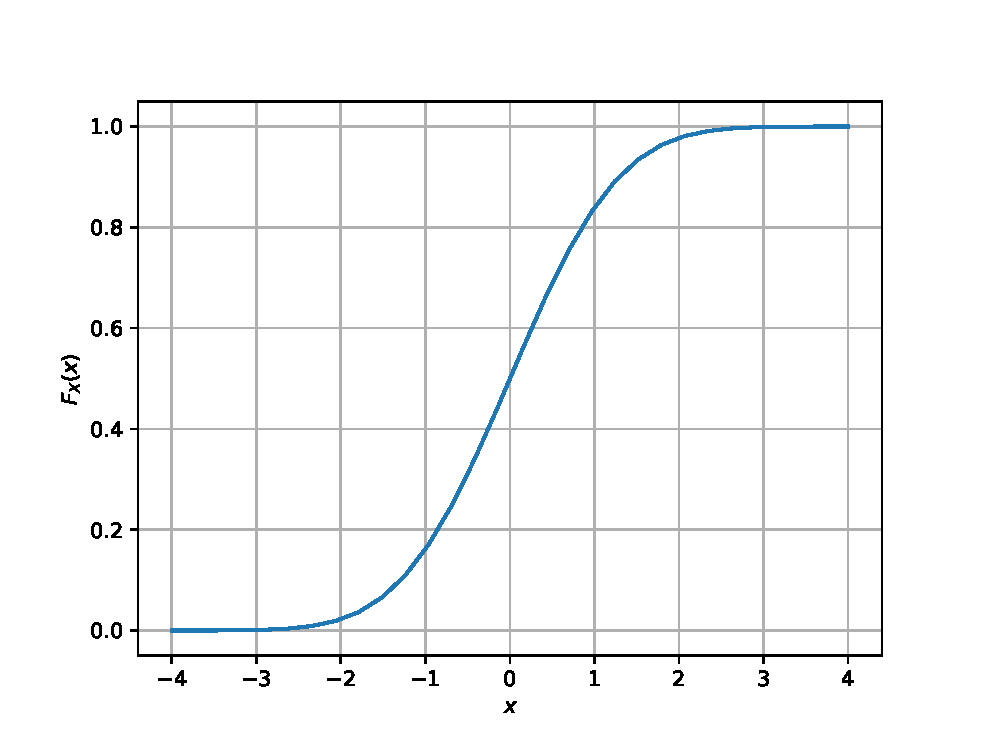
\includegraphics[width=\columnwidth]{./figs/gauss_cdf}
\caption{The CDF of $X$}
\label{fig:gauss_cdf}
\end{figure}
\item
Load gau.dat in python and plot the empirical PDF of $X$ using the samples in gau.dat. The PDF of $X$ is defined as
\begin{align}
p_{X}(x) = \frac{d}{dx}F_{X}(x)
\end{align}
What properties does the PDF have?
\\
\solution The PDF of $X$ is plotted in Fig. \ref{fig:gauss_pdf} using the code below
\begin{lstlisting}
codes/pdf_plot.py
\end{lstlisting}

\begin{figure}
\centering
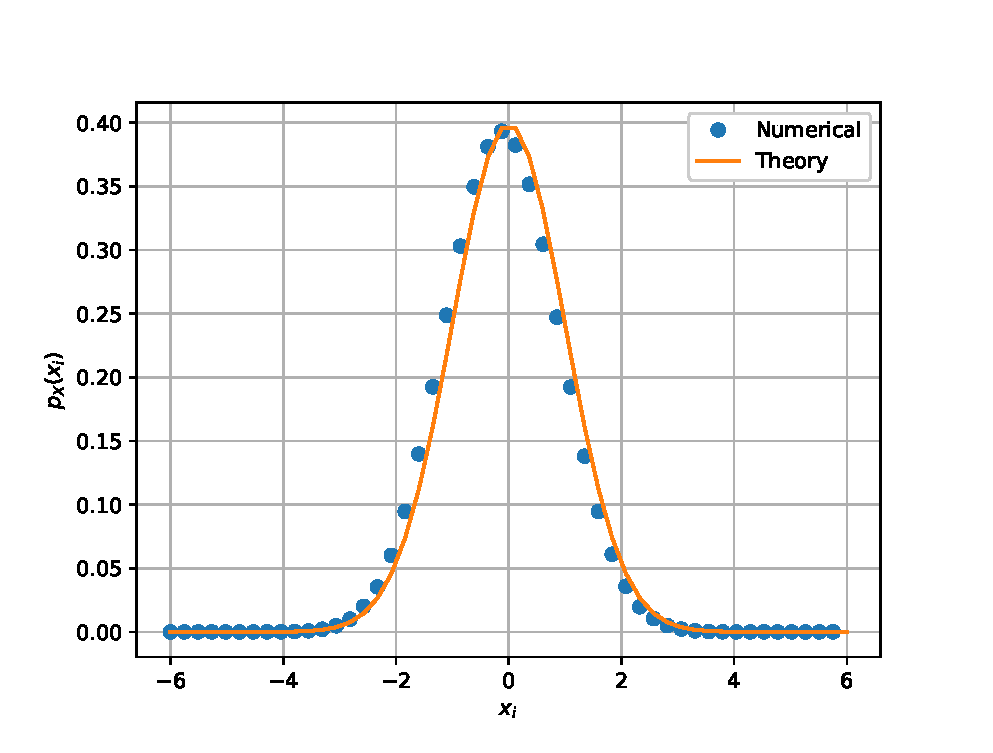
\includegraphics[width=\columnwidth]{./figs/gauss_pdf}
\caption{The PDF of $X$}
\label{fig:gauss_pdf}
\end{figure}

\item Find the mean and variance of $X$ by writing a C program.
\item Given that 
\begin{align}
p_{X}(x) = \frac{1}{\sqrt{2\pi}}\exp\brak{-\frac{x^2}{2}}, -\infty < x < \infty,
\end{align}
repeat the above exercise theoretically.
%
\end{enumerate}
\section{From Uniform to Other}
\begin{enumerate}[label=\thesection.\arabic*
,ref=\thesection.\theenumi]
%
\item
Generate samples of 
%
\begin{equation}
V = -2\ln\brak{1-U}
\end{equation}
%
and plot its CDF.  
\item Find a theoretical expression for $F_V(x)$.

%
%\item
%Generate the Rayleigh distribution from Uniform. Verify your result through graphical plots.
\end{enumerate}

\section{Triangular Distribution}
\begin{enumerate}[label=\thesection.\arabic*
,ref=\thesection.\theenumi]
%
\item Generate 
	\begin{align}
		T = U_1+U_2
	\end{align}
\item Find the CDF of $T$.
\item Find the PDF of $T$.
\item Find the theoretical expressions for the PDF and CDF of $T$.
\item Verify your results through a plot. 
\end{enumerate}
\section{Maximum Likelihood}
\begin{enumerate}[label=\thesection.\arabic*
,ref=\thesection.\theenumi]
\item Generate equiprobable $X \in \cbrak{1,-1}$.
\item Generate 
\begin{equation}
Y = AX+N,
\end{equation}
		where $A = 5$ dB,  and $N \sim \gauss{0}{1}$.
	\item Plot $Y$ using a scatter plot.
	\item Guess how to estimate $X$ from $Y$.
\item
\label{ml-ch4_sim}
Find 
\begin{equation}
	P_{e|0} = \pr{\hat{X} = -1|X=1}
\end{equation}
and 
\begin{equation}
	P_{e|1} = \pr{\hat{X} = 1|X=-1}
\end{equation}
%
\item Find $P_e$ assuming that $X$ has equiprobable symbols.

%
\item
Verify by plotting  the theoretical $P_e$ with respect to $A$ from 0 to 10 dB.  
%
\item Now, consider a threshold $\delta$  while estimating $X$ from $Y$. Find the value of $\delta$ that maximizes the theoretical $P_e$.
\item Repeat the above exercise when 
	\begin{align}
		p_{X}(0) = p
	\end{align}
\item Repeat the above exercise using the MAP criterion.

		\end{enumerate}
		\fi
\section{Gaussian to Other}
\begin{enumerate}[label=\thesection.\arabic*
,ref=\thesection.\theenumi]
\item
Let $X_1 \sim  \gauss{0}{1}$ and $X_2 \sim  \gauss{0}{1}$. Plot the CDF and PDF of
%
\begin{equation}
V = X_1^2 + X_2^2
\end{equation}
%

%
%
\item
If
%
\begin{equation}
F_{V}(x) = 
\begin{cases}
1 - e^{-\alpha x} & x \geq 0 \\
0 & x < 0,
\end{cases}
\end{equation}
%
find $\alpha$.

%
\item
\label{ch3_raleigh_sim}
Plot the CDF and PDf of
%
\begin{equation}
A = \sqrt{V}
\end{equation}
%


\end{enumerate}

\section{Conditional Probability}
\begin{enumerate}[label=\thesection.\arabic*
,ref=\thesection.\theenumi]
\item
\label{ch4_sim}
Plot 
\begin{equation}
P_e = \pr{\hat{X} = -1|X=1}
\end{equation}
%
for 
\begin{equation}
Y = AX+N,
\end{equation}
where $A$ is Raleigh with $E\sbrak{A^2} = \gamma, N \sim \gauss{0}{1}, X \in \brak{-1,1}$ for $0 \le \gamma \le 10$ dB.

%
\item
Assuming that $N$ is a constant, find an expression for $P_e$.  Call this $P_e(N)$

%
\item
%
\label{ch4_anal}
For a function $g$,
\begin{equation}
E\sbrak{g(X)} = \int_{-\infty}^{\infty}g(x)p_{X}(x)\, dx
\end{equation}
%
Find $P_e = E\sbrak{P_e(N)}$.

%
\item
Plot $P_e$ in problems \ref{ch4_sim} and \ref{ch4_anal} on the same graph w.r.t $\gamma$.  Comment.

		\end{enumerate}
		\iffalse
\section{Two Dimensions}
Let 
\begin{equation}
\mbf{y} = A\mbf{x} + \mbf{n},
\end{equation}
where 
\begin{align}
x &\in \brak{\mbf{s}_0,\mbf{s}_1}, 
\mbf{s}_0 = 
\begin{pmatrix}
1 
\\
0
\end{pmatrix},
\mbf{s}_1 = 
\begin{pmatrix}
0 
\\
1
\end{pmatrix}
\\
\mbf{n} &= 
\begin{pmatrix}
n_1
\\
n_2
\end{pmatrix},
n_1,n_2 \sim \gauss{0}{1}.
\end{align}
%
\begin{enumerate}[label=\thesection.\arabic*
,ref=\thesection.\theenumi]

%%
\item
\label{ch5_fsk}
Plot 
%
\begin{equation}
\mbf{y}|\mbf{s}_0 \text{ and } \mbf{y}|\mbf{s}_1
\end{equation}
%
on the same graph using a scatter plot.

%
\item
For the above problem, find a decision rule for detecting the symbols $\mbf{s}_0 $ and $\mbf{s}_1$.

%
\item
Plot 
\begin{equation} 
P_e = \pr{\hat{\mbf{x}} = \mbf{s}_1|\mbf{x} = \mbf{s}_0}
\end{equation}
with respect to the SNR from 0 to 10 dB.

%
\item
Obtain an expression for $P_e$. Verify this by comparing the theory and simulation plots on the same graph.

%
		\end{enumerate}
\end{document}
\fi

\chapter{Bivariate Random Variables: FSK}
\input{probability/bivar.tex}
\chapter{Exercises}
\iffalse
\documentclass[journal,12pt,twocolumn]{IEEEtran}
%
\usepackage{setspace}
\usepackage{gensymb}
\usepackage{xcolor}
\usepackage{caption}
%\usepackage{subcaption}
%\doublespacing
\singlespacing
\usepackage{multicol}

\usepackage{iithtlc}
%\usepackage{graphicx}
%\usepackage{amssymb}
%\usepackage{relsize}
\usepackage[cmex10]{amsmath}
\usepackage{mathtools}
%\usepackage{amsthm}
%\interdisplaylinepenalty=2500
%\savesymbol{iint}
%\usepackage{txfonts}
%\restoresymbol{TXF}{iint}
%\usepackage{wasysym}
\usepackage{amsthm}
\usepackage{mathrsfs}
\usepackage{txfonts}
\usepackage{stfloats}
\usepackage{cite}
\usepackage{cases}
\usepackage{subfig}
%\usepackage{xtab}
\usepackage{longtable}
\usepackage{multirow}
%\usepackage{algorithm}
%\usepackage{algpseudocode}
\usepackage{enumitem}
\usepackage{mathtools}
%\usepackage{stmaryrd}

\usepackage{listings}
    \usepackage[latin1]{inputenc}                                 %%
    \usepackage{color}                                            %%
    \usepackage{array}                                            %%
    \usepackage{longtable}                                        %%
    \usepackage{calc}                                             %%
    \usepackage{multirow}                                         %%
    \usepackage{hhline}                                           %%
    \usepackage{ifthen}                                           %%
  %optionally (for landscape tables embedded in another document): %%
    \usepackage{lscape}     

%\usepackage{wasysym}
%\newcounter{MYtempeqncnt}
\DeclareMathOperator*{\Res}{Res}
%\renewcommand{\baselinestretch}{2}
\renewcommand\thesection{\arabic{section}}
\renewcommand\thesubsection{\thesection.\arabic{subsection}}
\renewcommand\thesubsubsection{\thesubsection.\arabic{subsubsection}}

\renewcommand\thesectiondis{\arabic{section}}
\renewcommand\thesubsectiondis{\thesectiondis.\arabic{subsection}}
\renewcommand\thesubsubsectiondis{\thesubsectiondis.\arabic{subsubsection}}

% correct bad hyphenation here
\hyphenation{op-tical net-works semi-conduc-tor}

\def\inputGnumericTable{}  

\lstset{
language=python,
frame=single, 
breaklines=true
}

\begin{document}
%

\theoremstyle{definition}

\newtheorem{theorem}{Theorem}[section]
\newtheorem{problem}{Problem}
\newtheorem{proposition}{Proposition}[section]
\newtheorem{lemma}{Lemma}[section]
\newtheorem{corollary}[theorem]{Corollary}
\newtheorem{example}{Example}[section]
\newtheorem{definition}{Definition}[section]
%\newtheorem{algorithm}{Algorithm}[section]
%\newtheorem{cor}{Corollary}
\newcommand{\BEQA}{\begin{eqnarray}}
\newcommand{\EEQA}{\end{eqnarray}}
\newcommand{\triangleq}{\stackrel{\triangle}{=}}

\bibliographystyle{IEEEtran}
%\bibliographystyle{ieeetr}



\providecommand{\pr}[1]{\ensuremath{\Pr\left(#1\right)}}
\providecommand{\qfunc}[1]{\ensuremath{Q\left(#1\right)}}
\providecommand{\sbrak}[1]{\ensuremath{{}\left[#1\right]}}
\providecommand{\lsbrak}[1]{\ensuremath{{}\left[#1\right.}}
\providecommand{\rsbrak}[1]{\ensuremath{{}\left.#1\right]}}
\providecommand{\brak}[1]{\ensuremath{\left(#1\right)}}
\providecommand{\lbrak}[1]{\ensuremath{\left(#1\right.}}
\providecommand{\rbrak}[1]{\ensuremath{\left.#1\right)}}
\providecommand{\cbrak}[1]{\ensuremath{\left\{#1\right\}}}
\providecommand{\lcbrak}[1]{\ensuremath{\left\{#1\right.}}
\providecommand{\rcbrak}[1]{\ensuremath{\left.#1\right\}}}
\theoremstyle{remark}
\newtheorem{rem}{Remark}
\newcommand{\sgn}{\mathop{\mathrm{sgn}}}
\providecommand{\abs}[1]{\left\vert#1\right\vert}
\providecommand{\res}[1]{\Res\displaylimits_{#1}} 
\providecommand{\norm}[1]{\lVert#1\rVert}
\providecommand{\mtx}[1]{\mathbf{#1}}
\providecommand{\mean}[1]{E\left[ #1 \right]}
\providecommand{\fourier}{\overset{\mathcal{F}}{ \rightleftharpoons}}
%\providecommand{\hilbert}{\overset{\mathcal{H}}{ \rightleftharpoons}}
\providecommand{\system}{\overset{\mathcal{H}}{ \longleftrightarrow}}
\providecommand{\gauss}[2]{\mathcal{N}\ensuremath{\left(#1,#2\right)}}
	%\newcommand{\solution}[2]{\textbf{Solution:}{#1}}
\newcommand{\solution}{\noindent \textbf{Solution: }}
\providecommand{\dec}[2]{\ensuremath{\overset{#1}{\underset{#2}{\gtrless}}}}
%\numberwithin{equation}{section}
%\numberwithin{problem}{section}

\def\putbox#1#2#3{\makebox[0in][l]{\makebox[#1][l]{}\raisebox{\baselineskip}[0in][0in]{\raisebox{#2}[0in][0in]{#3}}}}
     \def\rightbox#1{\makebox[0in][r]{#1}}
     \def\centbox#1{\makebox[0in]{#1}}
     \def\topbox#1{\raisebox{-\baselineskip}[0in][0in]{#1}}
     \def\midbox#1{\raisebox{-0.5\baselineskip}[0in][0in]{#1}}


% paper title
% can use linebreaks \\ within to get better formatting as desired
\title{
%\logo{
Digital Modulation Techniques
%}
}
%
%
% author names and IEEE memberships
% note positions of commas and nonbreaking spaces ( ~ ) LaTeX will not break
% a structure at a ~ so this keeps an author's name from being broken across
% two lines.
% use \thanks{} to gain access to the first footnote area
% a separate \thanks must be used for each paragraph as LaTeX2e's \thanks
% was not built to handle multiple paragraphs
%

%\author{Y Aditya, A Rathnakar and G V V Sharma$^{*}$% <-this % stops a space
\author{P.~N.~V.~S.~S.~K.~ HAVISH, S.~S.~Ashish and G V V Sharma %<-this  stops a space
\thanks{The authors are with the Department
of Electrical Engineering, IIT, Hyderabad
502285 India e-mail: \{ee16btech11023,ee16btech11043,jbala,gadepall\}@iith.ac.in. All material in the manuscript is released under GNU GPL.  Free to use for all.
}}



% make the title area
\maketitle

\tableofcontents

\bigskip

\begin{abstract}
%\boldmath
The manual frames the problems of receiver design and performance analysis in digital communication as applications of probability theory.

\end{abstract}
% IEEEtran.cls defaults to using nonbold math in the Abstract.
% This preserves the distinction between vectors and scalars. However,
% if the journal you are submitting to favors bold math in the abstract,
% then you can use LaTeX's standard command \boldmath at the very start
% of the abstract to achieve this. Many IEEE journals frown on math
% in the abstract anyway.

% Note that keywords are not normally used for peerreview papers.
%\begin{IEEEkeywords}
%Cooperative diversity, decode and forward, piecewise linear
%\end{IEEEkeywords}



% For peer review papers, you can put extra information on the cover
% page as needed:
% \ifCLASSOPTIONpeerreview
% \begin{center} \bfseries EDICS Category: 3-BBND \end{center}
% \fi
%
% For peerreview papers, this IEEEtran command inserts a page break and
% creates the second title. It will be ignored for other modes.
\IEEEpeerreviewmaketitle

\fi
\section{BPSK}
\begin{enumerate}
\item
The {\em signal constellation diagram} for BPSK is given by Fig. \ref{fig:bpsk_const}.  The symbols $s_0$ and $s_1$ are equiprobable.  $\sqrt{E_b}$ is the energy transmitted per bit. Assuming a zero mean additive white gaussian noise (AWGN) with variance $\frac{N_0}{2}$,
obtain the symbols that are received.

%
\begin{figure}[!h]
\centering
\includegraphics[width=\columnwidth]{./manual/figs/bpsk_const.eps}
\caption{}
\label{fig:bpsk_const}
\end{figure}
\solution The possible received symbols are
\begin{align}
y|s_0 &= \sqrt{E_b} + n
\\
y|s_1 &= -\sqrt{E_b} + n
\end{align}
%
where the AWGN $n \sim \gauss{0}{\frac{N_0}{2}}$.
%
\item
\label{prob:bpsk_decision}
From Fig. \ref{fig:bpsk_const} obtain a decision rule for BPSK

\solution The decision rule is
\begin{equation}
y \dec{s_0}{s_1} 0
\end{equation}
\item
Repeat the previous exercise using the MAP criterion.

\item
Using the decision rule in Problem \ref{prob:bpsk_decision}, obtain an expression for the probability of error for BPSK.

\solution
Since the symbols are equiprobable, it is sufficient if the error is calculated assuming that a 0 was sent.  This results in
\begin{align}
P_e &= \pr{y < 0|s_0} = \pr{\sqrt{E_b} + n < 0}
\\
&= \pr{ -n > \sqrt{E_b} } = \pr{ n > \sqrt{E_b} }
\label{eq:bpsk_proof_n0}
\end{align}
since $n$ has a symmetric pdf.
Let $w \sim \gauss{0}{1}$.  Then $n = \sqrt{\frac{N_0}{2}}w$. Substituting this in \eqref{eq:bpsk_proof_n0},
\begin{align}
P_e &=  \pr{ \sqrt{\frac{N_0}{2}}w > \sqrt{E_b} } = \pr{ w > \sqrt{\frac{2E_b}{N_0}} }
\\
&= \qfunc{\sqrt{\frac{2E_b}{N_0}}}
\end{align}
%
where $\qfunc{x} \triangleq \pr{w > x}, x \ge 0$.
\item
The PDF of $w \sim \gauss{0}{1}$ is given by
%
\begin{equation}
p_{w}(x) = \frac{1}{\sqrt{2\pi}}\exp\brak{-\frac{x^2}{2}}, -\infty < x < \infty
\end{equation}
and the complementary error function is defined as
\begin{equation}
\operatorname {erfc} (x)={\frac {2}{\sqrt {\pi }}}\int _{x}^{\infty }e^{-t^{2}}\,dt.
\end{equation}
%
Show that 
\begin{equation}
Q(x) = \frac{1}{2}\operatorname {erfc}\left({\frac  {x}{{\sqrt  {2}}}}\right)
\end{equation}

\item
Verify the bit error rate (BER) plots for BPSK through simulation and analysis for 0 to 10 dB.

\solution
The following code
%\lstinputlisting{./codes/bpsk_ber.py}
%\iffalse
\begin{lstlisting}
codes/bpsk_ber.py
\end{lstlisting}
%	\fi
yields Fig. \ref{fig:bpsk_ber}
\begin{figure}[!h]
\centering
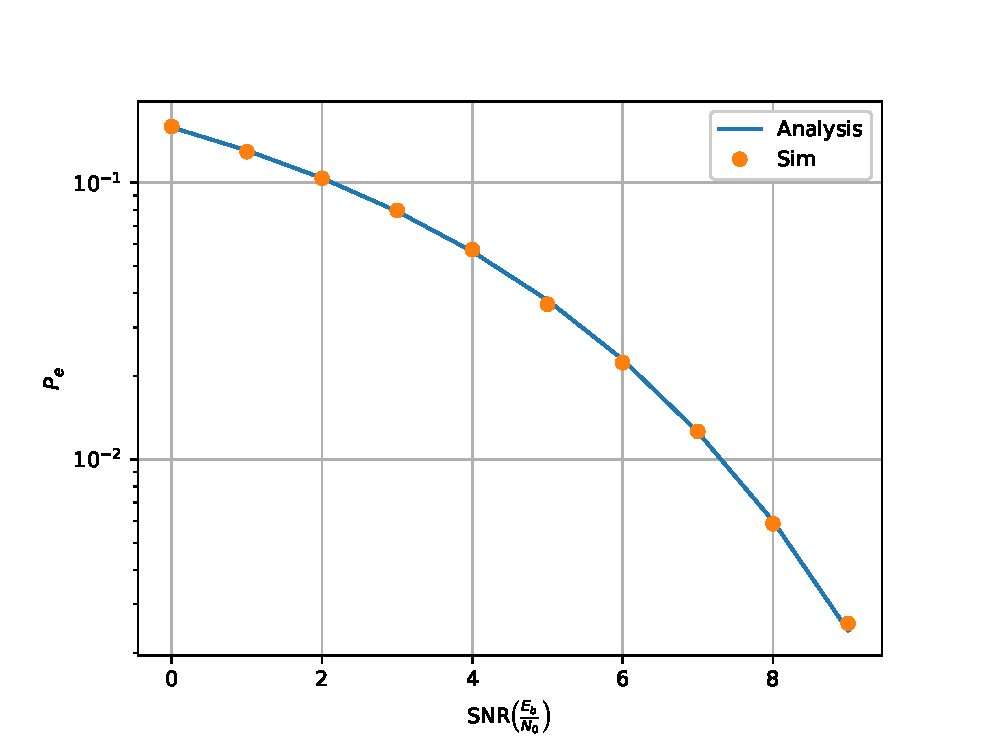
\includegraphics[width=\columnwidth]{./manual/figs/bpsk_ber.eps}
\caption{}
\label{fig:bpsk_ber}
\end{figure}

\item
Show that
\begin{equation}
Q(x) = \frac{1}{\pi}\int^{\frac{\pi}{2}}_{0}e^{-\frac{x^2}{2\sin^2 \theta}}\,d\theta
\end{equation}
\end{enumerate}
\section{Coherent BFSK}
\begin{enumerate}
\item
The signal constellation for binary frequency shift keying (BFSK) is given in Fig. \ref{fig:bfsk_const}.
Obtain the equations for the received symbols.

\begin{figure}[!h]
\centering
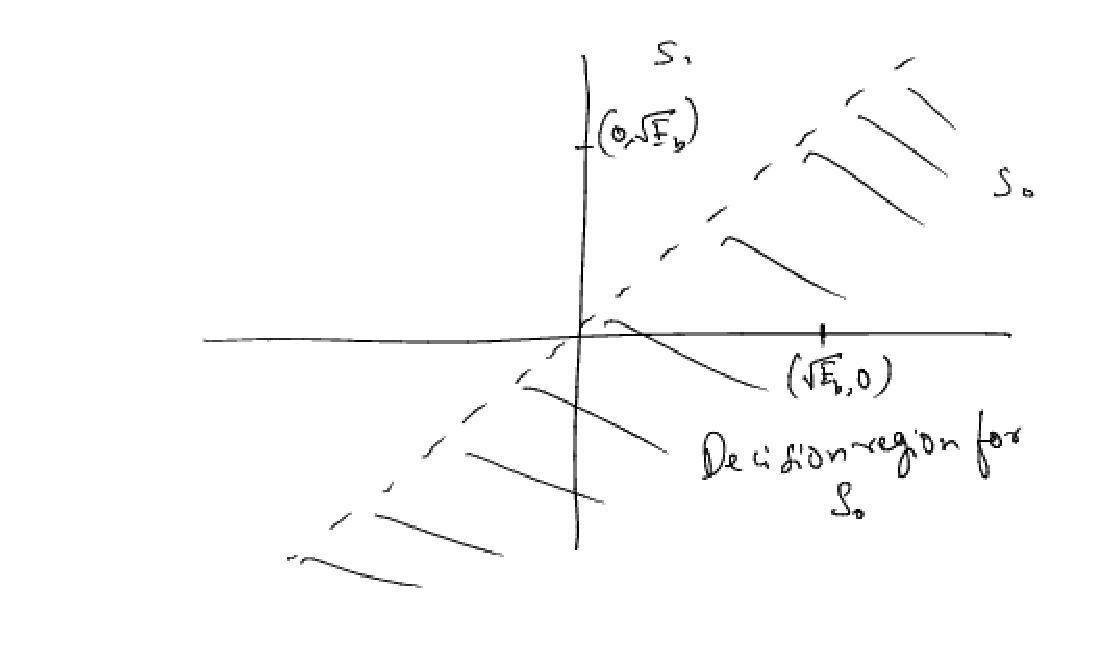
\includegraphics[width=\columnwidth]{./manual/figs/bfsk_const.eps}
\caption{}
\label{fig:bfsk_const}
\end{figure}
\solution
The received symbols are given by
\begin{align}
\mathbf{y}|s_0 = 
\myvec{
\sqrt{E_b} \\
0
}
+
\myvec{
 n_{1}\\
n_{2}
},
\end{align}
and 
\begin{align}
\mathbf{y}|s_1 = 
\myvec{
0\\
\sqrt{E_b} 
}
+
\myvec{
n_{1}\\
 n_{2}
},
\end{align}
where $n_1,n_2 \sim \gauss{0}{\frac{N_0}{2}}$. and
$
\mathbf{y} = 
\myvec{
y_{1}\\
 y_{2}
}
$.
\item
Obtain a decision rule for BFSK from Fig. \ref{fig:bfsk_const}.

\solution The decision rule is
\begin{equation}
y_1 \dec{s_0}{s_1} y_2
\end{equation}
\item
Repeat the previous exercise using the MAP criterion.

\item
Derive and plot the probability of error.  Verify through simulation.
\end{enumerate}

%
\section{QPSK}
\begin{enumerate}
\item
Let
\begin{equation}
\mathbf{r} = \mathbf{s}+ \mathbf{n}
\end{equation}
where $\mathbf{s} \in \cbrak{s_0,s_1,s_2, s_3}$ and
\begin{align}
\mathbf{s}_0 &= 
\myvec{
\sqrt{E_b}\\
0
},
\mathbf{s}_1 = 
\myvec{
0\\
\sqrt{E_b}
},
\\
\mathbf{s}_2 &= 
\myvec{
-\sqrt{E_b}\\
0
},
\mathbf{s}_3 = 
\myvec{
0\\
-\sqrt{E_b}
},
\\
E\sbrak{\mathbf{n}} &= \mathbf{0}, E\sbrak{\mathbf{n}\mathbf{n}^T} = \sigma^2 \mathbf{I}
\end{align}
%
\begin{enumerate}
\item Show that the MAP decision for detecting $\mathbf{s}_0$ results in
\begin{equation}
\abs{r}_2 < r_1
\end{equation}
\item Express $\pr{\hat{\mathbf{s}} = \mathbf{s}_0|\mathbf{s} = \mathbf{s}_0}$ in terms of $r_1, r_2$.
Let $X=n_2-n_1, Y = -n_2-n_1$, where $\mathbf{n}=\brak{n_1,n_2}$.
Their correlation coefficient is defined as
%
\begin{align}
\rho = \frac{E\sbrak{\brak{X-\mu_x}\brak{Y-\mu_y}}}{\sigma_x\sigma_y}
\end{align}
%
$X$ and $Y$ are said to be uncorrelated if $\rho = 0$
\item Show that if $X$ and $Y$ are uncorrelated 
Verify this numerically.
\item Show that $X$ and $Y$ are independent, i.e. $p_{XY}(x,y) = p_{X}(x)p_{Y}(y)$.
\item Show that $X,Y \sim \mathcal{N}\brak{0,2\sigma^2}$.
\item Show that $\pr{\hat{\mathbf{s}} = \mathbf{s}_0|\mathbf{s} = \mathbf{s}_0} =\pr{ X < A,  Y < A}$.
\item Find $\pr{ X < A,  Y < A}$.
\item Verify the above through simulation.
\end{enumerate}
\end{enumerate}

\section{$M$-PSK}
\begin{enumerate}

\item
Consider a system where 
$\mathbf{s}_i=
\myvec{
\cos\brak{\frac{2\pi i}{M}}\\
\cos\brak{\frac{2\pi i}{M}}
}, i = 0, 1 , \dots M-1
$
.
Let
%
\begin{align}
\mathbf{r}|s_0 = 
\myvec{
r_1\\
r_2
}
=
\myvec{
\sqrt{E_s}+n_1\\
n_2
}
\end{align}
where $n_1,n_2 \sim \mathcal{N}\brak{0,\frac{N_0}{2}}$.

\begin{enumerate}
\item Substituting 
\begin{align}
r_1=R\cos \theta \\
r_2=R\sin \theta
\end{align}
show that the joint pdf of $R,\theta$ is
%
\begin{equation}
p\brak{R,\theta}=\frac{R}{\pi N_0}\exp\brak{-\frac{R^2-2R\sqrt{E_s}\cos \theta + E_s}{N_0}}
\end{equation}
%
\item Show that 
%
\begin{align}
\lim_{\alpha \rightarrow \infty}\int_{0}^{\infty}\brak{V-\alpha }e^{-\brak{V-\alpha}^2 }\,dV
&= 0
\\
\lim_{\alpha \rightarrow \infty}\int_{0}^{\infty} e^{-\brak{V-\alpha}^2 }\,dV
&=  \sqrt{\pi}
\end{align}
%
\item 
Using the above, evaluate
%
\begin{align}
\int_{0}^{\infty}V\exp\cbrak{-\brak{V^2 - 2V \sqrt{\gamma}\cos \theta +\gamma}}\,dV
\end{align}
%
for large values of $\gamma$.
\item
Find a compact expression for 
%
\begin{align}
I = 1 - \sqrt{\frac{\gamma}{\pi}}\int_{-\frac{\pi}{M}}^{\frac{\pi}{M}}e^{- \gamma\sin^2\theta }\cos \theta\, d\theta
\end{align}
\item Find $P_{e|\mathbf{s}_0}$.
\end{enumerate}
\end{enumerate}
\section{Noncoherent BFSK}
\begin{enumerate}[label=\thesection.\arabic*
,ref=\thesection.\theenumi]
\item
Show that
%
\begin{align}
I_{0}(x) &= \frac{1}{2\pi}\int_{0}^{2\pi}e^{x\cos\theta}\,d\theta \\
I_{0}(x) &= \frac{1}{2\pi}\int_{0}^{2\pi}e^{x\cos\brak{\theta-\phi}}\,d\theta \\
\frac{1}{2\pi}\int_{0}^{2\pi}e^{m_1\cos\theta + m_2\sin\theta}\,d\theta &= I_0\brak{\sqrt{m_1^2+m_2^2}} 
\end{align}
%
where the modified Bessel function of order $n$ (integer) is defined as 
%
\begin{align}
I_{n}(x) = \frac{1}{\pi}\int_{0}^{\pi}e^{x\cos\theta}\cos n\theta\,d\theta
\end{align}
\item
Let
%
\begin{align}
\mathbf{r}|0= \sqrt{E_b}
\myvec{
\cos \phi_0\\
\sin \phi_0 \\
0\\
0
}
+\mathbf{n}_0,
\mathbf{r}|1= \sqrt{E_b}
\myvec{
0\\
0 \\
\cos \phi_1\\
\sin \phi_1 
}
+\mathbf{n}_1
\end{align}
%
where $\mathbf{n}_0,\mathbf{n}_1\sim \mathcal{N}\brak{\mathbf{0}, \frac{N_0}{2}\mathbf{I}}$.
%
\begin{enumerate}
\item Taking $\mathbf{r} = \brak{r_1,r_2,r_3,r_4}^{T},$, find the pdf $p\brak{\mathbf{r}|0,\phi_0}$ in
terms of $r_1,r_2,r_3,r_4,\phi,E_b$ and $N_0$. Assume that all noise variables are independent.
%
\item 
If $\phi_0$ is uniformly distributed between 0 and $2\pi$, find $p\brak{\mathbf{r}|0}$.  Note that this expression will no longer contain $\phi_0$.
%
\item
Show that the ML detection criterion for this scheme is
%
\begin{align}
I_0\brak{k\sqrt{r_1^2+r_2^2}}\dec{0}{1}I_0\brak{k\sqrt{r_3^2+r_4^2}}
\end{align}
%
where $k$ is a constant.
%
\item 
The above criterion reduces to something simpler.  Can you guess what it is?  Justify your answer.
%
\item 
Show that 
%
\begin{align}
P_{e|0}=\pr{r_1^2+r_2^2 < r_3^2+r_4^2 | 0}
\end{align}
%
\item 
Show that the pdf of $Y=r_3^2+r_4^2$ id
%
\begin{align}
p_{Y}(y) = \frac{1}{N_0}e^{-\frac{y}{N_0}}, y > 0
\end{align}
%
\item 
Find 
%
\begin{align}
g\brak{r_1,r_2} = \pr{r_1^2+r_2^2<Y|0,r_1,r_2}.
\end{align}
\item 
Show that $E\sbrak{e^{-\frac{X^2}{2\sigma^2}}}=\frac{1}{\sqrt{2}}e^{-\frac{\mu^2}{4\sigma^2}}$ for $X \sim 
\mathcal{N}\brak{\mu,\sigma^2}$.
%
\item 
Now show that
%
\begin{align}
E\sbrak{g\brak{r_1,r_2}}=\frac{1}{2}e^{-\frac{E_b}{2N_0}}.
\end{align}
%
\end{enumerate}
\item
 Let $U,V\sim\mathcal{N}\brak{0,\frac{k}{2}}$ be i.i.d.  Assuming that
%
\begin{align}
U = \sqrt{R} \cos \Theta \\
V = \sqrt{R} \sin \Theta
\end{align}
\begin{enumerate}
\item 
Compute the jacobian for $U,V$ with respect to $X$ and $\Theta$ defined by
%
\begin{align}
J = \det\brak{
\begin{matrix}
\frac{\partial U}{\partial R} & \frac{\partial U}{\partial \Theta} \\
\frac{\partial V}{\partial R} & \frac{\partial V}{\partial \Theta}
\end{matrix}
}
\end{align}
\item 
The joint pdf for $R,\Theta$ is given by,
%
\begin{align}
p_{R,\Theta}\brak{r,\theta} = p_{U,V}\brak{u,v}J\vert_{u = \sqrt{r}\cos\theta,v = \sqrt{r}\sin\theta}
\end{align}
%
Show that
%
\begin{align}
p_{R}(r) = 
\begin{cases}
\frac{1}{k}e^{-\frac{r}{k}} & r > 0, \\
0 & r < 0,
\end{cases}
\end{align}
%
assuming that $\Theta$ is uniformly distributed between 0 to $2\pi$.
\item
Show that the pdf of $Y = R_1-R_2$, where $R_1$ and $R_2$ are i.i.d. and have the same distribution as $R$ is
%
\begin{align}
p_{Y}(y) = \frac{1}{2k}e^{-\frac{\abs{y}}{k}}
\end{align}
%
\item 
 Find the pdf of 
%
\begin{align}
Z = p + \sqrt{p}\sbrak{U \cos \phi + V \sin \phi}
\end{align}
%
where $\phi$ is a constant.
\item 
Find $\pr{Y > Z}$.
\item 
If $U\sim\mathcal{N}\brak{m_1,\frac{k}{2}},V\sim\mathcal{N}\brak{m_2,\frac{k}{2}}$, where $m_1,m_2, k$ are constants, show that the pdf of 
%
\begin{align}
R = \sqrt{U^2+V^2}
\end{align}
%
is
%
\begin{align}
p_{R}\brak{r} = \frac{e^{-\frac{r +m}{k}}}{ k}I_{0}\brak{\frac{2\sqrt{mr}}{k}},\quad m = \sqrt{m_1^2+m_2^2}
\end{align}
%
\item
Show that
\begin{align}
I_0(x) = \sum_{n=0}^{\infty}\frac{x^{2n}}{4^n\brak{n!}^2}
\end{align}
\item 
If
%
\begin{align}
p_{Z}(z) &= 
\begin{cases}
\frac{1}{k} e^{-\frac{z}{k}} & z \geq 0 \\
0 & z < 0
\end{cases}
\end{align}
%
find $\pr{R < Z}$.
\end{enumerate}
\end{enumerate}
\section{Craig's Formula and MGF}
\begin{enumerate}[label=\thesection.\arabic*
,ref=\thesection.\theenumi]
\item
The Moment Generating Function (MGF) of $X$ is defined as
%
\begin{align}
M_{X}(s) = E\sbrak{e^{s X}}
\end{align}
%
where $X$ is a random variable and $E\sbrak{\cdot}$ is the expectation.  
%
%
\begin{enumerate}
\item Let $Y \sim \gauss{0}{1}$.  Define
%
\begin{align}
Q(x) = \pr{Y > x}, x > 0
\end{align}
%
Show that
\begin{equation}
Q(x) = \frac{1}{\pi}\int^{\frac{\pi}{2}}_{0}e^{-\frac{x^2}{2\sin^2 \theta}}\,d\theta
\end{equation}
\item 
Let $h\sim\mathcal{CN}\brak{0,\frac{\Omega}{2}},n\sim\mathcal{CN}\brak{0,\frac{N_0}{2}}$.  Find the distribution of $\abs{h}^2$.
\item Let
%
\begin{align}
P_e = \pr{\Re \cbrak{h^*y} < 0}, \text{ where } y = \brak{\sqrt{E_s}h + n},
\end{align}
%
Show that
%
\begin{align}
P_e = \int_{0}^{\infty}\qfunc{\sqrt{2x}}p_{A}(x) \,dx
\end{align}
where $A = \frac{E_s\abs{h}^2}{N_0}$.
\item Show that
%
\begin{align}
P_e 
%&= E\sbrak{\qfunc{\sqrt{2A}}} \\
%&=  \frac{1}{\pi}\int_{0}^{\frac{\pi}{2}}E\sbrak{e^{-\frac{A}{\sin^2\theta}}}\,d\theta \\
&=  \frac{1}{\pi}\int_{0}^{\frac{\pi}{2}}M_{A}\brak{-\frac{1}{\sin^2\theta}}\,d\theta
\label{ch4_pe_mgf}
\end{align}
%
\item compute $M_A(s)$.
%
\item 
Find $P_e$.
\item 
If $\gamma = \frac{\Omega E_s}{N_0}$, show that $P_e < \frac{1}{2\gamma}$. 
\end{enumerate}
\end{enumerate}
%







\chapter{Random Processes}
\begin{enumerate}[label=\thechapter.\arabic*,ref=\thechapter.\theenumi]
\item The frequency response $H(f)$ of of a linear time-invariant syatem has magnitude as shown in \figref{fig:23,2022}\\
Statement 1: The system is necessarily a pure delay system for inputs which are bandlimited to $-a \leq f \leq a$.\\
Statement 2: For any wide-sense stationary input process with power spectral density $S_X(f)$, the output power spectral density $S_Y(f)$ obeys $S_X(f)=S_Y(f)$ for $-a \leq f \leq a$.
\hfill (GATE EC 2022)\\
\begin{figure}[!ht]
\centering
\includegraphics[width=\columnwidth]{gate/EC/2022/23/figs/figure.png}
\caption{$|H(f)|$ vs frequency}
\label{fig:23,2022}
\end{figure}
\iffalse
\let\negmedspace\undefined
\let\negthickspace\undefined
\documentclass[journal,12pt,twocolumn]{IEEEtran}
\usepackage{cite}
\usepackage{amsmath,amssymb,amsfonts,amsthm}
\usepackage{algorithmic}
\usepackage{graphicx}
\usepackage{textcomp}
\usepackage{xcolor}
\usepackage{txfonts}
\usepackage{listings}
\usepackage{enumitem}
\usepackage{mathtools}
\usepackage{gensymb}
\usepackage{comment}
\usepackage[breaklinks=true]{hyperref}
\usepackage{tkz-euclide} 
\usepackage{listings}
\usepackage{gvv}                                        
\def\inputGnumericTable{}                                 
\usepackage[latin1]{inputenc}                                
\usepackage{color}                                            
\usepackage{array}                                            
\usepackage{longtable}                                       
\usepackage{calc}                                             
\usepackage{multirow}                                         
\usepackage{hhline}                                           
\usepackage{ifthen}                                           
\usepackage{lscape}

\newtheorem{theorem}{Theorem}[section]
\newtheorem{problem}{Problem}
\newtheorem{proposition}{Proposition}[section]
\newtheorem{lemma}{Lemma}[section]
\newtheorem{corollary}[theorem]{Corollary}
\newtheorem{example}{Example}[section]
\newtheorem{definition}[problem]{Definition}
\newcommand{\BEQA}{\begin{eqnarray}}
\newcommand{\EEQA}{\end{eqnarray}}
\newcommand{\define}{\stackrel{\triangle}{=}}
\theoremstyle{remark}
\newtheorem{rem}{Remark}
\begin{document}

\bibliographystyle{IEEEtran}
\vspace{3cm}

\title{Probability Assignment}
\author{EE22BTECH11022-G.SAI HARSHITH$^{*}$% <-this % stops a space
}
\maketitle
\newpage
\bigskip
\renewcommand{\thefigure}{\theenumi}
\renewcommand{\thetable}{\theenumi}

Question: The frequency response $H(f)$ of of a linear time-invariant syatem has magnitude as shown in \figref{fig:11}\\
Statement 1: The system is necessarily a pure delay system for inputs which are bandlimited to $-a \leq f \leq a$.\\
Statement 2: For any wide-sense stationary input process with power spectral density $S_X(f)$, the output power spectral density $S_Y(f)$ obeys $S_X(f)=S_Y(f)$ for $-a \leq f \leq a$.\\
\begin{figure}[!ht]
\centering
\includegraphics[width=\columnwidth]{figs/figure.png}
\caption{$|H(f)|$ vs frequency}
\label{fig:11}
\end{figure}\\
\fi
\solution A system where output signal is a delayed version of input signal with no other transformations or operations is called a pure delay system.
\begin{enumerate}
\item Let us consider a LTI system with x(t) and y(t) as input and output signal. Let $T_d$ be delay between input and output. So,
\begin{align}
y(t)&=x(t-T_d)
\end{align}
Here $Y(f)$ and $X(f)$ are output and input signals in frequency domian. Let $H(f)$ be 
\begin{align}
H(f)&=\frac{Y(f)}{X(f)}\\
&=e^{-2\pi fjT_d}\\
\label{eq:23.2022,2}
|H(f)|&=1\\
\angle H(f)&=-2\pi fT_d
\end{align}
The system will acts as pure delay system for frequency $f$. Now, if we take $f^2$ as frequency, the system doesn't act as pure delay system.\\
Example : Consider 
\begin{align}
H(f)=e^{-2\pi f^2jT_d}
\end{align}
Appling inverse fourier transform to get time responce.
\begin{align}
h(t)&=\int_{-\infty}^{\infty}H(f)e^{2\pi jft}df\\
&=\sqrt{\frac{T_d}{it}}e^{-\brak{\frac{i\pi t}{T_d}}} \ne \delta(t-T_d)
\end{align}
Therfore system doesn't necessarily be pure delay.
So, Statement 1 is incorrect.
\item For wide-sense stationary LTI sytem, Spectral power density of a signal describes the power present in the signal as a function of frequency, per unit frequency. In frequency domain,
\begin{align}
S_X(f)&=|X(f)|^2
\label{eq:23.2022,9}\\
S_Y(f)&=|Y(f)|^2
\label{eq:23.2022,10}
\end{align}
Dividing \eqref{eq:23.2022,9} and \eqref{eq:23.2022,10}.
\begin{align}
S_Y(f)&=\left|\frac{Y(f)}{X(f)}\right|^2S_X(f)\\
&=|H(f)|^2S_X(f)
\end{align}
From \eqref{eq:23.2022,2}, for $-a \leq f \leq a$,
\begin{align}
S_Y(f)&=(1)^2S_X(f)\\
S_Y(f)&=S_X(f)
\end{align}
Statement 2 is correct.
\end{enumerate}

\item For a real signal, which of the following is/are valid power spectral density/densities?
\begin{enumerate}
\item \label{eq:30/2023/1}$S_X(\omega)=\frac{2}{9+\omega^2}$\\
\item \label{eq:30/2023/2}$S_X(\omega)=e^{-\omega^2}cos^2{\omega}$
\item See \figref{Fig:30,2022,Figure1}
\begin{figure}[ht]
	\centering
	\includegraphics[width=\columnwidth]{gate/EC/2022/30/figs/fig1.png}
    \caption{Figure1}
	\label{Fig:30,2022,Figure1}
\end{figure}
\item See \figref{Fig:30,2022,Figure2}
\begin{figure}[ht!]
	\centering
	\includegraphics[width=\columnwidth]{gate/EC/2022/30/figs/fig2.png}
    \caption{Figure2}
	\label{Fig:30,2022,Figure2}
\end{figure}
\end{enumerate}
\hfill(GATE EC 2023)\\
\iffalse
\let\negmedspace\undefined
\let\negthickspace\undefined
\documentclass[journal,12pt,twocolumn]{IEEEtran}
\usepackage{cite}
\usepackage{amsmath,amssymb,amsfonts,amsthm}
\usepackage{algorithmic}
\usepackage{graphicx}
\usepackage{textcomp}
\usepackage{xcolor}
\usepackage{txfonts}
\usepackage{listings}
\usepackage{enumitem}
\usepackage{mathtools}
\usepackage{gensymb}
\usepackage[breaklinks=true]{hyperref}
\usepackage{tkz-euclide} % loads  TikZ and tkz-base
\usepackage{listings}
\usepackage{gvv}
\documentclass{article}	% working
\def\inputGnumericTable{}
\usepackage[latin1]{inputenc}
\usepackage{fullpage}
\usepackage{color}
\usepackage{array}
\usepackage{longtable}
\usepackage{calc}
\usepackage{multirow}
\usepackage{hhline}
\usepackage{ifthen}
%
%\usepackage{setspace}
%\usepackage{gensymb}
%\doublespacing
%\singlespacing
\usepackage{graphicx}
%\usepackage{amssymb}
%\usepackage{relsize}
%\usepackage[cmex10]{amsmath}
%\usepackage{amsthm}
%\interdisplaylinepenalty=2500
%\savesymbol{iint}
%\usepackage{txfonts}
%\restoresymbol{TXF}{iint}
%\usepackage{wasysym}
%\usepackage{amsthm}
%\usepackage{iithtlc}
%\usepackage{mathrsfs}
%\usepackage{txfonts}
%\usepackage{stfloats}
%\usepackage{bm}
%\usepackage{cite}
%\usepackage{cases}
%\usepackage{subfig}
%\usepackage{xtab}
%\usepackage{longtable}
%\usepackage{multirow}
%\usepackage{algorithm}
%\usepackage{algpseudocode}
%\usepackage{enumitem}
%\usepackage{mathtools}
%\usepackage{tikz}
%\usepackage{circuitikz}
%\usepackage{verbatim}
%\usepackage{tfrupee}
%\usepackage{stmaryrd}
%\usetkzobj{all}
%   \usepackage{color}                                            %%
%    \usepackage{array}                                            %%
%    \usepackage{longtable}                                        %%
%    \usepackage{calc}                                             %%
%    \usepackage{multirow}                                         %%
%    \usepackage{hhline}                                           %%
%    \usepackage{ifthen}                                           %%
%  optionally (for landscape tables embedded in another document): %%
%    \usepackage{lscape}     
%\usepackage{multicol}
%\usepackage{chngcntr}
%\usepackage{enumerate}
%\usepackage{wasysym}
%\documentclass[conference]{IEEEtran}
%\IEEEoverridecommandlockouts
% The preceding line is only needed to identify funding in the first footnote. If that is unneeded, please comment it out.

\newtheorem{theorem}{Theorem}[section]
\newtheorem{problem}{Problem}
\newtheorem{proposition}{Proposition}[section]
\newtheorem{lemma}{Lemma}[section]
\newtheorem{corollary}[theorem]{Corollary}
\newtheorem{example}{Example}[section]
\newtheorem{definition}[problem]{Definition}
%\newtheorem{thm}{Theorem}[section] 
%\newtheorem{defn}[thm]{Definition}
%\newtheorem{algorithm}{Algorithm}[section]
%\newtheorem{cor}{Corollary}
\newcommand{\BEQA}{\begin{eqnarray}}
\newcommand{\EEQA}{\end{eqnarray}}
\newcommand{\define}{\stackrel{\triangle}{=}}
\theoremstyle{remark}
\newtheorem{rem}{Remark}

%\bibliographystyle{ieeetr}
\begin{document}
%

\bibliographystyle{IEEEtran}


\vspace{3cm}

\title{
%	\logo{
Assignment

\Large{EE23010: Probability and Random Processes}\\
Indian Institute of Technology,Hyderabad
%	}
}
\author{ Aman Kumar 

EE22BTECH11006
}	
		%\title{
%	\logo{Matrix Analysis through Octave}{\begin{center}\includegraphics[scale=.24]{tlc}\end{center}}{}{HAMDSP}
%}


% paper title
% can use linebreaks \\ within to get better formatting as desired
%\title{Matrix Analysis through Octave}
%
%
% author names and IEEE memberships
% note positions of commas and nonbreaking spaces ( ~ ) LaTeX will not break
% a structure at a ~ so this keeps an author's name from being broken across
% two lines.
% use \thanks{} to gain access to the first footnote area
% a separate \thanks must be used for each paragraph as LaTeX2e's \thanks
% was not built to handle multiple paragraphs
%

%\author{<-this % stops a space
%\thanks{}}
%}
% note the % following the last \IEEEmembership and also \thanks - 
% these prevent an unwanted space from occurring between the last author name
% and the end of the author line. i.e., if you had this:
% 
% \author{....lastname \thanks{...} \thanks{...} }
%                     ^------------^------------^----Do not want these spaces!
%
% a space would be appended to the last name and could cause every name on that
% line to be shifted left slightly. This is one of those "LaTeX things". For
% instance, "\textbf{A} \textbf{B}" will typeset as "A B" not "AB". To get
% "AB" then you have to do: "\textbf{A}\textbf{B}"
% \thanks is no different in this regard, so shield the last } of each \thanks
% that ends a line with a % and do not let a space in before the next \thanks.
% Spaces after \IEEEmembership other than the last one are OK (and needed) as
% you are supposed to have spaces between the names. For what it is worth,
% this is a minor point as most people would not even notice if the said evil
% space somehow managed to creep in.



% The paper headers
%\markboth{Journal of \LaTeX\ Class Files,~Vol.~6, No.~1, January~2007}%
%{Shell \MakeLowercase{\textit{et al.}}: Bare Demo of IEEEtran.cls for Journals}
% The only time the second header will appear is for the odd numbered pages
% after the title page when using the twoside option.
% 
% *** Note that you probably will NOT want to include the author's ***
% *** name in the headers of peer review papers.                   ***
% You can use \ifCLASSOPTIONpeerreview for conditional compilation here if
% you desire.




% If you want to put a publisher's ID mark on the page you can do it like
% this:
%\IEEEpubid{0000--0000/00\$00.00~\copyright~2007 IEEE}
% Remember, if you use this you must call \IEEEpubidadjcol in the second
% column for its text to clear the IEEEpubid mark.



% make the title area
\maketitle

\newpage

%\tableofcontents

\bigskip

\renewcommand{\thefigure}{\theenumi}
\renewcommand{\thetable}{\theenumi}
%\renewcommand{\theequation}{\theenumi}

%\begin{abstract}
%%\boldmath
%In this letter, an algorithm for evaluating the exact analytical bit error rate  (BER)  for the piecewise linear (PL) combiner for  multiple relays is presented. Previous results were available only for upto three relays. The algorithm is unique in the sense that  the actual mathematical expressions, that are prohibitively large, need not be explicitly obtained. The diversity gain due to multiple relays is shown through plots of the analytical BER, well supported by simulations. 
%
%\end{abstract}
% IEEEtran.cls defaults to using nonbold math in the Abstract.
% This preserves the distinction between vectors and scalars. However,
% if the journal you are submitting to favors bold math in the abstract,
% then you can se LaTeX's standard command \boldmath at the very start
% of the abstract to achieve this. Many IEEE journals frown on math
% in the abstract anyway.

% Note that keywords are not normally used for peerreview papers.
%\begin{IEEEkeywords}
%Cooperative diversity, decode and forward, piecewise linear
%\end{IEEEkeywords}



% For peer review papers, you can put extra information on the cover
% page as needed:
% \ifCLASSOPTIONpeerreview
% \begin{center} \bfseries EDICS Category: 3-BBND \end{center}
% \fi
%
% For peerreview papers, this IEEEtran command inserts a page break and
% creates the second title. It will be ignored for other modes.
%\IEEEpeerreviewmaketitle

Question: For a real signal, which of the following is/are valid power spectral density/densities?
\begin{enumerate}
\item \label{eq:30/2023/1}$S_X(\omega)=\frac{2}{9+\omega^2}$\\
\item \label{eq:30/2023/2}$S_X(\omega)=e^{-\omega^2}cos^2{\omega}$
\item See \figref{Fig:Figure1}
\begin{figure}[ht]
	\centering
	\includegraphics[width=\columnwidth]{/home/aman123/GATE-EC(2022)/30.2023/figs/fig1.png}
    \caption{Figure1}
	\label{Fig:Figure1}
\end{figure}
\item See \figref{Fig:Figure2}
\begin{figure}[ht!]
	\centering
	\includegraphics[width=\columnwidth]{/home/aman123/GATE-EC(2022)/30.2023/figs/fig2.png}
    \caption{Figure2}
	\label{Fig:Figure2}
\end{figure}
\end{enumerate}
\hfill(GATE EC 2023)\\
\fi
\solution\\
The $S_X$ and $R(\tau)$ of a power signal form a Fourier transform pair, i.e.,
\begin{align}
R(\tau) \fourier S_X
\end{align}
which gives :
\begin{align}
S_X &= \int{R_X(\tau)e^{(-j\omega\tau)}d\tau}\\
&= \int{\sbrak{R_X(\tau)cos(\omega\tau)}-j{\sbrak{R_X(\tau)sin(\omega\tau)}}d\tau}
\end{align}
Now,For a real signal,the $R_X(\tau)$ is real and even the fourier transform of $R_X(\tau)$ will also exhibits the same properties:
\begin{align}
\text{Im}(S_X(\omega)) &=-\int{j\sbrak{R_X(\tau)sin(\omega\tau)d\tau}} \\
\label{eq:30/2023/5}&\implies 0\\
\text{and, }
\label{eq:30/2023/6}S_X(-\omega)&=S_X(\omega)\\
\int{R_X(\tau)e^{j\omega\tau}d\tau}&= \int{R_X(\tau)e^{-j\omega\tau}d\tau}
\end{align}
So, the properties of $S_X$ are:
\begin{enumerate}[label=(\alph*)]
\item \label{eq:30/2023/7} $\text{Im}S_X(\omega)=0$
\item \label{eq:30/2023/8}$S_X(-\omega)= S_X(\omega)$
\end{enumerate}
Now,
\begin{enumerate}
\item 
Plot for $S_X(\omega) = {\frac{2}{9+\omega^2}}$
\begin{figure}[ht]
	\centering
	\includegraphics[width=\columnwidth]{gate/EC/2022/30/figs/plot.png}
    \caption{plot1}
	\label{Fig:20,2022,Figure3}
\end{figure}
\begin{align}
\text{Im}\brak{\frac{2}{9+\omega^2}}=0
\end{align}
Also,
\begin{align}
\frac{2}{9+\omega^2} = \frac{2}{9+(-\omega)^2}
\end{align}
So, $S_X$ is valid.\\
\item
Using \eqref{eq:30/2023/7} and \eqref{eq:30/2023/8}
\begin{align}
\text{Im}(e^{-\omega^2}cos^2\omega)=0\\
e^{-\omega^2}cos^2\omega = e^{-(-\omega)^2}cos^2(-\omega)
\end{align}
It is also a valid $S_X$.\\
\item
Using \eqref{eq:30/2023/7} and \eqref{eq:30/2023/8}
\begin{align}
S_X(-\omega) &= -S_X(\omega)
\end{align}
As, It is real but odd function.So, it is not a valid $S_X$.
\item 
\begin{align}
S_X &= \begin{cases}
	1, 0<\omega<\omega_o\\
	0, \text{otherwise}
\end{cases}
\end{align}
Here, $S_X$ is neither odd nor even. So, it is not valid.
\end{enumerate} 
$\therefore$ Option \eqref{eq:30/2023/1} and \eqref{eq:30/2023/2} are correct.

\end{enumerate}

\chapter{Error Correcting Codes}
\begin{enumerate}[label=\thechapter.\arabic*,ref=\thechapter.\theenumi]
\item Consider communication over a memoryless binary symmetric channel using a
(7, 4) Hamming code. Each transmitted bit is received correctly with probability$(1 - \epsilon)$, and flipped with probability $\epsilon$. For each codeword transmission, the receiver
performs minimum Hamming distance decoding, and correctly decodes the message
bits if and only if the channel introduces at most one bit error.
\\For $\epsilon = 0.1$, the probability that a transmitted codeword is decoded correctly is
 \textunderscore\textunderscore\textunderscore\textunderscore\textunderscore\textunderscore (rounded off to two decimal places).
\hfill (GATE EC 2022)
\\
\iffalse
\let\negmedspace\undefined
\let\negthickspace\undefined
\documentclass[article]{IEEEtran}
       \def\inputGnumericTable{}                                 %%
\usepackage{cite}
\usepackage{amsmath,amssymb,amsfonts,amsthm}
\usepackage{algorithmic}
\usepackage{graphicx}
\usepackage{textcomp}
\usepackage{xcolor}
\usepackage{txfonts}
\usepackage{listings}
\usepackage{enumitem}
\usepackage{mathtools}
\usepackage{gensymb}
\usepackage[breaklinks=true]{hyperref}
\usepackage{tkz-euclide} % loads  TikZ and tkz-base
\usepackage{listings}
\renewcommand{\theenumi}{\Alph{enumi}}
%
%\usepackage{setspace}
%\usepackage{gensymb}
%\doublespacing
%\singlespacing

%\usepackage{graphicx}
%\usepackage{amssymb}
%\usepackage{relsize}
%\usepackage[cmex10]{amsmath}
%\usepackage{amsthm}
%\interdisplaylinepenalty=2500
%\savesymbol{iint}
%\usepackage{txfonts}
%\restoresymbol{TXF}{iint}
%\usepackage{wasysym}
%\usepackage{amsthm}
%\usepackage{iithtlc}
%\usepackage{mathrsfs}
%\usepackage{txfonts}
%\usepackage{stfloats}
%\usepackage{bm}
%\usepackage{cite}
%\usepackage{cases}
%\usepackage{subfig}
%\usepackage{xtab}
%\usepackage{longtable}
%\usepackage{multirow}
%\usepackage{algorithm}
%\usepackage{algpseudocode}
%\usepackage{enumitem}
%\usepackage{mathtools}
%\usepackage{tikz}
%\usepackage{circuitikz}
%\usepackage{verbatim}
%\usepackage{tfrupee}
%\usepackage{stmaryrd}
%\usetkzobj{all}
    \usepackage{color}                                            %%
    \usepackage{array}                                            %%
    \usepackage{longtable}                                        %%
    \usepackage{calc}                                             %%
    \usepackage{multirow}                                         %%
    \usepackage{hhline}                                           %%
    \usepackage{ifthen}                                           %%
 %optionally (for landscape tables embedded in another document): %%
    \usepackage{lscape}     
%\usepackage{multicol}
%\usepackage{chngcntr}
%\usepackage{enumerate}

%\usepackage{wasysym}
%\documentclass[conference]{IEEEtran}
%\IEEEoverridecommandlockouts
% The preceding line is only needed to identify funding in the first footnote. If that is unneeded, please comment it out.

\newtheorem{theorem}{Theorem}[section]
\newtheorem{problem}{Problem}
\newtheorem{proposition}{Proposition}[section]
\newtheorem{lemma}{Lemma}[section]
\newtheorem{corollary}[theorem]{Corollary}
\newtheorem{example}{Example}[section]
\newtheorem{definition}[problem]{Definition}
%\newtheorem{thm}{Theorem}[section] 
%\newtheorem{defn}[thm]{Definition}
%\newtheorem{algorithm}{Algorithm}[section]
%\newtheorem{cor}{Corollary}
\newcommand{\BEQA}{\begin{eqnarray}}
\newcommand{\EEQA}{\end{eqnarray}}
\newcommand{\define}{\stackrel{\triangle}{=}}
\theoremstyle{remark}
\newtheorem{rem}{Remark}

\begin{document}
\providecommand{\pr}[1]{\ensuremath{\Pr\left(#1\right)}}
\providecommand{\prt}[2]{\ensuremath{p_{#1}^{\left(#2\right)} }}        % own macro for this question
\providecommand{\qfunc}[1]{\ensuremath{Q\left(#1\right)}}
\providecommand{\sbrak}[1]{\ensuremath{{}\left[#1\right]}}
\providecommand{\lsbrak}[1]{\ensuremath{{}\left[#1\right.}}
\providecommand{\rsbrak}[1]{\ensuremath{{}\left.#1\right]}}
\providecommand{\brak}[1]{\ensuremath{\left(#1\right)}}
\providecommand{\lbrak}[1]{\ensuremath{\left(#1\right.}}
\providecommand{\rbrak}[1]{\ensuremath{\left.#1\right)}}
\providecommand{\cbrak}[1]{\ensuremath{\left\{#1\right\}}}
\providecommand{\lcbrak}[1]{\ensuremath{\left\{#1\right.}}
\providecommand{\rcbrak}[1]{\ensuremath{\left.#1\right\}}}
\newcommand{\sgn}{\mathop{\mathrm{sgn}}}
\providecommand{\abs}[1]{\left\vert#1\right\vert}
\providecommand{\res}[1]{\Res\displaylimits_{#1}} 
\providecommand{\norm}[1]{\left\lVert#1\right\rVert}
%\providecommand{\norm}[1]{\lVert#1\rVert}
\providecommand{\mtx}[1]{\mathbf{#1}}
\providecommand{\mean}[1]{E\left[ #1 \right]}
\providecommand{\cond}[2]{#1\middle|#2}
\providecommand{\fourier}{\overset{\mathcal{F}}{ \rightleftharpoons}}
\newenvironment{amatrix}[1]{%
  \left(\begin{array}{@{}*{#1}{c}|c@{}}
}{%
  \end{array}\right)
}
%\providecommand{\hilbert}{\overset{\mathcal{H}}{ \rightleftharpoons}}
%\providecommand{\system}{\overset{\mathcal{H}}{ \longleftrightarrow}}
	%\newcommand{\solution}[2]{\textbf{Solution:}{#1}}
\newcommand{\solution}{\noindent \textbf{Solution: }}
\newcommand{\cosec}{\,\text{cosec}\,}
\providecommand{\dec}[2]{\ensuremath{\overset{#1}{\underset{#2}{\gtrless}}}}
\newcommand{\myvec}[1]{\ensuremath{\begin{pmatrix}#1\end{pmatrix}}}
\newcommand{\mydet}[1]{\ensuremath{\begin{vmatrix}#1\end{vmatrix}}}
\newcommand{\myaugvec}[2]{\ensuremath{\begin{amatrix}{#1}#2\end{amatrix}}}
\providecommand{\rank}{\text{rank}}
\providecommand{\pr}[1]{\ensuremath{\Pr\left(#1\right)}}
\providecommand{\qfunc}[1]{\ensuremath{Q\left(#1\right)}}
	\newcommand*{\permcomb}[4][0mu]{{{}^{#3}\mkern#1#2_{#4}}}
\newcommand*{\perm}[1][-3mu]{\permcomb[#1]{P}}
\newcommand*{\comb}[1][-1mu]{\permcomb[#1]{C}}
\providecommand{\qfunc}[1]{\ensuremath{Q\left(#1\right)}}
\providecommand{\gauss}[2]{\mathcal{N}\ensuremath{\left(#1,#2\right)}}
\providecommand{\diff}[2]{\ensuremath{\frac{d{#1}}{d{#2}}}}
\providecommand{\myceil}[1]{\left \lceil #1 \right \rceil }
\newcommand\figref{Fig.~\ref}
\newcommand\tabref{Table~\ref}
\newcommand{\sinc}{\,\text{sinc}\,}
\newcommand{\rect}{\,\text{rect}\,}
%%
%	%\newcommand{\solution}[2]{\textbf{Solution:}{#1}}
%\newcommand{\solution}{\noindent \textbf{Solution: }}
%\newcommand{\cosec}{\,\text{cosec}\,}
%\numberwithin{equation}{section}
%\numberwithin{equation}{subsection}
%\numberwithin{problem}{section}
%\numberwithin{definition}{section}
%\makeatletter
%\@addtoreset{figure}{problem}
%\makeatother

%\let\StandardTheFigure\thefigure
\let\vec\mathbf

\bibliographystyle{IEEEtran}
\title{
%	\logo{
Assignment
%	}
}
\author{ Karthikeya hanu prakash kanithi (EE22BTECH11026)}
\maketitle
\parindent0px
\vspace{3cm}
Question : Consider communication over a memoryless binary symmetric channel using a
(7, 4) Hamming code. Each transmitted bit is received correctly with probability$(1 - \epsilon)$, and flipped with probability $\epsilon$. For each codeword transmission, the receiver
performs minimum Hamming distance decoding, and correctly decodes the message
bits if and only if the channel introduces at most one bit error.
\\For $\epsilon = 0.1$, the probability that a transmitted codeword is decoded correctly is
 \textunderscore\textunderscore\textunderscore\textunderscore\textunderscore\textunderscore (rounded off to two decimal places).
 (rounded off to two decimal places). 
\fi
\\ \solution 
Given that,
Let X be a random variable defined in the \autoref{tab:62/2022};
\begin{table}[h]
	\centering
	\input{gate/EC/2022/62/tables/Table2.tex}
	\caption{Random variable $X$ declaration}
        \label{tab:62/2022}
\end{table}
\\Then, $X \sim Bin(n,p)$ where 
\begin{align}
	n = 7 \quad p = \epsilon = 0.1 
	\label{eq:62/2022}
\end{align}
the pmf of X is given by
\begin{align}
    p_X(k) = \comb{7}{k} (\epsilon)^k (1 - \epsilon)^{7-k}
    \label{eq:62/2022/2}
\end{align}
the cdf of X is given by
\begin{align}
    F_X(k) = \sum_{i=0}^{k} \comb{7}{i} (\epsilon)^i (1 - \epsilon)^{7-i}
    \label{eq:62/2022/3}
\end{align}
From equation \eqref{eq:62/2022/3}, the probability of getting one or less error is given by 
\begin{align}
    F_X(1) &= \sum_{i=0}^{1} \comb{7}{i} (\epsilon)^i (1-\epsilon)^{7-i}\\
    &= \comb{7}{0} (\epsilon)^0 (1-\epsilon)^{7} + \comb{7}{1} (\epsilon)^1 (1-\epsilon)^{6}\\
    &= (1-\epsilon)^{7}+7(\epsilon)^1(1-\epsilon)^{6} \label{eq:62/2022/4}
\end{align}
From \eqref{eq:62/2022} and \eqref{eq:62/2022/4}, 
\begin{align}
    F_X(1) &= (1-0.1)^{7}+7(0.1)^1(1-0.1)^{6} \\
    &= 0.85
\end{align}
$\therefore$ the probability that a transmitted codeword is decoded correctly is 0.85.
\newpage
\textbf{Gaussian}\\
Let parameters be defined in the \autoref{tab:62/2022/2};
\begin{table}[h]
	\centering
	\input{gate/EC/2022/62/tables/Table3.tex}
	\caption{Parameters}
        \label{tab:62/2022/2}
\end{table}
\\Let Y is the Gaussian obtained by approximating binomial with parameters n,p then By Central limit theroem, 
\begin{align}
	X \approx Y \sim \mathcal{N}(np,npq)
\end{align}
We need to find 
\begin{align}
	\pr{Y \le 1} = F_Y(1)
\end{align}
After corrections to make the vlaues more accurate, we need to find
\begin{align}
	\pr{Y \le 1.33} = F_Y(1.33)
\end{align}
then CDF of $Y$ is:
\begin{align}
	F_Y(x)&=\pr{Y \le x} \\
	&=\pr{Y-\mu \le x-\mu} \\
	&=\pr{\frac{Y-\mu}{\sigma} \le \frac{x-\mu}{\sigma}} \label{eq:62/2022/5}
\end{align}
Since, 
\begin{align}
	\frac{Y-\mu}{\sigma} \sim \mathcal{N}(0,1)
\end{align}
Q function is defined
\begin{align}
	\qfunc{x} &= \pr{Y > x} \, \forall x \in Y \sim \mathcal{N}(0,1) \label{eq:62/2022/6}
\end{align}
From \eqref{eq:62/2022/5} and \eqref{eq:62/2022/6}, 
\begin{align}
	F_Y(x)&=1-\pr{\frac{Y-\mu}{\sigma} > \frac{x-\mu}{\sigma}}\\
	&= 
    \begin{cases}
        1-\qfunc{ \frac{x-\mu}{\sigma}}, &  x > \mu \\
        \qfunc{ \frac{\mu-x}{\sigma}} , &  x < \mu
    \end{cases} \label{eq:62/2022/7}
\end{align}
From \eqref{eq:62/2022/7} and \autoref{tab:62/2022/2},
\begin{align}
	F_Y(1.33)&=1-\qfunc{ \frac{1.33-0.7}{0.63}} \\
	&= 1-\qfunc{1}\\
	&= 0.8413
\end{align}
$\therefore$ the probability that a transmitted codeword is decoded correctly is 0.8413.
\\The Binomial CDF vs. Guassian CDF plot is given in fig\ref{fig:62/2022}
\begin{figure}[ht!]
    \centering
    \includegraphics[width=\columnwidth]{gate/EC/2022/62/figs/figure1.png}
    \caption{Binomial CDF vs. Guassian CDF}
    \label{fig:62/2022}
\end{figure}






















\end{enumerate}


%\include{ch02} 
\backmatter
\appendix
\chapter{ Axioms }
\section{Definitions}
\begin{enumerate}[label=\thesection.\arabic*,ref=\thesection.\theenumi]
\numberwithin{equation}{enumi}
\numberwithin{figure}{enumi}
\numberwithin{table}{enumi}

\item 
\begin{align}
	0 \le \pr{A} \le 1	
\end{align}
\item If $AB = 0$,
\begin{align}
	\pr{A+B} = \pr{A} + \pr{B}.
\end{align}
\item If $A, B$ are independent,
\begin{align}
	\pr{AB} = \pr{A}\pr{B}
\end{align}
\item 
\begin{align}
	\pr{A | B} = \frac{\pr{AB}}{\pr{B}}
\end{align}
\end{enumerate}
\section{Boolean Logic}
\begin{enumerate}[label=\thesection.\arabic*,ref=\thesection.\theenumi]
\numberwithin{equation}{enumi}
\numberwithin{figure}{enumi}
\numberwithin{table}{enumi}
\item 
\begin{align}
	A + A^{\prime} = 1
\end{align}
\item 
\begin{align}
A^{\prime}B^{\prime} &=  \brak{A+B}^{\prime}
\end{align}
\item 
\begin{align}
A+B &= A\brak{B+B^{\prime}} + B
\\
&= B \brak{A +1} + A B^{\prime}
\\
&=B + A B^{\prime}
\end{align}
\item 
\begin{align}
A = A \brak{B+B^{\prime}} =  AB + AB^{\prime}
\label{eq:axiom_sum_A}
\end{align}
and 
\begin{align}
\brak{ AB}\brak{  AB^{\prime}} = 0, \because BB^{\prime} = 0
\label{eq:axiom_sum_AB0}
\end{align}
Hence, $AB$ and $AB^{\prime}$ are mutually exclusive. 
\newpage 
\item 
Let A, B and C be three events.

Let X be the event that exactly one of A, B and C occurs.

Let Y be the event that at least one of A, B or C occur.

Let Z be the event that at least two of A, B or C occur.
\begin{align}
	Y &=A+B+C
\end{align}
Similarly,
\begin{align}
	Z &=AB+BC+CA
\end{align}
And,
\begin{align}
    X&=(AB^\prime C^\prime+A^\prime BC^\prime+A^\prime B^\prime C)
	\label{eq:axiom_occurrence_of_exactly_one}
\end{align}
\end{enumerate}
\newpage
\section{Properties}
\begin{enumerate}[label=\thesection.\arabic*,ref=\thesection.\theenumi]
\numberwithin{equation}{enumi}
\numberwithin{figure}{enumi}
\numberwithin{table}{enumi}
\item 
\begin{align}
	\pr{A^{\prime}} = 1 - \pr{A}.
\end{align}
\item
\begin{align}
\pr{A^{\prime}B^{\prime}} &=  \pr{\brak{A+B}^{\prime}} 
\\
&= 1 - \pr{A+B} 
\label{eq:axiom_sum_one}
\end{align}
\item 
\begin{align}
\pr{A+B} &= \pr{B + A B^{\prime} }
\\
&=\pr{B}+\pr{ A B^{\prime} } 
\label{eq:axiom_sum_two}
\\
&\because B \brak{ A B^{\prime} } = 0
\end{align}
\item
\begin{align}
\pr{A} = \pr{AB} + \pr{AB^{\prime}}
\\
\implies 
\pr{AB^{\prime}} =  \pr{A} - \pr{AB}
\label{eq:axiom_sum_ABp}
\end{align}
\item Substituting \eqref{eq:axiom_sum_ABp} in \eqref{eq:axiom_sum_two}, 
	\begin{align}
\pr{A+B} &= \pr{A} + \pr{B} - \pr{AB} 
\label{eq:axiom_sum_AB}
\end{align}
\end{enumerate}

\chapter{ Z-transform}
\begin{enumerate}[label=\thechapter.\arabic*,ref=\thechapter.\theenumi]
\numberwithin{equation}{enumi}
\numberwithin{figure}{enumi}
\numberwithin{table}{enumi}
\item 
The $Z$-transform of $X$ is defined as
\begin{align}
M_X(z) = E\sbrak{z^{-X}} = \sum_{k=-\infty}^{\infty}p_X(k)z^{-k}
\label{eq:dice_xz}
\end{align}
\item If $X_1$ and $X_2$ are independent, the MGF of 
\begin{align}
	X = X_1 + X_2
\end{align}
is given by 
	\begin{align}
%p_X(n) &= p_{X_1}(n)*p_{X_2}(n),
%\\
M_X(z) &= P_{X_1}(z)P_{X_2}(z)
\label{eq:dice_xzprod_def}
\end{align}
The above property follows from Fourier analysis and is fundamental to signal processing. 
\item Let 
$X_i$ be independent.  For 
\begin{align}
X &= X_1+X_2+...+X_n,
\\
M_X(z)&=\prod_{i=1}^{n}M_{X_i}(z)
\end{align}

\item The $n$th moment of $X$ can be expressed as
\begin{align}
\label{eq:mgf-mean}
E\sbrak{X^n}&= \frac{d^nM_{X}(z^{-1})}{dz^n}\vert_{z=1}
\end{align}

\end{enumerate}

\chapter{Distributions}
\iffalse
\documentclass[journal,12pt,twocolumn]{IEEEtran}
%
\usepackage{setspace}
\usepackage{gensymb}
%\doublespacing
\singlespacing

%\usepackage{graphicx}
%\usepackage{amssymb}
%\usepackage{relsize}
\usepackage[cmex10]{amsmath}
\usepackage{siunitx}
%\usepackage{amsthm}
%\interdisplaylinepenalty=2500
%\savesymbol{iint}
%\usepackage{txfonts}
%\restoresymbol{TXF}{iint}
%\usepackage{wasysym}
\usepackage{amsthm}
\usepackage{mathrsfs}
\usepackage{txfonts}
\usepackage{stfloats}
\usepackage{steinmetz}
%\usepackage{bm}
\usepackage{cite}
\usepackage{cases}
\usepackage{subfig}
%\usepackage{xtab}
\usepackage{longtable}
\usepackage{multirow}
%\usepackage{algorithm}
%\usepackage{algpseudocode}
\usepackage{enumitem}
\usepackage{mathtools}
\usepackage{tikz}
\usepackage{circuitikz}
\usepackage{pgfplots}
\usepackage{verbatim}
\usepackage{tfrupee}
\usepackage[breaklinks=true]{hyperref}
%\usepackage{stmaryrd}
\usepackage{tkz-euclide} % loads  TikZ and tkz-base
%\usetkzobj{all}
\usetikzlibrary{calc,math}
\usetikzlibrary{fadings}
\usepackage{listings}
    \usepackage{color}                                            %%
    \usepackage{array}                                            %%
    \usepackage{longtable}                                        %%
    \usepackage{calc}                                             %%
    \usepackage{multirow}                                         %%
    \usepackage{hhline}                                           %%
    \usepackage{ifthen}                                           %%
  %optionally (for landscape tables embedded in another document): %%
    \usepackage{lscape}     
\usepackage{multicol}
\usepackage{chngcntr}
%\usepackage{enumerate}

%\usepackage{wasysym}
%\newcounter{MYtempeqncnt}
\DeclareMathOperator*{\Res}{Res}
%\renewcommand{\baselinestretch}{2}
\renewcommand\thesection{\arabic{section}}
\renewcommand\thesubsection{\thesection.\arabic{subsection}}
\renewcommand\thesubsubsection{\thesubsection.\arabic{subsubsection}}

\renewcommand\thesectiondis{\arabic{section}}
\renewcommand\thesubsectiondis{\thesectiondis.\arabic{subsection}}
\renewcommand\thesubsubsectiondis{\thesubsectiondis.\arabic{subsubsection}}

% correct bad hyphenation here
\hyphenation{op-tical net-works semi-conduc-tor}
\def\inputGnumericTable{}                                 %%

\lstset{
%language=C,
frame=single, 
breaklines=true,
columns=fullflexible
}
%\lstset{
%language=tex,
%frame=single, 
%breaklines=true
%}

\begin{document}
%


\newtheorem{theorem}{Theorem}[section]
\newtheorem{problem}{Problem}
\newtheorem{proposition}{Proposition}[section]
\newtheorem{lemma}{Lemma}[section]
\newtheorem{corollary}[theorem]{Corollary}
\newtheorem{example}{Example}[section]
\newtheorem{definition}[problem]{Definition}
%\newtheorem{thm}{Theorem}[section] 
%\newtheorem{defn}[thm]{Definition}
%\newtheorem{algorithm}{Algorithm}[section]
%\newtheorem{cor}{Corollary}
\newcommand{\BEQA}{\begin{eqnarray}}
\newcommand{\EEQA}{\end{eqnarray}}
\newcommand{\define}{\stackrel{\triangle}{=}}

\bibliographystyle{IEEEtran}
%\bibliographystyle{ieeetr}


\providecommand{\mbf}{\mathbf}
\providecommand{\pr}[1]{\ensuremath{\Pr\left(#1\right)}}
\providecommand{\qfunc}[1]{\ensuremath{Q\left(#1\right)}}
\providecommand{\sbrak}[1]{\ensuremath{{}\left[#1\right]}}
\providecommand{\lsbrak}[1]{\ensuremath{{}\left[#1\right.}}
\providecommand{\rsbrak}[1]{\ensuremath{{}\left.#1\right]}}
\providecommand{\brak}[1]{\ensuremath{\left(#1\right)}}
\providecommand{\lbrak}[1]{\ensuremath{\left(#1\right.}}
\providecommand{\rbrak}[1]{\ensuremath{\left.#1\right)}}
\providecommand{\cbrak}[1]{\ensuremath{\left\{#1\right\}}}
\providecommand{\lcbrak}[1]{\ensuremath{\left\{#1\right.}}
\providecommand{\rcbrak}[1]{\ensuremath{\left.#1\right\}}}
\theoremstyle{remark}
\newtheorem{rem}{Remark}
\newcommand{\sgn}{\mathop{\mathrm{sgn}}}
\providecommand{\abs}[1]{\left\vert#1\right\vert}
\providecommand{\res}[1]{\Res\displaylimits_{#1}} 
\providecommand{\norm}[1]{\left\lVert#1\right\rVert}
%\providecommand{\norm}[1]{\lVert#1\rVert}
\providecommand{\mtx}[1]{\mathbf{#1}}
\providecommand{\mean}[1]{E\left[ #1 \right]}
\providecommand{\fourier}{\overset{\mathcal{F}}{ \rightleftharpoons}}
%\providecommand{\hilbert}{\overset{\mathcal{H}}{ \rightleftharpoons}}
\providecommand{\ztrans}{\overset{\mathcal{Z}}{ \rightleftharpoons}}
\providecommand{\system}{\overset{\mathcal{H}}{ \longleftrightarrow}}
	%\newcommand{\solution}[2]{\textbf{Solution:}{#1}}
\newcommand{\solution}{\noindent \textbf{Solution: }}
\newcommand{\cosec}{\,\text{cosec}\,}
\providecommand{\dec}[2]{\ensuremath{\overset{#1}{\underset{#2}{\gtrless}}}}
\newcommand{\myvec}[1]{\ensuremath{\begin{pmatrix}#1\end{pmatrix}}}
\newcommand{\mydet}[1]{\ensuremath{\begin{vmatrix}#1\end{vmatrix}}}
\providecommand{\gauss}[2]{\mathcal{N}\ensuremath{\left(#1,#2\right)}}
%\providecommand{\system}[1]{\overset{\mathcal{#1}}{ \longleftrightarrow}}
\newcommand*{\permcomb}[4][0mu]{{{}^{#3}\mkern#1#2_{#4}}}
\newcommand*{\perm}[1][-3mu]{\permcomb[#1]{P}}
\newcommand*{\comb}[1][-1mu]{\permcomb[#1]{C}}
%\numberwithin{equation}{section}
\numberwithin{equation}{subsection}
%\numberwithin{problem}{section}
%\numberwithin{definition}{section}
\makeatletter
\@addtoreset{figure}{problem}
\makeatother

\let\StandardTheFigure\thefigure
\let\vec\mathbf
%\renewcommand{\thefigure}{\theproblem.\arabic{figure}}
\renewcommand{\thefigure}{\theproblem}
%\setlist[enumerate,1]{before=\renewcommand\theequation{\theenumi.\arabic{equation}}
%\counterwithin{equation}{enumi}


%\renewcommand{\theequation}{\arabic{subsection}.\arabic{equation}}

\def\putbox#1#2#3{\makebox[0in][l]{\makebox[#1][l]{}\raisebox{\baselineskip}[0in][0in]{\raisebox{#2}[0in][0in]{#3}}}}
     \def\rightbox#1{\makebox[0in][r]{#1}}
     \def\centbox#1{\makebox[0in]{#1}}
     \def\topbox#1{\raisebox{-\baselineskip}[0in][0in]{#1}}
     \def\midbox#1{\raisebox{-0.5\baselineskip}[0in][0in]{#1}}

\vspace{3cm}

\title{
Probability and Random Variables
}
\author{ G V V Sharma$^{*}$% <-this % stops a space
	\thanks{*The author is with the Department
		of Electrical Engineering, Indian Institute of Technology, Hyderabad
		502285 India e-mail:  gadepall@iith.ac.in. All content in this manual is released under GNU GPL.  Free and open source.}
	
}	
%\title{
%	\logo{Matrix Analysis through Octave}{\begin{center}\includegraphics[scale=.24]{tlc}\end{center}}{}{HAMDSP}
%}


% paper title
% can use linebreaks \\ within to get better formatting as desired
%\title{Matrix Analysis through Octave}
%
%
% author names and IEEE memberships
% note positions of commas and nonbreaking spaces ( ~ ) LaTeX will not break
% a structure at a ~ so this keeps an author's name from being broken across
% two lines.
% use \thanks{} to gain access to the first footnote area
% a separate \thanks must be used for each paragraph as LaTeX2e's \thanks
% was not built to handle multiple paragraphs
%

%\author{<-this % stops a space
%\thanks{}}
%}
% note the % following the last \IEEEmembership and also \thanks - 
% these prevent an unwanted space from occurring between the last author name
% and the end of the author line. i.e., if you had this:
% 
% \author{....lastname \thanks{...} \thanks{...} }
%                     ^------------^------------^----Do not want these spaces!
%
% a space would be appended to the last name and could cause every name on that
% line to be shifted left slightly. This is one of those "LaTeX things". For
% instance, "\textbf{A} \textbf{B}" will typeset as "A B" not "AB". To get
% "AB" then you have to do: "\textbf{A}\textbf{B}"
% \thanks is no different in this regard, so shield the last } of each \thanks
% that ends a line with a % and do not let a space in before the next \thanks.
% Spaces after \IEEEmembership other than the last one are OK (and needed) as
% you are supposed to have spaces between the names. For what it is worth,
% this is a minor point as most people would not even notice if the said evil
% space somehow managed to creep in.



% The paper headers
%\markboth{Journal of \LaTeX\ Class Files,~Vol.~6, No.~1, January~2007}%
%{Shell \MakeLowercase{\textit{et al.}}: Bare Demo of IEEEtran.cls for Journals}
% The only time the second header will appear is for the odd numbered pages
% after the title page when using the twoside option.
% 
% *** Note that you probably will NOT want to include the author's ***
% *** name in the headers of peer review papers.                   ***
% You can use \ifCLASSOPTIONpeerreview for conditional compilation here if
% you desire.




% If you want to put a publisher's ID mark on the page you can do it like
% this:
%\IEEEpubid{0000--0000/00\$00.00~\copyright~2007 IEEE}
% Remember, if you use this you must call \IEEEpubidadjcol in the second
% column for its text to clear the IEEEpubid mark.



% make the title area
\maketitle

\newpage

\tableofcontents

\bigskip

\renewcommand{\thefigure}{\theenumi}
\renewcommand{\thetable}{\theenumi}
%\renewcommand{\theequation}{\theenumi}

%\begin{abstract}
%%\boldmath
%In this letter, an algorithm for evaluating the exact analytical bit error rate  (BER)  for the piecewise linear (PL) combiner for  multiple relays is presented. Previous results were available only for upto three relays. The algorithm is unique in the sense that  the actual mathematical expressions, that are prohibitively large, need not be explicitly obtained. The diversity gain due to multiple relays is shown through plots of the analytical BER, well supported by simulations. 
%
%\end{abstract}
% IEEEtran.cls defaults to using nonbold math in the Abstract.
% This preserves the distinction between vectors and scalars. However,
% if the journal you are submitting to favors bold math in the abstract,
% then you can use LaTeX's standard command \boldmath at the very start
% of the abstract to achieve this. Many IEEE journals frown on math
% in the abstract anyway.

% Note that keywords are not normally used for peerreview papers.
%\begin{IEEEkeywords}
%Cooperative diversity, decode and forward, piecewise linear
%\end{IEEEkeywords}



% For peer review papers, you can put extra information on the cover
% page as needed:
% \ifCLASSOPTIONpeerreview
% \begin{center} \bfseries EDICS Category: 3-BBND \end{center}
% \fi
%
% For peerreview papers, this IEEEtran command inserts a page break and
% creates the second title. It will be ignored for other modes.
%\IEEEpeerreviewmaketitle

%\begin{abstract}
%This book provides a simple introduction to probability and random variables.   The contents are largely based on  NCERT textbooks from Class 9-12.
%\end{abstract}


%\section{Axioms of Probability}
%\iffalse
%\documentclass[class=article, crop=false]{standalone}
\documentclass{article}
\usepackage{amssymb,amsfonts,amsthm,amsmath}
\usepackage{enumitem}
\usepackage{hyperref,xcolor}
\hypersetup{
    colorlinks,
    urlcolor={black}  %black!50!blue
}
\providecommand{\pr}[1]{\ensuremath{\Pr\left(#1\right)}}
\providecommand{\cbrak}[1]{\ensuremath{\left\{#1\right\}}}
\newcommand{\solution}{\noindent \textbf{Solution: }}
%\newcommand{\varsol}{\noindent \textbf{Aliter: }}
\newcommand*{\permcomb}[4][0mu]{{{}^{#3}\mkern#1#2_{#4}}}
%\newcommand*{\perm}[1][-3mu]{\permcomb[#1]{P}}
\newcommand*{\comb}[1][-1mu]{\permcomb[#1]{C}}
\setlist[enumerate]{font=\small\bfseries}
\renewcommand\thefootnote{\textcolor{black}{\arabic{footnote}}}

\begin{document}

\title{PROBABILITY}
\author{\Large DIVYA SAI - FWC22094}
\date{}

\maketitle
\begin{enumerate}[label=13.\arabic{enumi}.\arabic{enumii}]%,ref=\thesection.\theenumi.\theenumi]
\numberwithin{equation}{enumi}
\setcounter{enumi}{1}
\setcounter{enumii}{6}
\fi
From the given information,
\begin{align}
	\pr{E} \pr{F}&=\frac{3}{5} \times \frac{9}{50}
\\
	\pr{E F}&=\frac{1}{50}
\\
	\implies \pr{E F} &\neq P(E) P(F)
\end{align}
$\therefore$ $E$ and $F$ are not independent events.

\fi

\section{Sum of Independent Random Variables}
Two dice, one blue and one grey, are thrown at the same time.   The event defined by the sum of the two numbers appearing on the top of the dice can have 11 possible outcomes 2, 3, 4, 5, 6, 6, 8, 9, 10, 11 and 12.  A student argues that each of these outcomes has a probability $\frac{1}{11}$.  Do you agree with this argument?  Justify your answer.

\renewcommand{\theequation}{\theenumi}
\renewcommand{\thefigure}{\theenumi}
\begin{enumerate}[label=\thesection.\arabic*.,ref=\thesection.\theenumi]
\numberwithin{equation}{enumi}
\numberwithin{figure}{enumi}

%

\item  {\em The Uniform Distribution: }Let $X_i \in \cbrak{1,2,3,4,5,6}, i = 1,2,$ be the random variables representing the outcome for each die.  Assuming the dice to be fair, the probability mass function (pmf) is expressed as 
\begin{align}
\label{eq:dice_pmf_xi}
p_{X_i}(n) = \pr{X_i = n} = 
\begin{cases}
\frac{1}{6} & 1 \le n \le 6
\\
0 & otherwise
\end{cases}
\end{align}
The desired outcome is
\begin{align}
\label{eq:dice_xdef}
X &= X_1 + X_2,
\\
\implies X &\in \cbrak{1,2,\dots,12}
\end{align}
%
The objective is to show that
\begin{align}
p_X(n) \ne \frac{1}{11}
\label{eq:dice_wrong}
\end{align}
\item {\em Convolution: }
From \eqref{eq:dice_xdef},
\begin{align}
p_X(n) &= \pr{X_1 + X_2 = n} = \pr{X_1  = n -X_2}
\\
&= \sum_{k}^{}\pr{X_1  = n -k | X_2 = k}p_{X_2}(k)
\label{eq:dice_x_sum}
\end{align}
after unconditioning.  $\because X_1$ and $X_2$ are independent,
\begin{multline}
\pr{X_1  = n -k | X_2 = k} 
\\
= \pr{X_1  = n -k} = p_{X_1}(n-k)
\label{eq:dice_x1_indep}
\end{multline}
From \eqref{eq:dice_x_sum} and \eqref{eq:dice_x1_indep},
\begin{align}
p_X(n) = \sum_{k}^{}p_{X_1}(n-k)p_{X_2}(k) = p_{X_1}(n)*p_{X_2}(n)
\label{eq:dice_x_conv}
\end{align}
where $*$ denotes the convolution operation. 
%\cite{proakis_dsp}.  
Substituting from \eqref{eq:dice_pmf_xi}
in \eqref{eq:dice_x_conv},
\begin{align}
p_X(n) = \frac{1}{6}\sum_{k=1}^{6}p_{X_1}(n-k)= \frac{1}{6}\sum_{k=n-6}^{n-1}p_{X_1}(k)
\label{eq:dice_x_conv_x1}
\end{align}
\begin{align}
\because p_{X_1}(k) &= 0, \quad k \le 1, k \ge 6.
\end{align}
From \eqref{eq:dice_x_conv_x1},
%
\begin{align}
p_X(n) &= 
\begin{cases}
0 & n < 1
\\
\frac{1}{6}\sum_{k=1}^{n-1}p_{X_1}(k) &  1 \le n-1 \le  6
\\
\frac{1}{6}\sum_{k=n-6}^{6}p_{X_1}(k) & 1 < n-6 \le 6
\\
0 & n > 12
\end{cases}
\label{eq:dice_x_conv_cond}
\end{align}
Substituting from \eqref{eq:dice_pmf_xi} in \eqref{eq:dice_x_conv_cond},
\begin{align}
p_X(n) &= 
\begin{cases}
0 & n < 1
\\
\frac{n-1}{36} &  2 \le n \le  7
\\
\frac{13-n}{36} & 7 < n \le 12
\\
0 & n > 12
\end{cases}
\label{eq:dice_x_conv_final}
\end{align}
satisfying \eqref{eq:dice_wrong}.
\item {\em The $Z$-transform: }
The $Z$-transform of $p_X(n)$ is defined as 
%\cite{proakis_dsp}
\begin{align}
P_X(z) = \sum_{n = -\infty}^{\infty}p_X(n)z^{-n}, \quad z \in \mathbb{C}
\label{eq:dice_xz}
\end{align}
%
From \eqref{eq:dice_pmf_xi} and \eqref{eq:dice_xz}, 
\begin{align}
P_{X_1}(z) =P_{X_2}(z) &= \frac{1}{6}\sum_{n = 1}^{6}z^{-n}
\\
&=\frac{z^{-1}\brak{1-z^{-6}}}{6\brak{1-z^{-1}}}, \quad \abs{z} > 1
\label{eq:dice_xiz}
\end{align}
upon summing up the geometric progression.  
\begin{align}
\because p_X(n) &= p_{X_1}(n)*p_{X_2}(n),
\\
P_X(z) &= P_{X_1}(z)P_{X_2}(z)
\label{eq:dice_xzprod_def}
\end{align}
The above property follows from Fourier analysis and is fundamental to signal processing. 
%\cite{proakis_dsp}. 
From \eqref{eq:dice_xiz} and \eqref{eq:dice_xzprod_def},
\begin{align}
P_X(z) &= \cbrak{\frac{z^{-1}\brak{1-z^{-6}}}{6\brak{1-z^{-1}}}}^2
\\
&= \frac{1}{36}\frac{z^{-2}\brak{1-2z^{-6}+z^{-12}}}{\brak{1-z^{-1}}^2}
\label{eq:dice_xzprod}
\end{align}
Using the fact that 
%\cite{proakis_dsp}
\begin{align}
p_X(n-k) &\system{Z}P_X(z)z^{-k},
\\
nu(n)&\system{Z} \frac{z^{-1}}{\brak{1-z^{-1}}^2}
\end{align}
after some algebra, it can be shown that
%{\tiny
\begin{multline}
\frac{1}{36}\lsbrak{\brak{n-1}u(n-1) - 2 \brak{n-7}u(n-7)}
\\
\rsbrak{ +\brak{n-13}u(n-13)}
\\
\system{Z}
\frac{1}{36}\frac{z^{-2}\brak{1-2z^{-6}+z^{-12}}}{\brak{1-z^{-1}}^2}
\label{eq:dice_xz_closed}
\end{multline}
%}

where 
\begin{align}
u(n) =
\begin{cases}
1 & n \ge 0
\\
0 & n < 0
\end{cases}
\end{align}

From \eqref{eq:dice_xz}, \eqref{eq:dice_xzprod} and \eqref{eq:dice_xz_closed}
\begin{multline}
p_{X}(n) = \frac{1}{36}\lsbrak{\brak{n-1}u(n-1) 
}
\\
\rsbrak{- 2 \brak{n-7}u(n-7)+\brak{n-13}u(n-13)}
\end{multline}
which is the same as \eqref{eq:dice_x_conv_final}.  Note that  \eqref{eq:dice_x_conv_final} can be obtained from \eqref{eq:dice_xz_closed} using contour integration as well.
% \cite{proakis_dsp}.  

\item 
The experiment of rolling the dice was simulated using Python for 10000 samples.  These were generated using Python libraries for uniform distribution. The frequencies for each outcome were then used to compute the resulting pmf, which  is plotted in Figure \ref{fig:dice}.  The theoretical pmf obtained in \eqref{eq:dice_x_conv_final} is plotted for comparison.  
%
\begin{figure}[!ht]
\centering
\includegraphics[width=\columnwidth]{./figs/sum/pmf.png}
\caption{Plot of $p_X(n)$.  Simulations are close to the analysis. }
\label{fig:dice}
\end{figure}
\item The python code is available in 
\begin{lstlisting}
/codes/sum/dice.py
\end{lstlisting}

%\item 
%We have shown how a simple problem of throwing a dice can be used for learning not just probability but concepts in  signal processing as well.  Inversion of the $Z$-transform for finding the pmf using contour integration, though not discussed here, opens a window to complex analysis too.  Note that the solutions that are provided  can be easily understood using high school math like arithmetic and geometric sums.  Thus, school students can use a bit of college level math to obtain simpler solutions to their problems.  College students can be exposed to advanced mathematics through simple problems from high school texts.  In addition, both can learn how to verify theoretical results through computer simulations.

%\bibliographystyle{tMES}
%\bibliography{school}
%
%\end{document}
\end{enumerate}



\chapter{Central Limit Theorem}
\section{Binomial}
\begin{enumerate}[label=\thechapter.\arabic*,ref=\thechapter.\theenumi]
\numberwithin{equation}{enumi}
\numberwithin{figure}{enumi}
\numberwithin{table}{enumi}
\item Let
\begin{align}
	X=\text{Bin}(n,p).
\end{align}
The mean and variance are then given by 
\begin{align}
    \mu = np,\,
    \sigma^2 = npq.
\end{align}
\item For large values of $n,k, n-k$, by Stirling's Approximation.
\begin{align}
\begin{split}
    n! &\approx n^n e^{-n} \sqrt{2\pi n}
    \\
    k! &\approx k^k e^{-k} \sqrt{2\pi k}
    \\
	\brak{n-k}! &\approx \brak{n-k}^{\brak{n-k}} e^{-\brak{n-k}} \sqrt{2\pi \brak{n-k}}
\end{split}
  \label{eq:ncert/12/13/6/4/1/stirling}
\end{align}
\item Then, 
\begin{align}
	p_X(k ) &= \frac{n!}{k!(n-k)!}p^kq^{n-k}
    \approx \frac{n^n e^{-n} \sqrt{2\pi n}}{k^k e^{-k} \sqrt{2\pi k} (n-k)^{n-k} e^{-(n-k)} \sqrt{2\pi (n-k)}} p^k q^{n-k}\\
    &= \brak{\frac{np}{k}}^k \brak{\frac{nq}{n-k}}^{n-k} \sqrt{\frac{n}{2\pi k(n-k)}}
  \label{eq:ncert/12/13/6/4/1/stirling/pmf}
\end{align}
from 
  \eqref{eq:ncert/12/13/6/4/1/stirling}
\item For
\begin{align}
	\delta \ll np, nq, 
  \label{eq:ncert/12/13/6/4/1/delta/approx}
\end{align}
and 
\begin{align}
	k &= np + \delta,
	\\
	n-k &= nq -\delta
	\\
	\implies 
\begin{split}
	\frac{k}{np} &= 1 + \frac{\delta}{np}
	\\
	\frac{n-k}{nq} &= 1 - \frac{\delta}{nq}
\end{split}
  \label{eq:ncert/12/13/6/4/1/delta}
\end{align}
\item Taking logarithms in
  \eqref{eq:ncert/12/13/6/4/1/stirling/pmf},
\begin{align}
	\ln\sbrak{	p_X(k )} 
	&= -k\ln\brak{\frac{np}{k}}- \brak{n-k}\brak{\frac{nq}{n-k}} + \frac{1}{2}\ln\brak{\frac{n}{2\pi k(n-k)}}
	\\
	&= -\brak{np+\delta}\ln\brak{1+\frac{\delta}{np}}  -\brak{nq-\delta}\brak{1-\frac{\delta}{nq}} 
	\nonumber \\
	&\quad + \frac{1}{2}\ln\brak{\frac{n}{2\pi \brak{np+\delta}\brak{nq-\delta}}}
  \label{eq:ncert/12/13/6/4/1/stirling/pmf/log}
\end{align}
upon substituting from 
  \eqref{eq:ncert/12/13/6/4/1/delta}.
  From 
  \eqref{eq:ncert/12/13/6/4/1/delta/approx},
\begin{align}
	 \frac{1}{2}\ln\brak{\frac{n}{2\pi \brak{np+\delta}\brak{nq-\delta}}} \approx 
	 \frac{1}{2}\ln\brak{\frac{1}{2\pi npq}}  
  \label{eq:ncert/12/13/6/4/1/stirling/sqrt}
\end{align}
  From 
  \eqref{eq:ncert/12/13/6/4/1/delta/approx}
  and the approximation
\begin{align}
    \ln{\brak{1+x}} \approx x-\frac{x^2}{2},
\end{align}
 the first sum in  \eqref{eq:ncert/12/13/6/4/1/stirling/pmf/log} can be expressed as,
  \begin{multline}
	 -\brak{np+\delta}\ln\brak{1+\frac{\delta}{np}}  -\brak{nq-\delta}\brak{1-\frac{\delta}{nq}} 
	\\
	\approx
    -( np+\delta )\brak{\frac{\delta}{np}-\frac{\delta^2}{2n^2 p^2}}
    -(nq-\delta)\brak{-\frac{\delta}{nq}-\frac{\delta^2}{2n^2q^2}}
    \\
    =-\delta \sbrak{1+\frac{\delta}{2np}-1+\frac{\delta}{2nq}}
    = - \frac{\delta^2}{2npq}
  \label{eq:ncert/12/13/6/4/1/stirling/sum}
    %\\brak{\frac{np}{k}}^k \brak{\frac{nq}{n-k}}^{(n-k)}&=e^{-\frac{\delta^2}{2npq}}
  \end{multline}
  Substituting from 
  \eqref{eq:ncert/12/13/6/4/1/stirling/sum}
  and
  \eqref{eq:ncert/12/13/6/4/1/stirling/sum}
  in 
  \eqref{eq:ncert/12/13/6/4/1/stirling/pmf/log},
\begin{align}
	\ln\sbrak{	p_X(k )} 
     &\approx 
	 \frac{1}{2}\ln\brak{\frac{1}{2\pi npq}}  
- \frac{\delta^2}{2npq}
\\
\implies
	p_X(k )&=
	\sqrt{\frac{1}{2\pi npq}} e^{-\frac{(k-np)^2}{2npq}}
     =\frac{1}{\sigma\sqrt{2\pi}}e^{-\frac{(k-\mu)^2}{2\sigma^2}}
\end{align}
\item A comparison of Binomial and Gaussian pmf/pdf is provided in 
	Figs. 
  \ref{fig:ncert/12/13/6/4/1}
  and
  \ref{fig:ncert/12/13/6/4/2}.
\begin{figure}[h]
%\begin{subfigure}{0.4\textwidth}
  \includegraphics[width=\columnwidth]{ncert/12/13/6/4/figs/10.eps}
  \caption{10 trials}
  \label{fig:ncert/12/13/6/4/1}
\end{figure}
%\end{subfigure}
%\begin{subfigure}{0.4\textwidth}
\begin{figure}[h]
  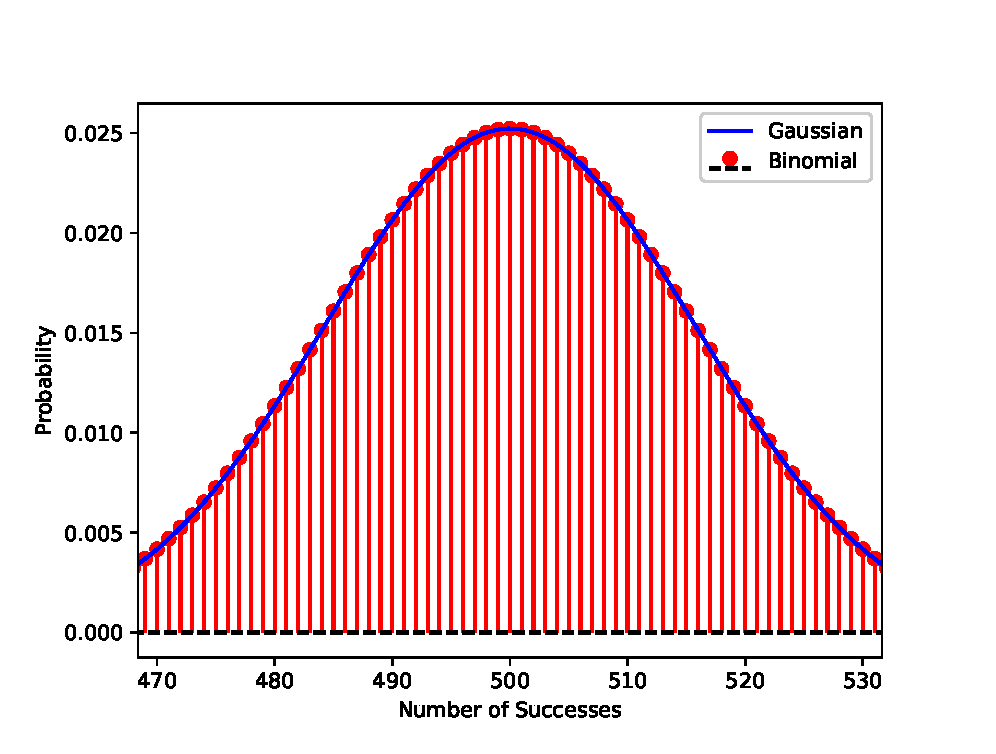
\includegraphics[width=\columnwidth]{ncert/12/13/6/4/figs/1000.eps}
  \caption{1000 trails}
  \label{fig:ncert/12/13/6/4/2}
%\end{subfigure}
\end{figure}
\end{enumerate}

\chapter{Identities}
\begin{enumerate}[label=\thechapter.\arabic*,ref=\thechapter.\theenumi]
\numberwithin{equation}{enumi}
\numberwithin{figure}{enumi}
\numberwithin{table}{enumi}
\item 
Let 
\begin{align}
	N = R+B+G, n = r+b+g
\end{align}
where $R,B,G$ and $r,b,g$ represent the number of red, blue and green marbles respectively within $N$ and $n$.  Then
\begin{align}
	\pr{r,b,g} = 
	\frac{\comb{R}{r}
	\comb{B}{b}
	\comb{G}{g}}
{
	\comb{R+B+G}{r+b+g}
}
\label{eq:ncert/11/16/4/1/1}
\end{align}
\solution 
		The number of ways of choosing $n$ marbles from $N$ is 
\begin{align}
	\comb{N}{n}
\end{align}
The number of ways of choosing r,b,g marbles is
\begin{align}
	\comb{R}{r}
	\comb{B}{b}
	\comb{G}{g}
\end{align}
Using the definition of probability, we obtain
\eqref{eq:ncert/11/16/4/1/1}.
\item 
\begin{align}
	 \comb{R+B}{n} = \sum_{k = 0}^{R} \sum_{m = n-k}^{B} \comb{R}{k} \comb{B}{m}
 \label{eq:ncert/11/16/4/1/5}
\end{align}
\solution Since
\begin{align}
	\brak{x+1}^R &= \sum_{k = 0}^{R} \comb{R}{k} \, x^k,
 \label{eq:ncert/11/16/4/1/4}
\\
	\brak{x+1}^R \brak{x+1}^B &= \sum_{k = 0}^{R} \sum_{m = 0}^{B} \comb{R}{k} \comb{B}{m}\, x^{k+m}\\
\implies	\brak{x+1}^{R+B} &= \sum_{k = 0}^{R} \sum_{m = n-k}^{B} \comb{R}{k} \comb{B}{m}\, x^{n} + \sum_{k = 0}^{R} \sum_{m \ne n-k}^{B} \comb{R}{k} \comb{B}{m}\, x^{k+m}\\
\end{align} 
yielding
 \eqref{eq:ncert/11/16/4/1/5}
upon comparing the coefficients of $x^n$ on both sides.
\end{enumerate}

\chapter{Random Number Genration Using Shift Registers}
\iffalse
\documentclass[12pt]{article}
\usepackage{graphicx}
\usepackage[none]{hyphenat}
\usepackage[english]{babel}
\usepackage{caption}
\usepackage[parfill]{parskip}
\usepackage{hyperref}
\usepackage{import}
\usepackage{booktabs}
\usepackage{circuit}%%Importing Packing circiut.sty created for circuit
\def\inputGnumericTable{}
\usepackage{color}                                            
    \usepackage{array}                                            
    \usepackage{longtable}                                        
    \usepackage{calc}                                             
    \usepackage{multirow}                                         
    \usepackage{hhline}                                           
    \usepackage{ifthen}
\usepackage{array}
\usepackage{amsmath}  
\usepackage{circuitikz}
\usepackage{parallel,enumitem}
\usepackage{listings}
\lstset{
language=tex,
frame=single,
breaklines=true
}
 
\begin{document}
\fi
%\subsection{Random Number Genration using Shift Registers}
\subsection{Components}
%\begin{table}[!h]
%\centering
\input{random_number/figs/components.tex}

\renewcommand{\theequation}{\theenumi}
\renewcommand{\thefigure}{\theenumi}
\begin{enumerate}[label=\thesubsection.\arabic*.,ref=\thesubsection.\theenumi]
\numberwithin{equation}{enumi}
\numberwithin{figure}{enumi}
\numberwithin{table}{enumi}
\item Generate the CLOCK signal using the 555 timer circuit as shown in the figure \ref{fig:1}
\begin{figure}[!ht]
\includegraphics[width=7cm, height=6cm]{random_number/figs/555.png}
\label{fig:1}
\end{figure}	
	
\item Connect the CLOCK output of 555 timer circuit to CLOCK signal of D-Flip flops, change the resistor value to 1M$\Omega$		
\item Now make the cicuit for shift registers uisng 4 D-Flip flops (by using two 7474 IC's) and one X-OR gate (7486 IC) as shown in figure \ref{fig:2}. Pin out for 7474 IC is shown in figure \ref{fig:7447}
\begin{figure}
\centering
\subimport{random_number/figs/}
{circuit1.tex}
\caption{Circuit Connections}
\label{fig:2}
\end{figure}

\begin{figure}[!ht]
\begin{center}

\includegraphics[width=11cm, height=6cm]{random_number/figs/IC7474.png}
\label{fig:7474}

\end{center}
\end{figure}
\item Connect the output of each D-flip flop to Decoder IC (7447 IC), The pin out of 7447 IC is shown in figure \ref{fig:7447}
\begin{figure}[!ht]
\begin{center}
\resizebox {\columnwidth} {!} {
\input{random_number/figs/7447.tex}
}
\end{center}
\caption{}
\label{fig:7447}
\end{figure}
\item As per the pinout of IC 7474 [2,12] pins of both IC's need to connected to the [7,1,2,6] of decoder IC respectively
\item Make connections between the seven segment display in Fig\ref{fig:sevenseg} and the 7447 IC in Fig.\ref{table:7447_disp} as shown in Table 2.1
\begin{table}[!ht]
\centering
\input{random_number/figs/7447_disp.tex}
\caption{}
\label{table:7447_disp}
\end{table}
\begin{figure}[!ht]
\begin{center}
\resizebox {0.3\columnwidth} {!} {
\input{random_number/figs/sevenseg.tex}
}
\end{center}
\caption{}
\label{fig:sevenseg}
\end{figure}
\item Additionally make conections like Vcc and GNG to every IC as per the respective IC pinout for IC's 7474,7447,7486.
\end{enumerate}

\chapter{NCERT}
\begin{enumerate}[label=\thechapter.\arabic*,ref=\thechapter.\theenumi]
\numberwithin{equation}{enumi}
\numberwithin{figure}{enumi}
\numberwithin{table}{enumi}
\item Two Coins are tossed once, where
\begin{enumerate}[label=(\roman*)]
\item  E : Tail appears on one coin,\qquad F : one coin shows head
\item  E : no tail appears,\qquad\qquad\qquad F : no head appears
\end{enumerate}
\end{enumerate}

\latexprintindex

\end{document}

 
